% Options for packages loaded elsewhere
\PassOptionsToPackage{unicode}{hyperref}
\PassOptionsToPackage{hyphens}{url}
%
\documentclass[
  a4paper,12pt,twoside,onecolumn,openright,final,oldfontcommands]{memoir}
\title{Traitement des mots abstraits}
\author{}
\date{\vspace{-2.5em}}

\usepackage{amsmath,amssymb}
\usepackage{lmodern}
\usepackage{iftex}
\ifPDFTeX
  \usepackage[T1]{fontenc}
  \usepackage[utf8]{inputenc}
  \usepackage{textcomp} % provide euro and other symbols
\else % if luatex or xetex
  \usepackage{unicode-math}
  \defaultfontfeatures{Scale=MatchLowercase}
  \defaultfontfeatures[\rmfamily]{Ligatures=TeX,Scale=1}
\fi
% Use upquote if available, for straight quotes in verbatim environments
\IfFileExists{upquote.sty}{\usepackage{upquote}}{}
\IfFileExists{microtype.sty}{% use microtype if available
  \usepackage[]{microtype}
  \UseMicrotypeSet[protrusion]{basicmath} % disable protrusion for tt fonts
}{}
\makeatletter
\@ifundefined{KOMAClassName}{% if non-KOMA class
  \IfFileExists{parskip.sty}{%
    \usepackage{parskip}
  }{% else
    \setlength{\parindent}{0pt}
    \setlength{\parskip}{6pt plus 2pt minus 1pt}}
}{% if KOMA class
  \KOMAoptions{parskip=half}}
\makeatother
\usepackage{xcolor}
\IfFileExists{xurl.sty}{\usepackage{xurl}}{} % add URL line breaks if available
\IfFileExists{bookmark.sty}{\usepackage{bookmark}}{\usepackage{hyperref}}
\hypersetup{
  pdftitle={Traitement des mots abstraits},
  hidelinks,
  pdfcreator={LaTeX via pandoc}}
\urlstyle{same} % disable monospaced font for URLs
\usepackage{longtable,booktabs,array}
\usepackage{calc} % for calculating minipage widths
% Correct order of tables after \paragraph or \subparagraph
\usepackage{etoolbox}
\makeatletter
\patchcmd\longtable{\par}{\if@noskipsec\mbox{}\fi\par}{}{}
\makeatother
% Allow footnotes in longtable head/foot
\IfFileExists{footnotehyper.sty}{\usepackage{footnotehyper}}{\usepackage{footnote}}
\makesavenoteenv{longtable}
\usepackage{graphicx}
\makeatletter
\def\maxwidth{\ifdim\Gin@nat@width>\linewidth\linewidth\else\Gin@nat@width\fi}
\def\maxheight{\ifdim\Gin@nat@height>\textheight\textheight\else\Gin@nat@height\fi}
\makeatother
% Scale images if necessary, so that they will not overflow the page
% margins by default, and it is still possible to overwrite the defaults
% using explicit options in \includegraphics[width, height, ...]{}
\setkeys{Gin}{width=\maxwidth,height=\maxheight,keepaspectratio}
% Set default figure placement to htbp
\makeatletter
\def\fps@figure{htbp}
\makeatother
\setlength{\emergencystretch}{3em} % prevent overfull lines
\providecommand{\tightlist}{%
  \setlength{\itemsep}{0pt}\setlength{\parskip}{0pt}}
\setcounter{secnumdepth}{5}
\newlength{\cslhangindent}
\setlength{\cslhangindent}{1.5em}
\newlength{\csllabelwidth}
\setlength{\csllabelwidth}{3em}
\newlength{\cslentryspacingunit} % times entry-spacing
\setlength{\cslentryspacingunit}{\parskip}
\newenvironment{CSLReferences}[2] % #1 hanging-ident, #2 entry spacing
 {% don't indent paragraphs
  \setlength{\parindent}{0pt}
  % turn on hanging indent if param 1 is 1
  \ifodd #1
  \let\oldpar\par
  \def\par{\hangindent=\cslhangindent\oldpar}
  \fi
  % set entry spacing
  \setlength{\parskip}{#2\cslentryspacingunit}
 }%
 {}
\usepackage{calc}
\newcommand{\CSLBlock}[1]{#1\hfill\break}
\newcommand{\CSLLeftMargin}[1]{\parbox[t]{\csllabelwidth}{#1}}
\newcommand{\CSLRightInline}[1]{\parbox[t]{\linewidth - \csllabelwidth}{#1}\break}
\newcommand{\CSLIndent}[1]{\hspace{\cslhangindent}#1}
%%%%%%%%%%%%%%%%%%%%%%%%%%%%%%%%%%%%%
% Loading (other) relevant packages %
%%%%%%%%%%%%%%%%%%%%%%%%%%%%%%%%%%%%%

%\usepackage[latin1]{inputenc} % special characters with pdflatex
%\usepackage[utf8]{inputenc} % special characters with pdflatex
%\inputencoding{latin1} % special characters with pdflatex

\usepackage{fontspec} % special characters (e.g., accents) with xelatex or lualatex
\usepackage{pdflscape} % figures in landscape mode
\usepackage{tikz} % creating graphic elements
\usepackage{lscape} % figures or tables in landscape mode
%\usepackage{indentfirst} % indents first pragraph after section header
\usepackage{float} % improves the interface for defining floating objects (e.g., figures or tables)
\usepackage[flushleft]{threeparttable} % allows for three part tables with a specified notes section
\usepackage[many]{tcolorbox} % provides environment for colored boxes
\usepackage{pdfpages} % simplifies the inclusion of PDF documents

\usetikzlibrary{intersections} % used to determine lines intersections
\tcbuselibrary{listings,breakable} % ...

\usepackage{pifont} % provides commands for pi fonts (e.g., dingbats, symbol)
\usepackage{graphicx} % provides optionnal arguments to the \includegraphics command
\usepackage{geometry} % provides an easy and flexible user interface to customize page layout
\usepackage{longtable} % allows writing tables that extend on several pages
\usepackage{supertabular} % the predecessor of the longtable package
\usepackage{scrextend} % uses components of KOMA-Script
\usepackage{tabularx} % defines the tabularx environment
\usepackage{lscape} % modifies the margins and rotates the page contents but not the page number.
\usepackage{tabu} % provides flexible latex table environment (e.g., long table)
\usepackage{array} % an extended implementation of the array and tabular environments
\usepackage[gen]{eurosym} % provides the euro (€) symbol
\usepackage{gensymb} % provides the degree (°) symbol
\usepackage{subfig} % provides support for the manipulation and reference of small or ‘sub’ figures and tables within a single figure or table environment
\usepackage{stackrel,amssymb}
\usepackage{textcomp} % provides many text symbols
\usepackage{setspace} % provides support for setting the spacing between lines
\usepackage{microtype} % makes better looking pdf
\usepackage{booktabs,caption,fixltx2e} % ...
\usepackage[none]{hyphenat} % removes hyphenation
% \usepackage[a4paper]{./cover/cover_page} % specifies the path to the cover page template

% https://texblog.org/2012/07/03/fancy-latex-chapter-styles/
% hokusai_28 <- as.character(met.brewer(name = "Hokusai1", n = 28) )
% hokusai_28[c(4, 9, 15, 21, 24, 26, 28)]
% hokusai_28[c(3, 6, 16, 20, 22, 24, 26)]
\definecolor{hokusai1}{HTML}{8D3F31}
\definecolor{hokusai2}{HTML}{BB574A}
\definecolor{hokusai3}{HTML}{E4A45D}
\definecolor{hokusai4}{HTML}{D9C37B}
\definecolor{hokusai5}{HTML}{B1BB89}
\definecolor{hokusai6}{HTML}{87A98D}
\definecolor{hokusai7}{HTML}{547A76}

% varying color per chapter
\newcommand\chaptercolor{gray}

\newcommand{\changechaptercolor}[1]{
  \renewcommand\chaptercolor{#1}
}

%%%%%%%%%%%%%%%%%%%%%%%%%%%%%%%%%%%%%%%%%%%%%%%%%%%%%%%%%%%%%%%%%%%%%
% Below is the by-default configuration of bookdown-demo            %
% https://github.com/rstudio/bookdown-demo/blob/master/preamble.tex %
%%%%%%%%%%%%%%%%%%%%%%%%%%%%%%%%%%%%%%%%%%%%%%%%%%%%%%%%%%%%%%%%%%%%%

%%%%%%%%%%%%%%%%%%%%%%%%
% Remove default title %
% https://stackoverflow.com/questions/45963505/coverpage-and-copyright-notice-before-title-in-r-bookdown
%%%%%%%%%%%%%%%%%%%%%%%%

\let\oldmaketitle\maketitle
\AtBeginDocument{\let\maketitle\relax}

%%%%%%%%%%%%%%%%%%%%%%%%%%%%%%%%%%%%%%%%%%%%%%%%%%%%%%%%%%%%%
% Add a lettrine to the very first character of the content %
%%%%%%%%%%%%%%%%%%%%%%%%%%%%%%%%%%%%%%%%%%%%%%%%%%%%%%%%%%%%%

\usepackage{lettrine} % supports various dropped capitals styles

% https://tex.stackexchange.com/questions/23477/fancy-chapter-headings
% https://texdoc.org/serve/lettrine.pdf/0
% https://tex.stackexchange.com/questions/370579/place-a-box-behind-first-letter-in-chapter-to-stylize
% \lettrine[findent=3pt, nindent=0pt, ante=\rlap{\color{LightSalmon!50}\rule[-0.55\LettrineHeight]{\LettrineWidth}{0.65\LettrineHeight}} ]

\newcommand{\initialgray}[1]{
	\lettrine[lines=3,lhang=0.33,nindent=0em]{
		\color{gray}
		% \color{nattier5}
     		{\textsc{#1}}}{}}

\newcommand{\initial}[1]{
	\lettrine[lines=3,lhang=0.33,nindent=0em]{
		% \color{black}
		\color{gray}
     		{\textsc{#1}}}{}}

%%%%%%%%%%%%%%%%%%%%%%%%%%%%%%%%%%%%%%%%%%%%%%%%%%%%%%%%%%%%%
% Format of the page (block, header, margins, etc.)         %
% https://texdoc.net/texmf-dist/doc/latex/memoir/memman.pdf %
%%%%%%%%%%%%%%%%%%%%%%%%%%%%%%%%%%%%%%%%%%%%%%%%%%%%%%%%%%%%%

% Sets the "real" paper size (already set by a4paper class option)
% \setstocksize{11in}{8.5in}

% Trimmed paper size (trimmed on the left and right)
% \settrimmedsize{11in}{8.5in}{*}

% Sets the \headheight and \footskip parameters (respectively)
\setheadfoot{\onelineskip}{2\onelineskip}

% Sets space between header and block
\setheaderspaces{*}{2\onelineskip}{*}

% Spine and trim page margins from main typeblock (left and right margins if oneside)
\setlrmarginsandblock{25mm}{25mm}{*}

% Top and bottom page margins from main typeblock
\setulmarginsandblock{25mm}{*}{1}

% Applies and enforces the layout
\checkandfixthelayout

% Ensures single spacing between sentences
\frenchspacing

%%%%%%%%%%%%%%%%%%%%%%%%%%%%%%%%%%%%%%%%%%%%%%%%%%%%%%%%%%%%%%%%%%%%%%%%%%%%%%%
%%%%%%%%%%%%%%%%%%%%%%%%%%%%%%%%%%%%%%%%%%%%%%%%%%%%%%%%%%%%%%%%%%%%%%%%%%%%%%%
% Chapter style (taken and slightly modified from Lars Madsen Memoir Chapter) %
%%%%%%%%%%%%%%%%%%%%%%%%%%%%%%%%%%%%%%%%%%%%%%%%%%%%%%%%%%%%%%%%%%%%%%%%%%%%%%%
%%%%%%%%%%%%%%%%%%%%%%%%%%%%%%%%%%%%%%%%%%%%%%%%%%%%%%%%%%%%%%%%%%%%%%%%%%%%%%%

%%%%%%%%%%%%%%%%%%%%%%%%%%%%%%%%%%%%%%%%%%%%%%%%%%%%%%%%%%%%%%%%%%
% Fonts
% -------------------------------------------------------
% Best LaTeX fonts: https://r2src.github.io/top10fonts/
% https://www.quora.com/Which-is-a-good-font-choice-for-writing-a-PhD-thesis-I-have-provisionally-chosen-CharterITC-but-I-am-not-sure-about-it-I-think-the-best-way-to-go-is-a-serif-font-but-I-dont-want-a-classic-look-but-something-more-updated
%https://tex.stackexchange.com/questions/59702/suggest-a-nice-font-family-for-my-basic-latex-template-text-and-math/59706
% https://www.overleaf.com/learn/latex/Font_typefaces
%%%%%%%%%%%%%%%%%%%%%%%%%%%%%%%%%%%%%%%%%%%%%%%%%%%%%%%%%%%%

% \usepackage{libertine} % nice font

% \usepackage{mathpazo} % using the Palatino font (nice font but does not work with the \oe and breaks cover page)
% \usepackage{palatino} % nice font but does not work with the \oe... and no math support
% \usepackage{fouriernc} % font with math support: New Century Schoolbook (nice font but does not work with the \oe...)
% \usepackage{charter} % using the Charter font (nice font but does not work with the \oe...)

% \usepackage{fourier} % using the Utopia font (nice font but does not work with the \oe...)

%%%%%%%%%%%%%%%%%%%%%%%%
% Formatting
%%%%%%%%%%%%%%%%%%%%

\usepackage{calc} % simple arithmetics in latex commands
\usepackage{soul} % hyphenation for letterspacing, underlining, etc.

% new from http://www.ebookation.com/wp-content/uploads/2010/03/memoirchapstyles.pdf
% \newsavebox{\ChpNumBox}
% \newcommand*{\thickhrulefill}{%
%   \leavevmode\leaders\hrule height 1\p@ \hfill \kern \z@}
% \newcommand*\BuildChpNum[2]{%
%   \begin{tabular}[t]{@{}c@{}}
%     \makebox[0pt][c]{#1\strut}  \\[.5ex]
%     \colorbox{ChapBlue}{%
%       \rule[-10em]{0pt}{0pt}%
%       \rule{1ex}{0pt}\color{black}#2\strut
%       \rule{1ex}{0pt}}%
%   \end{tabular}}

\makeatletter
\newlength\dlf@normtxtw
\setlength\dlf@normtxtw{\textwidth}
\newsavebox{\feline@chapter}
\newcommand\feline@chapter@marker[1][4cm]{%
	\sbox\feline@chapter{%
		\resizebox{!}{#1}{\fboxsep=1pt%
			\colorbox{\chaptercolor}{\color{white}\thechapter}%
		}}%
		\rotatebox{90}{%
			\resizebox{%
				\heightof{\usebox{\feline@chapter}}+\depthof{\usebox{\feline@chapter}}}%
			{!}{\scshape\so\@chapapp}}\quad%
		\raisebox{\depthof{\usebox{\feline@chapter}}}{\usebox{\feline@chapter}}%
}

\newcommand\feline@chm[1][4cm]{%
	\sbox\feline@chapter{\feline@chapter@marker[#1]}%
	\makebox[0pt][c]{% aka \rlap
		\makebox[1cm][r]{\usebox\feline@chapter}%
	}}

\makechapterstyle{daleifmodif}{
\renewcommand\chapnamefont{\normalfont\Large\scshape\raggedleft\color{\chaptercolor}}
\renewcommand\chaptitlefont{\normalfont\Large\bfseries\scshape}
\renewcommand\chapternamenum{}
\renewcommand\printchaptername{\color{\chaptercolor}}
\renewcommand\printchapternum{\null\hfill\feline@chm[2.5cm]\par}
\renewcommand\afterchapternum{\par\vskip\midchapskip}
\renewcommand\printchaptertitle[1]{\color{\chaptercolor}\chaptitlefont\raggedleft
  % \renewcommand\chaptername{Chapter}
  % \renewcommand\chaptername{\color{nattier5}{Chapitre}}
  ##1\par}

}

\makeatother
\chapterstyle{daleifmodif}

% The pages should be numbered consecutively at the bottom centre of the page
\makepagestyle{myvf}
\makeoddfoot{myvf}{}{\thepage}{}
\makeevenfoot{myvf}{}{\thepage}{}
\makeheadrule{myvf}{\textwidth}{\normalrulethickness}
\makeevenhead{myvf}{\small\textsc{\leftmark}}{}{}
\makeoddhead{myvf}{}{}{\small\textsc{\rightmark}}
\pagestyle{myvf}

%%%%%%%%%%%%%%%%%%%%%%%%%%%%%%%%%%%%%%%%%%%%%%%%%%%%%%%%%%%%%%%%%%%%%%%%%%%%%%%%%%%%%%%%%%%%%%%%%%%%%%%%
% https://tex.stackexchange.com/questions/126155/how-to-set-colored-ruled-margins-for-some-pages
%%%%%%%%%%%%%%%%%%%%%%%%%%%%%%%%%%%%%%%%%%%%%%%%%%%%%%%%%%%%%%%%%%%%%%%%%%%%%%%%%%%%%%%%%%%%%%%%%%%%

\usetikzlibrary{calc}
\usepackage{fancyhdr}

\fancypagestyle{mypage}{%
    \fancyhf{}
    % \fancyhead[LO]{%
    %     \begin{tikzpicture}[overlay,remember picture]
    %         \fill [color=nattier5] (current page.north west) rectangle
    %             ($ (current page.south west) + (1cm,0cm) $);
    %     \end{tikzpicture}
    %     }
    % \fancyhead[RE]{%
    %     \begin{tikzpicture}[overlay,remember picture]
    %         \fill [color=nattier5](current page.north east) rectangle
    %             ($ (current page.south east) + (-1cm,0cm) $);
    %     \end{tikzpicture}
    %     }
    \fancyfoot[C]{\thepage}
    \renewcommand{\headrulewidth}{0pt}
    \renewcommand{\footrulewidth}{0pt}
}

%%%%%%%%%%%%%%%%%%%%%%%%%%%%%%%%%%%%%%%%%%%%%%%%%%%%%%%%
% Create summary box to put at the end of each chapter %
%%%%%%%%%%%%%%%%%%%%%%%%%%%%%%%%%%%%%%%%%%%%%%%%%%%%%%%%

% https://tex.stackexchange.com/questions/172475/how-can-i-define-a-custom-tcolorbox-environment-with-color-as-a-parameter

\newtcolorbox[]{summary}[3][]{
    fonttitle=\bfseries,
    breakable,
    colframe = #3!90,
    colback = #3!10,
    title=#2,
    #1
    }

%%%%%%%%%%%%%%%%%%%%%%%%%%%%%%%%%%%%%%
% Create explanation Box environment %
%%%%%%%%%%%%%%%%%%%%%%%%%%%%%%%%%%%%%%

\tcbuselibrary{skins,breakable}

\newtcolorbox[auto counter, number within = chapter, number freestyle = {\noexpand\thechapter.\noexpand\arabic{\tcbcounter}}]{mybox}[3][]{%
    breakable,
    colframe = #3!90,
    colback = #3!10,
    fonttitle = \bfseries,
    title = Encart~\thetcbcounter: #2,
    #1
    }

%%%%%%%%%%%%%%%%%%%%%%%%%%%%%%%%%%%%%
% Get the number of current chapter %
%%%%%%%%%%%%%%%%%%%%%%%%%%%%%%%%%%%%%

\newcommand\getcurrentref[1]{
 \ifnumequal{\value{#1}}{0}
  {??}
  {\the\value{#1}}
}

%%%%%%%%%%%%%%%%%%%%%%%%
% Insert an empty page %
%%%%%%%%%%%%%%%%%%%%%%%%

\usepackage{afterpage} % executes command after the next page break

\newcommand\blankpage{%
    \null
    \thispagestyle{empty}%
    % \addtocounter{page}{-1}% % uncomment to increase page counter
    \newpage
    }

\newcommand{\clearemptydoublepage}{\newpage{\thispagestyle{empty}\cleardoublepage}}

%%%%%%%%%%%%%%%%%%
% Epigraph style %
%%%%%%%%%%%%%%%%%%

\usepackage{epigraph} % provides commands to assist in the typesetting of a single epigraph

\setlength\epigraphwidth{1\textwidth}
\setlength\epigraphrule{0pt} % no line between
\setlength\beforeepigraphskip{1\baselineskip} % space before and after epigraph
\setlength\afterepigraphskip{2\baselineskip}
\renewcommand*{\textflush}{flushright}
\renewcommand*{\epigraphsize}{\normalsize\itshape}

%%%%%%%%%%%%%%%%%%%%%
% Break url in LOFs %
%%%%%%%%%%%%%%%%%%%%%

\PassOptionsToPackage{hyphens}{url}
\usepackage{hyperref} % extensive support for hypertext in latex

%%%%%%%%%%%%%%%%%%%%%%%%%%%
% Fixing landscape tables %
%%%%%%%%%%%%%%%%%%%%%%%%%%%

% solution from https://github.com/crsh/papaja/issues/287

% Manuscript styling
\usepackage{csquotes} % provides advanced facilities for inline and display quotations.
\usepackage{upgreek} % provides the upright Greek letters from the Euler or Adobe Symbol fonts
\captionsetup{font=singlespacing,justification=justified}

% Table formatting
% \usepackage{longtable} % allows writing tables that extend on several pages
% \usepackage{lscape} % figures or tables in landscape mode
% \usepackage[counterclockwise]{rotating} % Landscape page setup for large tables
\usepackage{multirow}	% table styling
\usepackage{tabularx}	% control column width
\usepackage[flushleft]{threeparttable} % allows for three part tables with a specified notes section
\usepackage{threeparttablex} % lets threeparttable work with longtable

% Create new environments so endfloat can handle them
% \newenvironment{ltable}
%   {\begin{landscape}\begin{center}\begin{threeparttable}}
%   {\end{threeparttable}\end{center}\end{landscape}}
\newenvironment{lltable}{\begin{landscape}\begin{center}\begin{ThreePartTable}}{\end{ThreePartTable}\end{center}\end{landscape}}

% Enables adjusting longtable caption width to table width
% Solution found at http://golatex.de/longtable-mit-caption-so-breit-wie-die-tabelle-t15767.html
\makeatletter
\newcommand\LastLTentrywidth{1em}
\newlength\longtablewidth
\setlength{\longtablewidth}{1in}
\newcommand{\getlongtablewidth}{\begingroup \ifcsname LT@\roman{LT@tables}\endcsname \global\longtablewidth=0pt \renewcommand{\LT@entry}[2]{\global\advance\longtablewidth by ##2\relax\gdef\LastLTentrywidth{##2}}\@nameuse{LT@\roman{LT@tables}} \fi \endgroup}

%%%%%%%%%%%%%%%%%%%%%%%%%%%
% My (APA6) caption style %
%%%%%%%%%%%%%%%%%%%%%%%%%%%

\usepackage{caption} % provides many ways to customise captions in floating environments
\captionsetup[figure]{labelsep=period,labelfont={it,normalsize},textfont={normalsize}}

%%%%%%%%%%%%%%%%%%%%%%%%%%%%%%%%%%%%%%%%%%%%%%%%%%%%%%%%%%%
% Removing extra vertical blank spaces between paragraphs %
%%%%%%%%%%%%%%%%%%%%%%%%%%%%%%%%%%%%%%%%%%%%%%%%%%%%%%%%%%%

\raggedbottom

%%%%%%%%%%%%%%%%%%%%%%%%%%%%%%%%%%%%%%%%%%%%%%%%%%%%
% Command used in the manual list of abbreviations %
%%%%%%%%%%%%%%%%%%%%%%%%%%%%%%%%%%%%%%%%%%%%%%%%%%%%

\newcommand\nomenclature[2]{#1 & #2 \\}

%%%%%%%%%%%%%%%%%%%%%%%%%%%%%%%%%%%%%%%%%%%%%%%%%%%%%%%%%%%%%%%%%%%%%%%%%%%%%%%%%%%
% Commands used for the AMU title page
% https://github.com/SCD-Aix-Marseille-Universite/latexamu-intro/blob/main/main.tex
%%%%%%%%%%%%%%%%%%%%%%%%%%%%%%%%%%%%%%%%%%%%%%%%%%%%%%%%%%%%%%%%%%%%%%%%%%%%%%%%%%%

% \documentclass[paper=a4,fontsize=12pt,DIV=calc]{scrreprt}
% \usepackage[utf8]{inputenc}
% \usepackage[T1]{fontenc}
% \usepackage{lmodern}
% \usepackage[english,french]{babel}
% \usepackage[english,main=french]{babel}
\usepackage[french]{babel}
% \usepackage[babel]{csquotes}
\usepackage{csquotes}
% \MakeAutoQuote{«}{»}

% \usepackage[a4paper, pass]{geometry}
% \usepackage{graphicx}
% \usepackage{xcolor}
% \usepackage{multicol}
% \usepackage[colorlinks=true, urlcolor=blue]{hyperref}

\DisemulatePackage{setspace}
\usepackage{setspace}

\usepackage{tikz}
\usetikzlibrary{decorations.markings}
\definecolor{blueamu}{RGB}{0, 101, 189}
\definecolor{cyanamu}{RGB}{61, 183, 228}
\newcommand{\dhorline}[3][0]{%
    \tikz[baseline=-2pt]{\path[decoration={markings,
      mark=between positions 0 and 1 step 2*#3
      with {\node[color=blueamu, fill, circle, minimum width=#3, inner sep=0pt, anchor=south west] {};}},postaction={decorate}]  (0,#1) -- ++(#2,0);}}
\newcommand{\dvertline}[3][0]{%
    \tikz[baseline=2em]{\path[decoration={markings,
      mark=between positions 0 and 1 step 2*#2
      with {\node[color=black!50, fill, circle, minimum width=#2, inner sep=0pt, anchor=south west] {};}},postaction={decorate}] (0, #1) -- ++(0,#3);}}

% \graphicspath{{fig/}{logo/}}

\newcommand\titel[1]{{\usefont{T1}{tit}{el}{n} #1 }}
\newcommand\titl[1]{{\usefont{T1}{tit}{l}{n} #1 }}
\newcommand\titm[1]{{\usefont{T1}{tit}{m}{n} #1 }}
\newcommand\titsb[1]{{\usefont{T1}{tit}{sb}{n} #1 }}
\newcommand\titb[1]{{\usefont{T1}{tit}{b}{n} #1 }}

% \makeatletter\newcommand\HUGE{\@setfontsize\Huge{28}{0}}\makeatother
% \renewcommand\listfigurename{Liste des figures}
% \renewcommand\listtablename{Liste des tableaux}

%%%%%%%%%%%%%%%%%%%%%%%%%%%%%%%%%%%%%%%%%%%%%%%%%%%%%%%%%%%%%%%%%%%%%%%%
% removes par indent and par skip
%%%%%%%%%%%%%%%%%%%%%%%%%%%%%%%%%%%%%%%%%%%%%%%%%%%%%%%%%%%%%%%%

% \usepackage{parskip} % http://ctan.org/pkg/parskip
% \setlength{\parindent}{0pt}

% https://tex.stackexchange.com/questions/22553/memoir-parskip-package
\setlength{\parindent}{0pt}
\nonzeroparskip
\ifLuaTeX
  \usepackage{selnolig}  % disable illegal ligatures
\fi

\begin{document}
\maketitle

\setmainfont{Titillium}
\newgeometry{margin=2em}
%\newgeometry{margin=20mm}
\thispagestyle{empty}

\begin{center}
	\begin{minipage}[c]{.5\linewidth}
		\raggedright
\includegraphics[height=6em]{logos/logo_amu_excellence}
	\end{minipage}\hfill
	\begin{minipage}[c]{.5\linewidth}
		\raggedleft
\includegraphics[height=6em]{logos/logo_lpc.png}
	\end{minipage}\hfill
\end{center}

\vspace{1em}

\begin{center}
	\begin{minipage}[c]{.6\linewidth}
		\dhorline{\textwidth}{4pt}
	\end{minipage}\hfill
	\begin{minipage}[c]{.4\linewidth}
		\raggedleft{NNT/NL : 2022AIXM0147/009ED356}
		% renseigner votre numéro national de thèse (NNT) et le numéro local (NL)
		% ils sont indiqués sur la page d'informations administratives de votre espace de dépôt dans le guichet de dépôt légal des thèses AMU lorsque votre date de soutenance est renseignée par votre service de scolarité
		% https://depot-theses.univ-amu.fr/
	\end{minipage}\hfill
\end{center}

%\vspace{1em}
%\doublespacing
\begin{flushleft}
    \huge\textbf{\textcolor{cyanamu}{THÈSE DE DOCTORAT}}\\
	\Large Soutenue à Aix-Marseille Université\\
	% \titl{\Large dans le cadre d'une cotutelle avec}\\
	\Large le 5 mai 2022 par\\
\end{flushleft}

\vspace{1em}

\begin{center}
	\Huge \textbf{Camille GRASSO}\\
    \vspace{1em}
	\LARGE Traitement des mots abstraits : comment le corps et le mouvement ancrent le concept de temps dans notre architecture cognitive
\\
\end{center}

\singlespacing

\vspace{2em}
%\vspace{4em}

\begin{center}
	\begin{minipage}[t]{.35\linewidth}
    	    \vspace{.5em}
        	\textbf{Discipline}

        	%\titl{Cognition, Langage, Éducation}
        	Cognition, Langage, Éducation

    	    \vspace{1em}
        	\textbf{Spécialité}

        	Psychologie

    	    \vspace{1em}
        	\textbf{École doctorale}

        	École Doctorale 356

    	    \vspace{1em}
        	\textbf{Laboratoire de recherche}

        	Laboratoire de Psychologie Cognitive

	\end{minipage}\hfill
	\begin{minipage}[t]{.03\linewidth}
	    \dvertline{4pt}{-20em}
	\end{minipage}\hfill
	\begin{minipage}[t]{.6\linewidth}
	    \vspace{0.5em}
    	\textbf{Composition du jury}

	    \vspace{1em}
    	%\titel{
      \noindent\begin{tabular}{@{}p{16em} p{14em}}
        \textbf{Pr. Sylvie DROIT-VOLET} & Rapportrice\\
      	Université Clermont Auvergne & Présidente du jury\\
        \\
      	\textbf{Dr. Ludovic FERRAND} & Rapporteur\\
      	CNRS, Université Clermont Auvergne\\
        \\
      	\textbf{Dr. Véronique BOULENGER} & Examinatrice\\
      	CNRS, Université Lyon 2\\
      	\\
        \textbf{Dr. Kristof STRIJKERS} & Examinateur\\
      	CNRS, Aix-Marseille Université\\
        \\
      	\textbf{Dr. Johannes ZIEGLER} & Directeur de thèse\\
      	CNRS, Aix-Marseille Université\\
      	\\
      	\textbf{Dr. Marie MONTANT} & Co-Directrice de thèse\\
      	Aix-Marseille Université\\
      \end{tabular}
        %}
	\end{minipage}\hfill
\end{center}

% \vspace{1em}

% \begin{center} % logos partenaires
% 	\begin{minipage}[c]{.25\linewidth}
% 		% \centering\includegraphics[height=5em]{example-image-a}
% 		\centering
\includegraphics[height=6em]{logos/logo_lpc.png}
% 	\end{minipage}\hfill
% 	\begin{minipage}[c]{.25\linewidth}
% 		\centering\includegraphics[height=5em]{example-image-b}
% 	\end{minipage}\hfill
% 	\begin{minipage}[c]{.25\linewidth}
% 		\centering\includegraphics[height=5em]{example-image-c}
% 	\end{minipage}\hfill
% 	\begin{minipage}[c]{.25\linewidth}
% 		\centering\includegraphics[height=5em]{example-image-c}
% 	\end{minipage}\hfill
% \end{center}

\restoregeometry

%%%%%%%%%%%%%%%%%%%%%%%%%%%%%%
% End of title page template %
%%%%%%%%%%%%%%%%%%%%%%%%%%%%%%

% starting page numbering (roman style)
\pagenumbering{roman}

% leaving an empty page between cover page and rest of the content
\blankpage

% using the font
% \setmainfont{Linguistics Pro}
\setmainfont{Heuristica}

% increasing line spacing to 1.5 (but leaving footnote to 1)
% \OnehalfSpacing
\setstretch{1.5}

\chapter*{Affidavit}

Je soussignée, Camille Grasso, déclare par la présente que le travail présenté dans ce manuscrit est mon propre travail, réalisé sous la direction scientifique de Johannes Ziegler et Marie Montant, dans le respect des principes d'honnêteté, d'intégrité et de responsabilité inhérents à la mission de recherche. Les travaux de recherche et la rédaction de ce manuscrit ont été réalisés dans le respect à la fois de la charte nationale de déontologie des métiers de la recherche et de la charte d'Aix-Marseille Université relative à la lutte contre le plagiat. Ce travail n'a pas été précédemment soumis en France ou à l'étranger dans une version identique ou similaire à un organisme examinateur.

\vspace{\baselineskip}

Fait à Marseille, le 25 février 2022.

\afterpage{\blankpage}

\chapter*{Liste des publications et participation aux conférences}

\textbf{Liste des publications}

\begin{enumerate}
\def\labelenumi{\arabic{enumi}.}
\item
  \textbf{Grasso, C. L.}, Ziegler, J. C., Mirault, J., Coull, J. T., \& Montant, M. (2021). As time goes by: Space-time compatibility effects in word recognition. \emph{Journal of Experimental Psychology: Learning, Memory, and Cognition}. \url{https://doi.org/10.1037/xlm0001007}
\item
  \textbf{Grasso, C. L.}, \& Montant, M. (2018). Body-blindness in language studies. \emph{L'Année psychologique, 118}(4), 383-388. \url{http://doi.org/10.3917/anpsy1.184.0383}
\end{enumerate}

\textbf{Articles soumis à publication}

\begin{enumerate}
\def\labelenumi{\arabic{enumi}.}
\item
  \textbf{Grasso, C. L.}, Ziegler, J. C., Coull, J., \& Montant, M. (2021, November 25). Eye movements through space interfere with visual processing of time-related words. \url{https://doi.org/10.31234/osf.io/mhaxd}
\item
  \textbf{Grasso, C. L.}, Ziegler, J. C., Coull, J., \& Montant, M. (2022, February 1). Embodied time: Effect of reading expertise on the spatial representation of past and future. \url{https://doi.org/10.31234/osf.io/qkz9r}
\end{enumerate}

\textbf{Participation aux conférences et écoles d'été au cours de la période de thèse}

\emph{Communications orales invitées}

\begin{enumerate}
\def\labelenumi{\arabic{enumi}.}
\tightlist
\item
  Grasso, C. L. (2019). \emph{L'effet de congruence spatio-temporelle en langage}. Conférence à la Journées Rencontres Jeunes Chercheur-ses. Laboratoire de Psychologie et de NeuroCognition (LPNC), Grenoble, France.
\end{enumerate}

\newpage

\emph{Communications orales}

\begin{enumerate}
\def\labelenumi{\arabic{enumi}.}
\tightlist
\item
  Grasso, C. L. (2019). \emph{La langue incarnée: un voyage dans l'espace-temps}. Séminaire Embodiment: Le rôle du corps dans la cognition. Faculté des Lettres, Aix-Marseille, France.
\end{enumerate}

\emph{Communications affichées}

\begin{enumerate}
\def\labelenumi{\arabic{enumi}.}
\item
  Grasso, C. L. (2019). \emph{As time goes by: space-time compatibility effects in word recognition}. European Society of Cognitive Psychology (ESCoP). Tenerife, Espagne.
\item
  Grasso, C. L. (2019). \emph{As time goes by: space-time compatibility effects in word recognition}. Embodied and situated language processing (ESLP). Umbolt-Universität, Berlin, Allemagne.
\item
  Grasso, C. L. (2018). \emph{Why older adults improve performance after experiencing success: the role of strategic variations}. Journée d'étude du vieillissement (JEV). Chambéry, France.
\end{enumerate}

\afterpage{\blankpage}

\chapter*{Résumé}

\initial{L}'individu se nourrit d'un ensemble de concepts dont il n'a pourtant aucune expérience sensorielle et motrice. Cette capacité à transcender le monde physique pour construire un univers de représentations abstraites, comme celle de temps, est considérée comme l'une des plus sophistiquées de la cognition humaine. Si l'implication des processus sensorimoteurs dans le traitement des mots concrets est aujourd'hui établie, leur rôle dans le traitement des mots abstraits est au cœur d'un vif débat. À partir de propositions théoriques comme celles de la réutilisation neuronale et de l'apprentissage par corrélation, nous proposons une piste explicative de l'ancrage des concepts abstraits temporels. Dans une série de cinq études, nous avons mis en évidence le rôle du mouvement dans l'émergence d'effets de congruence spatio-temporelle lors du traitement de mots liés au temps. Plusieurs propositions théoriques peuvent êtes faites à la lumière de nos résultats. La première est que le concept de temps pourrait s'ancrer directement dans l'expérience temporelle qui accompagne le mouvement. En ce sens, les chevauchements entre temps et espace n'impliqueraient pas que le temps soit intrinsèquement de nature spatiale, mais que temps et espace soient confondus parce que vécus ensemble via le mouvement. La deuxième est que les mécanismes qui sous-tendent la représentation et le traitement des concepts temporels pourraient réutiliser ceux de la planification motrice et de la cognition spatiale. La troisième est que l'action répétée de lecture et d'écriture pourrait constituer l'expérience sensorimotrice de premier ordre qui définit le cadre d'ancrage de temps, et lie ensemble espace et temps.

\vspace{\baselineskip}

\textbf{Mots-clés} : Cognition incarnée, Reconnaissance visuelle de mots, Mouvement, Concepts abstraits, Temps, Espace

\afterpage{\blankpage}

\chapter*{Abstract}

\initial{H}umans are equipped with a set of concepts of which they have no perceptive or motor experience. This capacity to transcend the physical world to build a universe of abstract representations, such as astrophysics or time, is one of the most sophisticated of human cognition. If the involvement of sensorimotor processes in the processing of concrete words is now established, their role in the representation and the processing of abstract concepts is at the heart of a lively debate. Based on a detailed review of data from the literature, and theoretical proposals such as neural reuse and correlational learning, we examined the way in which temporal abstract concepts could be grounded. In a series of five experiments, we investigated the role of movement in the emergence of space-time congruency effects during the visual processing of words conveying temporal information. Overall, our results suggest that movement plays a key role for the grounding (and the processing) of the temporal content of these words. Considering our results, several theoretical propositions (not exclusive) can be made. First, the abstract concept of time could be directly grounded in the temporal experience that accompanies the execution of the movement. In this sense, the overlaps between time and space would not imply that time is intrinsically spatial in nature, but that time and space are generally confused because they are experienced together through movement. Second, the mechanisms underlying the representation and processing of temporal concepts could reuse those of motor planning and spatial cognition. Third, the repeated action of reading and writing could constitute the sensorimotor experience that links space and time together.

\vspace{\baselineskip}

\textbf{Key-words}: Embodied cognition, Visual word processing, Movement, Abstract concepts, Time, Space

\afterpage{\blankpage}

\chapter*{Remerciements}

\initial{E}n toute transparence, si cette partie trône fièrement dans les premières pages de ce manuscrit, elle est en réalité rédigée bien après le point final du dernier chapitre. En fait, l'ampleur de ma gratitude me semble difficilement exprimable avec des mots. Cependant, je vais essayer -- bien que maladroitement - de rendre hommage aux incroyables personnes qui composent mon existence, qui m'ont accepté dans leur espace personnel, qui ont contribué à la qualité de ce travail, mais aussi (et surtout) qui m'ont communiqué l'envie et la joie de faire ce beau métier.

Il m'a semblé cohérent d'organiser ces remerciements à l'image de cette thèse. Comme ce travail traite de la représentation conceptuelle désignée par un mot, je tenterai d'attribuer aux personnes remerciées un ensemble de mots qui, selon moi, les désignent.

Mes premiers remerciements et ma profonde gratitude se dirigent vers mes encadrant·e·s, sans qui je ne serais certainement pas en train d'écrire ces quelques lignes, et avec qui j'espère pouvoir continuer à échanger et collaborer encore de nombreuses années. À vous trois, et chacun à votre manière, vous représentez les caractéristiques de la chercheuse que j'aspire à être.

Je remercie chaleureusement ma directrice \textbf{Marie Montant}, un modèle d'intelligence, de détermination, d'empathie, et de modestie, que chacun devrait suivre. Marie, merci de m'avoir accordé ta confiance, de m'avoir motivée, canalisée, et guidée tout au long de ce parcours. Ton esprit et ton énergie ont contribué de façon significative à l'évolution de ma pensée, et ainsi à faire de moi la chercheuse que je suis aujourd'hui. Je suis particulièrement reconnaissante de t'avoir eu comme mentor et tellement heureuse de cette belle relation que nous avons développée au-delà du cadre traditionnel.

Mes pensées se dirigent ensuite naturellement vers mon directeur \textbf{Johannes Ziegler}, un chercheur passionné, aux capacités de réflexions surprenantes, et un puits de connaissance hors du commun. Johannes, je te remercie sincèrement pour ta confiance, pour le temps précieux que tu m'as accordé en dépit de tes nombreuses responsabilités et de la charge titanesque de travail que tu abats au quotidien. Le tout sans jamais faiblir, en restant disponible et en faisant tout pour les nombreuses personnes qui t'entourent (on se demande même si tu dors la nuit\ldots). Je m'estime extrêmement chanceuse de t'avoir comme mentor. Merci pour tout ce que tu es et tout ce que tu m'as transmis, parfois même sans t'en rendre compte.

Enfin, je souhaite adresser de chaleureux remerciements à ma directrice de l'ombre, \textbf{Jennifer Coull}, une chercheuse extraordinaire, inspirante, brillante, et modeste, au sourire contagieux et réconfortant. Jenny, je ne te remercierai jamais assez pour tout ce que tu as fait (sans condition ni contrepartie) pour me permettre d'être là où je suis aujourd'hui, mais aussi pour tout ce que tu m'as transmis. Tu es l'une des principales raisons qui font que j'aime ce métier et tu représentes, selon moi, la preuve que l'on peut être à la fois une excellente chercheuse, une femme épanouie, une mère, et une amie.

Mes remerciements se dirigent à présent vers mon jury de thèse : \textbf{Pr. Sylvie Droit-Volet}, \textbf{Dr.~Ludovic Ferrand}, \textbf{Dr.~Véronique Boulenger}, et \textbf{Dr.~Kristof Strijkers}, qui ont accordé un temps précieux pour lire et examiner cette thèse. Je vous remercie également pour votre présence le jour de cette soutenance. Je vous remercie notamment pour ces discussions passionnantes et stimulantes que nous avons eues. À l'avenir, j'espère avoir la chance d'échanger de nouveau avec vous, et, pourquoi pas, collaborer sur des sujets qui nous animent.

Mes affectueux remerciements à \textbf{Christine Assaiante}, qui m'a accueillie, accompagnée, et soutenue tout au long de mon parcours. Christine, je te remercie d'avoir cru en moi et de m'avoir donné la force de continuer dans un moment où je doutais de moi. Je te remercie également pour toutes nos discussions et les précieux apprentissages que tu m'as apportés.

Je remercie également les deux piliers du Laboratoire de Psychologie Cognitive, \textbf{Frédéric Lombardo} et \textbf{Colette Pourpe}, pour leur gentillesse, leur travail titanesque, et nos nombreux échanges.

J'adresse mes remerciements à \textbf{Marie-Hélène}, pour sa gentillesse, nos discussions matinales et pour avoir allumé le chauffage d'appoint dans notre bureau tôt le matin avant notre arrivée pour nous éviter de souffrir du froid.

Mes pensées se dirigent également à mes enseignant·e·s de master au LPNC à Grenoble. Je tiens à remercier tout particulièrement \textbf{Christopher Moulin} et \textbf{Céline Souchay}, deux chercheur·euses brillant·e·s, les premiers à avoir cru en moi (bien avant moi), qui m'ont transmis leur passion pour la recherche et ont tout fait pour me permettre de suivre cette voie.

Je souhaite vivement remercier mes amis. Un immense merci à mon très cher et vieil ami, \textbf{Thomas Ferrari}, mon Jiminy Cricket à moi, à l'esprit, l'humour (caustique !), la curiosité, et l'humilité incroyables. Peu de mots sont disponibles pour exprimer à quel point je m'estime chanceuse de vivre cette belle (et inconditionnelle) amitié qui fête sa première décennie. Thomas, je te remercie pour m'avoir accompagnée et épaulée toutes ces années. Merci pour ces innombrables et stimulantes discussions de plusieurs heures qui nous paraissent toujours ne durer que quelques minutes. Merci d'être mon ami, simplement, en dépit du temps et de l'espace qui nous séparent. Parce que ta présence dans ma vie, même de loin, participe à faire de moi la personne que je suis et à rendre ma vie si douce.

Un grand merci à mon cher ami \textbf{Jonathan Mirault}, chercheur impliqué et rigoureux, incroyable technicien, et au cœur sur la main. Jon, ma \emph{`dino-patate douce'}, les mots me manquent pour exprimer toute ma reconnaissance, non seulement pour ton amitié mais aussi pour tout ce que tu m'as appris. Sans toi et le temps que tu m'as accordé, je n'en serais pas là aujourd'hui, merci. Merci, pour cette amitié pure et simple qui nous lie, et ces riches moments ensemble, que j'espère encore nombreux.

Un grand merci à ma très chère amie \textbf{Fleur Brun}, jeune fofolle attachante, à l'esprit complexe et farfelu, au cœur tendre, qui a tout de suite pris une place importante dans ma vie. Fleur, \emph{`Tu fais bien ce que tu veux'}, je suis tellement heureuse de t'avoir dans ma vie, merci pour tous ces moments de bonheur brut, ces bonnes bouff', ces heures de jeux (quand je gagne), ces fous rires incontrôlables, et d'avoir partagé mon quotidien pendant deux ans. Merci de m'avoir accompagnée, supportée, suivie dans mes folies vertes, culinaires, et musicales. Je suis fière de pouvoir te compter parmi mes amis et espère que cela va durer encore de belles et nombreuses années.

Je ne saurais comment remercier convenablement mon très cher ami \textbf{Jean-Patrice Albrand}, au sourire contagieux, à l'insatiable curiosité, et à la générosité débordante. Jypé, \emph{`ça va les mollets ?'}, merci pour tous ces instants de bonheur brut, de danses jusqu'au bout de la nuit, de rires, pour les balades nature, les vacances, les bonnes bouff', ces discussions, ces soirées jeux, et j'en passe. Merci d'avoir toujours été présent, dans les moments de joie mais aussi les moments de doutes, merci de m'avoir accompagnée, écoutée, et reboostée. Mon ami, \emph{mon frérot}, tu participes de façon significative à rendre ma vie intéressante et douce. Et s'il te plaît : ne change jamais !

Merci à \textbf{Guillem Bonnafos}, cette machine à la force surhumaine et au mental d'acier, intelligent, drôle, simple, et modeste. Guillem, \emph{`c'est transcendantal et cosmique, la vérité vraie'}, je te remercie pour ton énergie, de toujours répondre présent, que ce soit pour boire un verre ou pour aider. Aujourd'hui, je suis heureuse de pouvoir te compter parmi mes amis (je l'espère encore très longtemps) et mes humains préférés. \textbf{Rebecca Marchetti}, une jeune chercheuse prometteuse, au cœur sur la main et à la force inépuisable. Rebecca, je suis impressionnée et admirative de ton parcours. Merci d'être mon amie et de rendre ma vie si belle. \textbf{Manon Rouselle}, ma danseuse déterminée, intelligente, drôle, et douce. Manon, merci pour ton amitié, ta générosité sans limite et ton sourire contagieux. Merci pour ces moments, j'ai hâte de vivre les prochains. Merci à \textbf{Julie Lassault}, \emph{`merci, mais non merci'}, la meuf incroyable (et qui ne s'en rend même pas compte) qui a fait une thèse, retapé une maison, et est devenue mère, le tout en même temps !! Julie, merci de m'avoir remarquée au labo et de m'avoir mise à l'aise. Merci pour ces barres de rire à m'en faire mal au ventre et pour cette amitié qui ne faiblit pas, malgré nos emplois du temps capricieux. Merci à \textbf{Simonetta Logreco}, mon rayon de soleil Italien, à la créativité débordante et inarrêtable. Simonetta, \emph{`Simo'}, quelle rencontre ! Merci de faire partie de ma vie, de m'avoir soutenue, de m'avoir nourrie de tes mets délicieux et de ta culture étonnante. Merci à \textbf{Yannick Becker}, artiste et photographe de talent la nuit, génial, généreux et brillant. Yannick, merci pour ton amitié, ton soutien infaillible, pour nos discussions stimulantes et ces cours incroyables que nous avons donnés ensemble. Merci à \textbf{Eva Vives}, pour tous ces bons moments passés ensemble, tout particulièrement cette soirée « vin et éthique scientifique » inoubliable. Merci également à \textbf{Edouard Alavoine}, cet esprit attachant, drôle et farfelu, pour son amitié et les bons moments passés ensemble, \emph{`arrrrrrrête'}. Merci à \textbf{Ludivine Javouret}, \emph{`tu vois ce que je veux dire ?'}, pour m'avoir accueillie chez toi, et aidée, à plusieurs reprises, pour les passations dans les écoles.

Merci à \textbf{Maëlle Tixier}, jeune chercheuse dynamique, rigoureuse, et à l'esprit vif. Merci pour cette belle amitié et ton soutien pendant toutes ces années. Nos nombreuses correspondances par mail tout au long de cette thèse ont contribué de façon non négligeable à me donner la force et l'envie de persévérer dans les moments difficiles.

Je remercie vivement mes chers voisin·e·s du 13 qui sont devenus de vrais amis. Par ordre d'arrivée, je remercie d'abord ma chère voisine \textbf{Nicole Negrel}, cette femme à l'histoire de vie incroyable qui devrait être publiée, dont la générosité dépasse l'entendement. Nicole, je te remercie pour avoir été une voisine si gentille, et pour tous ces rires que nous avons eus dans le couloir, j'espère que nous en vivrons de nombreux autres. Merci à \textbf{Sixtine}, cette grande et belle femme drôle, déterminée, au cœur sur la main, et aux mille et unes activités (on se demande aussi comment elle trouve le temps de faire tout ça). Sixtine, merci d'avoir toqué à ma porte et d'avoir insisté pour me sortir de ma grotte, merci pour le lombrithé, et merci de rester mon amie en dépit de notre départ. Merci également à \textbf{Quentin}, ce génie fou aux deux doctorats (oui, deux !), génial, drôle et généreux, pour nos premiers échanges sur le palier qui stimulent la matière grise, les soirées jeux / bouff', et pour ce déguisement incroyable.

Je remercie aussi chaleureusement \textbf{Sophie Tinard}, \emph{`framboise'}, cette femme drôle, généreuse et inspirante qui a été ma première amie sur Mars'. Merci Sophie, pour ta gentillesse et ta simplicité, pour m'avoir accueillie et `adoptée,' pour m'avoir laissé entrer dans ton monde, fait découvrir tant de choses et pour tous ces précieux moments ensemble. Merci à \textbf{Morgane}, incroyable femme avant d'être une incroyable Maman, la reine du dancefloor. Merci à \textbf{Maria}, cette femme géniale, créative et déterminée, pour son amitié et son soutien. J'en profite pour remercier toute l'équipe, affiliée de prés ou de loin à `La graine' : \textbf{Mael}, la pile électrique qui a toujours la patate et le sourire, la formidable et sublime \textbf{Farah} infatigable et adorable, \textbf{Édouard}, l'ami fidèle et cuisinier hors pair, \textbf{Thomas}, discret au cœur tendre, \textbf{Clémence}, l'alliance parfaite entre douceur et folie, aux punchlines fatales, \textbf{Anthonin} l'aventurier joyeux et attachant, \textbf{Max}, au sourire contagieux et aux playlists pointues, \emph{`il fait lourd non?'}. Je vous suis tellement reconnaissante pour m'avoir accueillie à bras ouverts et pour avoir rendu ma vie Marsienne si belle toutes ces années. Merci pour ces purs moments, que la distance et le temps ne peuvent effacer.

Je remercie chaleureusement les membres du laboratoire. Merci à \textbf{Françoise Vitu-Thibault}, qui a accepté sans hésitation d'apporter son aide et son expertise en Eyetracking. Merci à \textbf{Marlène Abadie}, à la fois chercheuse brillante, enseignante dévouée, et une collègue drôle et généreuse. Merci à \textbf{F.-Xavier Alario}, ce chercheur rigoureux, à l'esprit vif et aux remarques toujours constructives et intelligentes. Merci à \textbf{Pascale Colé}, rigoureuse et passionnée, pour toutes ces discussions stimulantes que nous avons eues. Merci à \textbf{Isabelle Dautriche}, chercheuse passionnée impliquée dans la vie du laboratoire et, pour sa gentillesse et nos échanges toujours riches. Merci à \textbf{Jérémy Danna}, chercheur incroyable (e.g., a écrit son HDR à la main), généreux et qui accepte sans hésiter d'aider toute personne qui en aurait besoin (e.g., moi). Enfin, un immense merci à \textbf{Jean-Luc Anton}, pour nos échanges toujours stimulants, pour sa gentillesse hors du commun, et pour m'avoir donné confiance en moi à plusieurs reprises (certainement sans le savoir).

Enfin, j'adresse des remerciements tout particuliers à \textbf{Carole Parron}. Si ces remerciements ne pourront malheureusement jamais lui parvenir, je tiens à exprimer ici mes sincères pensées à cette femme extraordinaire. Je la remercie pour avoir été la première chercheuse à m'accueillir au laboratoire avec son large sourire, à avoir été la première à s'être intéressée à moi, la jeune étudiante timide. Aussi, merci Carole pour m'avoir écoutée et motivée à poursuivre, et merci pour nos échanges par mails réconfortants et motivants.

Un immense merci à l'ensemble de mes collègues doctorant·e·s, post-doctorant·e·s, et chercheur·euses, qui m'ont accompagnée dans cette belle aventure, présentés sans ordre particulier ici : \textbf{Karen Davranche, Éric Castet, Ambre Denis-Noël, Leonardo Pinto Arata, Loic Bonnier, Thibault Gajdos, Isabelle Regner, Marjorie Armando, Marco Bressan, Gabriel Weindel, Boris Burle, Maud Rasamimanana, Laure Tosatto, Stéphane Dufau, Agnes Blaye, Christelle Guette, Jean-Baptiste Melmi, Camille Lallement, Jonathan Grainger, Iliana Kotwas, Anaïs Cauna, Felipe Pegado, Aurélie Calabrese, Elisa Gavard, Angélique Roquet, Konstantina Margiotoudi, Yufei Tan, Thomas Chartier, Joël Fagot, Florence Gaunet, Angélique Lamontagne, Adrien Meguerditchian, Arnaud Rey}.

Enfin, je remercie chaleureusement l'ensemble des participant·e·s de nos études. Je remercie également chaleureusement les enseignant·e·s de l'école La Vernette pour avoir accepté, à deux reprises, de nous accueillir dans leur classe. Je remercie également tous les enfants qui ont participé avec joie et curiosité à ces deux sessions d'expérimentations. Tout ceci n'aurait jamais été possible sans leur participation.

J'ai également eu la chance incroyable d'enseigner pendant ces années de thèse. Rien n'est plus stimulant et gratifiant que de pouvoir transmettre et échanger sur des sujets passionnants. J'adresse donc mes remerciements chaleureux à l'ensemble des étudiant·e·s à qui j'ai eu l'honneur d'enseigner. Je les remercie pour leur motivation, leurs gentils mots qui m'ont légitimée et donné confiance dans mon enseignement.

Pour terminer (ne dit-on pas \emph{`le meilleur pour la fin'} ?) il m'importe de remercier ma famille. Tout d'abord, merci à mes parents, dont la générosité, la bienveillance et l'humilité n'ont pas d'égal. Merci non seulement pour votre amour inconditionnel, mais aussi (et surtout) pour m'avoir offert le choix et l'opportunité que vous n'avez jamais eus. Cette thèse n'est rien à côté du travail et des sacrifices que vous avez fournis pour me permettre de faire ce métier. Je suis donc chanceuse, heureuse et fière d'être votre fille.

Merci à \textbf{mon père}, une force de la nature inépuisable et hors du commun, dont l'intelligence, la sagesse, la patience et la persévérance m'inspirent et me guident depuis toujours.
Papa, \emph{`La cuillère n'existe pas'}. Trouver les mots qui apaisent les maux de son enfant ne doit pas être chose aisée. C'est pourtant avec cette phrase, d'apparence simple, que tu as su me réconforter dans les moments de doute et me donner le courage de persévérer. Sans oublier ton humour, toujours là pour faire rire, en dépit des circonstances.
Merci à \textbf{ma mère}, cette femme qui accomplit des choses extraordinaires sans s'en apercevoir. Sa générosité et son dévouement pour les personnes qui l'entourent n'ont pas de limite. Et, même si elle en doute parfois, ce sont ces traits, couplés à sa curiosité, sa créativité, et sa sensibilité que j'admire et qui me façonnent. Maman, \emph{`Ma bichette'}.

Je remercie mes sœurs, \textbf{Céline et Mélissa}, de grandes et belles femmes avant d'être de supers mamans, sans qui ma vie aurait été bien vide. Merci pour leur soutien sans faille, leur amour et tous les précieux moments passés ensemble. Je remercie aussi chaleureusement mes deux supers beaux-frères, \textbf{Nicolas et Anthony}, qui, chacun à leur façon, m'apportent beaucoup de support et de précieuses leçons de vie. Je suis aussi la fière \emph{`tatie d'amour'} de trois enfants extraordinaires qui m'offrent de purs instants de bonheur et d'amour. \textbf{Capucine}, douce et créative, \emph{`Papillon'} (ton premier mot). \textbf{Pénélope}, drôle et brillante, \emph{`Je te vois'}. \textbf{Tino}, pile sur pattes au cœur sur la main, \emph{`on va faire un tour de vélo ?'}.

Mes chaleureuses pensées vont également à \textbf{Claire}, \textbf{Antoine}, \textbf{Ida} et \textbf{François}, ma super belle-famille, pour leur gentillesse, leur accueil, et tous les bons moments que nous avons déjà passés ensemble.

Enfin, mes plus affectueuses pensées et remerciements vont à \textbf{Ladislas Nalborczyk}, \emph{`mais nooooon'}, sans aucun doute la personne la plus incroyable qui compose mon existence. Il m'est difficile de ne choisir que quelques mots pour le désigner. Cependant, je dirais : brillant, génial, humble, généreux, empathique. Ladislas, le temps passé avec toi est ce que je possède de plus précieux. Ces moments sont les parfaits cas d'étude de distorsions temporelles, là où le temps objectif mesuré par des outils conventionnels ne correspond en rien au temps subjectif ressenti. Ladislas, mon double, merci \ldots{} pour tout! Merci pour ces journées et ces nuits entières à ne rien faire d'autre que parler, pour tous ces rires, ces apprentissages qui nous animent tous les deux et tous ces beaux projets. Merci pour ton soutien pendant ces derniers mois de thèse, pour tes mots réconfortants qui m'ont motivée et ont su me donner confiance en moi. Pour finir, merci de me faire vivre cette chose inestimable qu'on appelle l'amour et à laquelle je ne croyais pas avant de te rencontrer.

\afterpage{\blankpage}

\chapter*{Préface}

\sloppy 

\epigraph{"N'essaie pas de tordre la cuillère, c'est impossible. Tu dois essayer de te concentrer pour faire éclater la vérité : la cuillère n’existe pas."}{The Matrix, Wachowski \& Wachowski, (1999), 1:04:26}

\initial{C}ette citation n'est pas anodine. Elle interroge le sens de notre expérience consciente de l'environnement. Nous pouvons la reformuler ainsi : Si l'objet \emph{cuillère} existe indépendamment de nous dans le monde physique, l'ensemble des connaissances qui définissent pour nous l'objet \emph{cuillère} est le produit fini de multiples processus cognitifs qui nous sont propres. Sa forme visuelle émerge de traitements neuronaux complexes et rapides effectués à partir des photons renvoyés par la surface de la cuillère et captés par nos récepteurs rétiniens. Son percept tactile émerge de la pression qu'exerce ladite cuillère sur les mécanorécepteurs de notre peau. De surcroît, les percepts sensoriels associés à l'objet \emph{cuillère} ne sont pas perçus de façon distincte : ils sont intégrés en un tout cohérent et unique, faisant référence à un même concept, celui de cuillère. Ainsi, en lisant ces lignes, vous pouvez vous représenter toutes les caractéristiques perceptives et sémantiques associées au mot « cuillère », et cela même en l'absence de l'objet \emph{cuillère}. En ce sens, notre représentation conceptuelle du mot ou de l'objet \emph{cuillère} est idiosyncratique : elle est propre à chacun, elle n'existe pas, en dehors de notre esprit.

Théoriquement, savoir que le mot « cuillère » fait référence à l'objet \emph{cuillère}, et accéder à toutes les connaissances associées à ce mot, serait rendu possible par l'activation des mêmes réseaux neuronaux qui sous-tendent nos interactions antérieures avec l'objet \emph{cuillère}. Cette capacité élaborée se développerait via des mécanismes d'apprentissage neuronaux sophistiqués, contraints par notre histoire évolutive -- innés -- et par l'ensemble de nos expériences -- vécues -- au contact de l'objet manipulable désigné par le mot « cuillère ». Intuitivement, de telles propositions théoriques semblent raisonnables lorsqu'il s'agit de concepts concrets, dont l'existence physique est tangible, comme celui de « cuillère ». Cependant, la question de savoir comment le cerveau peut acquérir, raisonner, et comprendre des concepts avec lesquels nous ne pouvons interagir directement via nos sens et nos actions, comme le concept de \emph{temps}, pose un réel défi pour les sciences du langage et de la cognition.

La question que nous posons et développons dans ce manuscrit porte spécifiquement sur ce point : comment un concept abstrait, comme celui de \emph{temps}, peut-il prendre racine dans un ensemble d'expériences sensorimotrices si, par définition, il n'existe pas ? À cet égard, nous proposerons que le mouvement joue un rôle prépondérant dans le traitement des concepts abstraits temporels.\footnote{Les scripts qui ont permis de générer cette thèse sont disponibles via ce lien : \url{https://osf.io/ndqf4/}.}

\clearemptydoublepage

\renewcommand{\contentsname}{Table des matières}
\maxtocdepth{subsection}

\tableofcontents*
\addtocontents{toc}{\par\nobreak \mbox{}\hfill{\bf Page}\par\nobreak}
\newpage

\renewcommand\listfigurename{Liste des figures}

\listoffigures
\addtocontents{lof}{\par\nobreak\textbf{{\scshape Figure} \hfill Page}\par\nobreak}
\newpage

\addcontentsline{toc}{chapter}{Liste des acronymes}
\chapter*{Liste des acronymes}

\begin{longtable}{@{}p{2cm}@{}p{\dimexpr\textwidth-2cm\relax}@{}}

\nomenclature{\textbf{TEP}}{Topographie par Émission de Positons}
\nomenclature{\textbf{IRMf}}{Imagerie par Résonnance Magnétique fonctionnelle}
\nomenclature{\textbf{EEG}}{Électroencéphalographie}
\nomenclature{\textbf{MEG}}{Magnétoencéphalographie}
\nomenclature{\textbf{ACE}}{Action Compatibility Effect}
\nomenclature{\textbf{LASS}}{Language and Situated Simulation}
\nomenclature{\textbf{SNARC}}{Spatial-Numerical Association of Responses Codes}
\nomenclature{\textbf{APC}}{Action-Perception Circuits}
\nomenclature{\textbf{MTL}}{Mental Timeline}
\nomenclature{\textbf{NSU}}{Négligence Spatiale Unilatérale}
\nomenclature{\textbf{ATOM}}{A Theory of Magnitude}
\nomenclature{\textbf{CMT}}{Conceptual Metaphor Theory}
\nomenclature{\textbf{RT}}{Reaction Time}
\nomenclature{\textbf{ER}}{Error Rate}
\nomenclature{\textbf{LME}}{Linear Mixed-Effects}
\nomenclature{\textbf{AIC}}{Akaike Information Criterion}
\nomenclature{\textbf{BIC}}{Bayesian Information Criterion}
\nomenclature{\textbf{DVA}}{Degrees of Visual Angle}
\nomenclature{\textbf{STEARC}}{Spatio-Temporal Association of Response Code}
\nomenclature{\textbf{VWFA}}{Visual Word Form Area}
\end{longtable}

\newpage
\blankpage

\pagenumbering{arabic}

\hypertarget{part-chapitres-thuxe9oriques}{%
\part{Chapitres théoriques}\label{part-chapitres-thuxe9oriques}}

\sloppy
\changechaptercolor{hokusai1}

\hypertarget{chap1}{%
\chapter{Du cognitivisme classique aux théories incarnées du langage}\label{chap1}}

\epigraph{"If, then, one persists in being curious about the 'inner aspect' of behavior and in believing that a man's thoughts are as legitimate objects for scientific study as his movements; if on the other hand, one realizes that it is through his movements that man takes his place in the rest of the order of nature, then the proper outcome of this twofold interest is an attempt to show that the whole of the inner life is correlated with and dependent upon bodily movement."}{Washburn, M. F. (1916, p.xiii)}

\initial{C}ommençons par un exemple. Au rythme des mouvements balistiques linéaires - allant de la gauche vers la droite - que vos yeux réalisent en parcourant ces lignes, vous êtes en train de réaliser une activité d'apparence simple mais dépendante de nombreux processus complexes : la lecture. Chaque mot -- cet ensemble de taches noires qui se détachent du fond blanc -- projeté sur votre rétine se verra associé à un concept, à une représentation porteuse de sens. Par « représentation porteuse de sens », nous faisons référence ici au résultat du processus (ou de l'ensemble de processus) par le(s)quel(s) un mot se verra assigné à une signification, à un concept.

Comme \protect\hyperlink{ref-borghi_words_2014}{Borghi \& Binkofski} (\protect\hyperlink{ref-borghi_words_2014}{2014}), nous associerons le terme « concept » à la signification des mots. Nous l'avons évoqué dans la section précédente ; cette habileté sophistiquée que nous possédons -- celle de donner du sens - serait permise par l'activation des structures cérébrales qui sont engagées lorsque nous interagissons avec l'objet auquel réfère le concept (e.g., \protect\hyperlink{ref-barsalou_grounded_2008}{Barsalou, 2008a}, \protect\hyperlink{ref-barsalou_perceptual_1999}{1999}). À titre d'exemple, la lecture du mot « cuillère » devrait activer les structures corticales motrices en charge des mouvements de notre main, mais aussi des structures corticales visuelles ; et pour ceux qui ont l'habitude de mettre du sucre dans leur café (nécessitant une cuillère pour remuer), il est possible que des structures corticales olfactives et gustatives soient également activées (e.g., \protect\hyperlink{ref-barros-loscertales_reading_2012}{Barrós-Loscertales et al., 2012}; \protect\hyperlink{ref-gonzalez_reading_2006}{González et al., 2006}). Certains auteurs ont utilisé le terme de \emph{simulation} pour désigner cette activation d'aires sensorimotrices et émotionnelles pour accéder au sens d'un mot, à un concept (e.g., \protect\hyperlink{ref-barsalou_cognitive_2008}{Barsalou, 2008b}, \protect\hyperlink{ref-barsalou_perceptual_1999}{1999}; \protect\hyperlink{ref-jeannerod_neural_2001}{Jeannerod, 2001}). Nous adopterons une posture proche, basée sur des notions comme celle de \emph{réutilisation} \emph{neuronale} (e.g., \protect\hyperlink{ref-anderson_neural_2010}{Anderson, 2010}, \protect\hyperlink{ref-anderson_evolution_2007}{2007}; \protect\hyperlink{ref-gallese_neural_2018}{Gallese \& Cuccio, 2018}; \protect\hyperlink{ref-gallese_brains_2005}{Gallese \& Lakoff, 2005}; \protect\hyperlink{ref-sporns_motifs_2004}{Sporns \& Kötter, 2004}) et d'apprentissage par corrélation hebbien (\protect\hyperlink{ref-hebb_organization_1949}{Hebb, 1949}), qui définissent les contours du modèle des circuits d'action-perception (e.g., \protect\hyperlink{ref-pulvermuller_neural_2018}{Pulvermüller, 2018a}, \protect\hyperlink{ref-pulvermuller_neurobiological_2018}{2018b}; \protect\hyperlink{ref-pulvermuller_active_2010}{Pulvermüller \& Fadiga, 2010}), présenté plus en détail dans le chapitre \ref{chap2}.

Indépendamment du niveau d'analyse adopté, les travaux que nous avons menés ne peuvent s'affranchir du cadre théorique dans lequel ils s'inscrivent. Les considérations théoriques adoptées conditionnent notre regard sur le sujet étudié et contraignent les paradigmes expérimentaux qui en découlent. Comme ce travail prend part à un débat théorique sur la nature du langage humain et des mécanismes qui le rendent possible, nous présenterons et discuterons dans ce premier chapitre l'origine des interrogations épistémologiques auquel il tente modestement d'apporter des éléments de réponse.

Précisément, ce premier chapitre contribue à replacer nos travaux dans le débat théorique sur la nature des mécanismes par lesquels l'individu acquière et utilise des représentations conceptuelles abstraites. L'objectif ne sera pas de fournir une revue exhaustive des modèles et des théories du traitement conceptuel, mais de situer la question de l'incarnation des concepts abstraits dans ses racines théoriques. Les questions que nous aborderons dans ce premier chapitre porteront sur i) la nature des processus linguistiques (i.e., modulaires et spécialisés ou distribués et réutilisés) et ii) le contenu des représentations conceptuelles (i.e., modales ou amodales). Nous commencerons par présenter les fondements théoriques du cognitivisme classique, développés et reformulés ensuite dans des théories modulaires et amodales de la cognition et du langage. Il s'agira de montrer comment ces considérations théoriques se sont enracinées dans les sciences cognitives, culminant dans une approche désincarnée de la cognition, où les structures cérébrales périphériques (i.e., servant à l'action, la perception, ou les émotions), n'auraient aucun rôle à jouer dans la cognition.

Nous aborderons ensuite deux limites à cette perspective et que les théories incarnées tentent de résoudre. Premièrement, nous soutiendrons que le principe de modularité -- plus ou moins massive - pour les fonctions cognitives est peu plausible biologiquement. Nous présenterons l'alternative proposée par le principe de réutilisation neuronale tel que développé dans l'hypothèse de redéploiement massif (e.g., \protect\hyperlink{ref-anderson_neural_2010}{Anderson, 2010}, \protect\hyperlink{ref-anderson_after_2014}{2014}). Nous soutiendrons alors que des structures dites de bas niveau (e.g., perceptives, motrices, ou émotionnelles) seraient bien plus profondément impliquées dans les fonctions cognitives dites de haut niveau, comme le langage. C'est dans le sens de la réutilisation neuronale que nous considèrerons le langage comme incarné. Nous proposerons que le langage serait soutenu par la réutilisation de réseaux de neurones préexistants, rendant alors problématique les principes de modules spécialisés à une fonction et, par voie de conséquence, de représentations conceptuelles amodales. Deuxièmement, après avoir présenté les premiers arguments empiriques allant dans ce sens, nous aborderons les discussions encore non résolues que ces observations suscitent. Par exemple, les tenants des modèles modulaires et amodaux du langage considèrent que les propositions théoriques incarnées sont limitées méthodologiquement car elles échouent à rendre compte de concepts auxquels il n'existe aucun accès sensorimoteur : les concepts abstraits (e.g., \protect\hyperlink{ref-goldinger_poverty_2016}{Goldinger et al., 2016}; \protect\hyperlink{ref-mahon_critical_2008}{Mahon \& Caramazza, 2008}). Cette limite interviendra et sera discutée en fin de ce premier chapitre, en guise de transition avec le second.

\hypertarget{naissance-et-essor-du-cognitivisme-classique}{%
\section{Naissance et essor du cognitivisme classique}\label{naissance-et-essor-du-cognitivisme-classique}}

C'est à la cybernétique et au développement des machines de Turing, à l'origine de nos ordinateurs, que l'on doit la naissance du cognitivisme au milieu des années 1950. Sous l'impulsion des travaux de figures telle que Chomsky, Newell, Simon, Fodor, ou encore Pylyshyn, le point de départ qui a conduit à ce que \protect\hyperlink{ref-gardner_minds_1985}{Gardner} (\protect\hyperlink{ref-gardner_minds_1985}{1985}) qualifiera ensuite de « révolution cognitive », a été l'utilisation de la métaphore de l'ordinateur comme modèle théorique pour l'étude de la cognition humaine. Un ordinateur -- en anglais \emph{computer} -- est, comme l'a défini \protect\hyperlink{ref-turing_computing_1950}{Turing} (\protect\hyperlink{ref-turing_computing_1950}{1950}), une machine constituée de logiciels qui exécutent des calculs (des « computations ») sur des symboles. Dans cette optique, à l'image d'un ordinateur, les processus cognitifs sont assimilés à des modules de traitement fonctionnellement distincts et autonomes (\protect\hyperlink{ref-fodor_modularity_1983}{Fodor, 1983}).

Appliqué à la cognition humaine, le postulat alors adopté suppose que toute information externe au système (le signal) serait extraite par des récepteurs pour être ensuite convertie par des mécanismes de transduction dans un format interne désincarné : le symbole (\protect\hyperlink{ref-pylyshyn_computation_1984}{Pylyshyn, 1984}). La transduction se décompose en un mécanisme d'encodage, qui transforme le signal en symbole amodal, et un mécanisme de décodage, qui extrait le sens stocké dans le symbole. \protect\hyperlink{ref-fodor_modularity_1983}{Fodor} (\protect\hyperlink{ref-fodor_modularity_1983}{1983}), suivi de \protect\hyperlink{ref-pylyshyn_computation_1984}{Pylyshyn} (\protect\hyperlink{ref-pylyshyn_computation_1984}{1984}), définissent les symboles comme des représentations amodales du monde externe dotées de valeurs sémantiques traduites et traduisibles par les computations. En effet, pour qu'un symbole puisse être stocké et interprété par le système, il doit être représenté dans un format indépendant de ce qu'il symbolise et de la modalité spécifique du codage dont il a fait l'objet (\protect\hyperlink{ref-newell_computer_1976}{Newell \& Simon, 1976}). Ce n'est qu'après cette étape de construction perceptive que la cognition intervient. Dans ce cadre, la cognition est post-perceptive (i.e., intervenant après l'encodage), ou du moins aperceptive (\protect\hyperlink{ref-anderson_after_2014}{Anderson, 2014}).

En psycholinguistique, cette perspective computo-symbolique et modulaire de la cognition s'est cristallisée dans une approche dite de traitement de l'information. Elle sera notamment illustrée par l'Hypothèse du Système des Symboles Physiques de \protect\hyperlink{ref-newell_computer_1976}{Newell \& Simon} (\protect\hyperlink{ref-newell_computer_1976}{1976}) ou encore les grammaires génératives de \protect\hyperlink{ref-chomsky_syntactic_1968}{Chomsky} (\protect\hyperlink{ref-chomsky_syntactic_1968}{1968}). Pour ces auteurs, penser reviendrait à manipuler des symboles amodaux, c'est-à-dire détachés de toute phénoménologie (voir Figure \ref{fig:chap1-fig1}). Quant aux mécanismes par lesquels l'individu accède au sens des mots (i.e., au concept), nous pouvons citer la proposition faite par les modèles en réseaux formulée par \protect\hyperlink{ref-collins_retrieval_1969}{Collins \& Quillian} (\protect\hyperlink{ref-collins_retrieval_1969}{1969}). Dans ce modèle de traitement de l'information, le sens d'un symbole est extrait des liens que ce dernier entretient avec d'autres symboles. Autrement dit, la valeur sémantique d'un concept serait représentée par des symboles amodaux, eux-mêmes définis par leur relation avec d'autres symboles amodaux (voir encart \ref{symbol}).

\begin{figure}[htbp!]

{\centering 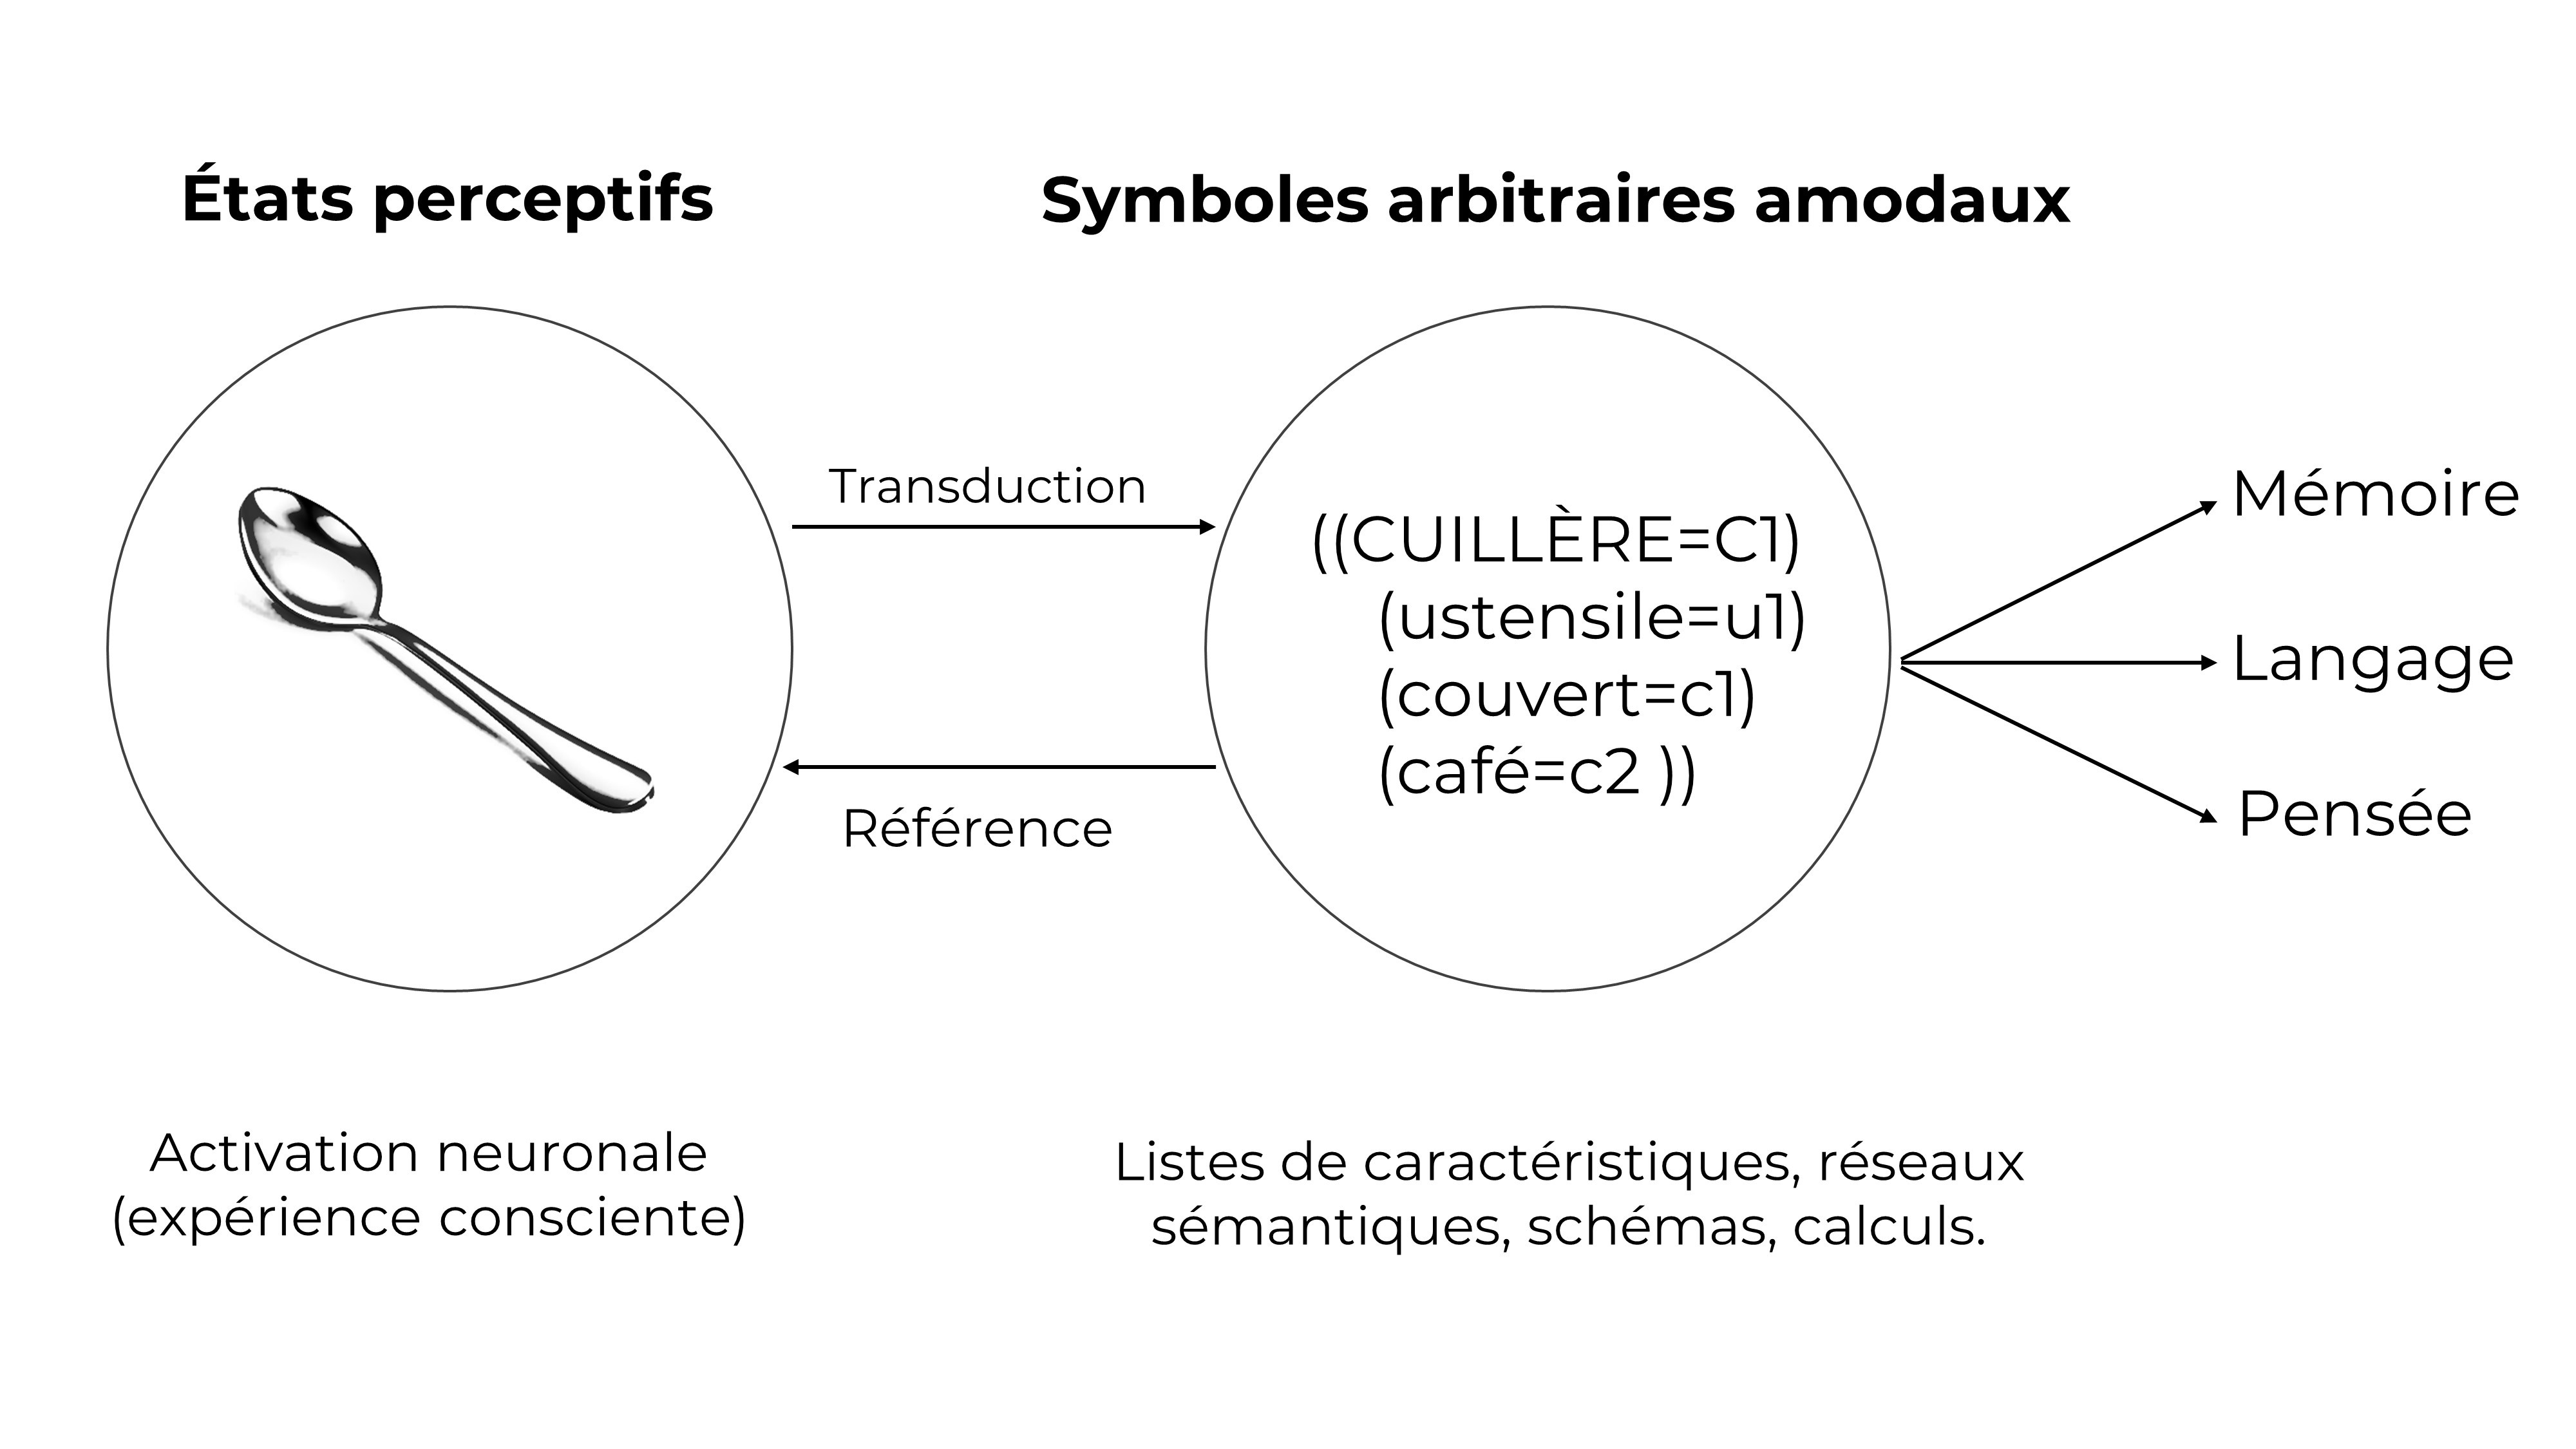
\includegraphics[width=1\linewidth]{figures/chap1-fig1} 

}

\caption{Proposition théorique classique des systèmes de symboles amodaux. Les états perceptifs seraient 'transduits' dans un nouveau format de représentation désincarné : les informations contenues dans ces symboles sont détachées des états perceptifs qui les sous-tendent. Figure adaptée de Barsalou (1999). Notons que le terme 'transduction' est utilisé ici dans son sens Fodorien comme définit plus haut (Fodor, 1983).}\label{fig:chap1-fig1}
\end{figure}

Cependant, la façon dont les symboles conceptuels sont représentés dans le cerveau reste vivement débattue (e.g., \protect\hyperlink{ref-anderson_neural_2016}{Anderson, 2016}, \protect\hyperlink{ref-anderson_neural_2010}{2010}; \protect\hyperlink{ref-barsalou_grounded_2008}{Barsalou, 2008a}, \protect\hyperlink{ref-barsalou_abstraction_2003}{2003}, \protect\hyperlink{ref-barsalou_perceptual_1999}{1999}; \protect\hyperlink{ref-harnad_symbol_1990}{Harnad, 1990}; \protect\hyperlink{ref-pulvermuller_words_1999}{Pulvermüller, 1999}; \protect\hyperlink{ref-searle_minds_1980}{Searle, 1980}; \protect\hyperlink{ref-searle_mystere_1999}{Searle et al., 1999}). Ces considérations théoriques auraient rendu nécessaire le postulat de connaissances préexistantes (i.e., innées), notamment syntaxiques, pour rendre compte de la façon dont le sens est extrait par la manipulation des symboles (e.g., les grammaires génératives de \protect\hyperlink{ref-chomsky_syntactic_1968}{Chomsky, 1968}). Enfin, moins directement, considérer que les systèmes dédiés à la perception et à l'action sont indépendants de la cognition implique la notion de modules de traitement (\protect\hyperlink{ref-anderson_after_2014}{Anderson, 2014}). Ceci est par exemple illustré par (\protect\hyperlink{ref-carruthers_cognitive_2002}{Carruthers, 2002, p. 663}), qui développe le principe de modules de traitement de Fodor et qu'il a baptisé « la conception cognitive du langage » :

\begin{quote}
``What has happened in the cognitive sciences in recent decades, then, is this. Many researchers have become increasingly convinced, by neuropsychological and other evidence, that the mind is more or less modular in structure, built up out of isolable, and largely isolated, components (Barkow et al.~1992; Fodor 1983; Gallistel 1990; Hirschfeld \& Gelman 1994; Pinker 1997; Sachs 1985; Shallice 1988; Sperber et al.~1995). They have also become convinced that the structure and contents of the mind are substantially innate (Carey 1985; Fodor 1981; 1983; Spelke 1994), and that language is one such isolable and largely innate module (Chomsky 1988; Fodor 1983; Pinker 1994).''
\end{quote}

Ainsi, \protect\hyperlink{ref-carruthers_cognitive_2002}{Carruthers} (\protect\hyperlink{ref-carruthers_cognitive_2002}{2002}) résume sa perspective cognitiviste du langage, dans laquelle il fait état de modules isolés de traitement de l'information, qu'il suppose innés et fonctionnant en parfaite autonomie. Dans la section suivante, nous développerons les arguments qui ont conduit à la proposition de modules cognitifs et discuterons des principales limites de cette conception. Nous verrons d'abord brièvement comment les modèles connexionnistes ont répondu à deux limites techniques (i.e., la séquentialité des processus et l'indépendance des modules de traitement). Puis, nous discuterons plus en détail de la notion de modules cognitifs et de la modalité dans laquelle les représentations conceptuelles linguistiques seraient stockées dans le cerveau. Face à ces limites, nous examinerons les propositions alternatives formulées par les théories incarnées de la cognition.

\hypertarget{limites-du-cognitivisme-classique}{%
\section{Limites du cognitivisme classique}\label{limites-du-cognitivisme-classique}}

Si la métaphore du cerveau ordinateur a permis de réintroduire l'étude de la cognition humaine - en tant que système de traitement de l'information - sous une nouvelle matrice interdisciplinaire fructueuse, elle s'est rapidement retrouvée confrontée à plusieurs limites (voir par exemple \protect\hyperlink{ref-barsalou_grounded_2008}{Barsalou, 2008a}, \protect\hyperlink{ref-barsalou_perceptual_1999}{1999}; \protect\hyperlink{ref-glenberg_grounding_2002}{Glenberg \& Kaschak, 2002}; \protect\hyperlink{ref-pulvermuller_words_1999}{Pulvermüller, 1999}; \protect\hyperlink{ref-searle_minds_1980}{Searle, 1980}; \protect\hyperlink{ref-varela_inscription_1983}{Varela et al., 1983}, pour discussions approfondies). Dans leur historique des sciences cognitives, \protect\hyperlink{ref-varela_inscription_1983}{Varela et al.} (\protect\hyperlink{ref-varela_inscription_1983}{1983}) résument que le principal reproche fait au cognitivisme classique est de s'être trop éloigné de la réalité biologique du sujet étudié. Le développement des connaissances sur la physiologie cérébrale a permis l'essor de nombreuses évolutions théoriques que nous pouvons regrouper en deux catégories : les théories modulaires et amodales (e.g., \protect\hyperlink{ref-machery_amodal_2016}{Machery, 2016}; \protect\hyperlink{ref-mahon_critical_2008}{Mahon \& Caramazza, 2008}) et les théories incarnées (e.g., \protect\hyperlink{ref-barsalou_grounded_2008}{Barsalou, 2008a}, \protect\hyperlink{ref-barsalou_perceptual_1999}{1999}; \protect\hyperlink{ref-pulvermuller_neural_2018}{Pulvermüller, 2018a}, \protect\hyperlink{ref-pulvermuller_words_1999}{1999}, \protect\hyperlink{ref-pulvermuller_how_2013}{2013}).

Avant d'introduire les limites des théories modulaires et amodales que les théories incarnées proposent de résoudre, il est important de noter qu'actuellement peu de chercheur·euses considèrent encore pertinente la comparaison entre la cognition humaine et une machine désincarnée qui fonctionnerait sur la base de modules autonomes purement séquentiels. Les modèles connexionnistes ont répondu à de nombreuses limites imputées au cognitivisme classique (cf.~encart \ref{connexionnisme}). Inspirés par les propriétés biophysiques du fonctionnement neuronal, les modèles connexionnistes ont proposé un traitement de l'information non plus \emph{séquentiel} mais \emph{parallèle} et \emph{distribué}, où les modules de traitement ne sont plus \emph{indépendants} et \emph{autonomes} mais \emph{interconnectés}, fonctionnant sur un principe d'\emph{interactions} (e.g., \protect\hyperlink{ref-rumelhart_parallel_1988}{Rumelhart \& McClelland, 1988}; \protect\hyperlink{ref-seidenberg_distributed_1989}{Seidenberg \& McClelland, 1989}).

Bien que ces modèles soient capables de rendre compte de nombreux résultats empiriques -- comme les effets d'amorçage sémantique\footnote{Un effet d'amorçage sémantique se caractérise par des temps de réponse plus rapides pour un item cible lorsqu'il est précédé de la présentation d'un item sémantiquement relié par rapport à un item non sémantiquement relié.} (e.g., \protect\hyperlink{ref-neely_semantic_1991}{Neely, 1991}) -- certains auteur·e·s considèrent que l'explication fournie pour rendre compte de la façon dont la représentation sémantique se construit n'est toujours pas satisfaisante (cf.~encart \ref{symbol}). Les théoricien·ne·s de l'approche incarnée (e.g., \protect\hyperlink{ref-borghi_future_2020}{Borghi, 2020}; \protect\hyperlink{ref-henningsen-schomers_modelling_2021}{Henningsen-Schomers \& Pulvermüller, 2021}; \protect\hyperlink{ref-pulvermuller_concept_1996}{Pulvermüller \& Mohr, 1996}) leur reprochent que le langage demeure localisé dans des modules spécialisées (e.g., \protect\hyperlink{ref-caramazza_cognitive_2006}{Caramazza \& Coltheart, 2006}; \protect\hyperlink{ref-carruthers_cognitive_2002}{Carruthers, 2002}, \protect\hyperlink{ref-carruthers_architecture_2006}{2006}) et les représentations sémantiques continuent d'être amodales. Les sections suivantes nous permettrons de développer et discuter ces deux points.

\newpage

\vspace{2mm}

\begin{mybox}[label = connexionnisme]{L'apport du connexionnisme}{\chaptercolor}

Les théories connexionnistes se sont développées en réponse à deux critiques formulées contre le cognitivisme classique, à savoir le postulat de séquentialité des processus (e.g., Fodor, 1983) et celui d’indépendance des modules responsables du traitement de l’information (e.g., Fodor, 1983; Carruthers, 2002; 2006).\\

Concernant la  \textit{séquentialité} des processus, le développement des connaissances sur le fonctionnement cérébral a rendu peu crédible le principe de traitement séquentiel de l’information. Ce constat est d’ailleurs partagé par McClelland, Hinton, \& Rumelheart (1988), qui résument ainsi le problème : les modèles qui se sont attachés à rendre compte de processus simples – comme la reconnaissance des mots – nécessitent un nombre bien trop élevé d’étapes si elles sont mises en \oe uvre séquentiellement, ce qui est incompatible avec la vitesse d’exécution des processus en question. Ils s’appuient notamment sur les travaux de Feldman \& Ballard (1982) démontrant que les processus seraient bien trop lents pour qu’un tel traitement séquentiel soit plausible. Dès lors, dans la lignée des travaux de Feldman \& Ballard (1982), que Rumelhart, Hinton \& McClelland (1988) proposent un modèle parallèle et distribué du traitement de l'information.\\

Concernant la notion de modules \textit{indépendants} et \textit{autonomes}, le principe de traitement parallèle et distribué est également au cœur du célèbre modèle à Activation Interactive formulé par McClelland \& Rumelheart (1981; 1982), et sera réutilisée ensuite par d’autres modèles connexionnistes de reconnaissance des mots (e.g., Grainger et Jacobs, 1996 ; Grainger \& Holcomb, 2006). Dans cette perspective, les modules de traitement ne sont plus strictement localisés et indépendants mais interconnectés par des connexions bidirectionnelles excitatrices ou inhibitrices soumis à une hiérarchie d’activations parallèles (Grainger \& Holcomb, 2006). 

\end{mybox}

\hypertarget{vers-une-conception-incarnuxe9e-du-langage}{%
\subsection{Vers une conception incarnée du langage}\label{vers-une-conception-incarnuxe9e-du-langage}}

\epigraph{"[...] imagination, like perceiving and doing, is embodied, that is, structured by our constant encounter and interaction with the world via our bodies and brains [...] a key aspect of human cognition is neural exploitation – the adaptation of sensory-motor brain mechanisms to serve new roles in reason and language, while retaining their original functions as well"}{Gallese, V. \& Lakoff, G. (2005, p.456)}

Cette citation de \protect\hyperlink{ref-gallese_brains_2005}{Gallese \& Lakoff} (\protect\hyperlink{ref-gallese_brains_2005}{2005}) résume un principe clé et commun aux théories incarnées du langage, et de la cognition en général. Un principe moteur de ces théories a été de re-situer l'étude du langage dans son cadre biologique et évolutif (e.g., \protect\hyperlink{ref-anderson_neural_2010}{Anderson, 2010}, \protect\hyperlink{ref-anderson_after_2014}{2014}; \protect\hyperlink{ref-gallese_brains_2005}{Gallese \& Lakoff, 2005}; \protect\hyperlink{ref-gibson_ecological_1979}{Gibson, 1979}; \protect\hyperlink{ref-glenberg_what_2007}{Glenberg et al., 2007}). S'il est fait mention d'incarnation, c'est parce que ce cadre théorique repose sur le postulat d'une relation étroite - si ce n'est indivisible - entre la perception, l'action, et la cognition. Dans cette perspective, les structures cérébrales et les structures corporelles qui supportent l'action ou la perception, traditionnellement associées aux fonctions de bas niveau, seraient fonctionnellement et nécessairement impliquées dans les fonctions dites de haut niveau, comme le langage (e.g., \protect\hyperlink{ref-anderson_neural_2010}{Anderson, 2010}, \protect\hyperlink{ref-anderson_after_2014}{2014}; \protect\hyperlink{ref-borghi_language_2012}{Borghi, 2012}; \protect\hyperlink{ref-glenberg_grounding_2002}{Glenberg \& Kaschak, 2002}).

Comme évoqué dans l'introduction de ce chapitre les propositions théoriques d'une cognition incarnée s'ancrent dans un débat théorique non résolu. Si le paradigme incarné est si controversé, c'est probablement parce que les considérations théoriques adoptées sont incompatibles avec deux principes fondateurs des théories cognitives standards (\protect\hyperlink{ref-anderson_neural_2010}{Anderson, 2010}). En effet, bien que les théories incarnées du langage défendent l'idée désormais non controversée que le sens d'un mot est acquis au fil de l'expérience, la question de la nature modulaire et spécialisée du langage ainsi que la nature des représentations sémantiques et conceptuelles (modales ou amodales) dans le cerveau demeurent largement débattues (e.g., \protect\hyperlink{ref-barsalou_grounded_2008}{Barsalou, 2008a}, \protect\hyperlink{ref-barsalou_perceptual_1999}{1999}; \protect\hyperlink{ref-pecher_situating_2005}{Barsalou \& Wiemer-Hastings, 2005}; \protect\hyperlink{ref-pulvermuller_neural_2018}{Pulvermüller, 2018a}).

Dans cette section, nous présenterons d'abord le principe général de modularité corticale et cognitive, représenté majoritairement dans les théories modulaires et amodales (e.g., \protect\hyperlink{ref-dove_beyond_2009}{Dove, 2009}, \protect\hyperlink{ref-dove_need_2011}{2011}; \protect\hyperlink{ref-mahon_critical_2008}{Mahon \& Caramazza, 2008}). Nous examinerons ensuite une proposition alternative au principe de modularité : celui de réutilisation neuronale (e.g., \protect\hyperlink{ref-anderson_neural_2010}{Anderson, 2010}; \protect\hyperlink{ref-sporns_motifs_2004}{Sporns \& Kötter, 2004}). Après avoir présenté des arguments empiriques à l'appui, nous verrons comment ce principe de réutilisation fourni la base théorique d'une conception incarnée de la cognition. Puis, nous examinerons les arguments théoriques et empiriques qui soutiennent l'hypothèse d'un langage \emph{incarné}. Nous montrerons comment le langage -- en tant que fonction cognitive supérieure - peut être sous tendu par des structures dites de bas niveau. À cette fin, nous discuterons les théories et données princeps à l'appui de processus incarnés pour le langage, notamment dans le cadre du traitement lexical de mots ou de concepts définis comme concrets (i.e., qui renvoient à des entités physiques perceptives et/ou tangibles). Ces données seront discutées à la lumière des questions non résolues de la localisation et du format des informations sémantiques dans le cerveau, et qui seront abordées dans la suite de ce manuscrit.

\hypertarget{duxe9finition-et-limites-dune-cognition-modulaire}{%
\subsubsection{Définition et limites d'une cognition modulaire}\label{duxe9finition-et-limites-dune-cognition-modulaire}}

La première question que nous aborderons ici est celle de la modularité du langage. Influencé par le postulat Chomskien d'un langage universel (inné) et déterminé biologiquement (\protect\hyperlink{ref-chomsky_cartesian_1966}{Chomsky, 1966}), on a longtemps supposé que - d'un point de vue phylogénétique - le langage serait apparu ex nihilo grâce au développement d'un nouveau module cérébral (e.g., \protect\hyperlink{ref-barrett_modularity_2006}{Barrett \& Kurzban, 2006}; \protect\hyperlink{ref-carruthers_cognitive_2002}{Carruthers, 2002}, \protect\hyperlink{ref-carruthers_architecture_2006}{2006}). En effet, si la notion de modules au sens de Fodor n'est aujourd'hui plus admise, les psychologues évolutionnistes l'ont révisée en proposant une conception de l'esprit massivement modulaire (e.g., \protect\hyperlink{ref-barrett_modularity_2006}{Barrett \& Kurzban, 2006}; \protect\hyperlink{ref-carruthers_cognitive_2002}{Carruthers, 2002}, \protect\hyperlink{ref-carruthers_architecture_2006}{2006}; \protect\hyperlink{ref-coltheart_assumptions_2001}{Coltheart, 2001}; \protect\hyperlink{ref-pinker_how_1997}{Pinker, 1997}).

L'argument avancé est que le développement de processus mentaux décomposables en de multiples systèmes - fonctionnellement distincts et spécialisés - aurait été plus efficace pour répondre aux contraintes évolutives que le développement de mécanismes généraux (\protect\hyperlink{ref-barrett_modularity_2006}{Barrett \& Kurzban, 2006}). En effet, la diversité des problèmes et la rapidité des réponses imposées par l'environnement auraient rendu nécessaire la spécialisation des modules, favorisant ainsi un fonctionnement parallèle et autonome (\protect\hyperlink{ref-barrett_modularity_2006}{Barrett \& Kurzban, 2006}). En somme, les facultés cognitives seraient regroupées dans une « boite à outils adaptative » (\protect\hyperlink{ref-gigerenzer_bounded_2002-1}{Gigerenzer \& Selten, 2002}) décomposable en sous-systèmes (i.e., les modules).

L'essor de la neuropsychologie et les études de cas de patients cérébrolésés (e.g., \protect\hyperlink{ref-seron_du_1991}{Seron, 1991}; \protect\hyperlink{ref-shallice_neuropsychology_1988}{Shallice, 1988}) ont joué un rôle déterminant pour l'identification des substrats neuronaux en charge d'une fonction donnée. La racine historique de cette discipline est souvent attribuée à l'étude de cas rapportée par le neurologue Broca du patient \emph{Tan} (\protect\hyperlink{ref-broca_loss_1861}{Broca, 1861}) chez qui une lésion frontale gauche le rendait incapable de prononcer autre chose que la syllabe éponyme. Plus tard, les études en topographie par émission de positons (TEP), de concert avec les observations de doubles dissociations, sont venues corroborer l'idée que l'aire de Broca, mais aussi l'aire de Wernicke, seraient spécifiques à la production et à la compréhension du langage, respectivement (e.g., \protect\hyperlink{ref-geschwind_organization_1970}{Geschwind, 1970}; \protect\hyperlink{ref-kolb_brain_1998}{Kolb \& Whishaw, 1998}).

Cette conception modulaire de l'esprit et du langage humain fut étayée par la maturation des techniques d'imagerie cérébrale, comme la TEP et l'imagerie par résonance magnétique fonctionnelle (IRMf). Sur la base des travaux pionniers de Brodmann sur la cytoarchitectonie (\protect\hyperlink{ref-brodmann_vergleichende_1909}{Brodmann, 1909}), on tente alors de cartographier les fonctions cognitives en les associant à leur substrat neuroanatomique (e.g., \protect\hyperlink{ref-posner_localization_1988}{Posner et al., 1988}; \protect\hyperlink{ref-price_anatomy_2000}{Price, 2000}). À titre d'exemple, observer que le traitement des mots isolés active des régions corticales espacées est interprété en faveur d'un traitement linguistique localisé dans des modules indépendants (\protect\hyperlink{ref-posner_localization_1988}{Posner et al., 1988}). Dans cette optique, une aire cérébrale \texttt{A} sera considérée comme causalement impliquée dans une faculté cognitive \texttt{F} si une modification de l'activité de \texttt{A} est corrélée à une modification des performances dans \texttt{F} (\protect\hyperlink{ref-poldrack_mapping_2010}{Poldrack, 2010}; \protect\hyperlink{ref-pulvermuller_neural_2018}{Pulvermüller, 2018a}).

Ensemble, ces données ont culminé vers une vision d'un cerveau modulaire (localiste) et spécialisé, où chaque partie serait fonctionnellement dédiée à une capacité. Cette perspective modulaire a rapidement fait l'objet d'examens de plus en plus en critiques (e.g., \protect\hyperlink{ref-van_orden_module_2003}{Van Orden \& Kloos, 2003}). Par exemple, pour \protect\hyperlink{ref-bickerton_language_2002}{Bickerton} (\protect\hyperlink{ref-bickerton_language_2002}{2002}), postuler l'existence de modules de langage crée un modèle inutilement complexe et peu crédible biologiquement (voir également \protect\hyperlink{ref-duffau_re-examination_2014}{Duffau et al., 2014}, pour une discussion concernant les aires de Broca et de Wernicke). En effet, si les modules cérébraux sont autonomes et n'interagissent pas, comment le module de langage pourrait traiter les informations issues des autres modules ? De même, \protect\hyperlink{ref-bickerton_language_2002}{Bickerton} (\protect\hyperlink{ref-bickerton_language_2002}{2002}) considère qu'il est biologiquement peu plausible (ou peu efficace) qu'un module de langage se soit développé de manière isolée et autonome des autres modules cérébrales. Par ailleurs, \protect\hyperlink{ref-sporns_motifs_2004}{Sporns \& Kötter} (\protect\hyperlink{ref-sporns_motifs_2004}{2004}) considèrent peu probable que des structures complexes puissent être générées entièrement de novo. Au contraire, il serait plus probable d'envisager que des réseaux simples et préexistants seraient étendus et combinés, complexifiant ainsi les réseaux à mesure qu'ils évoluent. Ce postulat est au c\oe ur du modèle de réutilisation neuronale développé par \protect\hyperlink{ref-anderson_neural_2010}{Anderson} (\protect\hyperlink{ref-anderson_neural_2010}{2010}) et \protect\hyperlink{ref-anderson_after_2014}{Anderson} (\protect\hyperlink{ref-anderson_after_2014}{2014}), que nous développerons dans la section suivante.

\hypertarget{principe-reuse}{%
\subsubsection{Principe de réutilisation neuronale}\label{principe-reuse}}

\epigraph{"Cognition is largely supported by “old wheels, springs, and pulleys only slightly altered” (Darwin, 1862, p. 284) and reconfigured to serve present purposes"}{Anderson, M. L. (2014, p.7)}

En citant Darwin, \protect\hyperlink{ref-anderson_after_2014}{Anderson} (\protect\hyperlink{ref-anderson_after_2014}{2014}) illustre un des principes clés des théories incarnées : si le cerveau sert à penser, il sert d'abord à agir (\protect\hyperlink{ref-glenberg_what_2007}{Glenberg et al., 2007}). Le système nerveux central -- support de la cognition - est un système dont la tâche première est de gérer les nombreux défis que lui pose son environnement (e.g., \protect\hyperlink{ref-anderson_neural_2010}{Anderson, 2010}; \protect\hyperlink{ref-dehaene_reading_2009}{Dehaene, 2009}). La cognition serait ainsi façonnée par un ensemble d'interactions dynamiques entre la nature du système nerveux d'une espèce, la nature de l'environnement dans lequel elle vit, et la façon dont son corps peut se déplacer dans cet environnement (\protect\hyperlink{ref-kaschak_embodiment_2009}{Kaschak \& Maner, 2009}). Les structures corticales consacrées à la perception et la planification de l'action auraient ainsi formé la base des capacités cognitives comme la planification et la compréhension du langage (e.g., \protect\hyperlink{ref-barsalou_perceptual_1999}{Barsalou, 1999}; \protect\hyperlink{ref-fischer_embodied_2008}{Fischer \& Zwaan, 2008}). En ce sens, la cognition aurait évolué à partir de contingences perception-action qui se développent au fur et à mesure que l'organisme interagit avec son environnement, et notre capacité à penser et comprendre notre environnement serait permise par la réutilisation des structures corticales qui soutiennent l'action.

Anderson propose une alternative au cognitivisme et à la notion de modularité massive en formulant l'hypothèse de redéploiement massif pour expliquer l'apparition de nouvelles capacités cognitives. Fondée sur le principe de réutilisation neuronale introduit par \protect\hyperlink{ref-sporns_motifs_2004}{Sporns \& Kötter} (\protect\hyperlink{ref-sporns_motifs_2004}{2004}), cette hypothèse soutient qu'à la place de modules localisés et spécialisés issus de la formation de structures cérébrales de novo, toute nouvelle fonction utiliserait des structures plus anciennes (phylogénétiquement parlant), comme celles qui soutiennent la vision et le contrôle moteur (e.g., \protect\hyperlink{ref-anderson_neural_2010}{Anderson, 2010}, \protect\hyperlink{ref-anderson_evolution_2007}{2007}, \protect\hyperlink{ref-anderson_grounds_2008}{2008b}, \protect\hyperlink{ref-anderson_after_2014}{2014}; pour d'autres théories reprenant ce principe de réutilisation neuronale voir par exemple: \protect\hyperlink{ref-gallese_mirror_2008}{Gallese, 2008}; \protect\hyperlink{ref-parkinson_old_2013}{Parkinson \& Wheatley, 2013}). Précisément, la cognition passerait par la réutilisation et la reconfiguration de réseaux préexistants (sans perturber leur fonctionnement initial) pour supporter de nouvelles fonctions, mais également par l'utilisation conjointe et temporaire de plusieurs réseaux pour réaliser une fonction (\protect\hyperlink{ref-anderson_after_2014}{Anderson, 2014}). Le mécanisme proposé pour expliquer cette réutilisation neuronale est la proximité fonctionnelle entre anciennes et nouvelles fonctions cognitives. Lorsque les deux fonctions ont des exigences fonctionnelles communes, qui impliquent des structures neuronales communes, alors on devrait voir apparaitre des chevauchements corticaux pour soutenir les deux fonctions (\protect\hyperlink{ref-anderson_after_2014}{Anderson, 2014}).

Le modèle de réutilisation neuronale d'Anderson repose sur plusieurs postulats. Premièrement, les structures corticales ne seraient pas sélectives à une fonction, mais réutilisées à d'autres fins que leur but premier. Dans ce sens, une région cérébrale devrait prendre en charge plusieurs fonctions cognitives (et non une seule). Anderson souligne que si le cerveau avait évolué en générant de nouvelles structures spécialisées, alors une région donnée ne devrait servir qu'un ensemble restreint de fonctions (\protect\hyperlink{ref-anderson_after_2014}{Anderson, 2014}). Deuxièmement, plus une structure cérébrale est ancienne phylogénétiquement, plus grande est la probabilité que celle-ci soit réutilisée pour une nouvelle fonction. Pour le dire autrement, il devrait exister une corrélation entre l'âge phylogénétique d'une aire corticale et la fréquence de son implication pour d'autres fonctions cognitives. Comme les aires plus anciennes sont disponibles pour être réutilisées depuis plus longtemps, elles seraient alors - ceteris paribus - plus susceptibles d'être intégrées à de nouvelles fonctions. Troisièmement, Anderson prédit une corrélation positive entre l'âge phylogénétique d'une fonction cognitive et son degré de sélectivité corticale. Ainsi, les fonctions les plus récentes devraient engager un plus grand nombre d'aires corticales et être plus largement distribuées que les fonctions les plus anciennes. Dans la section suivante, nous examinerons le degré de support empirique des prédictions d'Anderson, appliquées à l'étude du langage.

\hypertarget{arguments-empiriques-en-faveur-dune-ruxe9utilisation-neuronale-pour-le-langage}{%
\subsubsection{Arguments empiriques en faveur d'une réutilisation neuronale pour le langage}\label{arguments-empiriques-en-faveur-dune-ruxe9utilisation-neuronale-pour-le-langage}}

De nombreux exemples d'influences et d'interactions entre systèmes, comme la vision, l'audition, la motricité, et le langage remettent en cause la notion d'autonomie et de sélectivité des modules (\protect\hyperlink{ref-dale_linguistic_2002}{Dale \& Spivey, 2002}). Un exemple puissant est une méta-analyse de 1200 études en IRMf portant sur 11 fonctions cognitives comme le raisonnement, la perception, le traitement sémantique, ou encore l'action (\protect\hyperlink{ref-anderson_quantifying_2011}{Anderson \& Pessoa, 2011}). Dans cette méta-analyse, les auteurs ont mesuré le degré de sélectivité de 78 aires corticales pour chacune des 11 fonctions cognitives. Ces résultats, graphiquement représentés dans la Figure \ref{fig:chap1-fig2}, étayent le premier postulat d'Anderson en montrant un degré de sélectivité faible pour chaque région identifiée, chaque région pouvant être associée à une dizaine de fonctions cognitives.

\protect\hyperlink{ref-anderson_evolution_2007}{Anderson} (\protect\hyperlink{ref-anderson_evolution_2007}{2007}) corrobore le deuxième postulat dans une autre méta-analyse où il met en évidence une corrélation négative entre la position d'une région corticale sur l'axe Y (i.e., postéro-antérieur) et le nombre de fonctions dans lesquelles elle est impliquée. Précisément, cette méta-analyse montre que des régions corticales plus anciennes, occipitales postérieures, sont davantage impliquées dans un plus grand nombre de fonctions que les régions corticales plus récemment développées, principalement frontales (\protect\hyperlink{ref-anderson_evolution_2007}{Anderson, 2007}). Par exemple, bien que l'aire de Broca soit traditionnellement associée à la production du langage, on la trouve en réalité plus fréquemment activée pour de nombreuses compétences non linguistiques (\protect\hyperlink{ref-poldrack_can_2006}{Poldrack, 2006}, \protect\hyperlink{ref-poldrack_mapping_2010}{2010}), comme l'action, l'imagerie motrice, et la planification motrice (e.g., \protect\hyperlink{ref-nishitani_brocas_2005}{Nishitani et al., 2005}; \protect\hyperlink{ref-thoenissen_differential_2002}{Thoenissen et al., 2002}). À ce stade, il semble difficile de considérer l'aire de Broca comme une région cérébrale spécifique au langage. À l'inverse, l'aire de Broca serait avant tout une région au service de l'action, réutilisée pour soutenir le langage (\protect\hyperlink{ref-muller_are_2004}{R.-A. Müller \& Basho, 2004}).

Enfin, concernant le troisième postulat, à savoir que les fonctions plus récentes devraient être plus largement distribuées, \protect\hyperlink{ref-anderson_grounds_2008}{Anderson} (\protect\hyperlink{ref-anderson_grounds_2008}{2008b}) a montré que les fonctions les plus distribuées sont, par ordre décroissant : le langage, le raisonnement, la mémoire, l'émotion, l'imagerie mentale, la vision, l'action, et enfin l'attention (\protect\hyperlink{ref-anderson_grounds_2008}{Anderson, 2008b}). Ainsi, en tant que fonction cognitive plus récente, le langage semble plus dispersé dans les régions corticales que des fonctions plus anciennes phylogénétiquement, comme la vision ou l'attention (e.g., \protect\hyperlink{ref-anderson_circuit_2008}{Anderson, 2008a}; \protect\hyperlink{ref-anderson_neural_2013}{Anderson \& Penner-Wilger, 2013}).

L'ensemble de ces données n'est pas compatible avec le principe de sélectivité corticale et invite à reconsidérer la notion de frontières entre facultés cognitives (\protect\hyperlink{ref-anderson_after_2014}{Anderson, 2014}). En ce sens, plusieurs études ont montré que des aires traditionnellement associées à la perception et à l'action -- aires dites de bas niveau - seraient réutilisées pour des tâches cognitives dites de haut niveau, comme le langage (e.g., \protect\hyperlink{ref-damasio_neural_1996}{H. Damasio et al., 1996}; \protect\hyperlink{ref-glenberg_grounding_2002}{Glenberg \& Kaschak, 2002}; \protect\hyperlink{ref-hanakawa_role_2002}{Hanakawa, 2002}; \protect\hyperlink{ref-martin_neural_1996}{Martin et al., 1996}; \protect\hyperlink{ref-pulvermuller_brain_2005}{Pulvermüller, 2005}). C'est sur ce principe de réutilisation neuronale que nous considérons le langage incarné : en tant que produit de son évolution, construit à partir d'un système adapté à l'action (\protect\hyperlink{ref-anderson_after_2014}{Anderson, 2014}). Autrement dit, le langage serait incarné dans le sens de la réutilisation neuronale (e.g., \protect\hyperlink{ref-anderson_neural_2010}{Anderson, 2010}, \protect\hyperlink{ref-anderson_after_2014}{2014}; \protect\hyperlink{ref-gallese_mirror_2008}{Gallese, 2008}), où des structures de bases, plus anciennes phylogénétiquement sont réutilisées et recombinées, comme celles du système sensorimoteur, pour soutenir des fonctions plus complexes, comme la compréhension d'un concept.

\begin{figure}[htbp!]

{\centering \includegraphics[width=0.8\linewidth]{figures/image_hd} 

}

\caption{Degré de sélectivité des régions corticales dans l’étude d’Anderson \& Pessoa (2011). L’objectif de cette méta-analyse était de déterminer le degré d’activation de chaque région corticale pour 11 facultés cognitives différentes. À cette fin, les auteurs ont mesuré la variabilité de diversité (DV) des activations de chaque région en se basant sur l’écart-type et la diversité d’activation de chaque région. Les valeurs expriment un degré de sélectivité allant de 0 pour une sélectivité pure (activation pour une seule faculté cognitive) à 1 pour une absence de sélectivité (activation de la région pour l’ensemble des 11 facultés cognitives). Cette représentation graphique de la sélectivité corticale montre que la majorité des structures neuronales locales contribuent à de multiples fonctions.}\label{fig:chap1-fig2}
\end{figure}

\hypertarget{amodalituxe9-des-repruxe9sentations-suxe9mantiques}{%
\subsubsection{(A)Modalité des représentations sémantiques}\label{amodalituxe9-des-repruxe9sentations-suxe9mantiques}}

\epigraph{"Neurons wire together if they fire together"}{Löwel, S. \& Singer, W. (1992, p.211)}

Nous avons abordé la question de la spécialisation et de la localisation des modules et, par conséquent, de la localisation des représentations sémantiques. Dans cette nouvelle section, nous aborderons la question du format de ces représentations. Précisément, la question qui nous intéresse est de savoir dans quelle mesure les représentations sémantiques et conceptuelles sont liées à l'expérience sensorielle qui l'accompagne (e.g., \protect\hyperlink{ref-barsalou_grounded_2008}{Barsalou, 2008a}, \protect\hyperlink{ref-barsalou_perceptual_1999}{1999}). Cette question, dite de l'ancrage des symboles, est issue des discussions engagées par les philosophes \protect\hyperlink{ref-searle_minds_1980}{Searle} (\protect\hyperlink{ref-searle_minds_1980}{1980}) et \protect\hyperlink{ref-harnad_symbol_1990}{Harnad} (\protect\hyperlink{ref-harnad_symbol_1990}{1990}). Pour ces auteurs, un système clos détaché de la perception et de l'action serait incapable de rendre compte de l'accès au sens (pour une discussion convaincante, voir \protect\hyperlink{ref-barsalou_grounded_2008}{Barsalou, 2008a}, \protect\hyperlink{ref-barsalou_perceptual_1999}{1999}; \protect\hyperlink{ref-harnad_symbol_1990}{Harnad, 1990}). En effet, si l'existence de mécanismes de transduction dans le cerveau n'est étayée par aucune donnée empirique (\protect\hyperlink{ref-barsalou_perceptual_1999}{Barsalou, 1999}), on ne sait pas non plus comment la combinaison de symboles amodaux entre eux pourrait permettre de donner du sens aux concepts (e.g., \protect\hyperlink{ref-harnad_symbol_1990}{Harnad, 1990}; \protect\hyperlink{ref-searle_minds_1980}{Searle, 1980}, voir encart \ref{symbol} pour discussions détaillées).

Sur ce point, \protect\hyperlink{ref-glenberg_symbol_2000}{Glenberg \& Robertson} (\protect\hyperlink{ref-glenberg_symbol_2000}{2000}) invitent à abandonner l'hypothèse selon laquelle le sens des concepts se base sur des symboles abstraits. Si le langage se fonde sur des systèmes dédiés à l'action et à la perception, les concepts devraient être représentés de façon modale voir plurimodale, c'est-à-dire stockés dans un format qui dépend de la modalité d'encodage (e.g., \protect\hyperlink{ref-barsalou_perceptual_1999}{Barsalou, 1999}; \protect\hyperlink{ref-damasio_time-locked_1989}{A. R. Damasio, 1989b}; \protect\hyperlink{ref-glenberg_what_1997}{Glenberg, 1997}). Dans ce cadre, pour les tenants des théories incarnées, toute proposition théorique capable d'expliquer l'ancrage des représentations de façon spécifique à leur modalité d'encodage résoudrait le problème de l'ancrage des symboles (cf.~encart \ref{symbol}, \protect\hyperlink{ref-lohr_embodied_2019}{Löhr, 2019}; \protect\hyperlink{ref-pecher_abstract_2011}{Pecher et al., 2011}).

Dans la section suivante, nous présenterons les premières propositions théoriques et données empiriques qui suggèrent la réutilisation de structures corticales sensorimotrices au profit du langage. Cette présentation nous permettra d'introduire les discussions non résolues que ces observations ont engagées, à savoir : quel est le rôle fonctionnel des structures sensorimotrices pour le langage ? Et surtout, comment les théories incarnées pourraient-elles rendre compte de concepts qui n'ont aucun référent physique visible ou tangible : les concepts abstraits ?

\vspace{2mm}

\begin{mybox}[label=symbol]{The symbol grounding problem}{\chaptercolor}

Searle (1980) a rendu célèbre la limite de l’ancrage des représentations conceptuelles avec l’expérience de pensée de la chambre chinoise, développée plus tard par Harnad (1990). Faisons cette expérience rapidement ici : Imaginez-vous enfermés dans une pièce. Pour sortir, vous devez répondre à des questions dans une langue qui vous est inconnue. Les questions vous sont transmises à l’écrit, mais elles ne représentent pour vous qu’une suite de symboles dénués de sens (les mots). Pour y répondre, vous avez à votre disposition un ensemble de symboles (c’est votre base de données) et un livre de règles de calculs à exécuter sur ces derniers (les computations). Vous combinez les symboles conformément aux règles et vous vous retrouvez avec une nouvelle suite de symboles. Si vous avez été capable de répondre correctement à la question, vous ne comprenez toujours pas un seul symbole, et leur combinaison n’y change rien.\\

Pourtant, c’est ce mécanisme d’association de symboles que proposent les théories classiques du langage. Par exemple, les modèles en réseaux (e.g., Collins \& Quillian, 1969) postulent l’existence de liens spécifiques connectant les symboles entre eux. Le problème étant que la valeur sémantique d’un concept serait représentée par des symboles amodaux et abstraits, eux-mêmes définis par leur relation avec d’autres symboles amodaux et abstraits. Or, Harnad (1990) défend l’idée que tenter de définir des symboles par d’autres symboles mène à une régression à l’infini, où les symboles demeurent vides de sens. En effet, la signification d’un symbole ne peut pas être donnée par sa seule relation à un autre symbole. Dans l’exemple de la chambre chinoise, comprendre un symbole reviendrait à lire la définition de ce symbole, mais cette définition n’est qu’une juxtaposition d’autres symboles (les mots utilisés pour le définir) et le sens restera inaccessible.\\

Ce problème ne peut être résolu par les computations. Par essence, les computations (i.e., les règles syntaxiques) sont aveugles de la valeur sémantique des symboles manipulés car elles ne font qu’exécuter des règles syntaxiques. Si pour l’ordinateur, l’ensemble des règles combinatoires est implémenté par un programmeur, il est inconcevable de postuler l’existence d’une entité supérieure qui viendrait interpréter le résultat des calculs (pour revue, voir Barsalou, 1999; Meteyard et al., 2012). Pour Searle, ce qui manque au cognitivisme est la notion même de compréhension (Searle, 1999). Pour qu’un symbole puisse être doté d’une signification, il devrait donc nécessairement être ancré dans la perception, l’action, et l’émotion (voir aussi Glenberg \& Robertson, 2000).\\

Notons que cette critique a été formulée contre le cognitivisme classique. Cependant, comme le souligne Pulvermüller (2018; voir aussi Henningsen-Schomers \& Pulvermüller, 2021) si les modèles distributionnels ou modulaires qui ont succédé au cognitivisme classique (e.g., Lund \& Burgess, 1996; Landauer \& Dumais, 1997; Mahon \& Caramazza, 2008) ne proposent plus une indépendance stricte des systèmes cognitifs, ils conservent une conception modulaire du langage et ne répondent toujours pas au problème de l’ancrage des symboles.

\end{mybox}

\hypertarget{princeps}{%
\subsection{Propositions théoriques en faveur d'un langage incarné}\label{princeps}}

\protect\hyperlink{ref-barsalou_perceptual_1999}{Barsalou} (\protect\hyperlink{ref-barsalou_perceptual_1999}{1999}) est l'un des premiers à proposer une alternative aux symboles amodaux dans sa théorie des symboles perceptifs. Le cœur de son hypothèse est que les représentations conceptuelles sont des enregistrements de l'activité neuronale moyenne qui survient lors des interactions avec l'objet en question (i.e., le référent du concept ; Barsalou, 1999). L'acte sémantique de compréhension d'un concept passerait alors par la simulation des états perceptifs, moteurs, et intéroceptifs acquis lors des expériences physiques avec le monde, le corps, et l'esprit (\protect\hyperlink{ref-barsalou_perceptual_1999}{Barsalou, 1999}, une évolution de cette théorie sera présentée dans le chapitre \ref{chap2}). Selon ce point de vue, les systèmes sensorimoteurs seraient impliqués dans la compréhension des mots qui désignent des concepts, comme celui de cuillère (voir Figure \ref{fig:chap1-fig3}).

\begin{figure}[htbp!]

{\centering 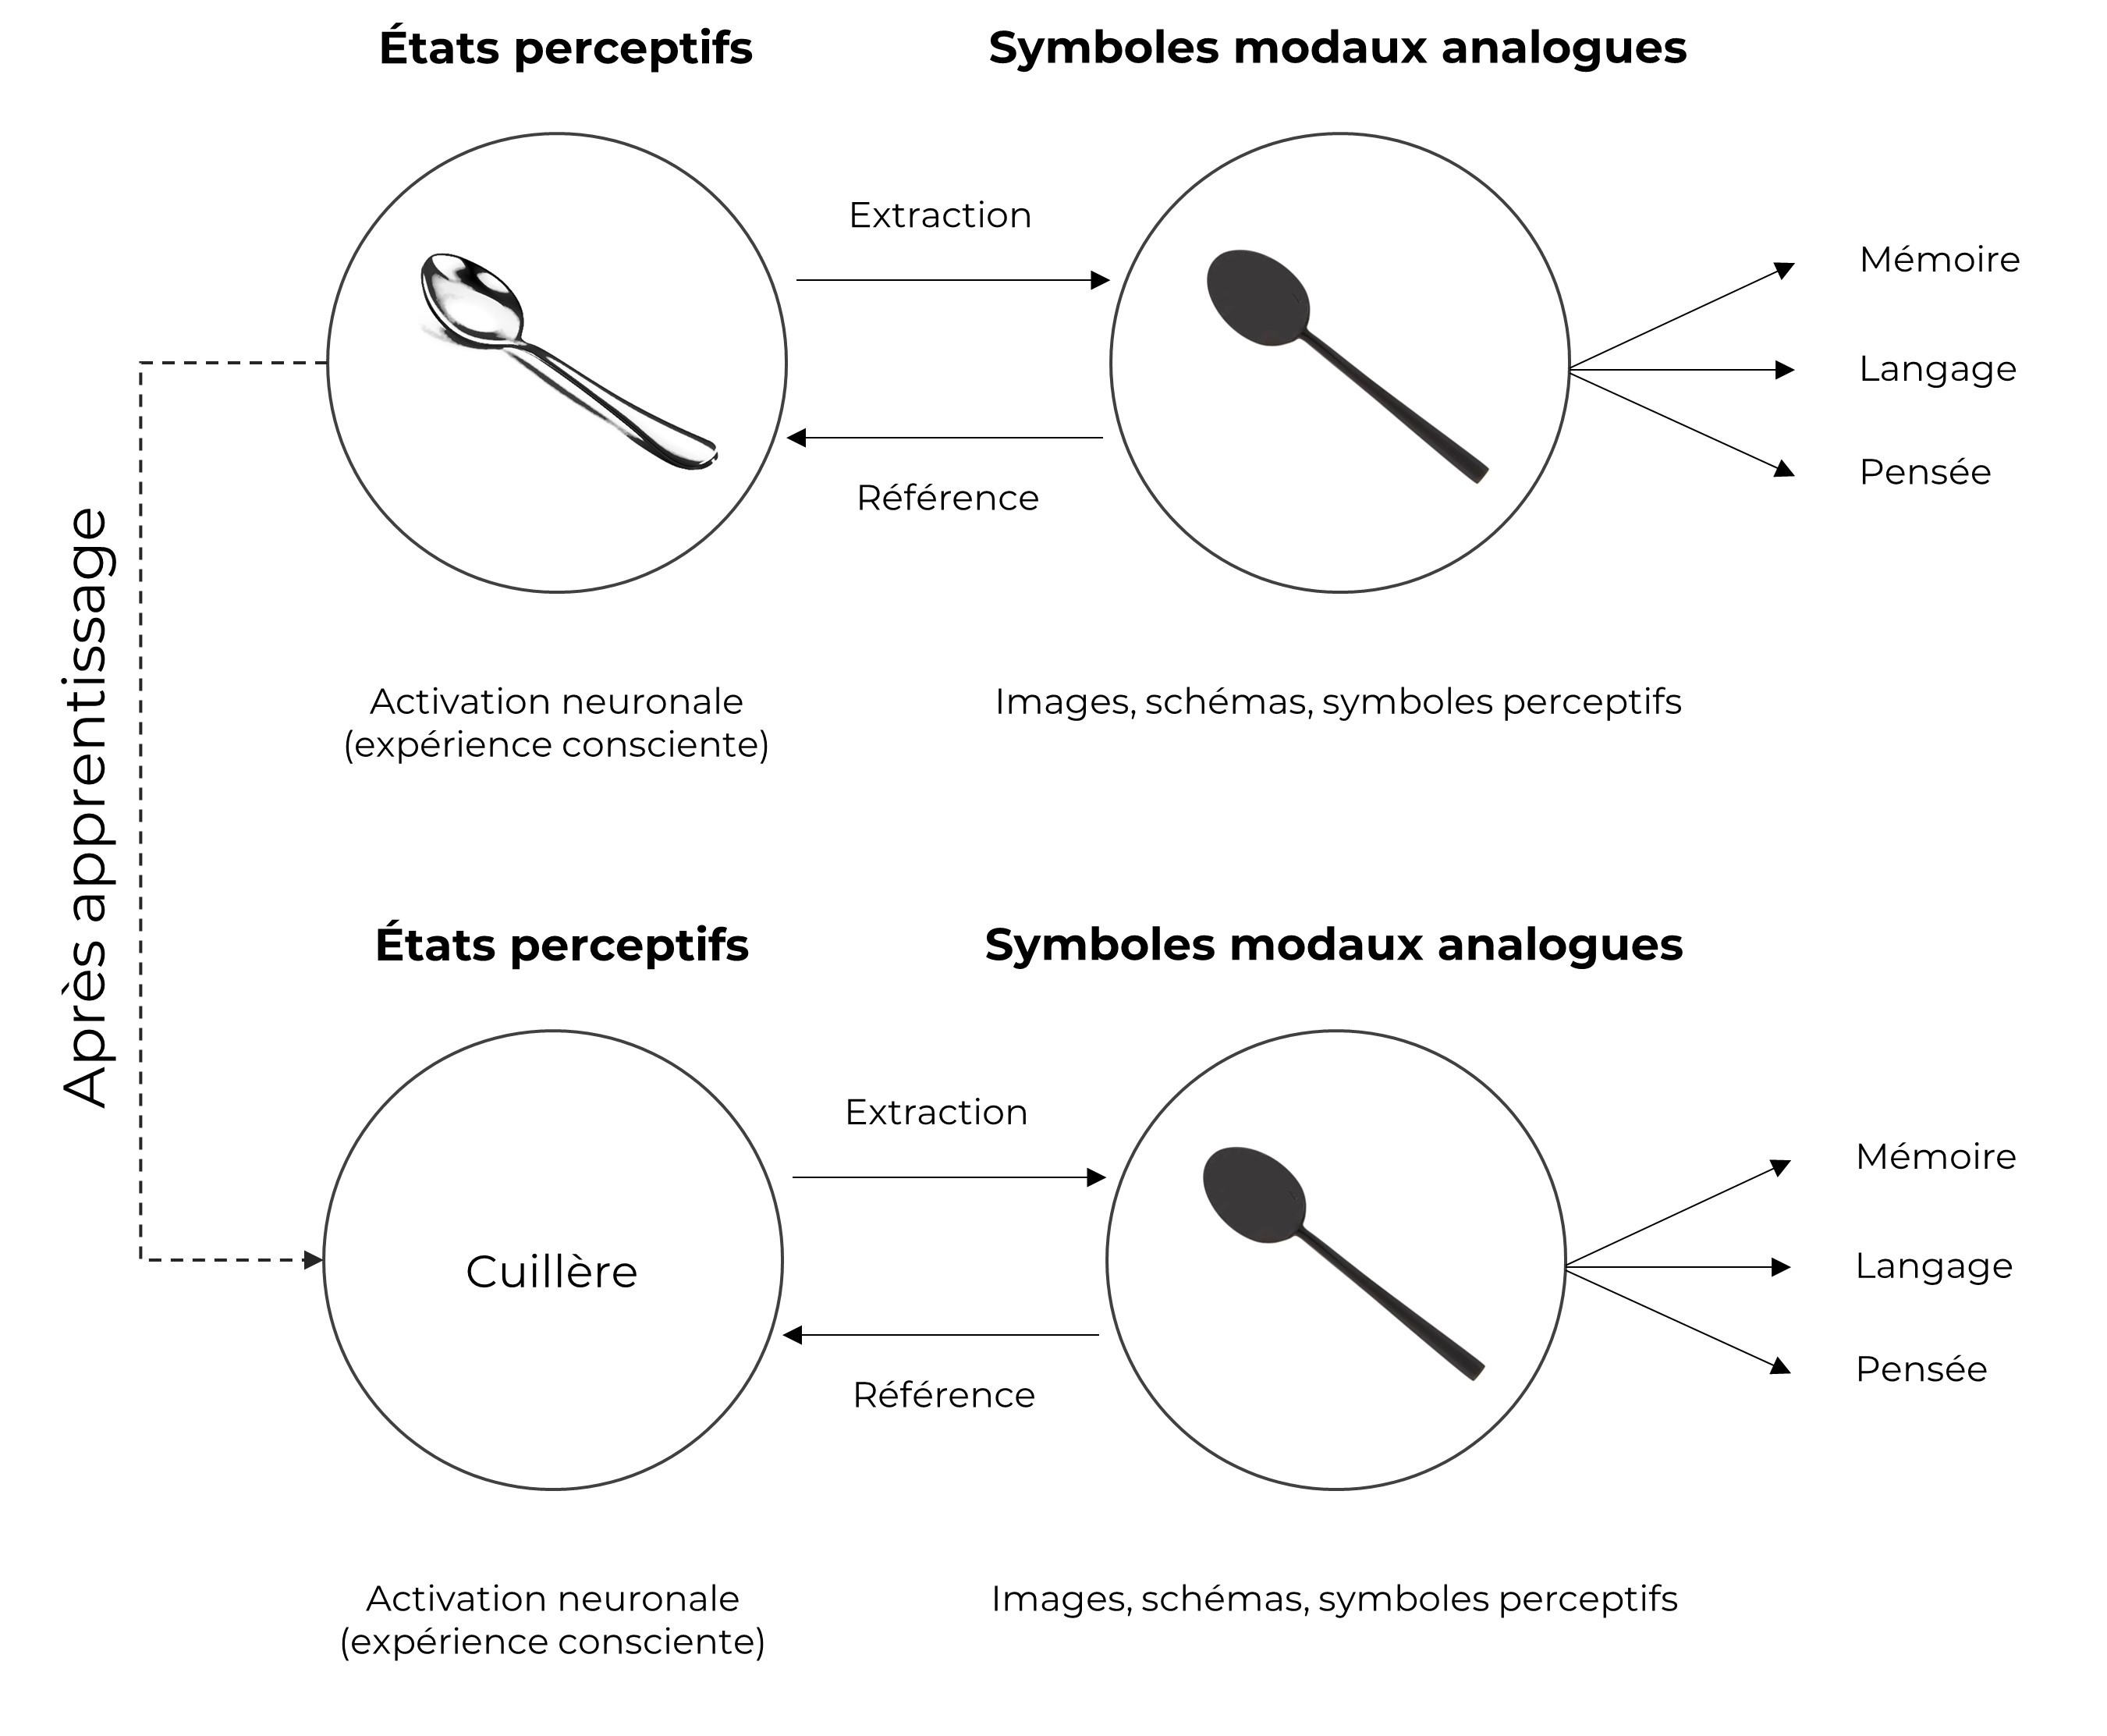
\includegraphics[width=1\linewidth]{figures/chap1-fig3} 

}

\caption{Proposition théorique des systèmes symboliques perceptifs (Barsalou, 1999) en alternative aux théories symboliques amodales (cf. Figure 1). Dans ce cadre, Barsalou propose que des ensembles d'états perceptifs dans les systèmes d'action et de perception seraient extraits et stockés en mémoire sous forme de symboles perceptifs, modaux. Selon Barsalou (1999), la 'structure interne des symboles' serait par essence incarnée, c'est-à-dire représentée dans le format spécifique à l'encodage. Dans ce cadre, les concepts ne seraient pas abstraits et amodaux mais ancrés dans les systèmes sensorimoteurs et émotionnels plutôt que dans les informations linguistiques. Barsalou (2008) considère les mots comme des \textit{pointeurs} dont la fonction est de réactiver ou de \textit{simuler} des états sensoriels liés à des objets ou des situations. Dans ce cadre, au fur et à mesure des interactions avec un concept, ici avec l'objet \textit{cuillère}, la présentation du mot 'cuillère' induirait la même activation corticale que la présentation de l'objet \textit{cuillère}.}\label{fig:chap1-fig3}
\end{figure}

En parallèle, \protect\hyperlink{ref-pulvermuller_concept_1996}{Pulvermüller \& Mohr} (\protect\hyperlink{ref-pulvermuller_concept_1996}{1996}) proposent d'expliquer l'ancrage conceptuel dans les systèmes moteurs et perceptifs à partir du principe d'apprentissage hebbien (\protect\hyperlink{ref-hebb_organization_1949}{Hebb, 1949}). Cette règle d'apprentissage par corrélation implique que des ensembles de neurones interconnectés et fréquemment coactivés vont renforcer leurs connexions mutuelles, pour former in fine une unité fonctionnelle de cellules neuronales : un réseau (\protect\hyperlink{ref-hebb_organization_1949}{Hebb, 1949}). L'activation de certaines parties du réseau suffirait à activer l'unité dans son ensemble de façon rapide et automatique. Selon \protect\hyperlink{ref-pulvermuller_words_1999}{Pulvermüller} (\protect\hyperlink{ref-pulvermuller_words_1999}{1999}), l'apprentissage hebbien permet d'expliquer comment l'activité corrélée entre un mot et l'expérience sensorimotrice concomitante conduirait à la formation de réseaux sémantiques largement distribués, comprenant des régions corticales impliquées dans l'action et la perception (\protect\hyperlink{ref-pulvermuller_words_1999}{Pulvermüller, 1999}; \protect\hyperlink{ref-pulvermuller_active_2010}{Pulvermüller \& Fadiga, 2010}; \protect\hyperlink{ref-pulvermuller_concept_1996}{Pulvermüller \& Mohr, 1996}).

Ces théories reposent sur un principe commun : les concepts seraient représentés dans de larges assemblées neuronales distribuées sur l'ensemble du cerveau, comprenant des structures motrices, sensorielles et émotionnelles (e.g., \protect\hyperlink{ref-barsalou_grounded_2008}{Barsalou, 2008a}, \protect\hyperlink{ref-barsalou_perceptual_1999}{1999}; \protect\hyperlink{ref-borghi_challenge_2017}{Borghi et al., 2017}; \protect\hyperlink{ref-boulenger_grasping_2009}{Boulenger et al., 2009}; \protect\hyperlink{ref-ghio_decoding_2016}{Ghio et al., 2016}; \protect\hyperlink{ref-pulvermuller_words_1999}{Pulvermüller, 1999}; \protect\hyperlink{ref-pulvermuller_active_2010}{Pulvermüller \& Fadiga, 2010}; \protect\hyperlink{ref-pulvermuller_concept_1996}{Pulvermüller \& Mohr, 1996}). Notons qu'à partir de maintenant nous nous détacherons du terme \emph{symbole}, auquel nous préférerons celui de concept.

\hypertarget{pred}{%
\subsubsection{Arguments empiriques en faveur d'un traitement sémantique incarné}\label{pred}}

Les premiers arguments empiriques à l'appui des théories incarnées du traitement conceptuel se sont avant tout focalisés sur les concepts dits concrets, à savoir des concepts désignant des actions (e.g., \emph{cueillir} , \protect\hyperlink{ref-glenberg_grounding_2002}{Glenberg \& Kaschak, 2002}), des objets observables et/ou manipulables (e.g., \emph{feuilles}, \protect\hyperlink{ref-pecher_verifying_2003}{Pecher et al., 2003}). Il existe un nombre important d'exemples faisant état d'interactions entre le langage et le système moteur, et l'existence de telles interactions ne fait plus débat. Par exemple, \protect\hyperlink{ref-damasio_time-locked_1989}{A. R. Damasio} (\protect\hyperlink{ref-damasio_time-locked_1989}{1989b}) a montré que des tâches de récupération de verbes activent des aires cérébrales traditionnellement associées au contrôle moteur. \protect\hyperlink{ref-chao_representation_2000}{Chao \& Martin} (\protect\hyperlink{ref-chao_representation_2000}{2000}) ont montré que la perception visuelle d'objets manipulables, ou la seule lecture de leur nom, suffisait à activer des aires cérébrales traditionnellement associées au contrôle moteur. Des activations spécifiques aux modalités d'interactions avec les objets sont aussi rapportées ; le traitement de mots désignant des objets caractérisés par des informations visuelles, olfactives, gustatives, et auditives se traduit par l'activation des aires sensorielles correspondantes (e.g., \protect\hyperlink{ref-barros-loscertales_reading_2012}{Barrós-Loscertales et al., 2012}; \protect\hyperlink{ref-kiefer_sound_2008}{Kiefer et al., 2008}). Par exemple, la compréhension d'un mot d'action comme \emph{courir} active le cortex moteur primaire alors que la compréhension de mots associés à des expériences plus visuelles comme \emph{lune} active les aires visuelles (e.g., \protect\hyperlink{ref-hauk_somatotopic_2004}{Hauk et al., 2004}; \protect\hyperlink{ref-pulvermuller_distributed_2009}{Pulvermüller et al., 2009}). Un dernier exemple intéressant est l'étude de \protect\hyperlink{ref-mathot_pupillary_2017}{Mathôt et al.} (\protect\hyperlink{ref-mathot_pupillary_2017}{2017}) où la présentation (visuelle ou auditive) de mots désignant différents degrés de luminosité suffisait à induire les réflexes pupillaires associés, à savoir une dilatation pupillaire pour les mots évoquant l'obscurité (e.g., \emph{nuit}, \emph{sombre}) et une contraction pupillaire pour les mots évoquant la luminosité (e.g., \emph{jour}, \emph{soleil}).

Pour \protect\hyperlink{ref-pulvermuller_brain_2005}{Pulvermüller} (\protect\hyperlink{ref-pulvermuller_brain_2005}{2005}), si de tels circuits neuronaux distribués - formés à partir d'informations corrélées liées à l'action et à la perception - fournissent le substrat neurobiologique du langage, alors plusieurs prédictions pouvaient être formulées concernant le traitement de verbes d'action. Premièrement, toute forme d'interaction avec un mot ou un concept désignant une action devrait activer les structures corticales communément impliquées dans le contrôle et l'exécution de cette action, et ce en respectant la somatotopie corticale. Deuxièmement, en raison de la rapidité de conduction du signal nerveux le long des axones, la présentation de mots d'actions (entendus ou lus) devrait provoquer l'activation rapide de l'ensemble du réseau sémantique auquel ce mot appartient, dont des neurones sensorimoteurs. Troisièmement, ce principe d'activation rapide devrait être automatique, dans le sens où il ne devrait pas être dépendant de l'attention des participant·e·s sur le contenu sémantique du stimulus verbal. Enfin, toute modification de l'activité des structures motrices et prémotrices devrait avoir un impact sur le traitement des mots d'action, de façon spécifique à la catégorie d'action. Il existe toute une série de travaux qui étayent ces prédictions que nous aborderons dans les sections suivantes à la lumière des discussions qu'ils ont engagées.

\hypertarget{challenge}{%
\subsubsection{Limites imputées aux propositions théoriques incarnés}\label{challenge}}

Dans cette section, nous présenterons et discuterons les données empiriques à l'appui des prédictions que nous venons de mentionner. Ces données soulèvent en effet deux questions principales : celle de l'implication fonctionnelle causale des structures sensorimotrices dans le traitement conceptuel, et celle de l'ancrage des concepts abstraits (e.g., \emph{temps}, \emph{liberté}) pour lesquels l'expérience sensorimotrice ne va pas de soi.

\hypertarget{epi}{%
\paragraph{Implication causale ou épiphénomènale des structures corticales sensorimotrices}\label{epi}}

L'exemple typiquement cité pour étayer la première prédiction de \protect\hyperlink{ref-pulvermuller_brain_2005}{Pulvermüller} (\protect\hyperlink{ref-pulvermuller_brain_2005}{2005}) est l'étude en IRMf de \protect\hyperlink{ref-hauk_somatotopic_2004}{Hauk et al.} (\protect\hyperlink{ref-hauk_somatotopic_2004}{2004}). Dans cette étude, les auteur·e·s rapportent que la lecture passive de mots d'action associés au pied, à la main, ou à la bouche (e.g., \emph{shooter}, \emph{cueillir}, \emph{lécher}), active de façon somatotopique les cortex moteur et prémoteur (pour des exemples similaires, voir également \protect\hyperlink{ref-carota_body-part-specific_2012}{Carota et al., 2012}; \protect\hyperlink{ref-de_lafuente_language_2004}{Lafuente \& Romo, 2004}; \protect\hyperlink{ref-tettamanti_listening_2005-1}{Tettamanti et al., 2005}). Cette étude est cohérente avec les notions selon lesquelles la compréhension de verbes d'action réutilise des structures corticales en charge de l'action motrice, et avec l'idée d'une activation fonctionnelle (causale) et automatique du système moteur (\protect\hyperlink{ref-pulvermuller_brain_2005}{Pulvermüller, 2005}).

Le postulat d'une implication fonctionnelle et automatique de structures sensorimotrices pour le langage et la compréhension a été vivement contesté (e.g., \protect\hyperlink{ref-mahon_critical_2008}{Mahon \& Caramazza, 2008}; \protect\hyperlink{ref-ritchie_massive_2010}{Ritchie \& Carruthers, 2010}). Une question centrale est de savoir si l'implication des aires dites de bas niveau lors du traitement sémantique est nécessaire ou s'il s'agit d'un épiphénomène. Autrement dit, est-ce que les aires sensorimotrices sont causalement impliquées dans le traitement sémantique, ou est-ce que leur activation n'est qu'un effet secondaire ? Cette limite, aussi appelée « l'objection de la portée » (\protect\hyperlink{ref-pecher_abstract_2011}{Pecher et al., 2011}), interroge sur l'implication nécessaire et suffisante des structures sensorimotrices dans l'accès sémantique. En effet, pouvons-nous affirmer que l'activation de l'aire occipitale ventrale (associée au traitement de la couleur, e.g., \protect\hyperlink{ref-lueck_colour_1989}{Lueck et al., 1989}) à la vue d'une orange implique que cette aire est nécessaire à sa reconnaissance ? Comme nous sommes capables de reconnaitre le fruit sur la base d'une image en noir et blanc, il semble évident que la réponse est non (\protect\hyperlink{ref-cayol_why_2020}{Cayol \& Nazir, 2020}). L'information de couleur ne servirait qu'à enrichir le percept du fruit (\protect\hyperlink{ref-mahon_critical_2008}{Mahon \& Caramazza, 2008}). Dans ce cadre, les théoricien·ne·s de l'amodalité soutiennent que si l'activité sensorimotrice améliore le traitement sémantique, elle n'a aucun rôle causal dans la représentation et la compréhension de concepts.

Quant à la prédiction d'une activation automatique des structures sensorimotrices pour le traitement sémantique (\protect\hyperlink{ref-pulvermuller_brain_2005}{Pulvermüller, 2005}), les données obtenues n'étaient toujours pas convaincantes (e.g., \protect\hyperlink{ref-caramazza_cognitive_2006}{Caramazza \& Coltheart, 2006}; \protect\hyperlink{ref-mahon_critical_2008}{Mahon \& Caramazza, 2008}). Comme l'activation neuronale peut se propager dans les réseaux, observer une activation du système moteur consécutive au traitement sémantique de verbes d'action ne suffit pas à démontrer une implication causale du système moteur (elle serait là encore épiphénoménale) et encore moins automatique (e.g., \protect\hyperlink{ref-caramazza_cognitive_2006}{Caramazza \& Coltheart, 2006}; \protect\hyperlink{ref-mahon_critical_2008}{Mahon \& Caramazza, 2008}). Cet argument repose sur deux observations. Tout d'abord, la faible résolution temporelle de l'IRMf ne permet pas de tester le caractère automatique de l'activation des structures motrices et perceptives. Deuxièmement, plusieurs auteur·e·s ont émis des doutes quant à la fiabilité des observations (e.g., \protect\hyperlink{ref-tomasino_at_2013}{Tomasino \& Rumiati, 2013}; \protect\hyperlink{ref-watson_action_2013}{Watson et al., 2013}). Parmi eux, \protect\hyperlink{ref-tomasino_at_2013}{Tomasino \& Rumiati} (\protect\hyperlink{ref-tomasino_at_2013}{2013}) rapportent que les résultats physiologiques observés par \protect\hyperlink{ref-hauk_somatotopic_2004}{Hauk et al.} (\protect\hyperlink{ref-hauk_somatotopic_2004}{2004}) demeurent difficiles à répliquer, et ce, en dépit de la ressemblance des paradigmes utilisés, ce qui semble incompatible avec le postulat d'une activation automatique des structures sensorimotrices pour le traitement linguistique.

Si l'argument de la faible résolution temporelle de l'IRMf était pertinent, la réplication de ces effets topographiques (i.e., de la somatopopie motrice) en électroencéphalographie (EEG) et magnétoencéphalographie (MEG; e.g., \protect\hyperlink{ref-de_lafuente_language_2004}{Lafuente \& Romo, 2004}; \protect\hyperlink{ref-pulvermuller_brain_2005}{Pulvermüller, 2005}), qui n'ont pas ce défaut, ont fourni des arguments convaincants en faveur de l'hypothèse alternative, à savoir celle d'un traitement automatique. De même, ces études ont montré que l'activation topographique intervenait non seulement dès les étapes précoces du traitement lexical (dès 80 ms), mais aussi lorsque les participant·e·s ne portaient pas une attention volontaire et explicite sur les stimuli verbaux (e.g., \protect\hyperlink{ref-boulenger_subliminal_2008}{Boulenger et al., 2008}; \protect\hyperlink{ref-grisoni_somatotopic_2016}{Grisoni et al., 2016}; \protect\hyperlink{ref-pulvermuller_brain_2005-1}{Pulvermüller, Shtyrov, et al., 2005}; \protect\hyperlink{ref-shtyrov_automatic_2014}{Shtyrov et al., 2014}). Le traitement lexical se situant entre 150 et 400 ms (\protect\hyperlink{ref-friederici_towards_2002}{Friederici, 2002}), ce genre de données exclut l'hypothèse d'une activation épiphénoménale ou sans valeur fonctionnelle pour le traitement lexical (\protect\hyperlink{ref-shtyrov_automatic_2014}{Shtyrov et al., 2014}). Comme prédit par \protect\hyperlink{ref-pulvermuller_brain_2005}{Pulvermüller} (\protect\hyperlink{ref-pulvermuller_brain_2005}{2005}), ces résultats suggèrent plutôt une activation rapide (deuxième prédiction) et automatique (troisième prédiction) des structures motrices pour la compréhension de verbes d'action.

Concernant la dernière prédiction, à savoir qu'une modulation de l'activité motrice corticale devrait influencer le traitement des verbes d'action, des effets facilitateurs ou inhibiteurs du traitement lexical ont été obtenus en modulant transitoirement l'activité du cortex moteur. Par exemple, en utilisant la stimulation magnétique transcranienne, des auteur·e·s ont mis en évidence une facilitation du traitement de verbes d'actions liés aux mouvements des membres inférieurs ou supérieurs lors d'une stimulation des structures motrices en charge du contrôle et de l'exécution de ces mouvements (\protect\hyperlink{ref-pulvermuller_functional_2005}{Pulvermüller, Hauk, et al., 2005}). À l'inverse, des effets d'amorçage physiologique ont également été rapportés dans une étude où la présentation de mots d'actions liés au visage ou à la jambe a facilité le traitement de verbes associés à ces effecteurs (\protect\hyperlink{ref-grisoni_somatotopic_2016}{Grisoni et al., 2016}). Ces études d'amorçage physiologiques apportent des arguments solides en faveur d'une implication causale (plutôt qu'épiphénoménale), rapide, et automatique des structures motrices pour la compréhension de verbes d'actions.

Un dernier exemple intéressant pour notre exposé sur les relations entre compréhension et structures motrices est l'effet de compatibilité action-phrase (désormais ACE pour action compatibility effect) rapporté par \protect\hyperlink{ref-glenberg_grounding_2002}{Glenberg \& Kaschak} (\protect\hyperlink{ref-glenberg_grounding_2002}{2002}). Dans cette étude, on demande à des participant·e·s de faire des jugements de grammaticalité sur des phrases en produisant des mouvements du bras vers l'avant (éloignement) ou vers leur corps (rapprochement). Les phrases d'intérêt décrivent des actions de rapprochement, comme « met la cuillère dans ta bouche », ou d'éloignement, comme « ferme le tiroir ». L'ACE se traduit par une interaction entre les deux conditions, à savoir des temps de réactions plus longs lorsque la phrase décrit un mouvement opposé au mouvement à réaliser pour répondre (voir cependant l'échec de réplication multi-laboratoire de \protect\hyperlink{ref-morey_pre-registered_2021}{Morey et al., 2021} dans laquelle 18 laboratoires ne répliquent pas cet effet).

Ces effets de congruence ne sont pas anecdotiques. En effet, si l'on suit le raisonnement établi par \protect\hyperlink{ref-sternberg_discovery_1969}{Sternberg} (\protect\hyperlink{ref-sternberg_discovery_1969}{1969}), les interactions observées entre deux facteurs manipulés impliquent une composante partagée entre les deux processus, ici le mouvement du bras et l'accès sémantique lors de la tâche de jugement de grammaticalité. Ainsi, de tels effets de congruence montrent que l'utilisation de ressources neuronales dans une tâche donnée les rend moins disponibles pour d'autres tâches et apportent un argument empirique fort en faveur d'une utilisation de structures corticales communes.

\hypertarget{le-challenge-des-concepts-abstraits}{%
\paragraph{Le challenge des concepts abstraits}\label{le-challenge-des-concepts-abstraits}}

De nombreux auteur·e·s reconnaissent aujourd'hui l'efficacité des théories incarnées pour rendre compte de la représentation conceptuelle, comme le témoigne le nombre considérable d'études faisant état de l'implication causale des structures motrices et perceptives pour le traitement de concepts concrets (e.g., \protect\hyperlink{ref-barros-loscertales_reading_2012}{Barrós-Loscertales et al., 2012}; \protect\hyperlink{ref-boulenger_subliminal_2008}{Boulenger et al., 2008}, \protect\hyperlink{ref-boulenger_when_2012}{2012}, \protect\hyperlink{ref-boulenger_cross-talk_2006}{2006}; \protect\hyperlink{ref-pulvermuller_functional_2005}{Pulvermüller, Hauk, et al., 2005}; \protect\hyperlink{ref-willems_functional_2011}{Willems et al., 2011}; pour revue voir \protect\hyperlink{ref-pulvermuller_neural_2018}{Pulvermüller, 2018a}). Cependant, si le sens d'un mot ou d'un concept est représenté dans un format modal, c'est-à-dire dans un format qui contient des informations issues d'interactions perceptives, motrices, et émotionnelles, comment ces théories peuvent-elles rendre compte de concepts dénués de propriétés tangibles comme les concepts de \emph{liberté} ou de \emph{temps} ? Cette question est ce qui constitue la faiblesse des théories incarnées selon \protect\hyperlink{ref-dove_beyond_2009}{Dove} (\protect\hyperlink{ref-dove_beyond_2009}{2009}; \protect\hyperlink{ref-mahon_what_2015}{Mahon, 2015}; voir aussi \protect\hyperlink{ref-mahon_critical_2008}{Mahon \& Caramazza, 2008}). Comme l'individu ne manipule pas directement -- par l'action ou la perception -- les concepts abstraits, il n'est pas évident de savoir comment de tels concepts peuvent être représentés par des simulations sensorimotrices. Notons que \protect\hyperlink{ref-dove_beyond_2009}{Dove} (\protect\hyperlink{ref-dove_beyond_2009}{2009}) ne nie pas les éléments empiriques en faveur de processus incarnés, il considère en revanche qu'ils ne sont applicables qu'à l'étude des concepts concrets hautement « imageables », comme \emph{orange} ou \emph{cuillère.} En s'appuyant sur la théorie du double codage (\protect\hyperlink{ref-paivio_dual_1991}{Paivio, 1991}), Dove soutient que les concepts abstraits comme les concepts de \emph{liberté} ou de \emph{temps} seraient nécessairement amodaux (i.e., désincarnés).

Intuitivement, il semble plus pertinent d'adopter une approche symbolique amodale pour appréhender les concepts abstraits. Par exemple, le concept de \emph{temps} renvoie à une entité immatérielle. Il n'existe aucun stimulus spécifique au temps, que nos récepteurs sensoriels seraient capables de détecter et nous ne disposons pas d'organe dédié spécifiquement au traitement des informations temporelles (e.g., \protect\hyperlink{ref-evans_structure_2003}{Evans, 2003}; \protect\hyperlink{ref-grondin_physical_2001}{Grondin, 2001}). Il semble alors logique de se demander comment pareil concept pourrait s'ancrer par son interaction avec l'expérience sensorimotrice si par définition il en est dépourvu. Si nous avons des représentations amodales pour les concepts abstraits, alors le problème de l'ancrage resurgit
(\protect\hyperlink{ref-pecher_abstract_2011}{Pecher et al., 2011}, cf.~encart \ref{symbol} pour le problème de l'ancrage).

Les tenants des théories amodales mettent en avant l'importance pour toute théorie du langage de pouvoir rendre compte de la façon dont un individu peut acquérir, manipuler, et accéder au sens des concepts abstraits (e.g., \protect\hyperlink{ref-dove_beyond_2009}{Dove, 2009}; \protect\hyperlink{ref-mahon_critical_2008}{Mahon \& Caramazza, 2008}). Notons que les théories incarnées les rejoignent sur ce point, mais insistent sur le fait que les théories amodales n'en semblent pas non plus capables en ne fournissant aucune alternative convaincante pour rendre compte des concepts abstraits (\protect\hyperlink{ref-lupyan_language_2018}{Lupyan \& Winter, 2018}). Une réponse pertinente - que nous adoptons dans ce manuscrit - est celle fournie par le modèle des circuits d'action-perception (e.g., \protect\hyperlink{ref-pulvermuller_neural_2018}{Pulvermüller, 2018a}, \protect\hyperlink{ref-pulvermuller_how_2013}{2013}; \protect\hyperlink{ref-pulvermuller_active_2010}{Pulvermüller \& Fadiga, 2010}) développé sur le principe de réutilisation neuronale, et que nous détaillerons dans le chapitre \ref{chap2}. Plus précisément, nous appliquerons ce modèle à l'étude du concept abstrait de \emph{temps}.

\newpage

\begin{vplace}[1]

\begin{summary}{Résumé du Chapitre\getcurrentref{chapter}}{\chaptercolor}

Dans ce chapitre, nous avons proposé un aperçu des théories cognitivistes, philosophiques et neuroscientifiques en lien avec le traitement conceptuel. Cet aperçu nous a permis d’examiner les limites des conceptions modulaires et amodales du traitement sémantique, avant d’aborder la proposition de réponses apportée par les conceptions incarnées du langage. En particulier, nous avons mis l’accent sur la théorie de réutilisation neuronale (Anderson, 2010; 2014), qui propose d’expliquer comment le corps et les ressources disponibles se trouvent intrinsèquement et fonctionnellement liés à la cognition. En accord avec les théories de réutilisation neuronale (Anderson, 2010; 2014; Gallese, 2008; Parkinson \& Wheatley, 2013), nous avons proposé que certaines structures et certains mécanismes de base, comme ceux du système moteur, sont réutilisés à un niveau supérieur par le langage. En ce sens, nous pouvons parler d'ancrage du langage.\\

Enfin, nous avons établi que si de nombreux arguments empiriques appuient le postulat de processus incarnés pour la représentation des concepts dits concrets, la mesure dans laquelle l’utilisation de structures sensorimotrices jouent un rôle fonctionnel pour le traitement conceptuel est encore largement débattue. En effet, certains considèrent que l’implication des structures sensorimotrices ne serait qu’un épiphénomène et manque d’étayage. Cette question est d’autant plus importante dans le cadre des concepts abstraits, dénués de propriétés tangibles avec lesquelles interagir, qui représentent pour certain·e·s auteur·e·s un argument suffisant à l’encontre des théories incarnées du langage.\\

Dans le chapitre \ref{chap2}, nous discuterons des éléments théoriques et empiriques disponibles pour appréhender i) les contours de ce qui caractérise un concept comme abstrait, ii) l’état de l’art empirique en faveur d’une représentation distribuée et plurimodale pour les concepts abstraits, iii) les propositions théoriques incarnées pour expliquer les mécanismes qui rendent possible l’ancrage des concepts abstraits. Nous considérerons le concept abstrait de temps comme cas d’étude pour approfondir les questions encore non résolues que nous aborderons dans les chapitres expérimentaux de ce manuscrit.

\end{summary}

\end{vplace}

\changechaptercolor{hokusai2}

\hypertarget{chap2}{%
\chapter{Traitement des concepts abstraits temporels}\label{chap2}}

\epigraph{"The fact is that an idea and its meaning are based on systems that are equivalent for associative purposes. The practical value of a word is that it, a comparatively simple movement system, has the same tendencies to excite other movement systems that is possessed by what may be a much more complex movement system, its meaning."}{Washburn M. F. (1916, p.219)}

\initial{L}a représentation des concepts abstraits a fait l'objet de vifs débats, principalement parce que ces derniers ne semblaient pas se prêter à l'ancrage dans l'expérience sensorimotrice. Plusieurs propositions théoriques sont nées de ce débat, qui se différencient par le degré d'ancrage supposé (i.e., plus ou moins directement puisé dans l'expérience, voir par exemple \protect\hyperlink{ref-barsalou_grounded_2008}{Barsalou, 2008a}, \protect\hyperlink{ref-barsalou_perceptual_1999}{1999}; \protect\hyperlink{ref-lakoff_philosophy_1999}{Lakoff \& Johnson, 1999}; \protect\hyperlink{ref-pulvermuller_words_1999}{Pulvermüller, 1999}, \protect\hyperlink{ref-pulvermuller_neurobiological_2018}{2018b}, \protect\hyperlink{ref-pulvermuller_case_2018}{2018c}). Dans un premier temps, ce chapitre présentera et discutera de ces propositions théoriques, et cadre théorique adopté dans ce manuscrit (i.e., le modèle des circuits d'action-perception). Dans un second temps, nous verrons comment ce cadre théorique peut s'appliquer à l'étude des concepts abstraits temporels. Enfin, nous terminerons avec un aperçu des problématiques qui seront abordées dans les chapitres expérimentaux.

\hypertarget{defa}{%
\section{Les concepts abstraits : une perspective multidimensionnelle}\label{defa}}

La capacité de l'individu à transcender le monde physique pour se former une représentation de concepts comme \emph{liberté}, \emph{astrophysique}, ou \emph{temps}, est considérée comme l'une des plus sophistiquées et essentielles pour la cognition humaine (e.g., \protect\hyperlink{ref-borghi_words_2014}{Borghi \& Binkofski, 2014}; \protect\hyperlink{ref-desai_multifaceted_2018}{Desai et al., 2018}; \protect\hyperlink{ref-villani_varieties_2019}{Villani et al., 2019}). Plus que le reflet d'une habileté sophistiquée, les concepts abstraits seraient omniprésents, occupant plus de 60\% de notre vocabulaire quotidien (e.g., \protect\hyperlink{ref-brysbaert_moving_2009}{Brysbaert \& New, 2009}; \protect\hyperlink{ref-lupyan_language_2018}{Lupyan \& Winter, 2018}). Les nombreuses discussions au sujet des concepts abstraits ont avant tout porté sur la différence entre les concepts tels que \emph{liberté}, \emph{temps}, ou \emph{astrophysique}, en opposition à \emph{cuillère}, \emph{orange}, ou \emph{courir.} En somme, qu'est-ce que cela implique de dire que le concept de \emph{temps} est plus abstrait que le concept de \emph{cuillère} ?

Pour une grande partie des études sur le système sémantique, les concepts concrets, comme \emph{cuillère}, \emph{orange}, ou encore \emph{marcher} désignent des objets manipulables et/ou observables par les systèmes sensoriels, et/ou des actions exécutables par le système moteur (e.g., \protect\hyperlink{ref-desai_multifaceted_2018}{Desai et al., 2018}; \protect\hyperlink{ref-paivio_abstractness_1965}{Paivio, 1965}; \protect\hyperlink{ref-villani_varieties_2019}{Villani et al., 2019}). En revanche, les concepts abstraits comme \emph{temps}, \emph{passé}, ou \emph{futur}, désignent une catégorie de mots dénués de référents physiques immédiat -- ils ne sont ni physiquement ni spatialement contraints -- et qui, par définition, ne peuvent pas être expérimentés par les systèmes sensoriels et moteurs (e.g., \protect\hyperlink{ref-dijkstra_embodied_2014}{Dijkstra et al., 2014}; \protect\hyperlink{ref-paivio_abstractness_1965}{Paivio, 1965}, \protect\hyperlink{ref-paivio_imagery_1971}{1971}). Cette définition est peu satisfaisante car les concepts abstraits sont définis négativement, à partir de propriétés qu'ils ne possèdent pas, en comparaison aux concepts concrets (e.g., \protect\hyperlink{ref-barsalou_moving_2018}{Barsalou et al., 2018}; \protect\hyperlink{ref-borghi_words_2014}{Borghi \& Binkofski, 2014}; \protect\hyperlink{ref-desai_multifaceted_2018}{Desai et al., 2018}).

Pour une définition positive des concepts abstraits, nous adoptons celle proposée par Borghi et Binkofski (2014), à savoir que les concepts abstraits, qui n'ont généralement pas d'objet unique comme référent, seraient davantage détachés des entités physiques et des modalités sensorielles (e.g, \protect\hyperlink{ref-barsalou_abstraction_2003}{Barsalou, 2003}; \protect\hyperlink{ref-pecher_situating_2005}{Barsalou \& Wiemer-Hastings, 2005}), pour être davantage liés aux états intéroceptifs (e.g., \protect\hyperlink{ref-connell_interoception_2018}{Connell et al., 2018}; \protect\hyperlink{ref-villani_sensorimotor_2021}{Villani et al., 2021}) et émotionnels (e.g., \protect\hyperlink{ref-kousta_representation_2011}{Kousta et al., 2011}; \protect\hyperlink{ref-ponz_emotion_2014}{Ponz et al., 2014}; \protect\hyperlink{ref-ziegler_words_2018}{Ziegler et al., 2018}). Enfin, ils feraient référence à des situations nombreuses et variables (\protect\hyperlink{ref-pulvermuller_case_2018}{Pulvermüller, 2018c}).

Bien qu'historiquement les concepts abstraits et concrets aient été considérés comme des entités dichotomiques (\protect\hyperlink{ref-paivio_abstractness_1965}{Paivio, 1965}), les efforts fournis ces dix dernières années montrent que la distinction entre ces deux classes de concepts n'est pas si tranchée (e.g., \protect\hyperlink{ref-borghi_words_2014}{Borghi \& Binkofski, 2014}; \protect\hyperlink{ref-della_rosa_beyond_2010}{Della Rosa et al., 2010}; \protect\hyperlink{ref-desai_multifaceted_2018}{Desai et al., 2018}; \protect\hyperlink{ref-lakhzoum_semantic_2021}{Lakhzoum et al., 2021}; \protect\hyperlink{ref-villani_sensorimotor_2021}{Villani et al., 2021}). Les données les plus récentes en psycholinguistique suggèrent qu'à la place d'une distinction unidimensionnelle (i.e., par le degré de concrétude / abstraction), les concepts se distribueraient de manière continue dans un espace dans lequel les concepts plus concrets et plus abstraits pourraient être représentés le long de plusieurs continuums (\protect\hyperlink{ref-fini_articulatory_2021}{Fini et al., 2021}).

Ces observations s'appliquent également à l'intérieur même de la catégorie des concepts abstraits. Loin d'être un tout unitaire, les concepts abstraits seraient constitués de différents sous-types de concepts, chacun représenté par de multiples dimensions (pour revue voir \protect\hyperlink{ref-conca_multidimensionality_2021}{Conca et al., 2021}). Ces dimensions seraient plus ou moins pertinentes selon le type de concept impliqué, comprenant à des degrés divers des informations situationnelles, des expériences sensorimotrices, intéroceptives, ou encore émotionnelles (e.g., \protect\hyperlink{ref-desai_multifaceted_2018}{Desai et al., 2018}; \protect\hyperlink{ref-ponz_emotion_2014}{Ponz et al., 2014}; \protect\hyperlink{ref-silva_emotions_2012}{Silva et al., 2012}; \protect\hyperlink{ref-villani_varieties_2019}{Villani et al., 2019}). À titre d'exemple, \protect\hyperlink{ref-villani_varieties_2019}{Villani et al.} (\protect\hyperlink{ref-villani_varieties_2019}{2019}) ont demandé à des participant·e·s d'évaluer 425 mots désignant des concepts abstraits sur 15 dimensions (e.g., imageabilité, disponibilité contextuelle, intéroception, perception, etc.). Des analyses en cluster ont montré que les concepts abstraits étaient mieux représentés par quatre sous-types de concepts plutôt qu'un seul, à savoir : i) des concepts physiques, spatio-temporels, et quantitatifs (e.g., \emph{masse}, \emph{espace}, \emph{fin}, \emph{nombre}) plus concrets, davantage représentés par des aspects sensorimoteurs, en opposition aux ii) concepts philosophiques et spirituels, plus abstraits (e.g., \emph{destin}), iii) des concepts de soi et sociaux (e.g., \emph{générosité}) ancrés à la fois dans des entités perceptives et intéroceptives, et enfin iv) des concepts liés aux états émotionnels et internes (e.g., \emph{amour}, \emph{liberté}, voir aussi \protect\hyperlink{ref-desai_multifaceted_2018}{Desai et al., 2018}; \protect\hyperlink{ref-harpaintner_grounding_2020}{Harpaintner et al., 2020}; et \protect\hyperlink{ref-conca_multidimensionality_2021}{Conca et al., 2021} pour revue récente). Face à cette diversité, \protect\hyperlink{ref-barsalou_moving_2018}{Barsalou et al.} (\protect\hyperlink{ref-barsalou_moving_2018}{2018}) suggèrent d'abandonner la classification des concepts abstraits vs.~concrets. En alternative, comme les concepts émergent du traitement de situations, il parait plus adéquat de les étudier dans leur contexte d'apparition (\protect\hyperlink{ref-barsalou_moving_2018}{Barsalou et al., 2018}).

En résumé, les concepts abstraits ne sont pas tous abstraits de la même manière. Ils varient selon différentes dimensions, peuvent avoir plusieurs degrés d'abstraction et être ancrés sur une grande variété d'expériences : certaines impliquant davantage le corps et d'autres les états internes et émotionnels (e.g., \protect\hyperlink{ref-desai_multifaceted_2018}{Desai et al., 2018}; \protect\hyperlink{ref-villani_varieties_2019}{Villani et al., 2019}). Dans la section suivante, nous verrons quelques arguments empiriques qui appuient le postulat de processus incarnés pour les concepts abstraits. Dans un second temps, nous discuterons de plusieurs propositions théoriques (incarnées) pour expliquer par quels mécanismes de tels concepts peuvent être ancrés à partir d'expériences sensorimotrices dans l'environnement.

\hypertarget{incarnation}{%
\section{L'incarnation des concepts abstraits}\label{incarnation}}

\epigraph{"Leaving aside the highly philosophical question about their ontological status, it is undeniable that both abstract and concrete concepts are in fact concepts and therefore, in one sense, not in the world, where space and time apply, but rather 'in the mind'"}{Henningsen-Schomers, M. R. \& Pulvermüller, F. (2021, p.4)}

Ayant donné une définition des concepts abstraits, il convient maintenant de nous interroger sur la façon dont de tels concepts peuvent prendre racine dans un ensemble d'expériences sensorimotrices, émotionnelles, et intéroceptives. Si, comme nous venons de le voir, les concepts abstraits ne semblent pas incarnés sur des entités physiques perceptives et tangibles (à l'instar des concepts concrets), ils pourraient néanmoins être ancrés via une grande variété d'expériences qui comprennent à des degrés divers des situations, des états intéroceptifs, émotionnels, ou encore des relations entre les objets (e.g., \protect\hyperlink{ref-barsalou_grounded_2008}{Barsalou, 2008a}; \protect\hyperlink{ref-borghi_words_2014}{Borghi \& Binkofski, 2014}; \protect\hyperlink{ref-lakhzoum_semantic_2021}{Lakhzoum et al., 2021}). Dans cette optique, on suppose que de la même façon que le traitement de verbes d'actions réutilise des structures corticales motrices en respectant la somatotopie corticale (e.g., \protect\hyperlink{ref-hauk_somatotopic_2004}{Hauk et al., 2004}), ce qui suggère des activations spécifiques à la modalité, on devrait également observer des patterns d'activations corticales spécifiques à la modalité, lors du traitement de concepts abstraits.

À titre d'exemple, une méta-analyse de \protect\hyperlink{ref-desai_multifaceted_2018}{Desai et al.} (\protect\hyperlink{ref-desai_multifaceted_2018}{2018}) a montré que différents sous-types de concepts abstraits (i.e., liés au nombre, à l'émotion, à la moralité, ou à la théorie de l'esprit) engageaient des aires corticales communes mais aussi spécifiques à chaque sous-type de concept, suggérant des modalités d'encodage communes et spécifiques pour chaque sous-type. Plus récemment, une étude en IRMf a montré des activations spécifiques à la modalité pour le traitement de différents types de concepts abstraits ; les concepts abstraits en lien avec la vision, comme \emph{beauté}, engageaient spécifiquement des structures visuelles, alors que les concepts abstraits en lien avec l'action, comme \emph{combat}, activaient spécifiquement des structures motrices (\protect\hyperlink{ref-harpaintner_grounding_2020}{Harpaintner et al., 2020}; voir également \protect\hyperlink{ref-tschentscher_you_2012}{Tschentscher et al., 2012}; \protect\hyperlink{ref-wilson-mendenhall_contextual_2013}{Wilson-Mendenhall et al., 2013}, pour d'autres exemples). Enfin, des activations de structures motrices ont également été rapportées par une étude en IRMf où les participant·e·s devaient lire passivement des mots faisant référence à des concepts abstraits émotionnels (e.g., \emph{peur}) ou à des concepts concrets d'objets liés à des actions (e.g., \emph{scie}, \protect\hyperlink{ref-dreyer_abstract_2018}{Dreyer \& Pulvermüller, 2018}). Ces résultats suggèrent que l'utilisation de structures corticales motrices ne se limitent pas au traitement de concepts concrets mais s'étendrait au traitement de concepts abstraits.

Il est peu probable que ces activations spécifiques à la modalité d'encodage, y compris dans le système moteur, soit la conséquence de la propagation de l'activation dans les réseaux (i.e., activation épiphénomènale). Comme cette activation intervient automatiquement dès les étapes précoces du traitement, il est plus probable que ces activations fassent partie intégrante du processus d'accès sémantique précoce (\protect\hyperlink{ref-pulvermuller_neural_2018}{Pulvermüller, 2018a}). L'hypothèse alternative proposée par les théories incarnées semble offrir une explication neurobiologiquement plausible, à savoir que les processus de représentation sémantique seraient sous-tendus par de larges circuits distribués à la fois dans les aires multimodales atteignant des structures primaires comme les cortex sensorimoteurs et le système limbique (e.g., \protect\hyperlink{ref-dreyer_abstract_2018}{Dreyer \& Pulvermüller, 2018}).

Bien que ces résultats puissent être interprétés en faveur de processus incarnés pour la représentation des concepts, il n'existe toujours pas de consensus quant aux mécanismes qui les permettent (cf. \protect\hyperlink{ref-borghi_words_2014}{Borghi \& Binkofski, 2014}, pour discussion). En effet, le réel challenge qui existe aujourd'hui n'est pas de fournir des preuves empiriques en faveur d'activations de systèmes anciennement considérées comme de bas niveau ou sans rôle fonctionnel pour des processus aussi évolués que le langage. En revanche, il importe de comprendre par quels mécanismes ces structures se trouvent en réalité essentielles aux processus d'acquisition et de représentation conceptuelle. Dans ce sens, trois perspectives théoriques seront présentées et discutées dans la section suivante.

\hypertarget{lass}{%
\subsection{La théorie du langage et de la simulation : théorie LASS}\label{lass}}

Une première proposition théorique est la théorie du langage et de la simulation située (désormais LASS pour Language and Situated Simulation) proposée par \protect\hyperlink{ref-barsalou_language_2008}{Barsalou et al.} (\protect\hyperlink{ref-barsalou_language_2008}{2008}). Dérivée du principe de simulation (cf.~chapitre \ref{chap2}, \protect\hyperlink{ref-barsalou_perceptual_1999}{Barsalou, 1999}), la théorie LASS soutient également que les connaissances seraient représentées dans de multiples systèmes distribués (\protect\hyperlink{ref-barsalou_language_2008}{Barsalou et al., 2008}). Cette proposition théorique postule l'existence de deux systèmes distincts -- mais en interaction -- pour soutenir la représentation des connaissances conceptuelles : un système linguistique qui regroupe les formes linguistiques des concepts, que les auteur·e·s opposent explicitement aux symboles amodaux, et un système de simulation située en charge de la réactivation des états sensorimoteurs, émotionnels, et intéroceptifs pour préparer les actions situées. S'il est supposé que ces deux systèmes soient toujours actifs lors de tâches linguistiques, contribuant de manière interactive à l'accès au sens, ils n'auraient cependant pas la même implication dans les processus de reconnaissance et interviendraient à différentes étapes temporelles du traitement.

En effet, une première prémisse importante de la théorie LASS est que le système linguistique serait le premier activé et n'engagerait qu'un traitement superficiel de l'information langagière, alors que le système de simulation permettrait un traitement conceptuel plus profond et serait activé plus tardivement par le système linguistique (\protect\hyperlink{ref-barsalou_language_2008}{Barsalou et al., 2008}). Dans cette optique, en fonction des contraintes imposées par la tâche, le traitement conceptuel pourrait être supporté par l'un des deux systèmes ou par leur utilisation conjointe. Par exemple, lors de tâches simples, comme une tâche de décision lexicale (i.e., décider si le stimulus est un mot existant ou non), seul un traitement superficiel réalisé par le système linguistique suffirait. Une fois le mot reconnu, un traitement plus profond serait permis par l'activation du système des simulations situées (\protect\hyperlink{ref-barsalou_language_2008}{Barsalou et al., 2008}). Une seconde prémisse importante formulée par la théorie LASS est que si le langage joue un rôle central dans la cognition, l'expérience jouerait elle aussi un rôle central (\protect\hyperlink{ref-barsalou_language_2008}{Barsalou et al., 2008}).

Bien que la théorie LASS soit appuyée par plusieurs études (e.g., \protect\hyperlink{ref-simmons_fmri_2008}{Simmons et al., 2008}; \protect\hyperlink{ref-wilson-mendenhall_contextual_2013}{Wilson-Mendenhall et al., 2013}) et repose sur le postulat non controversé (au sein des théories incarnées) d'une représentation conceptuelle distribuée dans de multiples aires, les deux prémisses mentionnées ci-dessus ne font pas l'unanimité. En effet, pour la théorie LASS, si l'activation des simulations situées peut être rapide et automatique, elle n'interviendrait pas dans les étapes précoces du traitement conceptuel des mots. Cependant, cette proposition est incompatible avec les résultats présentés dans les sections précédentes (i.e., section \ref{epi} et section \ref{incarnation}) faisant état d'une activation très rapide des structures sensorimotrices (e.g., \protect\hyperlink{ref-shtyrov_automatic_2014}{Shtyrov et al., 2014}), émotionnelles (e.g., \protect\hyperlink{ref-dreyer_abstract_2018}{Dreyer \& Pulvermüller, 2018}; \protect\hyperlink{ref-ponz_emotion_2014}{Ponz et al., 2014}; \protect\hyperlink{ref-ziegler_words_2018}{Ziegler et al., 2018}), et intéroceptives, suggérant leur participation dès les étapes précoces du traitement conceptuel (voir \protect\hyperlink{ref-borghi_words_2014}{Borghi \& Binkofski, 2014, p. 61} pour discussion approfondie sur ce point). De même, selon \protect\hyperlink{ref-borghi_words_2014}{Borghi \& Binkofski} (\protect\hyperlink{ref-borghi_words_2014}{2014}) ou \protect\hyperlink{ref-pulvermuller_neural_2018}{Pulvermüller} (\protect\hyperlink{ref-pulvermuller_neural_2018}{2018a}), proposer un statut différent pour le langage et l'expérience est une erreur. Au contraire, langage et expériences ne peuvent être distingués car l'action-perception et les expériences linguistiques seraient indissociables par essence (\protect\hyperlink{ref-borghi_words_2014}{Borghi \& Binkofski, 2014}; \protect\hyperlink{ref-pulvermuller_neural_2018}{Pulvermüller, 2018a}).

Enfin, notons que la théorie LASS n'a pas été formulée initialement pour rendre compte de l'ancrage des concepts abstraits (\protect\hyperlink{ref-borghi_words_2014}{Borghi \& Binkofski, 2014}). En effet, la théorie propose que les concepts abstraits et concrets ne diffèrent pas et partageraient les mêmes mécanismes neuronaux et modalités de représentation (voir aussi \protect\hyperlink{ref-gallese_embodied_2005}{Gallese, 2005}; \protect\hyperlink{ref-glenberg_what_2007}{Glenberg et al., 2007}). Ainsi, \protect\hyperlink{ref-barsalou_language_2008}{Barsalou et al.} (\protect\hyperlink{ref-barsalou_language_2008}{2008}) proposent que les concepts pourraient être représentés sur un continuum unidimensionnel opposant des concepts très concrets (e.g., \emph{cuillère}) et des concepts très abstraits (e.g., \emph{temps}). De cette façon, si aucune différence n'existe entre concepts concrets et abstraits, cela résout le problème de l'ancrage des concepts abstraits (voir \protect\hyperlink{ref-borghi_words_2014}{Borghi \& Binkofski, 2014}, pour discussion sur ce sujet). Cependant, si les données présentées dans la section précédente nous invitent à abandonner une distinction dichotomique stricte entre les concepts concrets et abstraits, nous avons également établi que les concepts seraient mieux appréhendés selon plusieurs dimensions, et non une seule.

Dans les deux prochaines sections, nous examinerons deux propositions des théories incarnées qui prennent en compte cette diversité des concepts : les théories de la métaphore conceptuelle (e.g., \protect\hyperlink{ref-boroditsky_metaphoric_2000}{Boroditsky, 2000}; \protect\hyperlink{ref-lakoff_philosophy_1999}{Lakoff \& Johnson, 1999}) et le modèle de réutilisation neuronale des circuits d'action-perception (\protect\hyperlink{ref-pulvermuller_neural_2018}{Pulvermüller, 2018a}, \protect\hyperlink{ref-pulvermuller_case_2018}{2018c}). Nous verrons comment ces deux cadres théoriques proposent que concepts concrets et abstraits (bien que tous deux incarnés) seraient sous-tendus par différents mécanismes d'acquisition et, par conséquent, représentés par différents mécanismes neuronaux (e.g., \protect\hyperlink{ref-cuccio_peircean_2018}{Cuccio \& Gallese, 2018}; \protect\hyperlink{ref-lakoff_philosophy_1999}{Lakoff \& Johnson, 1999}; \protect\hyperlink{ref-pulvermuller_neural_2018}{Pulvermüller, 2018a}, \protect\hyperlink{ref-pulvermuller_case_2018}{2018c}).

\hypertarget{thuxe9ories-de-la-muxe9taphore-conceptuelle}{%
\subsection{Théories de la métaphore conceptuelle}\label{thuxe9ories-de-la-muxe9taphore-conceptuelle}}

\hypertarget{metaphor}{%
\subsubsection{Propositions théoriques conceptuelles : ancrage indirect des concepts abstraits}\label{metaphor}}

Initialement développée par \protect\hyperlink{ref-lakoff_metaphors_1980}{Lakoff \& Johnson} (\protect\hyperlink{ref-lakoff_metaphors_1980}{1980}), la proposition théorique la plus fructueuse en sciences cognitives pour l'étude des concepts abstraits est celle de la métaphore conceptuelle. Selon \protect\hyperlink{ref-lakoff_metaphors_1980}{Lakoff \& Johnson} (\protect\hyperlink{ref-lakoff_metaphors_1980}{1980}), la pensée abstraite serait largement, si ce n'est totalement, métaphorique. Ce postulat fort repose sur l'observation que lorsque nous parlons de concepts abstraits nous le faisons par le biais de métaphores empruntées à des domaines concrets (\protect\hyperlink{ref-lakoff_metaphors_1980}{Lakoff \& Johnson, 1980}). Dans ce cadre, la présence de métaphores dans notre vocabulaire serait plus que le reflet de conventions linguistiques plus ou moins esthétiques, mais rendrait compte de la façon dont les concepts sont ancrés et représentés (pour des descriptions plus détaillées voir \protect\hyperlink{ref-borghi_words_2014}{Borghi \& Binkofski, 2014}; \protect\hyperlink{ref-johnson_embodied_2017}{Johnson, 2017}; \protect\hyperlink{ref-lakoff_philosophy_1999}{Lakoff \& Johnson, 1999}; \protect\hyperlink{ref-pecher_abstract_2011}{Pecher et al., 2011}) .

Le principe au cœur des théories conceptuelles\footnote{Depuis la publication de l'ouvrage de \protect\hyperlink{ref-lakoff_metaphors_1980}{Lakoff \& Johnson} (\protect\hyperlink{ref-lakoff_metaphors_1980}{1980}), la théorie de la métaphore conceptuelle n'a cessé d'évoluer. Elle sera notamment développée dans d'autres propositions théoriques similaires, comme la théorie de la métaphore structurante de \protect\hyperlink{ref-boroditsky_metaphoric_2000}{Boroditsky} (\protect\hyperlink{ref-boroditsky_metaphoric_2000}{2000}) ou encore celle de la théorie du mélange conceptuel de \protect\hyperlink{ref-fauconnier_way_2002}{Fauconnier \& Turner} (\protect\hyperlink{ref-fauconnier_way_2002}{2002}). C'est pourquoi nous utilisons le pluriel pour parler des théories conceptuelles.} est le mécanisme de mise en correspondance métaphorique inter-domaines : les concepts concrets (domaine source) seraient utilisés sous forme de schémas métaphoriques pour représenter les concepts abstraits (domaine cible, \protect\hyperlink{ref-boroditsky_metaphoric_2000}{Boroditsky, 2000}; \protect\hyperlink{ref-lakoff_philosophy_1999}{Lakoff \& Johnson, 1999}). Dans ce cadre théorique, ce serait ce mécanisme de mise en correspondance métaphorique qui permettrait d'acquérir des concepts abstraits sur la base d'expériences incarnées concrètes, qui lui fournissent sa structure et son ancrage (e.g., \protect\hyperlink{ref-boroditsky_metaphoric_2000}{Boroditsky, 2000}; \protect\hyperlink{ref-lakoff_philosophy_1999}{Lakoff \& Johnson, 1999}). En effet, comme le domaine source de la métaphore fait référence à une expérience sensorimotrice concrète, cela expliquerait l'implication du système sensorimoteur pour l'ancrage des concepts abstraits (e.g., \protect\hyperlink{ref-johnson_embodied_2017}{Johnson, 2017}; \protect\hyperlink{ref-pecher_abstract_2011}{Pecher et al., 2011}, pour revue). Les auteur·e·s insistent en particulier sur l'utilisation de métaphores empruntées au domaine de l'espace concret dans la mise en correspondance des concepts abstraits (\protect\hyperlink{ref-gentner_metaphor_2001}{Gentner et al., 2001}). Par exemple, les concepts concrets de haut et de bas structureraient métaphoriquement des concepts abstraits comme \emph{pouvoir}, \emph{bonheur}, ou encore \emph{temps} (e.g., \protect\hyperlink{ref-geeraerts_image_2005}{Dodge \& Lakoff, 2005}).

En somme, selon les théories conceptuelles, bien que l'ensemble des concepts (i.e., abstraits et concrets) prennent racine dans l'expérience sensorimotrice, ils se distinguent par les mécanismes neuronaux qui les sous-tendent, de même que leur modalité d'acquisition et de représentation (e.g., \protect\hyperlink{ref-boroditsky_metaphoric_2000}{Boroditsky, 2000}; \protect\hyperlink{ref-lakoff_philosophy_1999}{Lakoff \& Johnson, 1999}). En effet, les concepts concrets seraient ancrés directement dans l'expérience sensorimotrices, alors que les concepts abstraits le seraient indirectement, car ils reposeraient sur des schémas métaphoriques concrets.

Dans la plupart des cas, les démonstrations empiriques des théories de la métaphore conceptuelle consistent à montrer que l'activation d'un domaine source concret, comme l'espace, influence les réponses et les inférences faites dans un domaine cible abstrait, comme le temps (e.g., \protect\hyperlink{ref-borghi_words_2014}{Borghi \& Binkofski, 2014}; \protect\hyperlink{ref-pecher_abstract_2011}{Pecher et al., 2011}, pour revue). Par exemple, lorsque l'on demande à des participant·e·s de juger le degré de ressemblance perceptive de deux carrés présentés côte à côte, la proximité spatiale des carrés influence les réponses (i.e., plus les carrés sont proches spatialement, plus ils sont jugés comme similaires, \protect\hyperlink{ref-boot_similarity_2010}{Boot \& Pecher, 2010}). Pour \protect\hyperlink{ref-boot_similarity_2010}{Boot \& Pecher} (\protect\hyperlink{ref-boot_similarity_2010}{2010}), ces résultats montrent que le concept abstrait de \emph{similitude} serait ancré à partir du concept concret de proximité (voir aussi \protect\hyperlink{ref-boot_representation_2011}{Boot \& Pecher, 2011}, pour la relation entre catégorie et contenant). Le domaine le plus productif pour montrer comment la pensée abstraite peut être métaphoriquement structurée par l'expérience concrète est de loin celui de la relation entre l'espace (concret) et le temps (abstrait, e.g., \protect\hyperlink{ref-boroditsky_metaphoric_2000}{Boroditsky, 2000}; \protect\hyperlink{ref-boroditsky_roles_2002}{Boroditsky \& Ramscar, 2002}; \protect\hyperlink{ref-casasanto_time_2008}{Casasanto \& Boroditsky, 2008}; \protect\hyperlink{ref-evans_structure_2003}{Evans, 2003}; \protect\hyperlink{ref-lakoff_philosophy_1999}{Lakoff \& Johnson, 1999}). Le langage utilisé pour parler du temps passe le plus souvent par l'utilisation de métaphores empruntées au domaine de l'espace (e.g., \protect\hyperlink{ref-boroditsky_metaphoric_2000}{Boroditsky, 2000}; \protect\hyperlink{ref-boroditsky_roles_2002}{Boroditsky \& Ramscar, 2002}; \protect\hyperlink{ref-casasanto_time_2008}{Casasanto \& Boroditsky, 2008}; \protect\hyperlink{ref-evans_structure_2003}{Evans, 2003}). Par exemple, on trouve souvent des métaphores où le passé serait représenté derrière soi, le futur devant soi, et le présent co-localisé avec l'espace autour du corps (\protect\hyperlink{ref-kranjec_are_2010}{Kranjec \& Chatterjee, 2010}).

Avant de proposer un état de l'art sur la question du lien entre espace et temps, il importe de noter que l'explication fournie par les théories de la métaphore conceptuelle pour expliquer l'ancrage des concepts abstraits est elle aussi confrontée à plusieurs limites.

\hypertarget{lim-con}{%
\subsubsection{Limites des théories conceptuelles}\label{lim-con}}

La première limite que nous souhaitons aborder ici est la discussion engagée par \protect\hyperlink{ref-anderson_after_2014}{Anderson} (\protect\hyperlink{ref-anderson_after_2014}{2014}). Pour \protect\hyperlink{ref-anderson_after_2014}{Anderson} (\protect\hyperlink{ref-anderson_after_2014}{2014}), bien que les données empiriques à l'appui des théories de la métaphore conceptuelle sont compatibles avec le principe de réutilisation neuronale, les mécanismes proposés pour les expliquer sont quant à eux différents (et incompatibles). Dans le cadre de la métaphore conceptuelle, un nouveau domaine abstrait (e.g., le temps) acquière sa structure parce qu'il hérite des propriétés d'un domaine concret préexistant (e.g., l'espace) par le biais d'une métaphore (e.g., \protect\hyperlink{ref-lakoff_philosophy_1999}{Lakoff \& Johnson, 1999}). En revanche, le principe de réutilisation neuronale propose que, si l'on observe des chevauchements corticaux pour soutenir deux domaines, c'est parce que ces domaines partagent un certain degré de ressemblance fonctionnelle (\protect\hyperlink{ref-anderson_after_2014}{Anderson, 2014}). Si ces correspondances fonctionnelles entre les deux domaines impliquent le partage de ressources neuronales, alors il est possible, mais pas nécessaire, de voir apparaitre une mise en correspondance métaphorique entre les deux domaines (\protect\hyperlink{ref-anderson_after_2014}{Anderson, 2014, p. 26}). Pour illustrer ce point, Anderson prend l'exemple de la planification motrice et de la locomotion :

\begin{quote}
``This way of thinking makes conceptual metaphors and ``grounded'' symbols into two possible side effects of the larger process of reuse in cognition. It also muddies the causal story a bit. Planning is like locomotion because it inherits the structure of the existing domain via neural overlap, but planning also overlaps with the neural implementation base of locomotion to the degree that it has functional requirements similar to those of locomotion.''
\end{quote}

Ainsi, selon \protect\hyperlink{ref-anderson_after_2014}{Anderson} (\protect\hyperlink{ref-anderson_after_2014}{2014}), l'existence de métaphores inter-domaines serait une conséquence de la réutilisation de structures communes mais ne serait pas la cause première de l'ancrage. Anderson l'illustre en prenant l'exemple de « l'effet d'association spatio-numérique des codes de réponses » (ci-après SNARC, pour spatial-numerical association of responses codes, \protect\hyperlink{ref-dehaene_mental_1993}{Dehaene et al., 1993}; pour revue, voir \protect\hyperlink{ref-hubbard_interactions_2005}{Hubbard et al., 2005}).

En bref, l'effet SNARC se caractérise par des temps de réponse plus rapides pour le traitement de petits nombres lorsqu'ils sont présentés dans l'espace gauche par rapport à l'espace droit, et des temps de réponse plus rapides pour les grands nombres lorsqu'ils sont associés à l'espace droit par rapport à l'espace gauche (e.g., \protect\hyperlink{ref-dehaene_mental_1993}{Dehaene et al., 1993}; pour revue, voir \protect\hyperlink{ref-hubbard_interactions_2005}{Hubbard et al., 2005}). Les multiples observations de l'effet SNARC se sont traduites dans la proposition d'une \emph{ligne numérique mentale} où les nombres seraient représentés horizontalement de gauche à droite par ordre de grandeur (du moins pour les cultures dont le système d'écriture va de la gauche vers la droite, voir par exemple \protect\hyperlink{ref-zebian_linkages_2005}{Zebian, 2005}). L'hypothèse proposée pour expliquer l'effet SNARC est que cette ligne numérique mentale réutiliserait un circuit particulier du sulcus inférieur gauche, dont le rôle est essentiel pour le déplacement attentionnel spatial (\protect\hyperlink{ref-hubbard_interactions_2005}{Hubbard et al., 2005}). En ce sens, cet effet de congruence spatio-numérique s'expliquerait par l'activation automatique de ce circuit attentionnel pour le traitement numérique.

Pour \protect\hyperlink{ref-anderson_after_2014}{Anderson} (\protect\hyperlink{ref-anderson_after_2014}{2014}), cette ligne numérique mentale ne peut être expliquée par les théories de la métaphore conceptuelle. Si, comme proposé par les théories de la métaphore, la réutilisation de l'espace concret servait à l'ancrage des concepts numériques abstraits par un transfert inter-domaines, alors on s'attendrait à observer une représentation spatiale verticale des nombres (allant de bas en haut) et non horizontale, la grandeur augmentant avec la hauteur (\protect\hyperlink{ref-anderson_after_2014}{Anderson, 2014}). D'après \protect\hyperlink{ref-anderson_after_2014}{Anderson} (\protect\hyperlink{ref-anderson_after_2014}{2014}), cette ligne numérique mentale horizontale rend compte de l'ancrage des concepts abstraits numériques en l'absence de métaphore, par la réutilisation de circuits responsables du déplacement de l'attention spatiale (pour déplacer l'attention entre les différentes positions de cette ligne).

Une autre limite importante des théories conceptuelles est formulée par \protect\hyperlink{ref-kranjec_are_2010}{Kranjec \& Chatterjee} (\protect\hyperlink{ref-kranjec_are_2010}{2010}) sur la question du concept de temps (abstrait), que les théories conceptuelles supposent indirectement fondé sur des schémas spatiaux métaphoriques issus de l'expérience spatiale concrète (e.g., \protect\hyperlink{ref-boroditsky_metaphoric_2000}{Boroditsky, 2000}). Pour \protect\hyperlink{ref-kranjec_are_2010}{Kranjec \& Chatterjee} (\protect\hyperlink{ref-kranjec_are_2010}{2010}), il n'est pas évident de savoir pourquoi le temps serait ancré indirectement à travers l'espace concret et pourquoi il ne pourrait pas être ancré plus directement dans l'expérience du temps lui-même, sans dépendre de l'espace. Pour le dire autrement, il ne serait pas nécessaire que le concept abstrait de temps passe par la réutilisation de structures corticales utilisées pour l'espace. Le concept de temps pourrait s'ancrer sur les structures corticales utilisées pour traiter l'information temporelle (\protect\hyperlink{ref-kranjec_are_2010}{Kranjec \& Chatterjee, 2010}). Ces mêmes auteurs s'interrogent sur le sens de « expérimenter l'espace concret ».

\protect\hyperlink{ref-kranjec_are_2010}{Kranjec \& Chatterjee} (\protect\hyperlink{ref-kranjec_are_2010}{2010}) font remarquer que si les termes spatiaux sont souvent utilisés pour parler du temps, il existe également des situations où l'on parle du temps en ses propres termes, grammaticalement et sémantiquement (e.g., \emph{durée}, \emph{hier}, \emph{passé}, \emph{demain}). Selon eux, le fait de ne porter attention qu'aux métaphores spatiales pour la représentation du temps aurait créé un « angle mort théorique » où se situerait le langage lié au temps. Cette proposition s'appuie notamment sur l'observation que l'acquisition et l'utilisation de concepts purement temporels (e.g., \emph{maintenant}, \emph{pendant}, \emph{toujours}) précède l'usage de métaphores spatiales pour le temps au cours du développement (\protect\hyperlink{ref-nelson_language_1996}{Nelson, 1996}). Il parait donc difficile d'ancrer un concept à partir d'un contenu qui n'est pas encore développé. Selon \protect\hyperlink{ref-kranjec_are_2010}{Kranjec \& Chatterjee} (\protect\hyperlink{ref-kranjec_are_2010}{2010}), l'ancrage dans le domaine concret de l'espace n'est ni nécessaire ni suffisant pour représenter le concept de temps et proposent qu'une alternative pour les théories incarnées serait d'examiner les cooccurrences situationnelles vécues où le temps pourrait être ancré.

\protect\hyperlink{ref-flusberg_connectionist_2010}{Flusberg et al.} (\protect\hyperlink{ref-flusberg_connectionist_2010}{2010}) ont conçu un modèle connexionniste pour tester les prédictions faites par les théories conceptuelles quant à l'utilisation de métaphores spatiales pour l'ancrage des concepts liés au temps. Dans une première simulation, le modèle (un réseau de neurones artificiels) devait apprendre des relations unidimensionnelles spatiales de type « à l'ouest de » et « à l'est de », ainsi que des relations unidimensionnelles temporelles de type « plus tôt que » et « plus tard que ». Dans cette simulation, le domaine spatial était considéré comme plus « riche en expérience » que le domaine temporel car des relations entre mouvements dirigés vers l'avant ou vers l'arrière et les coordonnées est et ouest étaient apprises au modèle. Ainsi, si les conséquences du mouvement dans l'environnement étaient sans ambiguïté pour le domaine spatial, aucune information n'était donnée au modèle concernant les relations entre les mouvements avant/arrière et plus tôt/plus tard. Cela permettait de tester si le modèle allait utiliser son expérience de l'espace pour répondre à la une question temporelle ambiguë utilisée dans les études de \protect\hyperlink{ref-boroditsky_roles_2002}{Boroditsky \& Ramscar} (\protect\hyperlink{ref-boroditsky_roles_2002}{2002}) : « Si la réunion de mercredi est avancée de deux jours, quel jour aura lieu la réunion ? » (selon la perspective adoptée, ce jour pourrait être le lundi ou le vendredi). Les résultats de cette simulation montrent que le réseau apprenait l'ambigüité, mais n'était pas capable de la résoudre (il répondait de manière égale lundi ou vendredi). Dans la deuxième simulation de \protect\hyperlink{ref-flusberg_connectionist_2010}{Flusberg et al.} (\protect\hyperlink{ref-flusberg_connectionist_2010}{2010}), dimensions spatiales et temporelles partageaient le même niveau d'expérience, grâce à l'apprentissage de relations entre mouvements avant/arrière et directions dans l'espace (i.e., est et ouest) et directions dans le temps (i.e., plus tôt et plus tard que). Ainsi, en donnant au modèle une \emph{direction} \emph{temporelle} au mouvement qu'il réalise, le réseau a résolu l'ambiguïté et répondait correctement en fonction d'une position donnée dans sa dimension temporelle (sa « perspective »).

Bien que les deux simulations faites par le modèle répliquent une partie des résultats obtenus par Borodistky et son équipe \protect\hyperlink{ref-boroditsky_remembrances_2010}{Boroditsky \& Gaby} (\protect\hyperlink{ref-boroditsky_remembrances_2010}{2010}), les conclusions sur les mécanismes qui lient les domaines espace et temps s'écartent des mécanismes proposés par les théories conceptuelles. En effet, les deux simulations montrent que les concepts métaphoriques spatiaux pour le temps n'ont pas été déterminés par une mise en correspondance directe entre les domaines (e.g., \emph{distance} et \emph{durée}), mais apparaitraient comme une conséquence de l'apprentissage parce que les deux domaines partagent une structure relationnelle : le mouvement.
Précisément, les résultats des simulations de \protect\hyperlink{ref-flusberg_connectionist_2010}{Flusberg et al.} (\protect\hyperlink{ref-flusberg_connectionist_2010}{2010}) suggèrent que si l'on observe des chevauchements inter-domaines c'est parce que ces derniers partagent une partie -- non la totalité -- de l'expérience situationnelle. Autrement dit, c'est la co-occurrence situationnelle entre temps et espace (e.g., les éléments se déplacent spatialement en même temps que les évènements se « déplacent » dans le temps) et la ressemblance des situations où ces deux dimensions sont vécues qui produit, in fine, le chevauchement entre les domaines (\protect\hyperlink{ref-flusberg_connectionist_2010}{Flusberg et al., 2010}). Si l'espace peut enrichir les représentations temporelles (simulation 1), il semble qu'il ne soit pas la condition sine qua non qui permette l'ancrage du concept de temps. En ce sens, ces résultats suggèrent qu'un ancrage du temps directement dans l'expérience sensorimotrice soit possible.

En résumé, si le langage utilisé pour parler du concept abstrait de temps emprunte un vocabulaire issu de l'espace concret, cela n'implique pas nécessairement un rôle causal des métaphores conceptuelles pour l'ancrage des concepts abstraits. L'ensemble des discussions que nous venons de présenter suggèrent que la présence de chevauchements entre domaines spatiale et temporel pourrait être une conséquence de l'apprentissage : les domaines de temps et d'espace partagent des expériences communes. L'espace ne serait pas la cause nécessaire et suffisante pour l'ancrage du concept de temps. Dans la section suivante, nous présenterons le modèle des circuits d'action-perception, qui repose sur un principe de réutilisation neuronale et propose qu'un ancrage direct dans l'expérience sensorimotrice pour les concepts abstraits serait possible.

\vspace{2mm}

\begin{mybox}[label = meta]{Métaphores inter-domaines : cause ou conséquence de l’ancrage ?}{\chaptercolor}

Dans cette section, nous avons vu que pour les théories de la métaphore conceptuelle (e.g., Lakoff \& Johson, 1999; Borodistky, 2000), un concept abstrait (e.g., le temps) serait ancré indirectement par des processus de mise en correspondance métaphorique avec un domaine plus concret (e.g., l’espace). Ce cadre théorique propose que si nous utilisons des métaphores spatiales pour parler du concept de temps, c’est parce que le temps est de nature spatiale. Ainsi, la présence de métaphores inter-domaines (e.g., une grande discussion) serait la cause de l'ancrage. Si ces théories fournissent un cadre puissant pour rendre compte de l’ancrage des concepts abstraits, elles ne fournissent qu’une explication partielle de leur ancrage (cf. section précédente). Les discussions et données présentées dans cette section semblent plus cohérentes avec la proposition d’Anderson (2014), à savoir que les métaphores conceptuelles inter-domaines pourraient être une conséquence d’une utilisation de ressources neuronales communes (du fait de ressemblances situationnelles entre les deux domaines) et non le mécanisme causal responsable de l’ancrage des concepts. Si l’on applique le raisonnement proposé par Anderson au temps, il est envisageable que ce soit parce que les domaines de temps et d’espace partagent un certain degré de ressemblance fonctionnelle que l’on observe des chevauchements entre les deux domaines. Pour le dire simplement, la correspondance métaphorique qui existe entre temps et espace pourrait être la conséquence, et non la cause, de l’ancrage des concepts temporels. 

\end{mybox}

\hypertarget{apc}{%
\subsection{Modèle des circuits d'action-perception}\label{apc}}

Les propositions théoriques du modèle neurobiologique des circuits d'action-perception\footnote{Notons que le modèle APC rejoint les propositions de la théorie LASS sur deux points : i) la représentation conceptuelle serait sous-tendue par la même activité neuronale qui intervient pendant l'interaction avec un concept, et ii) cet « enregistrement » de l'activité permet l'ancrage conceptuelle dans des circuits distribués, comprenant des régions sensorimotrices et émotionnelles. Cependant, les mécanismes supposés pour expliquer un tel ancrage ne sont pas les mêmes (cf.~section \ref{lass}).} (désormais APC pour action-perception circuits; e.g., \protect\hyperlink{ref-pulvermuller_neural_2018}{Pulvermüller, 2018a}, pour revue) sont une évolution des propositions formulées en 1999 (cf.~section \ref{princeps}, chapitre \ref{chap2}), et héritent ainsi de vingt années de réflexions et d'étayage empirique (e.g., \protect\hyperlink{ref-garagnani_conceptual_2016}{Garagnani \& Pulvermüller, 2016}; \protect\hyperlink{ref-pulvermuller_words_1999}{Pulvermüller, 1999}; \protect\hyperlink{ref-pulvermuller_active_2010}{Pulvermüller \& Fadiga, 2010}; \protect\hyperlink{ref-tomasello_brain_2017}{Tomasello et al., 2017}). Pour \protect\hyperlink{ref-pulvermuller_words_1999}{Pulvermüller} (\protect\hyperlink{ref-pulvermuller_words_1999}{1999}) et \protect\hyperlink{ref-pulvermuller_neural_2018}{Pulvermüller} (\protect\hyperlink{ref-pulvermuller_neural_2018}{2018a}), toute fonction cognitive doit être appréhendée à la lumière des mécanismes neuronaux qui la déterminent. Si le modèle des APC est considéré comme un modèle neurobiologique c'est parce que l'explication théorique proposée pour appréhender les circuits sémantiques distribués se fonde sur les connaissances structurelles de la connectivité corticale, et des mécanismes fonctionnels d'apprentissage par corrélation associative, hebbiens et anti-hebbiens (\protect\hyperlink{ref-garagnani_conceptual_2016}{Garagnani \& Pulvermüller, 2016}).

Concernant la connectivité corticale, contrairement à la supposition d'une indépendance entre les modules cognitifs (cf.~chapitre \ref{chap1}), les systèmes perceptifs et moteurs sont interconnectés anatomiquement via des « zones de convergence » (e.g., \protect\hyperlink{ref-damasio_brain_1989}{A. R. Damasio, 1989a}, \protect\hyperlink{ref-damasio_time-locked_1989}{1989b}), ce qui permet des connexions cortico-corticales de longues distances entre les systèmes (\protect\hyperlink{ref-pulvermuller_how_2013}{Pulvermüller, 2013}). Cette connexion réciproque entre systèmes perceptifs et moteurs via les zones de convergence implique non seulement que chaque système peut recevoir et traiter des informations issues de l'autre système, mais aussi que l'activité de l'un peut influencer l'activité de l'autre (\protect\hyperlink{ref-pulvermuller_neural_2018}{Pulvermüller, 2018a}). La découverte des neurones miroirs, à savoir l'activation des mêmes neurones du système moteur pour l'exécution et pour la perception passive d'actions (\protect\hyperlink{ref-rizzolatti_mirror-neuron_2004}{Rizzolatti \& Craighero, 2004}), a été reçue comme un argument neurophysiologique de l'existence des circuits d'action-perception, faisant le lien entre systèmes perceptifs et moteurs (\protect\hyperlink{ref-pulvermuller_active_2010}{Pulvermüller \& Fadiga, 2010}).

Selon \protect\hyperlink{ref-pulvermuller_neural_2018}{Pulvermüller} (\protect\hyperlink{ref-pulvermuller_neural_2018}{2018a}), cette connectivité corticale a des implications fonctionnelles importantes pour le langage. Pour rappel, le principe hebbien présenté dans le chapitre 1 (qui constitue la base de la plasticité neuronale) prédit que si des neurones interconnectés sont fréquemment activés de façon synchrone, ils verront leurs connexions synaptiques renforcées avec le temps (\protect\hyperlink{ref-hebb_organization_1949}{Hebb, 1949}). De manière réciproque, l'apprentissage anti-hebbien implique l'affaiblissement des connexions synaptiques entre unités neuronales dont l'activité est désynchronisée (\protect\hyperlink{ref-artola_long-term_1993}{Artola \& Singer, 1993}). Ce mécanisme anti-hebbien permet de n'associer au réseau que les caractéristiques invariablement présentes au moment de l'interaction avec un concept (e.g., \protect\hyperlink{ref-pulvermuller_neural_2018}{Pulvermüller, 2018a}, \protect\hyperlink{ref-pulvermuller_case_2018}{2018c}). Dans ce cadre, l'utilisation répétée d'un mot en présence des différentes versions de son référent permettra de n'extraire que les caractéristiques partagées pertinentes pour le représenter.

Pour le dire autrement, l'ancrage conceptuel serait la conséquence de la co-activation répétée et constante d'unités neuronales qui intervient au moment de l'interaction avec un mot ou un concept, conduisant in fine à la formation de circuits sémantiques distribués (e.g., \protect\hyperlink{ref-dreyer_abstract_2018}{Dreyer \& Pulvermüller, 2018}; \protect\hyperlink{ref-pulvermuller_neural_2018}{Pulvermüller, 2018a}, \protect\hyperlink{ref-pulvermuller_neurobiological_2018}{2018b}; \protect\hyperlink{ref-pulvermuller_active_2010}{Pulvermüller \& Fadiga, 2010}). Comme l'expérience située implique nécessairement des informations motrices et perceptives, ces unités neuronales fonctionnelles ont donc été baptisées circuits d'action-perception (e.g., \protect\hyperlink{ref-garagnani_conceptual_2016}{Garagnani \& Pulvermüller, 2016}; \protect\hyperlink{ref-pulvermuller_neural_2018}{Pulvermüller, 2018a}).

Concrètement, lors de l'apprentissage d'un nouveau mot (perçu ou prononcé), l'activité neuronale déclenchée dans les systèmes perceptifs et moteurs coïncide avec l'activité de régions cérébrales impliquées dans le traitement du langage. Les circuits de la forme du mot et les circuits du concept auquel le mot se réfère sont alors associés par les mécanismes d'apprentissage hebbien et anti-hebbien. Associée à la connectivité corticale, c'est par ces mécanismes d'apprentissage par corrélation que se construit (par l'expérience répétée) une représentation sémantique incarnée, représentée dans un vaste réseau distribué. En conséquence, la présentation de la forme du mot, qu'il renvoie à un concept abstrait ou concret, suffira à déclencher l'ensemble du réseau, rapidement et automatiquement (e.g., \protect\hyperlink{ref-pulvermuller_how_2013}{Pulvermüller, 2013}).

\begin{figure}[htbp!]

{\centering 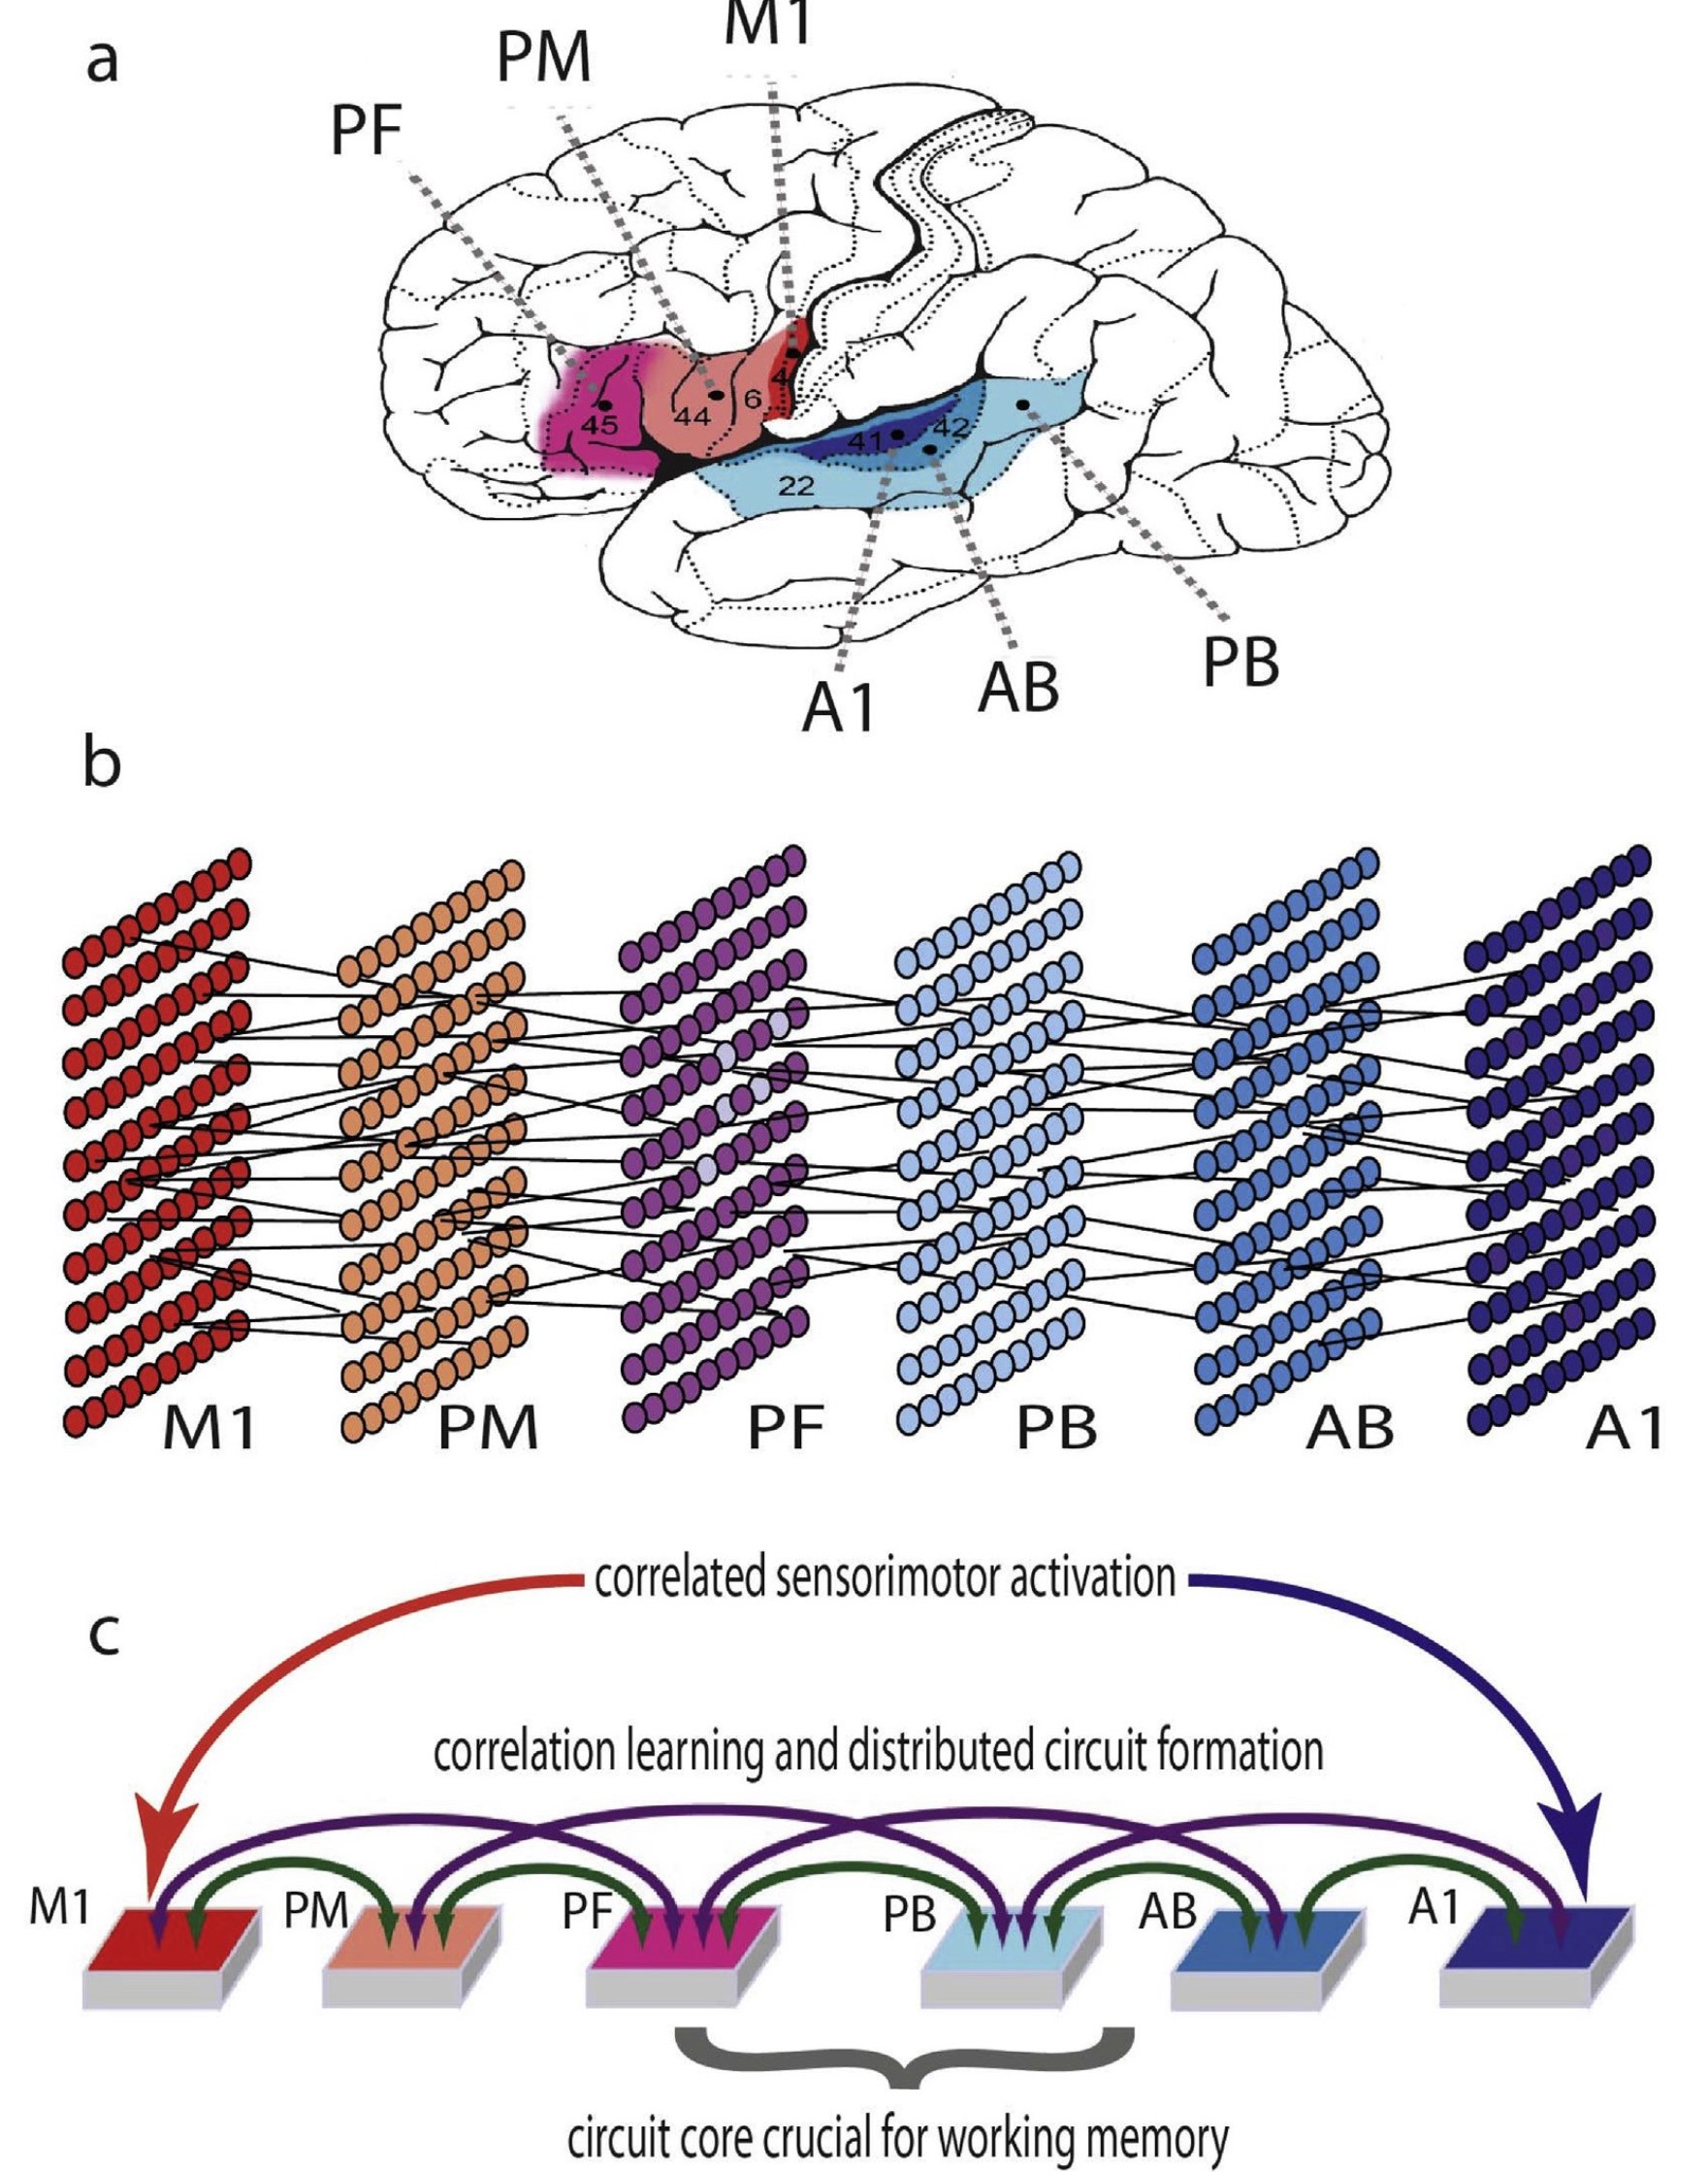
\includegraphics[width=0.8\linewidth]{figures/chap2-fig1} 

}

\caption{Modèle de simulation en 6 couches pour l’apprentissage de mots formant une APC, liant structures motrices et perceptives. Le modèle a implémenté six aires primaires, de même que la connectivité basée sur les connaissances de la connectivité cérébrale et les processus d’apprentissage par corrélation (hebbien) et d’inhibition (anti-hebbien). Ce modèle a été implémenté pour simuler l’apprentissage par corrélation qui opère lorsqu’un mot est prononcé. L’apprentissage se traduisant par la formation de circuits conceptuels distribués dans différentes régions corticales, y compris dans des zones multimodales et spécifiques à la modalité (e.g., cortex moteurs et visuels). \textbf{a} : aires frontotemporales et pérysylviennes implémentées dans le modèle. \textbf{b} : structure schématisée du réseau. M1 : cortex moteur primaire. PM : cortex prémoteur. PF : cortex préfrontal. PB : aire de brodmann 22 ; AB : cortex auditif secondaire. A1 : cortex auditif primaire. Les flèches qui relient les six aires du réseau donnent un exemple de circuit fonctionnel distribué (réseau de neurones) développé au cours de l'apprentissage de patterns d’action-perception. \textbf{c} : structure de la connectivité entre les six aires du modèle. Figure issue de Garagnani \& Pulvermüller (2016).}\label{fig:chap2-fig1}
\end{figure}

Pour \protect\hyperlink{ref-pulvermuller_neural_2018}{Pulvermüller} (\protect\hyperlink{ref-pulvermuller_neural_2018}{2018a}), ces APC constitueraient la base neuronale du langage et contiendraient les représentations conceptuelles (i.e., des mots et des concepts). En effet, les mécanismes supposés par le modèle APC ont été étayés par plusieurs études de simulation qui montrent comment le mécanisme d'apprentissage par corrélation associative pourrait bien être le mécanisme neurobiologique qui soutient l'incarnation des unités linguistiques (e.g., \protect\hyperlink{ref-garagnani_conceptual_2016}{Garagnani \& Pulvermüller, 2016}; \protect\hyperlink{ref-tomasello_brain_2017}{Tomasello et al., 2017}). Comme représenté dans la figure \ref{fig:chap2-fig1}, ces modèles contraints biologiquement ont été utilisés pour imiter l'apprentissage par corrélation associative des relations conceptuelles entre les formes des mots et leurs référents. Les résultats de l'apprentissage se traduisaient par le développement de circuits fortement connectés reliant les informations relatives aux formes des mots et les informations conceptuelles. Sur la base de ces résultats, \protect\hyperlink{ref-pulvermuller_neural_2018}{Pulvermüller} (\protect\hyperlink{ref-pulvermuller_neural_2018}{2018a}) considère que la formation de ces APC offre un mécanisme neurobiologiquement plausible pour rendre compte de la réutilisation de neurones sensorimoteurs pour la représentation conceptuelle, et de l'ancrage de ces concepts dans l'expérience sensorimotrice.

Pour \protect\hyperlink{ref-pulvermuller_case_2018}{Pulvermüller} (\protect\hyperlink{ref-pulvermuller_case_2018}{2018c}), les concepts abstraits peuvent être directement ancrés dans l'expérience sensorimotrice grâce aux APC (cf.~Figure \ref{fig:chap2-fig5}). Si les mécanismes d'apprentissage hebbien jouent un rôle important pour les concepts concrets, les mécanismes d'apprentissage anti-hebbien seraient déterminants pour l'acquisition et la représentation des concepts abstraits (\protect\hyperlink{ref-pulvermuller_case_2018}{Pulvermüller, 2018c, p. 7}). Il l'illustre notamment avec le concept abstrait de \emph{cause} :

\begin{quote}
``Although causal actions and their effects are very variable, it appears that at least subsets of them share features, which can be motivated neurobiologically. If this is so, the perceptual and action-related features shared by different instances of causation may become key to conceptual binding. {[}\ldots{]} Note that correlation learning commands that neural elements processing idiosyncratic or atypical features of causal acts are not bound into the circuit. {[}\ldots{]} In essence, correlated neuronal activity of partially shared key neurons in relevant modality-related and adjacent convergence areas together with activity of the word form circuit in the perisylvian cortex is the driving force of concept formation. This correlation leads to a cell assembly for the concept of causation, which is distributed across the perisylvian cortex and adjacent multimodal areas but also reaches into sensorimotor fields.''
\end{quote}

Ainsi, pour \protect\hyperlink{ref-pulvermuller_case_2018}{Pulvermüller} (\protect\hyperlink{ref-pulvermuller_case_2018}{2018c}) si les concepts abstraits sont rencontrés dans une variété de situations et n'ont pas de référent perceptif unique, cela n'implique pas que ce qui est commun à l'expérience d'un concept abstrait ne puisse pas être appris par les mécanismes d'apprentissage par corrélation associative. Il devrait exister certaines caractéristiques typiques à l'expérience d'un concept, de sorte que les caractéristiques partiellement partagées puissent être réutilisées pour représenter un concept abstrait (\protect\hyperlink{ref-pulvermuller_case_2018}{Pulvermüller, 2018c}). Autrement dit, comme les caractéristiques partiellement partagées seraient fréquemment activées en même temps que les mots qui les désignent, l'apprentissage par corrélation associative peut s'appliquer aux concepts abstraits (cf.~Figure \ref{fig:chap2-fig5}).

Si la proposition d'un ancrage direct dans l'expérience sensorimotrice est étayée par de nombreuses simulations d'apprentissage conceptuelles de concepts concrets (e.g., \protect\hyperlink{ref-garagnani_conceptual_2016}{Garagnani \& Pulvermüller, 2016}; \protect\hyperlink{ref-tomasello_brain_2017}{Tomasello et al., 2017}), et plus récemment de concepts abstraits émotionnels (e.g., \protect\hyperlink{ref-dreyer_abstract_2018}{Dreyer \& Pulvermüller, 2018}; \protect\hyperlink{ref-vigliocco_neural_2014}{Vigliocco et al., 2014}), il importe maintenant de savoir si un ancrage direct dans l'expérience serait possible pour d'autres types de concepts, comme le concept abstrait de temps. Dans les sections suivantes, après avoir présenté les données disponibles sur l'étude du concept de temps, nous verrons comment le modèle des APC fourni une nouvelle interprétation des données. Précisément, nous proposerons que le concept abstrait de temps pourrait être incarné directement dans l'expérience sensorimotrice, par le biais du mouvement.

\begin{figure}[htbp!]

{\centering 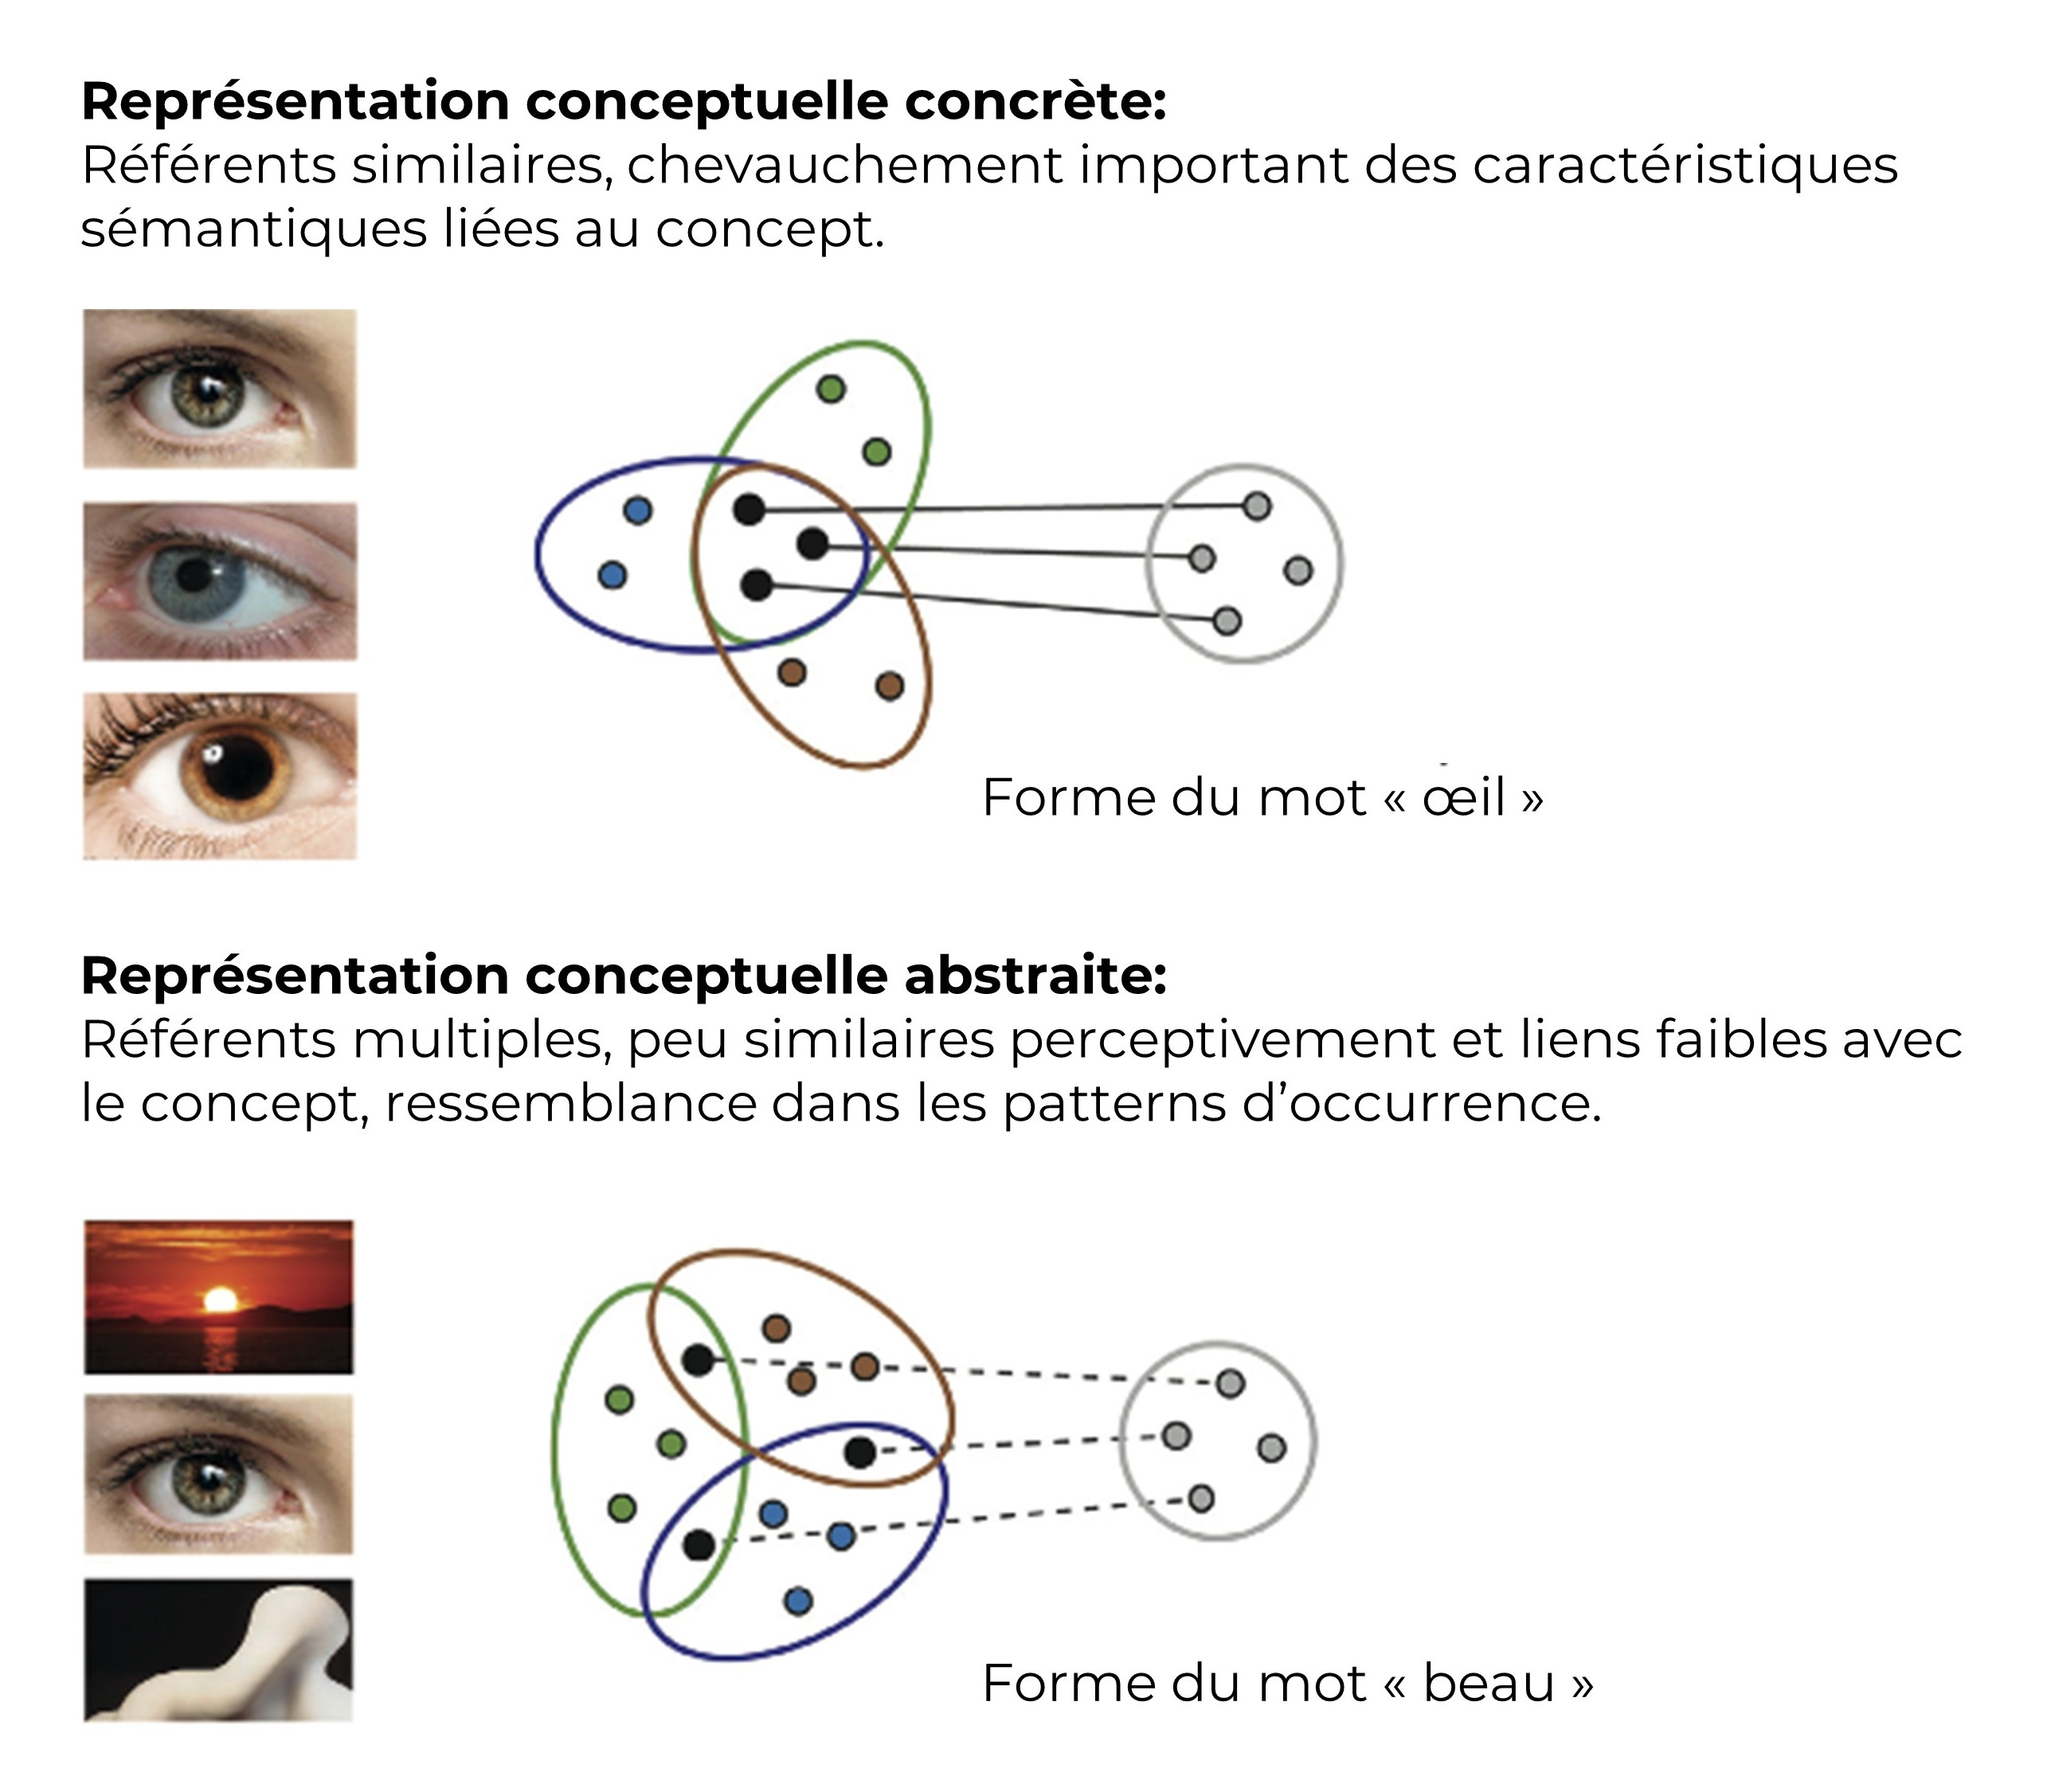
\includegraphics[width=1\linewidth]{figures/chap2-fig5} 

}

\caption{Ancrage par corrélation. Propositions des mécanismes pour l’ancrage des concepts concrets (haut) et abstraits (bas) faites par le modèle des APC (e.g., Pulvermüller, 2018) Si les schémas d’activités sensorimotrices sont peu variables pour les concepts concrets, ils sont en revanche beaucoup plus variables pour les concepts abstraits. Cette différence dans la structure des corrélations qui associent un concept à son référent se traduit par des mécanismes d’ancrage légèrement différents. Dans le cas des concepts concrets, comme la majorité des référents se ressemblent beaucoup, cela conduit rapidement à des représentations prototypiques par l’extraction des caractéristiques communes, fréquemment associées au concept. Les mécanismes hebbien étant essentiels à ce processus. Dans le cadre des concepts abstraits, comme leur référent comprend des situations et des objets très variables, les mécanismes anti-hebbien permettent un ancrage sur les caractéristiques partiellement partagées dans les diverses situations où il est rencontré. Cette faible corrélation entre circuits neuronaux n’implique pas l’absence d’ancrage car les connexions peuvent s’appuyer sur plusieurs patterns sensorimoteurs communs à un concept abstrait. Issue de (Pulvermüller, 2013). Chaque point coloré représente ici une unité activée lors de l’interaction avec un concept, les points gris représentent les unités qui vont être renforcées et intégrées au réseau au cours del'apprentissage.}\label{fig:chap2-fig5}
\end{figure}

\hypertarget{le-temps-comme-cas-duxe9tude-du-traitement-des-concepts-abstraits}{%
\section{Le temps comme cas d'étude du traitement des concepts abstraits}\label{le-temps-comme-cas-duxe9tude-du-traitement-des-concepts-abstraits}}

\epigraph{"The idea of time does not originate in the senses but is presupposed by them… Time is not something objective. It is neither substance nor accident not relation, but a subjective condition, necessary owing to the nature of the human mind, of the coordination of all sensibles [experienced stimuli] according to a fixed law"}{Kant, E. (inaugural dissertation, section 3.14)}

Le temps est un concept particulier, que Fraser désigne comme un étranger familier : s'il est insaisissable et mystérieux, aucune autre partie de notre existence ne pourrait nous paraitre plus intimement familière que le temps (\protect\hyperlink{ref-fraser_time_1988}{Fraser, 1988}). À ce sujet, on cite souvent les propos de Saint Augustin :

\begin{quote}
``What then is time? If no one asks me, I know what it is. If I wish to explain it to him who asks, I do not know.''
\end{quote}

Bien que difficiles à définir, les concepts liés au temps font partie de notre lexique quotidien. En Anglais, parmi les cinq mots les plus utilisés (à savoir : \emph{time}, \emph{person}, \emph{year}, \emph{way} et \emph{day}), trois sur cinq se rapportent au concept de temps (e.g., \protect\hyperlink{ref-buonomano_your_2017}{Buonomano, 2017}; \protect\hyperlink{ref-cooperrider_how_2016}{Cooperrider \& Núñez, 2016}; \protect\hyperlink{ref-kranjec_are_2010}{Kranjec \& Chatterjee, 2010}). Le temps rythme nos conversations et nos vies quotidiennes. Nous parlons du temps qui passe, du temps que prendra telle ou telle activité, de passer du bon temps, de gagner ou encore de perdre du temps.

Le concept de temps est considéré comme abstrait parce qu'il ne possède aucune réalité physique objective (\protect\hyperlink{ref-grondin_physical_2001}{Grondin, 2001}). Pourtant, même si nous ne pouvons pas le voir, le toucher, et encore moins le gouter, nous disposons de la merveilleuse capacité de \emph{percevoir} le temps qui passe et de nous représenter ce qui est passé et ce qui sera. Tout ceci fait du concept de temps le parfait cas d'étude pour appréhender l'acquisition et la représentation des concepts abstraits.

Notons que parler du temps comme un concept unique serait commettre la même erreur que considérer l'ensemble des concepts abstraits comme un tout unitaire (cf.~section \ref{defa}). Parmi les concepts temporels, nous pouvons distinguer ceux qui désignent la durée des évènements dans le temps (e.g., minutes, secondes) de ceux qui désignent l'ordre des événements dans le temps (e.g., le passé et le futur). Et ces deux concepts temporels seraient radicalement différents (\protect\hyperlink{ref-nunez_tangle_2013}{Núñez \& Cooperrider, 2013}). Nous avons précédemment établi (section \ref{incarnation}) que différents sous-types de concepts pouvaient être représentés par différents patterns d'activations corticales, parce qu'ils renvoient à des situations différentes (\protect\hyperlink{ref-desai_multifaceted_2018}{Desai et al., 2018}). Parce qu'étudier différents sous-types de concepts abstraits reviendraient à étudier les différentes situations qui sous-tendent leur ancrage, nous avons choisi de ne porter attention qu'aux concepts d'ordre temporels. À partir de maintenant, lorsque nous parlerons du concept de temps, il s'agira des concepts (ordinaux) de passé et de futur (sauf mention contraire).

Dans les prochaines sections, nous présenterons l'état de l'art concernant l'étude des concepts abstraits temporels. Ceci nous permettra d'introduire les questions théoriques et empiriques jusque-là non résolues, que nous aborderons dans les chapitres expérimentaux de ce manuscrit. La majorité de ces données ont été interprétées en faveur de processus de mise en correspondance métaphorique, supposant un ancrage indirect du temps par l'espace concret. Nous développerons cependant dans la deuxième section de ce chapitre, une nouvelle analyse et interprétation des données disponibles, en proposant un ancrage direct du temps par le mouvement.

\hypertarget{axes}{%
\subsection{Des axes spatiaux pour représenter le concept de temps}\label{axes}}

\epigraph{"Why do we believe that events are to be distinguished as past, present and future? I conceive that the belief arises from distinctions in our own experience"}{McTaggart, J. E. (1908, p.471)}

Comme évoqué dans la section \ref{metaphor}, les théories de la métaphore conceptuelle ont dominé l'étude des mécanismes de l'acquisition des concepts abstraits (e.g., \protect\hyperlink{ref-boroditsky_metaphoric_2000}{Boroditsky, 2000}, \protect\hyperlink{ref-boroditsky_does_2001}{2001}; \protect\hyperlink{ref-lakoff_philosophy_1999}{Lakoff \& Johnson, 1999}). Le concept abstrait le plus étudié à l'appui de ce cadre théorique est le concept de temps (\protect\hyperlink{ref-boroditsky_metaphoric_2000}{Boroditsky, 2000}, \protect\hyperlink{ref-boroditsky_does_2001}{2001}; pour revues voir \protect\hyperlink{ref-bender_mapping_2014}{Bender \& Beller, 2014}; \protect\hyperlink{ref-bonato_when_2012}{Bonato et al., 2012}; \protect\hyperlink{ref-cooperrider_across_2009}{Cooperrider \& Núñez, 2009}). Pour rappel, les théories conceptuelles supposent que la représentation conceptuelle du temps serait de nature spatiale. Ceci serait rendu possible parce que les représentations conceptuelles concrètes (e.g., l'espace), fondées directement dans l'expérience sensorimotrice, seraient recyclées pour soutenir les représentations abstraites (e.g., le temps), leur fournissant un ancrage indirect dans l'expérience sensorimotrice (e.g., \protect\hyperlink{ref-boroditsky_metaphoric_2000}{Boroditsky, 2000}, \protect\hyperlink{ref-boroditsky_does_2001}{2001}; \protect\hyperlink{ref-lakoff_philosophy_1999}{Lakoff \& Johnson, 1999}). La conséquence d'un tel processus se traduirait dans notre façon de conceptualiser le temps (de le « penser ») et, par voie de conséquence, dans notre langage quotidien, par l'utilisation de métaphores spatiales pour parler du temps. Ainsi, la majorité des efforts fournis visaient à mettre en évidence les interactions entre l'espace et le temps en proposant des taxonomies de métaphores inter-domaines (pour revues sur l'axe avant-arrière voir \protect\hyperlink{ref-bender_mapping_2014}{Bender \& Beller, 2014}; \protect\hyperlink{ref-nunez_future_2006}{Núñez \& Sweetser, 2006}). Cette approche a permis de mettre en lumière une relative universalité de l'utilisation de métaphores spatiales pour parler du temps (même si leur utilisation diffère d'une culture à une autre ; e.g., \protect\hyperlink{ref-nunez_tangle_2013}{Núñez \& Cooperrider, 2013}). Intuitivement, le temps semble être une dimension spatiale continue où nous pouvons localiser le passé, le présent et le futur : notre enfance est derrière nous, notre avenir est devant nous, la fin de cette introduction est proche.

Ces deux dernières décennies, les propositions des théories conceptuelles, bien qu'initialement développées en linguistique (e.g., \protect\hyperlink{ref-lakoff_philosophy_1999}{Lakoff \& Johnson, 1999}), ont également été examinées en psychologie et en neurosciences cognitives (\protect\hyperlink{ref-borghi_words_2014}{Borghi \& Binkofski, 2014}). L'hypothèse la plus populaire pour étudier comment l'individu spatialise le temps est la proposition d'une \emph{ligne mentale temporelle} (désormais MTL pour mental timeline). Cette hypothèse propose un système de coordonnées spatiales linéaire pour organiser spatialement le concept de temps (pour revues, voir \protect\hyperlink{ref-bender_mapping_2014}{Bender \& Beller, 2014}; \protect\hyperlink{ref-bonato_when_2012}{Bonato et al., 2012}; \protect\hyperlink{ref-lewandowska-tomaszczyk_mental_2016}{Eikmeier et al., 2016}). Dans ce cadre, le temps serait représenté en termes de positions spatiales où le passé et le futur serait organisé linéairement et de façon relative à un repère spatial donné (généralement le corps de l'individu, e.g., \protect\hyperlink{ref-bonato_when_2012}{Bonato et al., 2012}; \protect\hyperlink{ref-weger_time_2008}{Weger \& Pratt, 2008}).

Deux axes spatiaux ont été rapportés : un premier axe vertical avec le passé localisé derrière et le futur devant l'individu (pour revue voir \protect\hyperlink{ref-bender_mapping_2014}{Bender \& Beller, 2014}), et un second axe horizontal organisé de gauche à droite avec le passé localisé à gauche du corps et le futur à droite du corps (notez que la direction de ces deux axes peut varier en fonction de la culture). Dans ce cadre, il est proposé que le traitement d'un concept temporel (e.g., passé ou futur) serait sous-tendu par l'activation de sa coordonnée spatiale, formant ainsi une MTL (e.g., \protect\hyperlink{ref-santiago_time_2007}{Santiago et al., 2007}; \protect\hyperlink{ref-sell_processing_2011}{Sell \& Kaschak, 2011}). Cette influence du traitement spatial sur le traitement de concepts temporels est aujourd'hui bien établie, comme en témoigne l'ensemble d'études faisant état d'effets de congruence dite spatio-temporelle, entre le contenu temporel de mots ou de phrases à traiter et les coordonnées spatiales associées aux stimuli (pour revues, voir \protect\hyperlink{ref-bonato_when_2012}{Bonato et al., 2012}; \protect\hyperlink{ref-lewandowska-tomaszczyk_mental_2016}{Eikmeier et al., 2016}).

Dans le domaine du langage, l'une des premières études à avoir mis en évidence un tel effet de congruence spatio-temporelle pour le traitement de concepts temporels est celle de \protect\hyperlink{ref-santiago_time_2007}{Santiago et al.} (\protect\hyperlink{ref-santiago_time_2007}{2007}). Dans cette étude, les participant·e·s devaient déterminer si des mots présentés à droite ou à gauche d'une croix de fixation appartenaient au passé ou au futur (tâche de catégorisation temporelle). En plus de la position des stimuli sur l'écran, l'espace de réponse sur le clavier a aussi été manipulé, avec des réponses localisées à gauche du clavier (avec main gauche) et réponses à droite du clavier (avec main droite). Par exemple, un mot au passé pouvait être associé soit à une réponse donnée avec la main gauche et une touche sur la partie gauche du clavier (condition congruente) soit à une réponse donnée avec la main droite et une touche sur la partie droite du clavier (condition incongruente). Les résultats de cette étude montrent que le traitement des mots au passé est plus rapide lorsqu'ils sont présentés dans l'espace gauche de l'écran, mais aussi lorsque les participant·e·s répondent avec leur main gauche, alors que le traitement des mots au futur est plus rapide lorsqu'ils sont présentés dans l'espace droit de l'écran et lorsque la réponse sur le clavier est à droite (voir aussi, \protect\hyperlink{ref-torralbo_flexible_2006}{Torralbo et al., 2006}). Ces résultats montrent que la représentation du temps serait associer à des informations spatiales horizontales gauche-droite (i.e., la MTL) de manière relative à l'espace périperisonnel de chaque individu.

Dans une autre étude, demander à des participant·e·s de garder en mémoire de travail des stimuli liés aux concepts de passé ou de futur s'est traduit par des effets facilitateurs pour la détection de stimuli présentés soit à gauche soit à droite de l'écran (\protect\hyperlink{ref-ouellet_thinking_2010}{Ouellet, Santiago, Funes, et al., 2010}; voir aussi \protect\hyperlink{ref-weger_time_2008}{Weger \& Pratt, 2008}). Ces résultats suggèrent que la temporalité (passé ou futur) des stimuli pouvait induire des changements (shifts) attentionnels dans l'espace correspondant à l'organisation supposée de la MTL (\protect\hyperlink{ref-ouellet_thinking_2010}{Ouellet, Santiago, Funes, et al., 2010}; voir aussi \protect\hyperlink{ref-weger_time_2008}{Weger \& Pratt, 2008}). Le même effet de congruence spatio-temporelle pour la catégorisation de mots au passé ou au futur avec réponses bi-manuelles au clavier a été rapporté quand les stimuli étaient présentés en modalité auditive (\protect\hyperlink{ref-kong_space-time_2012}{Kong \& You, 2012}), mais aussi pour le traitement de phrases entières (\protect\hyperlink{ref-eikmeier_how_2015}{Eikmeier, Alex-Ruf, et al., 2015}; \protect\hyperlink{ref-maienborn_we_2015}{Maienborn et al., 2015}; \protect\hyperlink{ref-ulrich_leftright_2010}{Ulrich \& Maienborn, 2010}). Enfin, des données issues de patients présentant une négligence spatiale unilatérale (consécutive à une lésion pariétale droite), dont le tableau clinique se caractérise principalement par une négligence attentionnelle de l'hémichamp gauche, montrent également des difficultés pour catégoriser des évènements comme appartenant au passés (par rapport à des évènements futurs) ou se représenter des évènements passés (e.g., \protect\hyperlink{ref-anelli_effects_2018}{Anelli et al., 2018}; \protect\hyperlink{ref-saj_patients_2014}{Saj et al., 2014}).

Pour résumer, ces effets de congruence spatio-temporelle semblent émerger lorsqu'une tâche temporelle implique différentes coordonnées spatiales, indépendamment du fait que la manipulation spatiale soit déterminée par la latéralisation des réponses manuelles, ou par la latéralisation spatiale de la cible temporelle à traiter, visuellement ou auditivement (e.g., \protect\hyperlink{ref-kong_space-time_2012}{Kong \& You, 2012}; \protect\hyperlink{ref-santiago_time_2007}{Santiago et al., 2007}). Selon le principe établi par \protect\hyperlink{ref-sternberg_discovery_1969}{Sternberg} (\protect\hyperlink{ref-sternberg_discovery_1969}{1969}) section \ref{challenge}, ces effets de congruence spatio-temporelle suggèrent l'utilisation de structures corticales communes pour le traitement de l'espace et du temps. De plus, ces données suggèrent une utilisation automatique de structures corticales spatiales pour le traitement lexical du concept de temps (e.g., \protect\hyperlink{ref-santiago_time_2007}{Santiago et al., 2007}; \protect\hyperlink{ref-sell_processing_2011}{Sell \& Kaschak, 2011}). Pour les tenants des théories conceptuelles, ces observations ont été interprétées en faveur d'une mise en correspondance métaphorique inter-domaines (\protect\hyperlink{ref-casasanto_time_2008}{Casasanto \& Boroditsky, 2008}): le temps pourrait bien être indirectement ancré à partir de l'expérience de l'espace concret.

Cependant, comme nous l'avons détaillé précédemment, certains auteurs ont questionné la notion d'expérience concrète de l'espace (e.g., \protect\hyperlink{ref-kranjec_are_2010}{Kranjec \& Chatterjee, 2010}). En outre, observer des effets de congruence spatio-temporelle n'est pas suffisant pour conclure que c'est parce que le concept d'espace est recyclé pour le concept de temps (ancrage indirect) que l'on observe de tels chevauchement entre espace et temps. Selon les discussions évoquées précédemment (cf.~section \ref{incarnation}, ou encart \ref{meta}), il est possible que les chevauchements rapportés pour le traitement spatial et le traitement temporel puisse être expliqués par le partage de caractéristiques fonctionnelles communes en situation (e.g., \protect\hyperlink{ref-anderson_after_2014}{Anderson, 2014}; \protect\hyperlink{ref-kranjec_are_2010}{Kranjec \& Chatterjee, 2010}).

La méta-analyse de \protect\hyperlink{ref-von_sobbe_space-time_2019}{von Sobbe et al.} (\protect\hyperlink{ref-von_sobbe_space-time_2019}{2019}) met en évidence que si l'effet de congruence spatio-temporelle parait robuste, il ne l'est en réalité que lorsque la tâche à réaliser par les participant·e·s implique un traitement explicite du contenu temporel des stimuli (e.g., lors d'une tâche de catégorisation temporelle). L'effet se trouve largement diminué, voire absent, lorsque la tâche des participant·e·s n'implique pas de traitement explicite du temps (\protect\hyperlink{ref-maienborn_we_2015}{Maienborn et al., 2015}; \protect\hyperlink{ref-ulrich_leftright_2010}{Ulrich \& Maienborn, 2010}, exp. 2 et 3 pour l'axe gauche-droit). Selon \protect\hyperlink{ref-von_sobbe_space-time_2019}{von Sobbe et al.} (\protect\hyperlink{ref-von_sobbe_space-time_2019}{2019}), comme l'effet de congruence spatio-temporelle est absent lors de tâches où le contenu temporel des stimuli n'a aucune pertinence pour la réussite de la tâche (appelée tâche \emph{temporelle} \emph{implicite}, \protect\hyperlink{ref-von_sobbe_space-time_2019}{von Sobbe et al., 2019}), alors on ne peut pas conclure que ce système de coordonnées spatiales (la MTL) est automatiquement impliqué dans le traitement du concept de temps (hypothèse soutenue par les théories incarnées, cf.~section \ref{pred}). L'effet de congruence spatio-temporelle pourrait, de manière plus parcimonieuse, être expliqué par un accès facilité en mémoire. En effet, il se pourrait qu'une association gauche-passé et droite-future stockée en mémoire soit réutilisée pendant une tâche temporelle \emph{explicite.}

Une seule étude rapportée dans la méta-analyse de \protect\hyperlink{ref-von_sobbe_space-time_2019}{von Sobbe et al.} (\protect\hyperlink{ref-von_sobbe_space-time_2019}{2019}) montre un effet de congruence spatio-temporelle pour une tâche \emph{temporelle} \emph{implicite} ; celle de \protect\hyperlink{ref-sell_processing_2011}{Sell \& Kaschak} (\protect\hyperlink{ref-sell_processing_2011}{2011}) répliquée récemment par \protect\hyperlink{ref-scheifele_replication_2018}{Scheifele et al.} (\protect\hyperlink{ref-scheifele_replication_2018}{2018}), portant sur l'axe vertical avant-arrière. Dans cette étude, les participant·e·s devaient juger si des phrases (faisant référence à des évènements passés ou futurs) étaient grammaticalement correctes ou non. Les participant·e·s donnaient leur réponse sous deux conditions : i) soit en réalisant un mouvement dirigé dans l'espace avant-arrière (e. g., actionner un joystick vers l'avant pour répondre oui), ii) soit en exécutant des réponses statiques sur un clavier avec les mains disposées verticalement, l'une avant l'autre sur l'axe vertical. Les résultats rapportés par \protect\hyperlink{ref-sell_processing_2011}{Sell \& Kaschak} (\protect\hyperlink{ref-sell_processing_2011}{2011}) montrent un effet de congruence spatio-temporelle uniquement lorsque la réponse des participant·e·s nécessitait un mouvement dans l'espace, et non pour les réponses motrices statiques (actionner la touche). Notons que cette différence de résultats observée entre la condition mouvement dirigé et mouvement statique n'a pas été discutée par \protect\hyperlink{ref-von_sobbe_space-time_2019}{von Sobbe et al.} (\protect\hyperlink{ref-von_sobbe_space-time_2019}{2019}). Selon \protect\hyperlink{ref-von_sobbe_space-time_2019}{von Sobbe et al.} (\protect\hyperlink{ref-von_sobbe_space-time_2019}{2019}) l'émergence d'un effet de congruence spatio-temporelle pour une tâche temporelle \emph{implicite} dans les résultats de \protect\hyperlink{ref-sell_processing_2011}{Sell \& Kaschak} (\protect\hyperlink{ref-sell_processing_2011}{2011}) ne serait pas la preuve d'une activation automatique d'une MTL (voir aussi \protect\hyperlink{ref-maienborn_we_2015}{Maienborn et al., 2015}; \protect\hyperlink{ref-ulrich_past_2012}{Ulrich et al., 2012}; \protect\hyperlink{ref-von_sobbe_space-time_2019}{von Sobbe et al., 2019, p. 15}), mais pourrait être expliquée par la complexité de la tâche demandée aux participant·e·s :

\begin{quote}
``Hence, whether or not the mental timeline is activated automatically seems to depend on whether or not the temporal order information can be processed without using the mental timeline as part of the build-up of a situation model (Scheifele et al., 2018). Only when discourses with larger time shifts are processed, temporal complexity might ``get the upper hand'' (Scheifele et al., 2018, p.~10), thus eliciting the build-up of a mental situation model to manage the temporal order information: While single sentences usually only refer to one event, multi-sentences discourses with large time shifts refer to several clearly distinguishable and separate events that necessitate a sequencing by means of a localization on the mental timeline.''
\end{quote}

Cependant, il semble que la question de la différence entre mouvement dynamique (i.e., spatialement dirigé) et statique pourrait être une piste intéressante à creuser. Comme évoqué dans les sections \ref{pred} et \ref{incarnation}, si la représentation du concept de temps est ancrée dans des réseaux distribués alors le traitement de ce concept (qu'il soit explicitement ou implicitement exigé par la tâche), devrait se traduire par une activation automatique de l'ensemble du circuit auquel il appartient (\protect\hyperlink{ref-kranjec_are_2010}{Kranjec \& Chatterjee, 2010}; \protect\hyperlink{ref-pulvermuller_case_2018}{Pulvermüller, 2018c}). Dans ce cadre, l'hypothèse d'un effet de facilitation d'accès en mémoire (e.g., \protect\hyperlink{ref-von_sobbe_space-time_2019}{von Sobbe et al., 2019}) n'est pas compatible avec la prédiction d'une activation automatique.

Comme ces études se concentrent sur l'association entre l'espace et le temps, les manipulations expérimentales se focalisent principalement sur l'influence de la localisation spatiale d'un stimulus temporel sur son traitement (ou de la localisation de la réponse). De plus, comme discuté dans la section \ref{lim-con}, il est possible que le concept de temps puisse être incarné directement dans l'expérience temporelle même, de façon plus ou moins indépendante avec l'espace (e.g., \protect\hyperlink{ref-flusberg_connectionist_2010}{Flusberg et al., 2010}; \protect\hyperlink{ref-kranjec_are_2010}{Kranjec \& Chatterjee, 2010}).

Dans les études où le traitement des concepts abstraits temporels ne porte pas explicitement sur le contenu temporel des stimuli (e.g., \protect\hyperlink{ref-aguirre_potential_2017}{Aguirre \& Santiago, 2017}; \protect\hyperlink{ref-ulrich_leftright_2010}{Ulrich \& Maienborn, 2010}), il est envisageable que la manipulation expérimentale pour étudier le traitement du concept de temps ne permette pas d'appréhender assez finement les structures cérébrales spécifiquement en charge du traitement conceptuel. Par exemple, il est possible que le contexte d'occurrence du concept de temps ne soit pas directement manipulé. Comme l'explication d'un ancrage indirect du concept de temps proposée par les théories conceptuelles est limitée (cf.~section \ref{lim-con}), il importe d'étudier quelles pourraient être les situations répétées dans lequel le concept de temps pourrait être ancré directement (e.g., \protect\hyperlink{ref-barsalou_moving_2018}{Barsalou et al., 2018}; \protect\hyperlink{ref-kranjec_are_2010}{Kranjec \& Chatterjee, 2010}; \protect\hyperlink{ref-pulvermuller_neural_2018}{Pulvermüller, 2018a}, \protect\hyperlink{ref-pulvermuller_case_2018}{2018c}).

L'hypothèse que nous avons formulée porte sur le rôle du mouvement.\footnote{À savoir : exécuter un mouvement dirigé dans l'espace ou exécuter une réponse motrice statique en appuyant sur une touche.} En effet, nous proposons que la manipulation de l'amplitude et de la direction du mouvement puisse expliquer la différence de résultats observés entre tâches temporelles implicites et explicites rapportées dans la méta-analyse de \protect\hyperlink{ref-von_sobbe_space-time_2019}{von Sobbe et al.} (\protect\hyperlink{ref-von_sobbe_space-time_2019}{2019}). Dans la section suivante, nous examinerons les arguments empiriques à l'appui de l'hypothèse d'un rôle clé du mouvement pour la représentation des concepts abstraits temporels. Notamment, nous verrons comment le mouvement pourrait expliquer les chevauchements observés entre espace et temps, et comment certains types de mouvements répétés dans l'espace pourraient être un bon candidat pour l'ancrage direct des concepts abstraits temporels dans l'expérience. De telles observations appuieraient les propositions faites par le modèle des APC (e.g., \protect\hyperlink{ref-pulvermuller_neural_2018}{Pulvermüller, 2018a}, \protect\hyperlink{ref-pulvermuller_case_2018}{2018c}), à savoir qu'un ancrage \emph{direct} dans l'expérience sensorimotrice d'un concept abstrait est possible (cf.~section \ref{pred}), et que le traitement de ce concept devrait activer automatiquement le réseau distribué auquel il appartient (cf.~section \ref{pred}).

\hypertarget{ancrage}{%
\subsection{Ancrage direct des concepts abstraits temporels dans l'expérience sensorimotrice : l'hypothèse du mouvement}\label{ancrage}}

Le rôle du mouvement pour la représentation du temps n'est pas une hypothèse nouvelle. Les théories conceptuelles abordent également la notion de mouvement (e.g., \protect\hyperlink{ref-boroditsky_roles_2002}{Boroditsky \& Ramscar, 2002}). Par exemple, \protect\hyperlink{ref-boroditsky_roles_2002}{Boroditsky \& Ramscar} (\protect\hyperlink{ref-boroditsky_roles_2002}{2002}) ont montré que demander à des participant·e·s d'imaginer que le temps se déplace vers eux ou, alternativement, que ce sont eux qui avancent dans le temps, était suffisant pour induire un changement de perspective sur les évènements passés et futurs. Ces résultats impliquent que la MTL comprendrait non seulement des informations de localisation dans l'espace, mais aussi des informations liées au mouvement. De même, l'utilisation de l'espace pour représenter le temps se retrouve aussi dans les gestes qui accompagnent la parole. Des observations rapportent que la parole est accompagnée de mouvements manuels dirigés vers la gauche lorsque les locuteurs parlent d'évènements passés, et vers la droite pour parler d'évènements futurs (e.g., \protect\hyperlink{ref-casasanto_hands_2012}{Casasanto \& Jasmin, 2012}; \protect\hyperlink{ref-nunez_future_2006}{Núñez \& Sweetser, 2006}). Enfin, s'il existe des métaphores spatiales sur l'axe postéro-antérieur (i.e., avant-arrière), notons qu'il ne semble pas exister de métaphores spatiales pour représenter les évènements passés et futurs sur un axe gauche-droit (Casasanto \& Jasmin, 2012), ce qui semble contredire la prédiction des théories conceptuelles (cf.~section \ref{incarnation}), selon laquelle la mise en correspondance métaphorique serait observable dans le langage (e.g., \protect\hyperlink{ref-lakoff_philosophy_1999}{Lakoff \& Johnson, 1999}). Enfin, notons que dans ce cadre, la part attribuée au mouvement dans ces effets de congruence spatio-temporelle est de second ordre. En effet, les théories conceptuelles considèrent que si le mouvement spatial réalisé par le sujet est cohérent avec l'organisation spatiale du temps, ce serait une conséquence du recyclage de l'expérience de l'espace concret pour le temps.

L'hypothèse alternative consiste à considérer, sur la base du principe de réutilisation neuronale (sections \ref{principe-reuse}, et \ref{lim-con}), que si deux domaines ont des correspondances fonctionnelles communes dans l'expérience (e.g., planification et locomotion motrice, \protect\hyperlink{ref-anderson_after_2014}{Anderson, 2014}) alors ils devraient utiliser des structures neuronales communes, ce qui expliquerait les chevauchements corticaux et la possible observation de relation métaphorique entre les deux domaines (comme une conséquence ; cf.~encart \ref{meta}). Nous proposons que si temps et espace sont intimement liés, c'est parce qu'ils sont vécus ensemble lors de la planification et de l'exécution du mouvement. Nous expérimentons quotidiennement des expériences perceptives de mouvements qui pourraient être le fondement clé de l'ancrage du concept de temps et des chevauchements corticaux entre temps et espace (He et al., 2021).

À ce sujet, une autre hypothèse populaire pour rendre compte de la relation étroite entre temps et espace est la théorie des ordres de grandeurs (désormais ATOM pour a theory of magnitude), qui postule un rôle essentiel de mouvement pour la cognition spatiale, temporelle et numérique (e.g., \protect\hyperlink{ref-bueti_parietal_2009}{Bueti \& Walsh, 2009}; \protect\hyperlink{ref-walsh_theory_2003}{Walsh, 2003}). Précisément, la théorie ATOM propose que la transformation sensorimotrice pour l'action soit le mécanisme de base qui sous-tend la cognition temporelle et la cognition spatiale. Dans ce cadre, il n'est pas proposé que le temps serait de nature spatiale, mais qu'il existe un système commun pour le traitement des ordres de grandeurs (espace, temps, et nombre), qui se développerait grâce au mouvement. Ainsi, il est proposé que les chevauchements corticaux qui existent pour le temps et l'espace résultent de leur traitement parallèle pour la réalisation du mouvement (\protect\hyperlink{ref-bueti_parietal_2009}{Bueti \& Walsh, 2009}; \protect\hyperlink{ref-walsh_theory_2003}{Walsh, 2003}). En effet, comme chaque mouvement réalisé est le produit d'un couplage parallèle et continu de coordonnées spatiales et temporelles, l'individu apprendrait les associations espace-temps lors de la planification et de l'exécution d'actions. Cette utilisation commune expliquerait l'émergence d'un système commun pour le traitement du temps et de l'espace sur lequel serait venu se greffer, plus tard (phylogénétiquement parlant), le traitement des nombres (\protect\hyperlink{ref-bueti_parietal_2009}{Bueti \& Walsh, 2009}; \protect\hyperlink{ref-walsh_theory_2003}{Walsh, 2003}). Ainsi, étant donné que l'espace et le temps partagent des réseaux communs, la théorie ATOM postule que nous devrions observer des interactions spatio-temporelles, et que le traitement du temps devrait interférer avec les réponses sensorimotrices proximales(i.e., des effecteurs comme les mains, \protect\hyperlink{ref-bueti_parietal_2009}{Bueti \& Walsh, 2009}) .

Si la théorie ATOM a été initialement formulée pour rendre compte des données qui s'intéressent au concept de durée temporelle, elle semble tout aussi pertinente pour la conceptualisation de l'ordre temporel. En effet, notons que pour réaliser un mouvement, les coordonnées temporelles qui vont être traitées correspondent non seulement à la durée du mouvement, mais aussi à la séquence, l'ordre de ce mouvement, avec un avant et un après. Pour le dire autrement, si le mouvement est aussi important pour le traitement de l'ordre des évènements dans le temps que pour le traitement de la durée, alors il est possible que la représentation du temps soit sous-tendue par des structures corticales motrices.

En somme, il semble que le mouvement soit un candidat pertinent pour proposer un cadre d'ancrage direct dans l'expérience sensorimotrice des concepts abstraits temporels. Notamment, le mécanisme proposé par la théorie ATOM pour expliquer comment le mouvement provoquerait des chevauchements corticaux entre différents ordres de grandeur est cohérent avec le principe de réutilisation neuronale et les mécanismes d'apprentissage par corrélation associative (e.g., \protect\hyperlink{ref-anderson_after_2014}{Anderson, 2014}; \protect\hyperlink{ref-pulvermuller_case_2018}{Pulvermüller, 2018c}).

\hypertarget{ancrage-direct-des-concepts-abstraits-temporels-par-les-mouvements-duxe9criture-et-de-lecture}{%
\subsection{Ancrage direct des concepts abstraits temporels par les mouvements d'écriture et de lecture}\label{ancrage-direct-des-concepts-abstraits-temporels-par-les-mouvements-duxe9criture-et-de-lecture}}

À ce stade, il importe de se demander pourquoi les concepts d'ordre temporels (passé et futur) se retrouvent organisés spatialement en une MTL gauche-droite (ou avant-arrière) ? L'hypothèse des APC est qu'un concept serait ancré dans des réseaux distribués activés lors d'interactions répétées avec ce concept grâce aux mécanismes d'apprentissage par corrélation hebbien et anti-hebbien (\protect\hyperlink{ref-pulvermuller_case_2018}{Pulvermüller, 2018c}). Si le mouvement est en effet l'expérience sensorimotrice qui sous-tend l'ancrage direct du concept de temps, quels mouvements (caractérisables par des coordonnées spatiales gauche-droite ou avant-arrière) pourraient être suffisamment répétés et dans lequel le passé et le futur seraient expérimentés, pourraient sous-tendre l'ancrage des concepts de passé et de futur ?

Pour répondre à cette question, les données interculturelles existantes, qui se sont intéressées à l'effet de congruence spatio-temporelle sur l'axe horizontale gauche-droit, fournissent des pistes intéressantes. En effet, si jusqu'ici nous avons mentionné des effets de congruence spatio-temporelle où les stimuli faisant référence au passé sont traités plus rapidement lorsqu'ils sont associés à l'espace gauche et inversement pour le futur (e.g., \protect\hyperlink{ref-kong_space-time_2012}{Kong \& You, 2012}; \protect\hyperlink{ref-santiago_time_2007}{Santiago et al., 2007}; \protect\hyperlink{ref-torralbo_flexible_2006}{Torralbo et al., 2006}), notons que cette association gauche-passé et droite-future n'est valable que pour les individus pour lesquels le geste d'écriture et le mouvement des yeux pendant la lecture vont de la gauche vers la droite.

Par exemple, \protect\hyperlink{ref-fuhrman_cross-cultural_2010}{Fuhrman \& Boroditsky} (\protect\hyperlink{ref-fuhrman_cross-cultural_2010}{2010}) ont montré des représentations spatio-temporelles différentes en fonction du système d'écritures des participant·e·s: alors que les locuteurs anglophones (qui écrivent et lisent de la gauche vers la droite) organisent le passé et le futur de la gauche vers la droite, les locuteurs hébreux (qui écrivent et lisent de la droite vers la gauche) montrent le patron de résultats inverse. Des résultats intéressants ont aussi été observés chez des participant·e·s mandarins où le système d'écriture et de lecture suit un axe vertical, avec le passé associé au haut et le futur au bas (\protect\hyperlink{ref-boroditsky_english_2011}{Boroditsky et al., 2011}). Dernier exemple important, \protect\hyperlink{ref-pitt_reading_2016}{Pitt \& Casasanto} (\protect\hyperlink{ref-pitt_reading_2016}{2016}) ont montré qu'un entrainement préalable de quelques minutes pendant lequel les participant·e·s devaient lire en miroir (i.e., dans le sens opposé de leur système d'écriture) suffisait à inverser l'effet de congruence spatio-temporelle.

Notons que pour la MTL postéro-antérieure (i.e., avant-arrière), l'hypothèse fournie se centre également sur le rôle du déplacement des invividus (locomotion) dans l'espace (\protect\hyperlink{ref-lewandowska-tomaszczyk_mental_2016}{Eikmeier et al., 2016}, pour revue). Enfin, les données interculturelles auprès de populations sans système d'écriture et de lecture (e.g., les Yupno, un groupe aborigène de Papouasie-Nouvelle-Guinée) semblent également montrer l'existence d'une organisation spatiale du temps qui dépend de mouvements allocentriques (i.e., dont le cadre de référence spatiale ne dépend pas du corps de l'individu, e.g., \protect\hyperlink{ref-boroditsky_remembrances_2010}{Boroditsky \& Gaby, 2010}; \protect\hyperlink{ref-nunez_contours_2012}{Núñez et al., 2012}). L'ensemble de ces données seront présentées et discutées plus en profondeur, et en lien avec nos résultats, dans la discussion générale.

L'ensemble de ces observations suggère un rôle central du mouvement pour l'ancrage du concept de temps, et particulièrement ici dans les mouvements répétés réalisés au cours de l'écriture et de la lecture. Si nous reprenons l'exemple donné en introduction du chapitre \ref{chap1}, les mouvements balistiques linéaires que vous êtes en train de réaliser pour lire ces lignes pourraient bien être ceux qui, entre autres, soutiennent votre capacité à conceptualiser des concepts aussi abstraits que le passé ou le futur. Au fur et à mesure que vos yeux se déplacent sur ces lignes, les mots à gauche de chaque fixation représente ce que vous venez de lire (le passé) et les mots à droite ce que vous allez lire (le futur). Si l'influence de la direction du système d'écriture et de lecture pour l'organisation spatiale du temps en une MTL semble établie, le rôle du mouvement per se manque d'étayage empirique.

Pour résumer, les données actuelles suggèrent une réutilisation d'informations spatiales pour représenter le temps. À la lumière des discussions évoquées jusqu'ici, nous proposons une nouvelle analyse et interprétation de ces observations que celle proposée par les théories conceptuelles (i.e., un ancrage indirect). Conformément à l'hypothèse de réutilisation neuronale (\protect\hyperlink{ref-anderson_after_2014}{Anderson, 2014}) et des mécanismes d'apprentissage par corrélation associative (\protect\hyperlink{ref-pulvermuller_neural_2018}{Pulvermüller, 2018a}, e.g., \protect\hyperlink{ref-pulvermuller_case_2018}{2018c}), temps et espace pourraient être étroitement liés parce qu'ils le sont dans le monde physique, par le mouvement. Chaque mouvement que nous exécutons ou que nous observons ne peut se défaire de ses caractéristiques spatiales (i.e., déplacement d'un point dans l'espace à un autre) et temporelles (i.e., un ordre temporel que nous décomposé en un début, un pendant, un avant, un après, puis, une fin). Ainsi, nous pouvons faire l'hypothèse que c'est parce que nous répétons des mouvements d'écriture et de lecture qui débutent dans une coordonnée de l'espace (e.g., gauche) et se dirigent dans une autre coordonnée de l'espace (e.g., droite), que nous observons des effets de congruence spatio-temporelle qui coïncident avec la direction de notre système d'écriture et de lecture.

Dans la section suivante, nous présenterons un résumé des discussions théoriques et empiriques établies dans ces deux chapitres d'introduction théorique, ainsi que les questions et hypothèses générales qui seront abordées dans les chapitres expérimentaux.

\hypertarget{predictionth}{%
\subsection{Résumé, questions de recherche, et hypothèses}\label{predictionth}}

\epigraph{"The biggest difference between time and space is that you can’t reuse time"}{Furst, E., cité par Wuppuluri, S. (2016, p.9)}

Le premier chapitre nous a permis de présenter et de discuter les enjeux théoriques et épistémologiques que les théories du langage rencontrent aujourd'hui. Notamment, nous avons établi que le défi pour toute théorie qui souhaite étudier le traitement conceptuel est de pouvoir rendre compte des mécanismes d'acquisition et de compréhension des concepts abstraits. En ce sens, nous avons proposé que les théories incarnées fournissent un cadre puissant pour expliquer comment des concepts dénués de caractéristiques physiques (perceptives et tangibles) pouvaient s'ancrer dans un ensemble d'expériences sensorimotrices.

Dans le chapitre \ref{chap2}, nous avons d'abord présenté et discuté les mécanismes proposés par différentes théories incarnées pour rendre compte de l'incarnation des concepts abstraits. Notamment, nous avons proposé que le principe d'un ancrage indirect des concepts abstraits par la mise en correspondance métaphorique se heurtait à plusieurs limites (section \ref{lim-con}), et que les données disponibles pouvaient être mieux expliquées par des mécanismes de réutilisation neuronale. Ainsi, nous avons adopté le postulat d'Anderson, à savoir que s'il existe des métaphores inter-domaines, elles pourraient être la conséquence de l'ancrage et non la cause. L'objectif étant d'apporter des arguments supplémentaires en faveur de processus incarnés pour la représentation conceptuelle abstraite, nous avons considéré que le modèle des circuits d'action-perception (qui repose sur un principe de réutilisation neuronale), semblait être actuellement un bon candidat pour rendre compte des données présentes dans la littérature. Ce modèle théorique propose un ancrage direct dans l'expérience sensorimotrice pour les concepts abstraits et prédit une activation automatique de l'ensemble du circuit auquel il appartient lors de son traitement (qu'il soit explicite ou implicite). Enfin, au vu de la grande diversité des concepts abstraits, nous avons choisi de n'étudier qu'un seul sous-type de concept abstrait : les concepts d'ordre temporel de passé et futur.

Après avoir présenté un aperçu des données existantes sur l'étude des concepts abstraits temporels, nous avons proposé que le concept de temps pourrait être ancré directement dans l'expérience sensorimotrice du mouvement. Cette hypothèse pourrait notamment expliquer les données existantes faisant états d'effets de congruence spatio-temporelle et les inconsistances de résultats observées entre tâches temporelles explicite et implicite (cf.~section \ref{axes}). Enfin, si l'ancrage des concepts abstraits temporels dans le mouvement passe effectivement par des mécanismes d'apprentissage par corrélation hebbienne et anti-hebbienne, il importe de se demander quels mouvements spatiaux peuvent être suffisamment répétés au cours de l'ontogénie pour former in fine une représentation conceptuelle des concepts de passé et de futur. Dans ce cadre, les données présentées suggèrent que les mouvements réalisés pour lire ou pour écrire sont des candidats pertinents, comme en témoignent les données interculturelles discutées dans la section \ref{ancrage}.

\newpage

\begin{vplace}[1]

\begin{summary}{Résumé du Chapitre\getcurrentref{chapter}}{\chaptercolor}

À la lumière des discussions engagées dans ces deux chapitres théoriques, les travaux que nous avons menés avaient plusieurs objectifs. Premièrement, il s'agissait d’apporter des arguments empiriques en faveur d’un ancrage direct du concept abstrait de temps dans l’expérience sensorimotrice. Deuxièmement, cela permettait de tester plus directement le rôle du mouvement pour la représentation spatiale gauche-droite du temps. Troisièmement, de manière indirecte, il s'agissait de tester la prédiction faite par le modèle des APC, à savoir celle d’une activation automatique des structures corticales réutilisées pour le traitement du concept de temps. Ceci a été fait en utilisant des tâches de décision lexicale où l’attention des participant·e·s ne portait pas explicitement sur le contenu temporel des stimuli. De telles observations permettraient notamment d’apporter des éléments de réponse à la controverse concernant l’hypothèse d’une activation automatique de structures corticales motrices et spatiales pour la représentation du temps (e.g., von Sobbe et al., 2018).\\

La partie empirique de ce manuscrit se décompose en trois chapitres expérimentaux. Le chapitre 3 présente trois études qui testent directement le rôle du mouvement dirigé pour la représentation du concept de temps, ainsi que la question d’une activation automatique des structures corticales motrices. Nous testerons dans le chapitre 4 si l’effet de congruence spatio-temporelle dépend de structures motrices spécifiques aux mouvements de la main, ou s’il peut se généraliser aux mouvements oculaires. Cela permettra notamment de rendre compte du cadre de coordonnées spatiales impliqué dans la représentation spatiale du temps. En effet, si le concept de temps est ancré dans le mouvement d'écriture et de lecture, alors les informations spatiales associées au concept de temps devraient être circonscrites à l’espace du corps. Le chapitre 5 présentera une étude qui s’intéresse spécifiquement au rôle de l’expertise de lecture dans l’effet de congruence spatio-temporelle.

\end{summary}

\end{vplace}

\hypertarget{part-chapitres-expuxe9rimentaux}{%
\part{Chapitres expérimentaux}\label{part-chapitres-expuxe9rimentaux}}

\changechaptercolor{hokusai3}

\hypertarget{chap3}{%
\chapter{As time goes by: Space-time compatibility effects in word recognition}\label{chap3}}

\initial{T}he processing of time activates a spatial left-to-right mental timeline, where past events are ``located'' to the left and future events to the right. If past and future words activate this mental timeline, then the processing of such words should interfere with hand movements that go in the opposite direction. To test this hypothesis, we conducted three visual lexical decision tasks with conjugated (past/future) verbs and pseudo-verbs. In Experiment 1, participants moved a pen to the right or left of a trackpad to indicate whether a visual stimulus was a real word or not. Grammatical time and hand movements for yes responses went in the same direction in the congruent condition (e.g., past tense/leftward movement) but in opposite directions in the incongruent condition. Analyses showed that space-time incongruency significantly increased reaction times. In Experiment 2, we investigated the role of movement in this effect. Participants performed the same task by responding with a trackpad or a mouse, both of which required lateral movement through space, or a static key-press. We again obtained the space-time congruency effect, but only when the decision required movement through space. In Experiments 1 and 2, stimuli were preceded by a temporal prime. In Experiment 3, participants performed the same task without any prime. Results replicated the congruency effect, demonstrating that it does not depend upon temporal word priming. Altogether, results suggest automatic activation of a left-right mental timeline during word recognition, reinforcing the claim that the concept of time is grounded in movement through space.\footnote{Ce chapitre expérimental est une version adaptée du manuscrit au format de la thèse. Pour trouver la version publiée : Grasso, C. L., Ziegler, J. C., Mirault, J., Coull, J. T., \& Montant, M. (2021). As time goes by: Space-time compatibility effects in word recognition. \emph{Journal of Experimental Psychology: Learning, Memory, and Cognition}. Les stimuli, les scripts, les données et les figures sont disponibles en ligne : \url{https://osf.io/7gt9k/}.}

\hypertarget{introduction}{%
\section{Introduction}\label{introduction}}

How do we understand and represent the meaning of words? Over the past decades, one of the most influential views comes from the field of embodied cognition (e.g., \protect\hyperlink{ref-anderson_neural_2010}{Anderson, 2010}; \protect\hyperlink{ref-barsalou_grounded_2008}{Barsalou, 2008a}; \protect\hyperlink{ref-manzotti_embodied_2019}{Manzotti, 2019}; \protect\hyperlink{ref-pulvermuller_neural_2018}{Pulvermüller, 2018a}). According to this view, there are no abstract linguistic representations of meaning but rather meaning is ``grounded'' in bodily interactions and sensorimotor experiences (e.g., \protect\hyperlink{ref-anderson_neural_2010}{Anderson, 2010}; \protect\hyperlink{ref-barsalou_grounded_2008}{Barsalou, 2008a}; \protect\hyperlink{ref-manzotti_embodied_2019}{Manzotti, 2019}; \protect\hyperlink{ref-pulvermuller_neural_2018}{Pulvermüller, 2018a}, \protect\hyperlink{ref-pulvermuller_words_1999}{1999}). It has been suggested that word meaning is represented in widely distributed cell assemblies that associate the core language network with networks in charge of processing sensorimotor, motor and emotional information across modalities (e.g., \protect\hyperlink{ref-garagnani_conceptual_2016}{Garagnani \& Pulvermüller, 2016}; \protect\hyperlink{ref-pulvermuller_active_2010}{Pulvermüller \& Fadiga, 2010}). For example, action verbs, such as \emph{kick}, \emph{pick} and \emph{lick}, activate the corresponding action systems (\protect\hyperlink{ref-hauk_somatotopic_2004}{Hauk et al., 2004}), odor-related words, such as \emph{cinnamon}, activate the primary olfactory cortex (\protect\hyperlink{ref-gonzalez_reading_2006}{González et al., 2006}), taste-related words, such as \emph{salt}, activate primary and secondary gustatory cortices (\protect\hyperlink{ref-barros-loscertales_reading_2012}{Barrós-Loscertales et al., 2012}), and disgust words, such as \emph{vomit}, activate the anterior insula (\protect\hyperlink{ref-ziegler_words_2018}{Ziegler et al., 2018}). It has also been shown that these areas are activated early enough (\textasciitilde200 ms after word onset) to participate in the very construction of meaning (\protect\hyperlink{ref-ponz_emotion_2014}{Ponz et al., 2014}; \protect\hyperlink{ref-pulvermuller_brain_2005-1}{Pulvermüller, Shtyrov, et al., 2005}).

The idea that meaning is grounded in bodily interactions and sensorimotor experiences has not gone uncriticized. For instance, it has been argued that many of the results are simply neurophysiological correlates rather than causal evidence, and that some results are at variance with strong neurophysiological claims about grounded cognition (\protect\hyperlink{ref-miller_embodied_2018}{Miller et al., 2018}). One of the main arguments against embodied theories of cognition and language is that these theories cannot explain how abstract concepts and words are processed and represented (e.g., \protect\hyperlink{ref-mahon_critical_2008}{Mahon \& Caramazza, 2008}). How can we understand abstract words, such as \emph{quantum} \emph{physics}, for which we have no sensorimotor experience? In the present article, we investigated this issue for a special category of abstract words, namely those that implicitly carry information about time. Indeed, time is a universal but highly abstract concept. We can feel time but we cannot touch it. We can measure time but we cannot interact with it. In fact, there is no specific organ dedicated to the perception of time (\protect\hyperlink{ref-grondin_physical_2001}{Grondin, 2001}). So, how can words that refer to time be grounded in bodily sensorimotor experience?

Recent lines of research suggest that time representations are intimately linked to spatial representations. One key idea is that time is spatially organized, running along a left-right and front-back axis, which results in what is referred to as a \emph{mental} \emph{timeline} (for reviews se \protect\hyperlink{ref-bonato_when_2012}{Bonato et al., 2012}; \protect\hyperlink{ref-lewandowska-tomaszczyk_mental_2016}{Eikmeier et al., 2016}). Two prominent theories have been proposed to explain the close relationship between time and space. On the one hand, the Theory of Magnitude (ATOM, \protect\hyperlink{ref-bueti_parietal_2009}{Bueti \& Walsh, 2009}; \protect\hyperlink{ref-walsh_theory_2003}{Walsh, 2003}) suggests that every action requires the systematic and simultaneous processing of time and space, which results in a common neuronal network for the processing of space, time and other magnitudes (e.g., number). As a consequence, consistent with the idea that space and time share common networks, the model predicts that time processing might interfere with spatially lateralized sensorimotor responses (\protect\hyperlink{ref-bueti_parietal_2009}{Bueti \& Walsh, 2009}). On the other hand, the Conceptual Metaphor Theory (CMT, \protect\hyperlink{ref-lakoff_philosophy_1999}{Lakoff \& Johnson, 1999}) suggests that people use spatial metaphors to speak about time (e.g., a ``long'' versus ``short'' time). The theory argues that we conceptualize and understand the abstract concept of time by mapping it onto the more concrete and experience-based domain of space (e.g., \protect\hyperlink{ref-boroditsky_metaphoric_2000}{Boroditsky, 2000}; \protect\hyperlink{ref-lakoff_philosophy_1999}{Lakoff \& Johnson, 1999}). Thus, both theories argue for a close link between time and space and also highlight the role of sensorimotor experience (for reviews, see \protect\hyperlink{ref-bender_mapping_2014}{Bender \& Beller, 2014}; \protect\hyperlink{ref-nunez_tangle_2013}{Núñez \& Cooperrider, 2013}; \protect\hyperlink{ref-winter_magnitudes_2015}{Winter et al., 2015}).

Previous results suggest that abstract words referring to time might be grounded in sensorimotor processes. For example, \protect\hyperlink{ref-santiago_time_2007}{Santiago et al.} (\protect\hyperlink{ref-santiago_time_2007}{2007}) asked participants to categorize past- and future-related words that were presented either to the right or to left of fixation by pressing a response button with either the left or right hand. They found that participants were faster when past words appeared on the left side of the screen or were responded to with their left hand, and when future words appeared on the right side of the screen or were responded to with their right hand, suggesting that the abstract dimension of time leads to the activation of concrete spatial associations. In another study, \protect\hyperlink{ref-kong_space-time_2012}{Kong \& You} (\protect\hyperlink{ref-kong_space-time_2012}{2012}) tested this space-time congruency effect in two auditory tasks and found that time-related words primed motor responses and oriented attention to left or right space. \protect\hyperlink{ref-ouellet_thinking_2010}{Ouellet, Santiago, Funes, et al.} (\protect\hyperlink{ref-ouellet_thinking_2010}{2010}) found similar results when participants had to keep time-related words in working memory while detecting stimuli presented to the left or right side of a screen (Exp. 1), or during a spatial Stroop task (Exp. 2). Finally, it has been reported that brain-damaged patients with hemispatial neglect who ignore the left side of space also have difficulties representing past events (e.g., \protect\hyperlink{ref-anelli_effects_2018}{Anelli et al., 2018}; \protect\hyperlink{ref-saj_patients_2014}{Saj et al., 2014}), which supports the claim that space plays a functional role in the conceptualization of time.

The space-time congruency effect was also found when participants processed entire sentences referring to past or future events. In a first experiment, \protect\hyperlink{ref-ulrich_leftright_2010}{Ulrich \& Maienborn} (\protect\hyperlink{ref-ulrich_leftright_2010}{2010}) asked participants to decide whether visually presented sentences referred to the past or the future. They found that participants were faster when the future sentence required a right-hand response and the past sentence a left-hand response, rather than the other way around (for other evidence see \protect\hyperlink{ref-lewandowska-tomaszczyk_mental_2016}{Eikmeier et al., 2016}; \protect\hyperlink{ref-maienborn_we_2015}{Maienborn et al., 2015}; \protect\hyperlink{ref-walker_disentangling_2014}{Walker et al., 2014}). However, they failed to replicate these results in follow-up experiments when the temporal information conveyed by the sentence (past/future) was no longer relevant for the task (\protect\hyperlink{ref-maienborn_we_2015}{Maienborn et al., 2015}; \protect\hyperlink{ref-ulrich_leftright_2010}{Ulrich \& Maienborn, 2010}). In contrast, \protect\hyperlink{ref-sell_processing_2011}{Sell \& Kaschak} (\protect\hyperlink{ref-sell_processing_2011}{2011}) found a significant space-time congruency effect for temporal sentences during a sensibility judgment task (i.e., decide whether the sentence makes sense or not), in which temporal information was task-irrelevant. In their study, short three-sentence stories referring to past or future events were presented, and participants had to make a sensibility judgment in one of two ways: (1) pressing an ``upper'' or ``lower'' response button on a keyboard by moving the index finger of their right hand upwards (away from their body) or downwards (toward their body) or (2) pressing the toward or away buttons with the left and right index finger without moving. They found a space-time congruency effect only for the movement condition, suggesting that temporal information automatically activates the mental timeline. These results were recently replicated by \protect\hyperlink{ref-scheifele_replication_2018}{Scheifele et al.} (\protect\hyperlink{ref-scheifele_replication_2018}{2018}). Two main experimental differences could explain the differences in the results of \protect\hyperlink{ref-ulrich_leftright_2010}{Ulrich \& Maienborn} (\protect\hyperlink{ref-ulrich_leftright_2010}{2010}) and \protect\hyperlink{ref-sell_processing_2011}{Sell \& Kaschak} (\protect\hyperlink{ref-sell_processing_2011}{2011}): the direction of the mental timeline and the type of responses. Indeed, in \protect\hyperlink{ref-ulrich_leftright_2010}{Ulrich \& Maienborn} (\protect\hyperlink{ref-ulrich_leftright_2010}{2010}) , participants were tested on the left-right axis and responded by pressing a key without any directed movement while in \protect\hyperlink{ref-sell_processing_2011}{Sell \& Kaschak} (\protect\hyperlink{ref-sell_processing_2011}{2011}), participants were tested on the front-back axis and responded by moving their arm along that axis.

This question of which conditions give rise to space-time congruency effects was recently addressed in a comprehensive meta-analysis by \protect\hyperlink{ref-von_sobbe_space-time_2019}{von Sobbe et al.} (\protect\hyperlink{ref-von_sobbe_space-time_2019}{2019}), which included space-time congruency effects obtained in 30 published studies (62 effect size measures). The authors distinguished three types of experiments: (1) experiments where time was task-relevant, (2) experiments where time was task-irrelevant, and (3) experiments using time-related primes. They estimated the size of the 62 space-time congruency effects using Cohen's \emph{d}, that is the difference in mean RTs between congruent and incongruent conditions. They observed that the size of the effects was much bigger when time was task-relevant (\emph{d} = 0.46) or when time-related primes were used (\emph{d} = 0.47) than when time was task-irrelevant (\emph{d} = 0.09). This led the authors to conclude that the mental timeline is more likely activated when temporal reasoning is required for the task.

The present experiments were designed to test whether robust space-time congruency effects can be obtained when time is task-irrelevant. However, instead of judging whether sentences made sense, as in \protect\hyperlink{ref-sell_processing_2011}{Sell \& Kaschak} (\protect\hyperlink{ref-sell_processing_2011}{2011}), we chose a simple lexical decision task of single words that referred to future or past actions. That is, participants were asked to make a ``yes''/''no'' decision as to whether conjugated (past/future) verbs were real words as opposed to pseudowords. The grammatical verbal system in French makes it possible to use the same word stem combined with a suffix that indicates either past tense (je marchais {[}I walked{]}; je rêvais {[}I dreamt{]}) or future tense (je marcherai {[}I will walk{]}; je rêverai; {[}I will dream{]}). Having the same word stem for different temporal conditions nicely controls for possible orthographic, lexical and semantic confounds. In Experiment 1, participants made their ``yes''/''no'' decisions by moving their right arm towards the left or the right side of a trackpad that recorded response accuracy and reaction times. For the congruent condition, verb tense and hand movements went in the same direction (e.g., past tense associated with a leftward movement; future tense associated with a rightward movement). For the incongruent condition, verb tense and hand movements went in opposite directions. That is, when the ``yes'' response required a leftward movement responses were incongruent with future-tense words whereas when the ``yes'' decision required a rightward movement they were incongruent with past-tense words (see Figure \ref{fig:chap-3-fig1} for an illustration of the design). We expected that an incongruent mapping of space-time should interfere with the execution of motor responses (i.e., longer reaction times) and lexical decision performance (i.e., higher error rates). In our view, obtaining a space-time congruency effect in a simple lexical decision task, for which the number of processing stages is limited (\protect\hyperlink{ref-plaut_structure_1997}{Plaut, 1997}) and the processing of time is not explicitly required, would provide strong evidence for automatic grounding of language in sensorimotor experience.

\hypertarget{experiment-1}{%
\subsection{Experiment 1}\label{experiment-1}}

\hypertarget{methods}{%
\subsubsection{Methods}\label{methods}}

\hypertarget{participants}{%
\paragraph{Participants}\label{participants}}

We recruited 45 participants at Aix-Marseille University (Marseille, France). Six participants were not included in the analyses (due to software errors or participants who withdrew from the experiment). The remaining 39 participants were all French native speakers (22 women), right-handed (controlled by mean laterality quotient, Edinburgh Handedness inventory, \protect\hyperlink{ref-oldfield_assessment_1971}{Oldfield, 1971}), reported normal or corrected-to-normal vision and no neurological or psychiatric disorders. They were between 18 and 38 years old (\emph{M} = 24.5; \emph{SD} = 2.6) and signed informed-consent forms prior to participation in accordance with the provisions of the Word Medical Association Declaration of Helsinki.

\hypertarget{design-and-stimuli}{%
\paragraph{Design and Stimuli}\label{design-and-stimuli}}

We selected 160 verbs in the infinitive form from Lexique3 database (\protect\hyperlink{ref-new_lexique_2004}{New et al., 2004}). Half of them were used to create the word stimuli and the other half to create the pseudowords. Pseudowords were generated by changing one letter from their baseword (e.g., \emph{vomber} from \emph{tomber} in French / \emph{palk} from \emph{walk} in English; \emph{see Appendix A}). Words and pseudowords or their basewords were matched with respect to length (7.23 versus 7.30 letters, \emph{p} = .49 for words versus pseudowords, respectively), frequency (80.89 versus 72.54 occurrences per million, \emph{p} = .17, for words versus pseudowords, respectively), uniqueness point (5.29 versus 5.33, \emph{p} = 0.74, for words versus pseudowords, respectively) and syllable number (2.40 versus 2.48, \emph{p} = .40, for words versus pseudowords, respectively). Participants saw each word only once. Because each word could appear in past- or future-tense and to the right or to the left (see Figure \ref{fig:chap-3-fig1}), we created four counter-balanced lists of 160 stimuli each (80 words, 80 pseudowords) using a Latin-Square design. Half of the stimuli in each list were in the past tense, preceded by the pronoun ``I'' (e.g., \emph{I walked} / \emph{I palked}), half were in the future (e.g., \emph{I will walk} / \emph{I will palk}).

\begin{figure}[htbp!]

{\centering 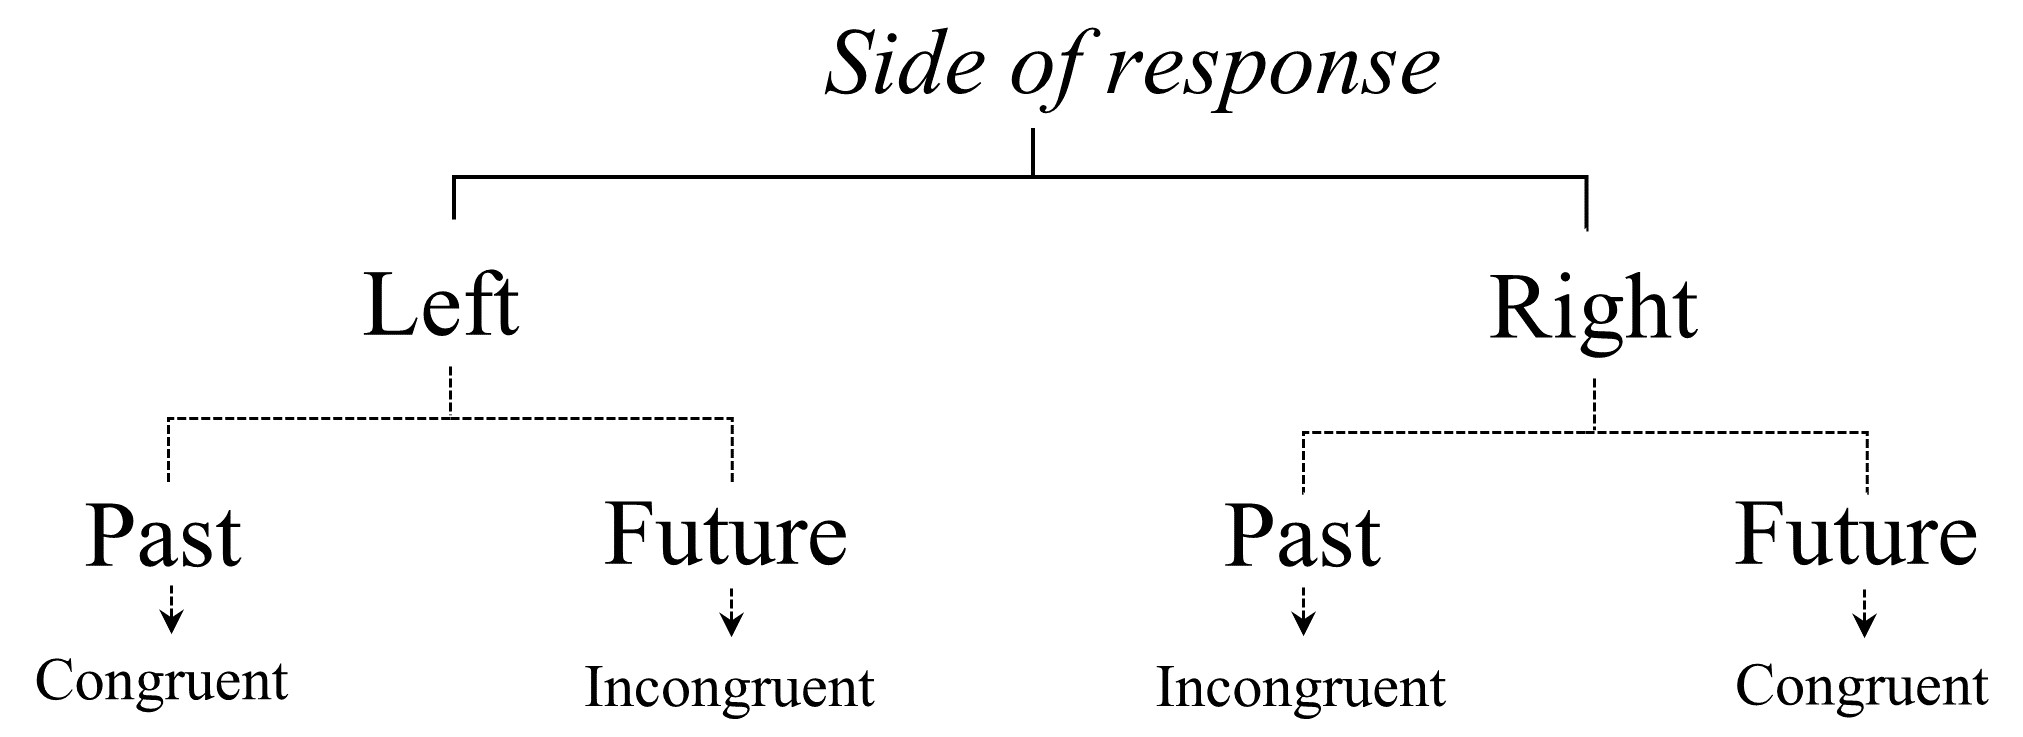
\includegraphics[width=0.8\linewidth]{figures/chap-3-fig1} 

}

\caption{Schematic Description of the Basic Design for Yes-Responses (Words). Note: Past-tense words that require a left-side response and future-tense words that require a right-side response are congruent with the mental timeline. When the same words require responses on the opposite side, they become incongruent (i.e., past to the right and future to the left).}\label{fig:chap-3-fig1}
\end{figure}

\hypertarget{apparatus}{%
\paragraph{Apparatus}\label{apparatus}}

Stimuli were displayed on a 15-inch LCD screen in black 37-point monospaced fonts (droid sans mono) on a grey background. The experiment was created using OpenSesame {[}Version 3.2.6. ; \protect\hyperlink{ref-mathot_opensesame_2012}{Mathôt et al.} (\protect\hyperlink{ref-mathot_opensesame_2012}{2012}){]}. Participants used their right (dominant) hand to move a pen to the right or to the left of a trackpad for the ``yes''/''no'' decision (Genius EasyPen 340). The left and right response areas of the trackpad were spatially delimited by a virtual boundary (+/-700 pixels from the centre on the trackpad, for the left and right responses, respectively). Yes- and no-responses to the left and right side on the trackpad were counterbalanced across conditions and participants, that is, during half of the experiment, participants were instructed to move the pen towards one side of the trackpad for real words (``yes'' responses) and to the opposite side for pseudowords (``no'' response) and, after a short pause, the word/pseudoword responses sides were reversed. To restrict movement only to the wrist and reduce movement variability across trials and participants, participants placed their right hand on a wrist rest.

\hypertarget{procedure}{%
\paragraph{Procedure}\label{procedure}}

The experiment was run in a quiet testing room. Participants completed the Edinburgh Handedness Inventory (\protect\hyperlink{ref-oldfield_assessment_1971}{Oldfield, 1971}) and received instructions in written and oral form. They were instructed to decide as rapidly and as accurately as possible whether the stimulus was a French word or not by moving the pen towards the left or right side of the trackpad (see Figure \ref{fig:chap-3-fig2}). Half of the participants started with ``yes'' responses towards the left of the trackpad, half of the participants started with ``yes'' responses towards the right. The direction of response was reversed during the second part of the experiment for all participants. Participants were trained before the beginning of the experiment, as well as halfway through. They started the experiment after reaching a threshold of 80\% correct responses during training (approximately 30 trials). Each participant saw a total of 80 words and 80 pseudowords randomized in two counterbalanced blocks (``yes'' to the right and ``yes'' to the left). When the ``yes'' response was to the right, future-tense words were congruent and past-tense words were incongruent (see Figure \ref{fig:chap-3-fig1}). In this block, 20 words were future-congruent and 20 words were past-incongruent (i.e., total of 40 words per block, 20 words per condition). When the ``yes'' response was to the left, past-tense words were congruent and future-tense words were incongruent. In this block, we had 20 past-congruent and 20 future-incongruent words (i.e., total of 40 words per block, 20 words per condition). This design allowed us to present each stimulus in the past or future tense, during the first or the second part of the experiment, and in congruent or incongruent conditions.

\begin{figure}[htbp!]

{\centering 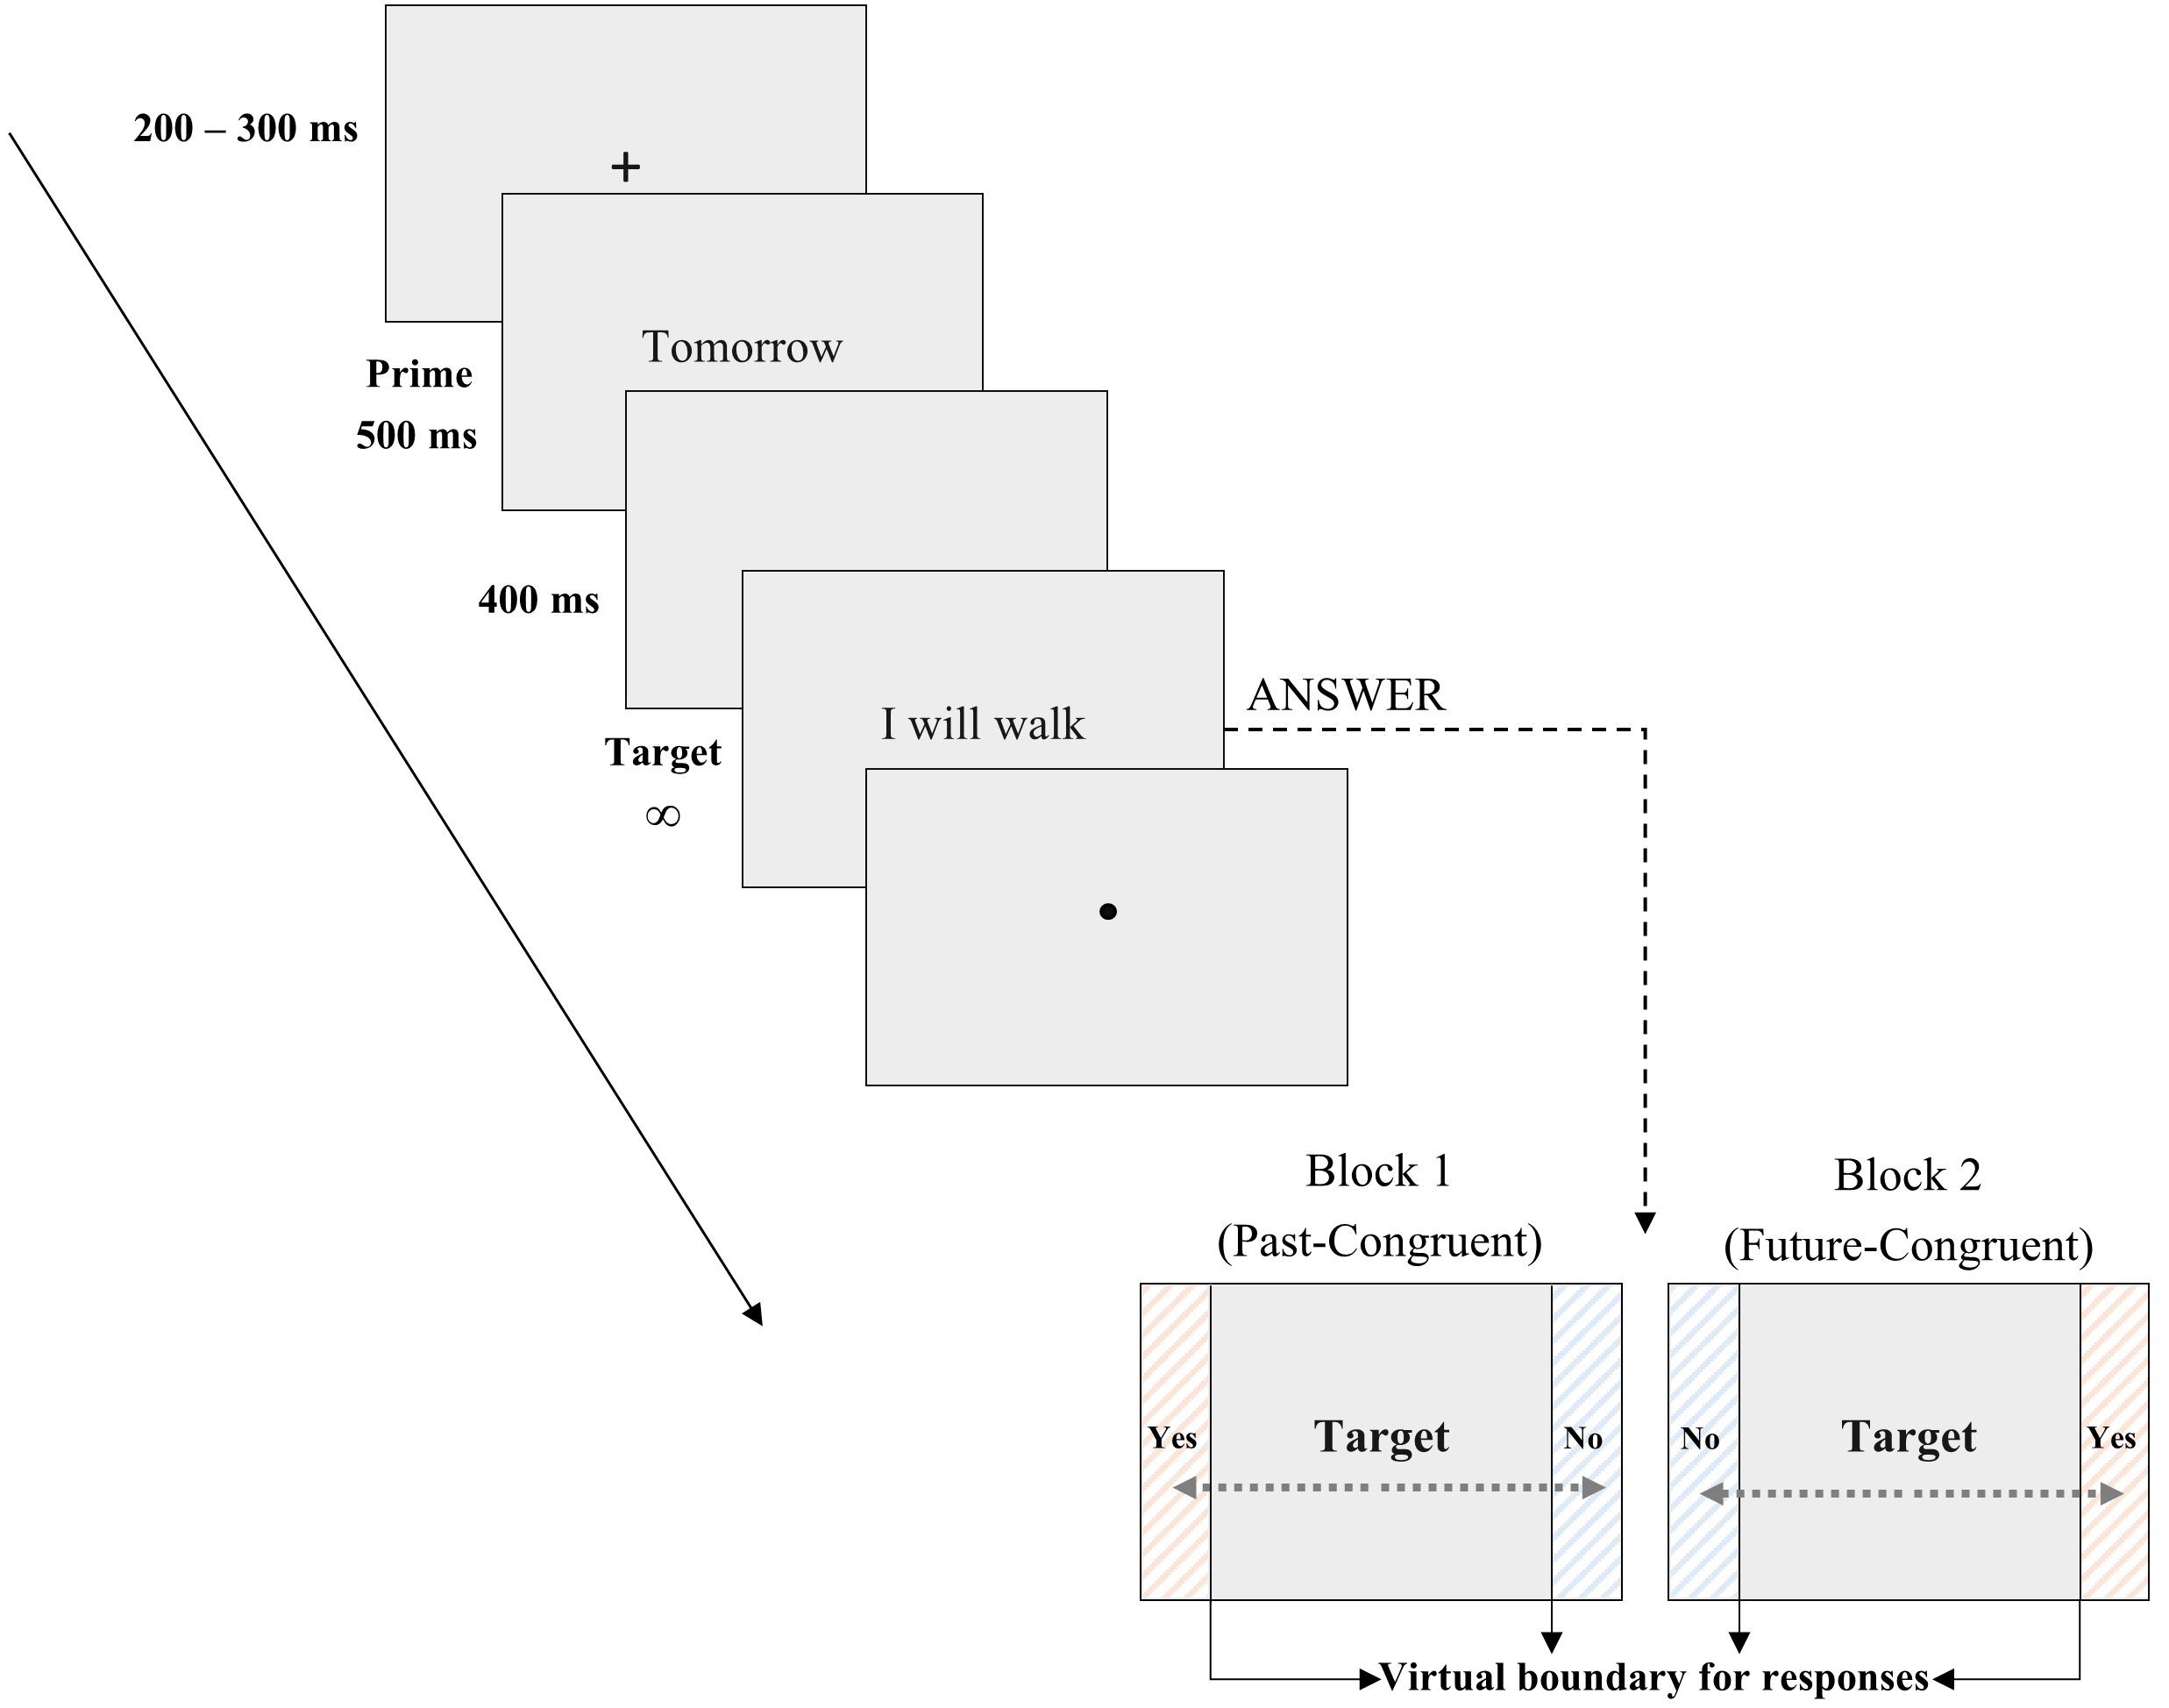
\includegraphics[width=1\linewidth]{figures/chap-3-fig2} 

}

\caption{Task Design of Experiment 1. Note: After the fixation cross, a prime (“yesterday” or “tomorrow”) was displayed, followed by a real target word or pseudoword. Participants made their lexical decision after the onset of the target by moving their pen on the trackpad towards the left or right. To start a new trial, participants had to replace the pen at the center of the trackpad (indicated by a black dot). Target words and pseudowords remained on the screen until a response was made.}\label{fig:chap-3-fig2}
\end{figure}

The experiment started once the training session was completed. As can be seen in Figure \ref{fig:chap-3-fig2}, at the beginning of each trial, a fixation cross was displayed in the centre of the screen for a duration that varied randomly between 200 and 300 ms, followed by a prime for 500 ms, a blank display for 400 ms and then the target (e.g., I walked). In order to reinforce the salience of temporal information, each target was preceded by a congruent prime, that is, all past-tense words and pseudowords were primed by ``Yesterday'' and all future-tense words and pseudowords were primed by ``Tomorrow.'' Targets stayed on the screen until the response of the participant, that is until the pen crossed the virtual boundary of the response area. Therefore, response times corresponded to the time needed to reach the boundary after the onset of the target. After the response, participants were required to replace the pen at the centre (represented by a black dot) before each new trial. The pen had to be at the centre to start a new trial. If the participants responded too slowly, a beep was played after 1000ms (post target onset). In between the blocks (after 80 trials), participants had a 2-minute break, and they were instructed to change the response direction for ``yes''/''no'' decisions. They started a new training phase before completing the second part of the experiment.

\hypertarget{data-analyses}{%
\paragraph{Data analyses}\label{data-analyses}}

The data were analyzed using both standard analyses of variance (ANOVA) with either participants (F1) or items (F2) as the random variables and linear mixed effect models with participants and items as crossed random effects (\protect\hyperlink{ref-baayen_mixed-effects_2008}{Baayen et al., 2008}; \protect\hyperlink{ref-barr_random_2013}{Barr, 2013}). For the ANOVAs, we used a 2 × 2 within-participant ANOVA with Side and Time as factors. Note that the congruency effect is the interaction between Side and Time. That is, when the side of the response for a past-tense word (e.g., he walked) changes from left to right, the word stops being congruent and, instead, becomes incongruent. Similarly, when the side of the response for a future-tense word (e.g., he will walk) changes from left to right, the word stops being incongruent and becomes congruent (see Figure \ref{fig:chap-3-fig1}).

For the linear mixed-effect analyses, latency data were fitted with lmer and accuracy data with glmer functions from the \texttt{lme4} package (\protect\hyperlink{ref-R-lme4}{Bates et al., 2018}) in the \texttt{R} statistical computing environment (Version 3.5.2, \protect\hyperlink{ref-R-base}{R Core Team, 2018}). We report unstandardized regression coefficients, standard errors (\emph{SEs}), and \emph{t} values (for lmer) or \emph{z} values (for \texttt{glmer}). Fixed effects were deemed reliable if \textbar t\textbar{} or \textbar z\textbar{} was greater than 1.96 (\protect\hyperlink{ref-baayen_analyzing_2008}{Baayen, 2008}). We used the maximal random structure model that reached convergence (\protect\hyperlink{ref-barr_random_2013}{Barr, 2013}), and this included by-participant and by-item random intercepts in all analyses that we report. Fixed effects, random effects, and random slopes were only included if they significantly improved the model's fit in a forward stepwise model selection procedure. Models were selected using chi-squared log-likelihood ratio tests with regular maximum likelihood parameter estimation. Following the procedure described by \protect\hyperlink{ref-brysbaert_power_2018}{Brysbaert \& Stevens} (\protect\hyperlink{ref-brysbaert_power_2018}{2018}), we conducted power analysis based on 1000 simulations with \texttt{powerSim} functions from the \texttt{simR} package (\protect\hyperlink{ref-green_simr_2016}{Green \& MacLeod, 2016}).

\hypertarget{results}{%
\subsubsection{Results}\label{results}}

We analyzed the reaction time (RTs) of correct responses and error rates (ER) for 39 participants. Statistical analyses were conducted separately for words and pseudowords. We first removed extreme values (i.e., RTs below 250 ms or above 4000 ms), then we considered as outliers data points that were above or below 2.5 standard deviations from each individual participant's mean RT. Outliers were replaced by the cut-off RT corresponding to each participant's mean +/- 2.5 standard deviation (\protect\hyperlink{ref-hoaglin_performance_1986}{Hoaglin et al., 1986}).

\hypertarget{words}{%
\paragraph{Words}\label{words}}

The results for the word trials are shown in Figure \ref{fig:chap-3-fig3}. We conducted a 2 × 2 within-participant ANOVA, which resulted from the factorial combination of the effects of Side (left versus right) and Time (past vs.~future).

As concerns RTs, the ANOVA showed no significant main effect of Time, \emph{F1}(1, 38) = .49, \emph{p} \textgreater{} .49 and \emph{F2} (1, 79) = 2.16, \emph{p} \textgreater{} .14, or Side, \emph{F1}(1, 38) = 2.44, \emph{p} \textgreater{} .12 and \emph{F2} (1, 79) = 2.77, \emph{p} \textgreater{} .10, but a highly significant interaction between the effects of Time and Side, \emph{F1}(1, 38) = 12.59, \emph{p} \textless{} .001 and \emph{F2} (1, 79) = 12.232, \emph{p} \textless{} .001. As explained above, the significant interaction reflects the congruency effect. That is, when the side of the response for a past-tense word (I walked) changes from left to right, the word becomes spatially inconsistent (i.e., incongruent). By contrast, when the side of the response for a future-tense word (I will walk) changes from left to right, the word becomes spatially consistent (i.e., congruent). The interaction results from the fact that congruent words were generally responded to more quickly than incongruent words.

In the mixed effect analyses of RT data, the final model included Time, Side, Block and the interaction between Time and Side as fixed effects. As random effects, we had by-participant and by-item intercepts, random slopes for side, and random slopes for time by-participants. The results showed a significant effect of Time (\emph{b} = 37.927, \emph{SE} = 9.48, \emph{t} = 4.00), Side (\emph{b} = 35.717, \emph{SE} = 14.27, \emph{t} = 2.50), and a significant interaction between Time and Side (\emph{b} = -52.181, \emph{SE} = 10.79, \emph{t} = 4.84). There was also an effect of Block (\emph{b} = -21.410, \emph{SE} = 11.34, \emph{t} = 1.89), which reflected the fact that participants were faster in the second block but this effect did not interact with the effects of interest. Contrast analyses showed that participants were faster to respond for congruent than for incongruent words (\emph{b} = -36.034, \emph{SE} = 14.81, \emph{t} = 2.43), and this congruency effect did not interact with Time (\emph{b}= 20.336, \emph{SE} = 27.62, \emph{t} = 0.74). The power of this last model (i.e., congruency and time) in 1000 simulated studies was .78, 95\% CI = {[}76.24, 81.39{]}.

As concerns response accuracy (ERs), the ANOVA showed a significant main effect of Time (past vs.~future), \emph{F1}(1, 38) = 9.13, \emph{p} \textless{} .01 and \emph{F2} (1, 79) = 11.44, \emph{p} \textless{} .001, reflecting the fact that past-tense words yielded higher error rates than future-tense words. The main effect of Side (left v. right) was not significant, \emph{F1}(1, 38) = .18, \emph{p} \textgreater{} .50 and \emph{F2}(1, 79) = .71, \emph{p} \textgreater{} .40. The critical interaction between the effects of Time and Side (congruency effect) failed to reach significance, \emph{F1}(1, 38) = 2.24, \emph{p} \textgreater{} .15 and \emph{F2} (1, 79) = 3.41, \emph{p} = .069.

In the mixed effect analyses of accuracy data, the final model included Time, Side and their interaction as fixed effects. As random effects, we had random intercepts for participants and items. As in the ANOVA analyses, there was a significant effect of Time (\emph{b} = -0.852, \emph{SE} = 0.22, \emph{z} = 3.91) and a marginally significant interaction between Side and Time (\emph{b} = 0.570, \emph{SE} = 0.30, \emph{z} = 1.88). Contrast analysis of this interaction showed that participants made more errors in the incongruent condition than in the congruent condition (\emph{b} = 0.516, \emph{SE} = 0.22, \emph{z} = 2.31). No other effects were significant. The power of this last model (i.e., congruency and time) in 1000 simulated studies was .67, 95\% CI = {[}64.09, 70.01{]}.

\begin{figure}[htbp!]

{\centering 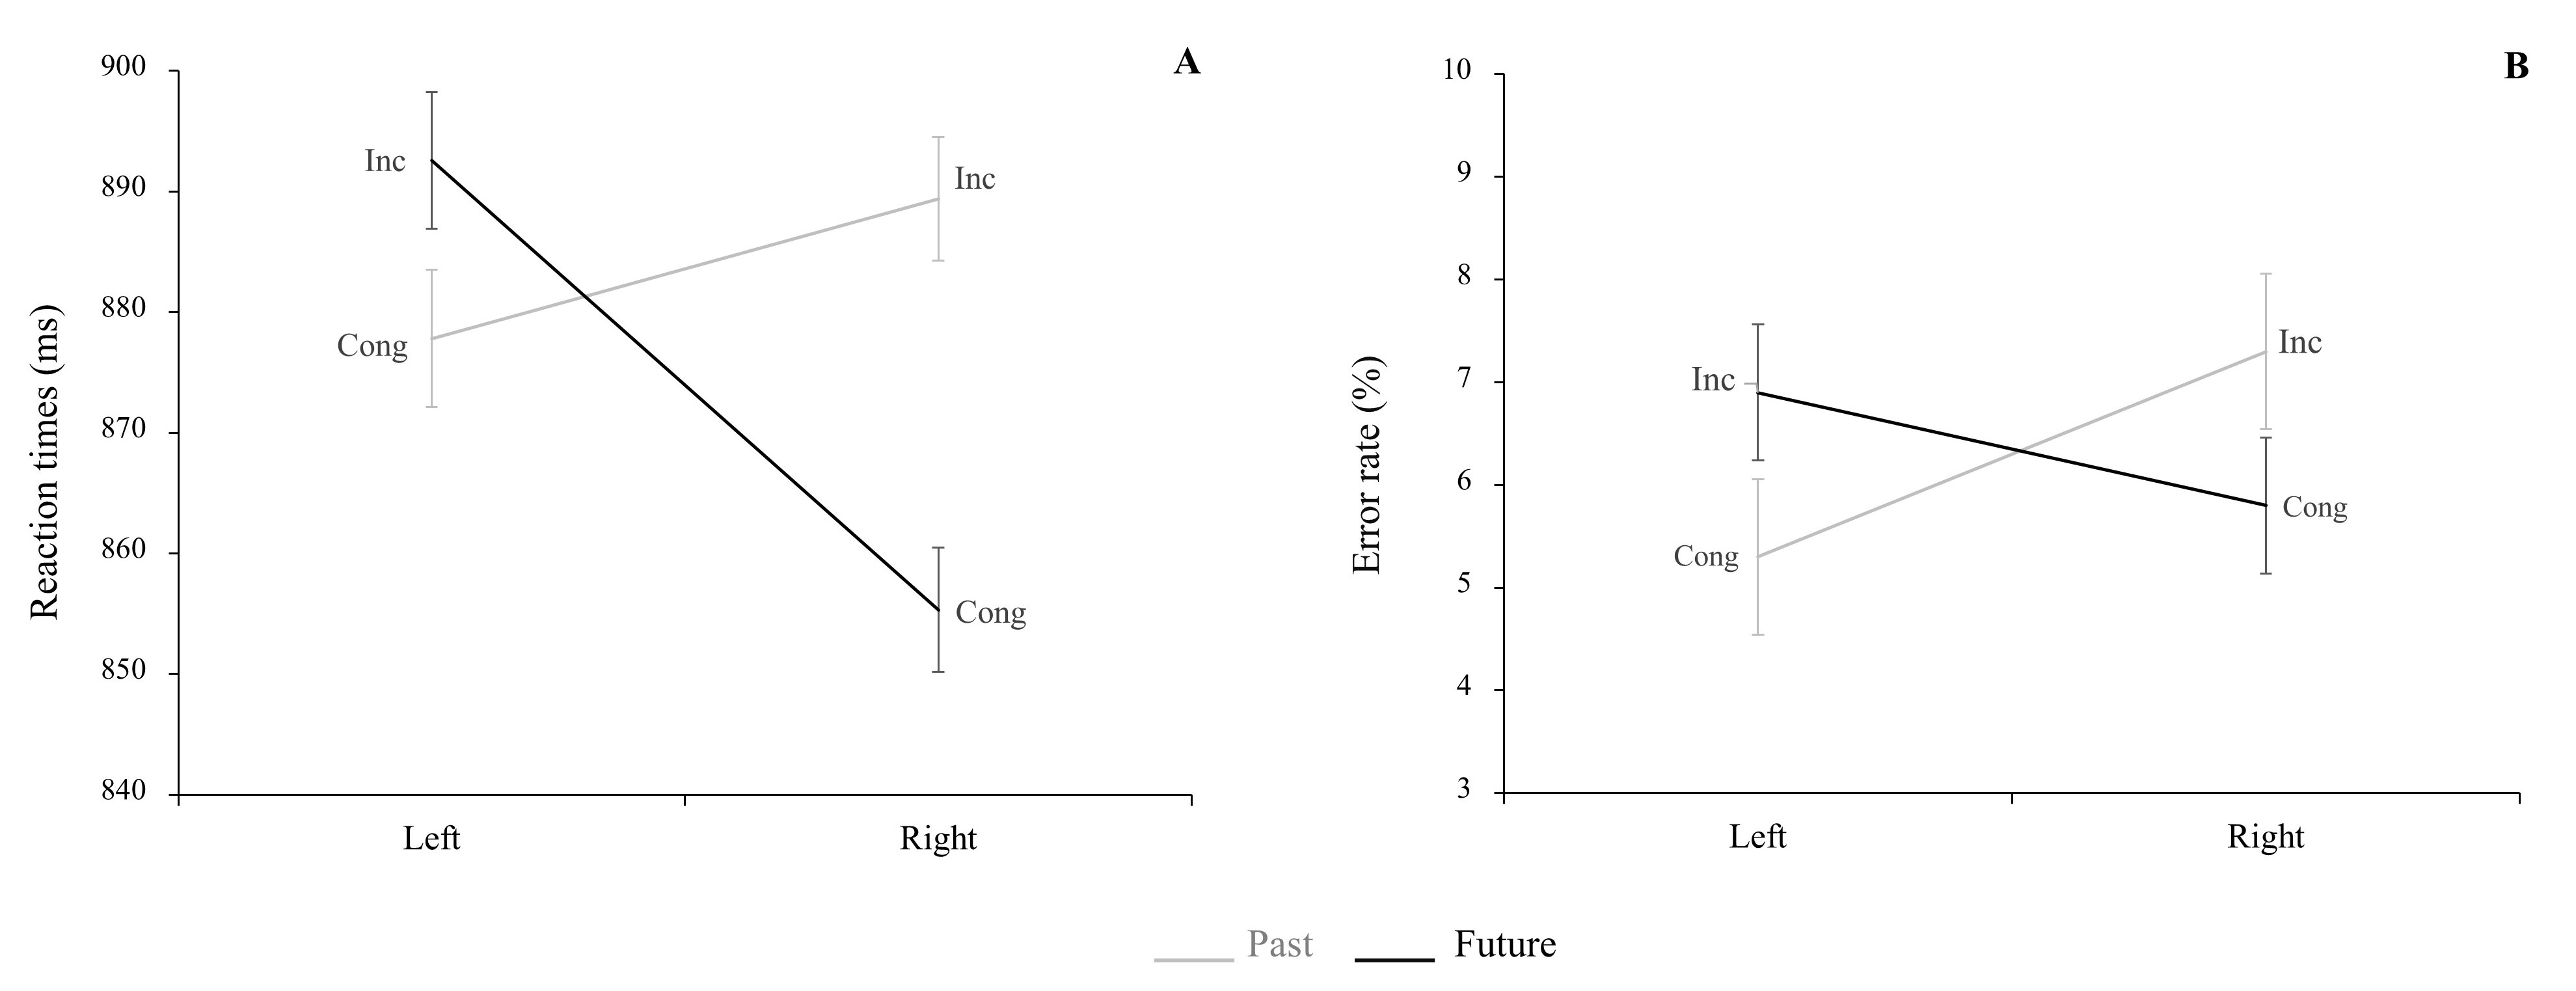
\includegraphics[width=1\linewidth]{figures/chap-3-fig3} 

}

\caption{Experiment 1: Mean Reaction Times (A) and Mean Error Rates (B) as a Function of Response Side (Left Versus Right) and Verb Tense (Past Versus Future). Note : Inc = incongruent; Cong = congruent. Mean errors were normalized for tense for the graphical representation of the congruency effect. Error bars indicate within-participant standard errors.}\label{fig:chap-3-fig3}
\end{figure}

\hypertarget{pseudowords}{%
\paragraph{Pseudowords}\label{pseudowords}}

Responses to three pseudowords where excluded from the analyses because of high error rates (between 38\% and 89\%).

As concerns RTs, the ANOVA showed no significant effects of Side (\emph{Fs} \textless{} 1), Time (\emph{F1}(1, 38) = 2.09, p \textgreater{} .15 and \emph{F2} (1, 76) = 1.49, \emph{p} \textgreater{} .20) and no significant interaction between the effects of Side and Time (\emph{Fs} \textless{} 1). The final linear mixed model for the RT data included Side, Time and their interaction, as well as block (Part1 vs Part2). As random effects, we had by-participants and by-items random intercepts, and by-participants random slopes for the effect of tense and side. Participants were faster during the second block of the experiment (\emph{b} = -32.620, \emph{SE} = 10.00, \emph{t} = 3.26). No other significant effects were obtained.

As concerns accuracy data, the ANOVA revealed a significant effect of Time \emph{F1}(1, 38) = 5.63, \emph{p} \textless{} .05 and \emph{F2} (1, 76) = 2.35, \emph{p} \textgreater{} .14, but no effect of Side (\emph{Fs} \textless{} 1) and no significant interaction between the effects of Time and Side \emph{F1}(1, 38) = 2.18, \emph{p} \textgreater{} .14 and \emph{F2} (1, 76) = 1.16, \emph{p} \textgreater{} .25. The final linear mixed effect model of the accuracy data included Side, Time and their interaction. As random effects, we had intercepts for subjects and items, as well as by-items random slopes for the effect of tense. A marginally significant effect of Time was obtained reflecting the fact participants made more errors for past-tense than future-tense pseudowords (\emph{b} = 0.436, \emph{SE} = 0.23, \emph{z} = 1.89). No other effect was significant.

\hypertarget{discussion}{%
\subsubsection{Discussion}\label{discussion}}

In line with our prediction, we found a significant space-time congruency effect in visual word recognition. Lexical decision movements that were incongruent with the mental timeline resulted in an increase in reaction times and to some extent ERs. That is, participants were slower when they had to move to the right for words that referred to past events and to the left for words that referred to future events. Although the effects went in the same direction for ERs (more errors for incongruent words), the critical time by space interaction failed to reach significance. However, the absence of a significant effect on errors is not necessarily a problem. In response-limited conditions (i.e., when stimuli are unmasked, presentation time is unlimited and performance is typically high), the critical dependent variable is latency not ERs (\protect\hyperlink{ref-grainger_orthographic_1996}{Grainger \& Jacobs, 1996}). Indeed, in the lexical-decision task, most psycholinguistic effects in skilled adult readers show up on latencies rather than ERs (\protect\hyperlink{ref-coltheart_drc_2001}{Coltheart et al., 2001}). Not surprisingly, the dominant models of the lexical-decision task are concerned with explaining response time distributions rather than errors (e.g., \protect\hyperlink{ref-dufau_how_2012}{Dufau et al., 2012}; \protect\hyperlink{ref-ratcliff_diffusion_2004}{Ratcliff et al., 2004}).
Our results join those of \protect\hyperlink{ref-sell_processing_2011}{Sell \& Kaschak} (\protect\hyperlink{ref-sell_processing_2011}{2011}) to suggest that the processing of temporal information in the language domain automatically activates the mental timeline, which interferes with movement through space. The fact that the congruency effect was only found for words but not for pseudowords suggests that this effect was generated by time-relevant information stored in lexical representations and not by sublexical processes.

An important issue remains to be addressed. Several studies have failed to find a space-time congruency effect along the left-right axis when temporal information was not relevant to the task (e.g., \protect\hyperlink{ref-maienborn_we_2015}{Maienborn et al., 2015}; \protect\hyperlink{ref-ulrich_leftright_2010}{Ulrich \& Maienborn, 2010}; \protect\hyperlink{ref-von_sobbe_space-time_2019}{von Sobbe et al., 2019}); leading these authors to conclude that the mental timeline is not automatically activated during semantic processing of concepts related to time and, instead, reflects facilitated memory access rather than automatic sensorimotor activation (\protect\hyperlink{ref-maienborn_we_2015}{Maienborn et al., 2015}; \protect\hyperlink{ref-von_sobbe_space-time_2019}{von Sobbe et al., 2019}). One of the key differences between studies that found space-time congruency effects and those that failed to find these effects is the involvement of movement. Indeed, Maienborn and colleagues (\protect\hyperlink{ref-maienborn_we_2015}{Maienborn et al., 2015}; \protect\hyperlink{ref-ulrich_leftright_2010}{Ulrich \& Maienborn, 2010}) used static and lateralized hand responses (e.g., a button press with the right hand to indicate the future and a button press with the left hand to indicate the past), whereas \protect\hyperlink{ref-sell_processing_2011}{Sell \& Kaschak} (\protect\hyperlink{ref-sell_processing_2011}{2011}) found a congruency effect only for an arm movement condition but not for a static button-press condition (for a replication, see also \protect\hyperlink{ref-scheifele_replication_2018}{Scheifele et al., 2018}). This suggests that movement might be the key component underlying the spatial organization of the mental timeline and its functional role during semantic processes of grammatical time (past/future). Experiment 2 was designed to replicate our results and further investigate the importance of movement for the occurrence of space-time congruency effects in word recognition.

\hypertarget{experiment-2}{%
\subsection{Experiment 2}\label{experiment-2}}

Experiment 2 was designed to replicate the results found in Experiment 1 and to directly assess the role of movement in the space-time congruency effect. To this end, the same space-time manipulation was used, but participants had to respond either with a trackpad or mouse, both of which required lateral movement through space, or a lateralized keypress, which did not. If spatially directed movement were the key component of the space-time compatibility effect, we would expect a space-time compatibility effect only in the movement conditions.

In addition, we tested whether rendering the temporal information more salient by using a prime is a necessary condition to obtain significant space-time compatibility effects. In Experiment 1, a prime (yesterday/tomorrow) was systematically and consistently associated with the subsequent verb, which reinforced the temporal context and created a minimal syntactic structure (Tomorrow I will walk) that might have amplified the effects. Thus, in Experiment 2, we decided to systematically manipulate the presence of a prime in half of the trials.

To increase the power of the experiment, and as a consequence of the 2020 coronavirus-related lockdown in France, we opted for an online experiment that yielded data from more than 1,100 students from Aix-Marseille University.

\hypertarget{methods-1}{%
\subsubsection{Methods}\label{methods-1}}

\hypertarget{participants-1}{%
\paragraph{Participants}\label{participants-1}}

A total 1,104 students from Aix-Marseille University participated in our online experiment. The experiment was advertised through a mailing list to all university students. Students were free to participate and data collection was totally anonymous. To motivate a large number of students to participate in the experiment, they were informed that a number of participants (1:50) were randomly drawn to receive a monetary reward of 50 euros for their participation.

Because the data from online experiments are much noisier than laboratory experiments, we first cleaned the data, which resulted in the exclusion of 44 participants who had incomplete data or gave aberrant responses: 26 participants did not report the type of device they used for responding (i.e., trackpad or mouse), 7 participants had ERs above 75\% suggesting they had inverted response mappings, and 11 participants repeatedly answered using the same response side. We then removed aberrant RTs (see the results section for more details) and calculated the mean RT and 2.5 standard deviations from the mean for all participants. We then excluded 42 participants whose mean RTs were more than 2.5 standard deviations above or below the mean of the group. Overall, this exclusion procedure left us with the data from 1018 participants that were included in the final analysis. To simplify the procedure and instructions for this online experiment, in Experiment 2 we did not ask participants to change the side of yes-responses halfway through the experiment. Therefore, for half of the participants, the yes-response was always on the left side, and for the other half, the yes-response was always on the right side.

The participants were on average 23 years-old (\emph{SD} = 5.3, ranging from 17 to 64 years old), 642 were female, 887 were right-handed, 110 were left-handed, and 21 were ambidextrous. Two hundred ninety-four participants did the experiment using a trackpad (150 responded ``yes'' to the right and 144 responded ``yes'' to the left), 208 participants used a mouse (118 left yes responses and 90 right yes responses), and 516 participants did the experiment using a keyboard (251 left yes responses and 265 right yes responses).

\hypertarget{stimuli-and-apparatus}{%
\paragraph{Stimuli and Apparatus}\label{stimuli-and-apparatus}}

The stimuli were identical to those of Experiment 1. The experiment was programmed using PHP, JAVASCRIPT and HTML. Participants were asked to either use the keyboard, mouse or trackpad. For the keyboard, participants gave their response by pressing the `Q' key for left answers and `M' for right answers (azerty keyboard) with their left and right index fingers. For the mouse or trackpad, participants moved their mouse or their finger on the trackpad toward to the left-or-right side of space using their dominant hand. A virtual boundary was placed 10\% to the left and 10\% to the right of both edges to detect yes and no responses.

\hypertarget{design-and-procedure}{%
\paragraph{Design and Procedure}\label{design-and-procedure}}

The design was almost identical to that of Experiment 1 with four notable exceptions. First, participants were asked to respond either with a mouse or trackpad (movement) or with a keyboard (no movement). Second, the side of the response was fixed for a given Participant to avoid participants having to change response sides halfway through the experiment. Third, half of the trials were preceded by a congruent prime word, (i.e., ``yesterday'' for past tense stimuli and ``tomorrow'' for future tense stimuli) and the other half were preceded by a black square (no priming). Fourth, a 400-ms feedback stimulus was added to the end of the trial (i.e., a green cross for correct responses or a red cross for incorrect responses) to maintain participants' motivation and a beep was played 1,500 ms after target onset to discourage slow responses.

When opening the web link of the online experiment, each participant was assigned at random to either a movement condition (trackpad our mouse) or a no-movement condition (keyboard) and to a response side (yes responses to the left or yes responses to the right). Participants were instructed to decide as rapidly and as accurately as possible whether the stimulus was a French word or not. The sides to which yes responses were made were counterbalanced across participants. Participants were asked to perform the experiment in a quiet environment with no acoustic and visual distractions. They started the experiment after completing a questionnaire (i.e., age, gender, education level, dominant hand and device used) and a short training of 20 trials.

\hypertarget{analyses}{%
\paragraph{Analyses}\label{analyses}}

The procedure for data analyses was identical to that of Experiment 1.

\hypertarget{results-1}{%
\subsubsection{Results}\label{results-1}}

We analyzed RTs for correct responses and response accuracy (ERs) for 1018 participants. After visual inspection of the RT distributions, we first removed extreme RTs that were below 300 ms and above 3,000 ms for the trackpad, below 250 ms and above 3,000 ms for the mouse and below 250 ms and above 2,500 ms for the keyboard. Then, we identified outliers that were beyond 2.5 standard deviations from the individual mean RT and we winsorized these data points (\protect\hyperlink{ref-hoaglin_performance_1986}{Hoaglin et al., 1986}). The average RTs and ERs for each condition are shown in Figure \ref{fig:chap-3-fig4}. Statistical analyses were conducted separately for words and pseudowords.

\hypertarget{words-1}{%
\paragraph{Words}\label{words-1}}

Two sets of ANOVAs were conducted with subjects (\emph{F1}) and items (\emph{F2}) as random variables. In the \emph{F1} analyses, device (trackpad, mouse, keyboard) and side (left vs.~right) were between-subjects factors and time (past vs.~future) and prime (with, without) were within-subject factors. In the \emph{F2} analyses, all factors were within-item because every word stem had been seen in every condition.

The ANOVA analysis of RT data showed significant main effects of device, \emph{F1}(2, 1012) = 243.88, \emph{p} = .001; \emph{F2}(2, 158) = 5436.91, \emph{p} = .001; side, \emph{F1}(1, 1012) = 15.38, \emph{p} = .001; \emph{F2}(1, 79) = 368.14, \emph{p} = .001; and prime, \emph{F1}(1, 1012) = 80.71, \emph{p} = .001; \emph{F2}(1, 79) = 56.53, \emph{p} = .001. Time was not significant (Fs , 1). Importantly, the congruency effect, which is the interaction between time and side, was highly significant, \emph{F1}(1, 1012) = 30.18, \emph{p} = .001; \emph{F2}(1, 79) = 17.23, p , .001. Moreover, the triple interaction between time, side, and device was significant by participants but not by items, \emph{F1}(2, 1012) = 3.02, \emph{p} = .05; \emph{F2}(1, 79) = 1.78, \emph{p} = .15, which indicates that the congruency effect was modulated by device. Indeed, when we combined the two movement conditions (trackpad and mouse) and contrasted them with the no-movement condition (keyboard), the triple interaction between time, side, and movement was significant by participants and by items, \emph{F1}(2, 1014) = 6.57, \emph{p} = .05; \emph{F2}(1, 79) = 4.17, \emph{p} = .05, which indicated that the congruency was larger in the movement conditions than in the no-movement condition (see more detailed analyses below). Prime did not affect the congruency effect, that is the triple interaction between time, side and device was not significant (\emph{Fs}, 1). Prime only interacted with Device {[}\emph{F1}(2, 1012) = 7.72, \emph{p} \textless{} .001; \emph{F2}(2, 158) = 3.87, p \textless{} .05{]}, reflecting the fact that the priming effects were larger for devices that produced longer RTs (mouse and trackpad).

As concerns the mixed effect analysis of the RT data, the final model included Time (past vs future), Side (left vs right), Device (i.e., trackpad, mouse or keyboard), Prime (i.e., with or without) and their interaction, by-participant and by-item random intercepts, and a random slope for prime by-participants. Results showed a significant effect of Time (\emph{b} = 23.482, \emph{SE} = 5.10, \emph{t} = 4.60), Side (\emph{b} = 50.576, \emph{SE} = 13.866, \emph{t} = 3.65), Device (\emph{b} = -84.666, \emph{SE} = 6.57, \emph{t} = 12.89), and Prime (\emph{b} = -30.516, \emph{SE} = 7.09, \emph{t} = 4.30). Moreover, results revealed that device interact significantly with Time (b = -13.573, SE = 3.7, \emph{t} = 4.03) and with Prime (\emph{b} = -9.539, \emph{SE} = 3.49, \emph{t} = 2.73). Importantly, as in the ANOVA analyses, the critical interaction between Side and Time (i.e., the congruency effect) was significant (\emph{b} = -30.516, \emph{SE} = 7.09, \emph{t} = 4.30) and this congruency effect was modulated by Device, as seen in a three-way interaction between Side, Time and Device (\emph{b} = 12.016, \emph{SE} = 4.75, \emph{t} = 2.53). No other effect was significant. Given that this three-way interaction was significant, we conducted separate analyses for each condition (i.e., trackpad, mouse and keyboard).

\begin{landscape}

\begin{figure}[htbp!]

{\centering 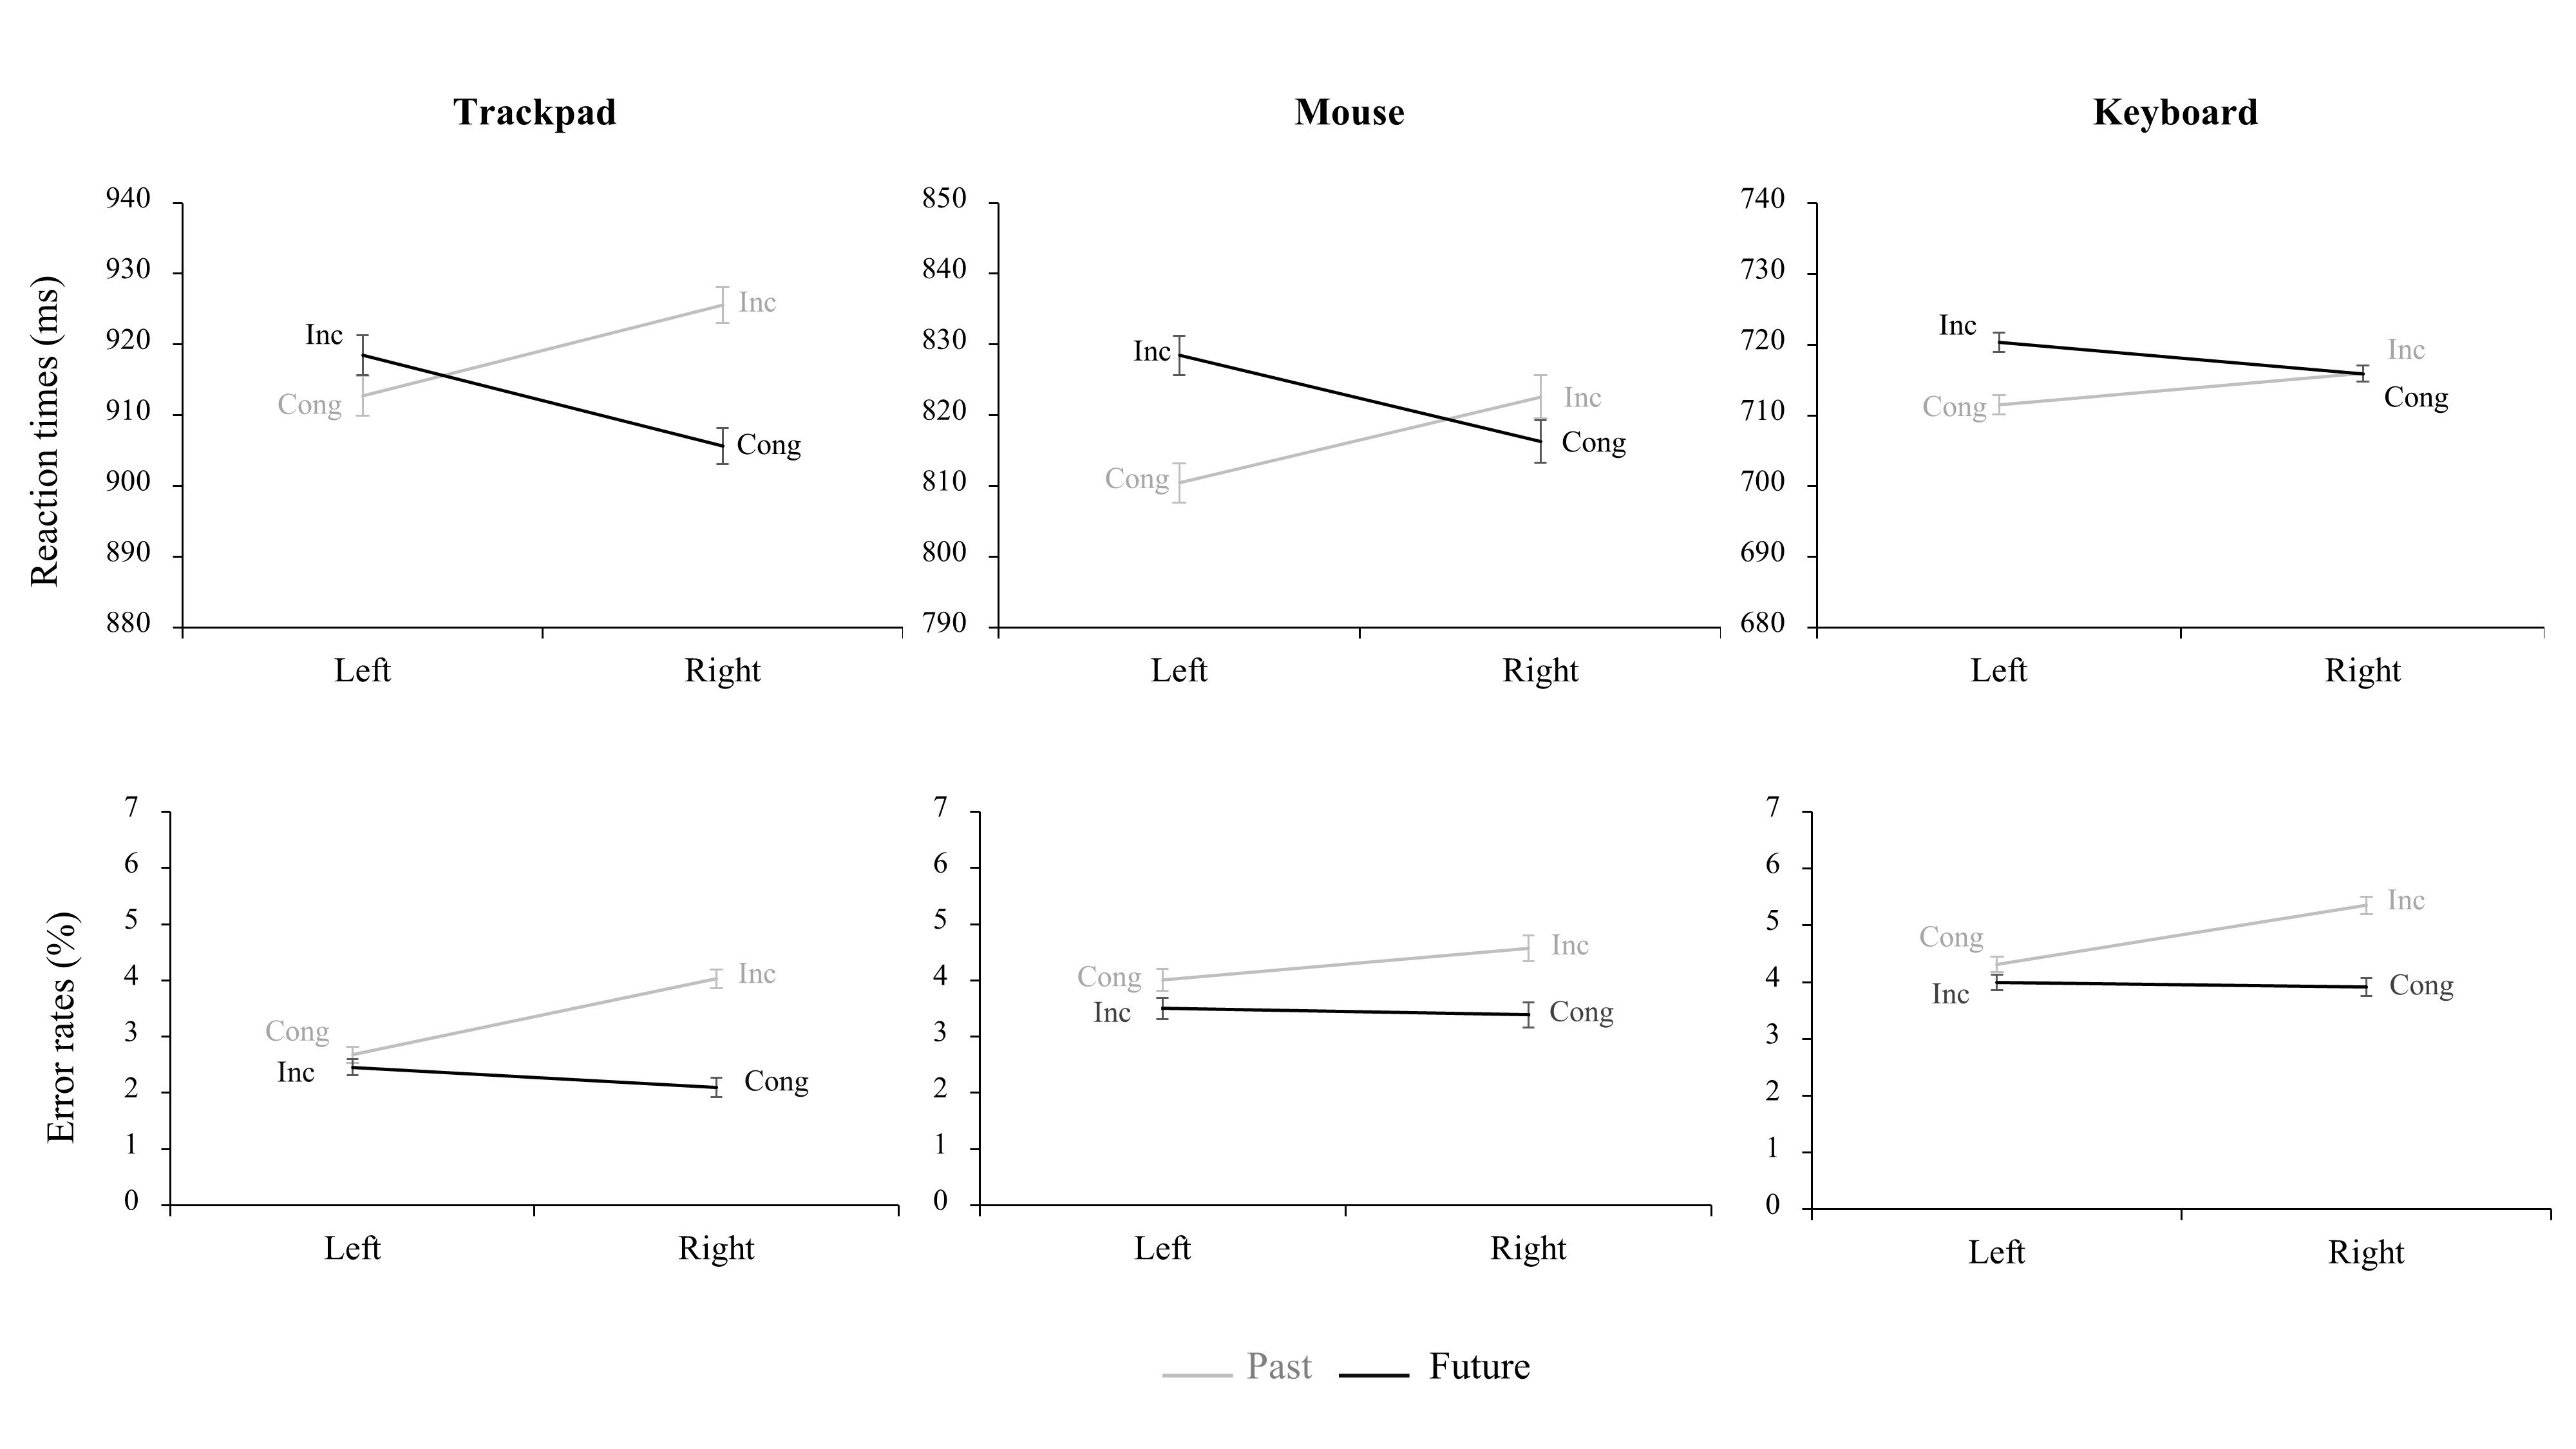
\includegraphics[width=0.9\linewidth]{figures/chap-3-fig4} 

}

\caption{Experiment 2: Mean Reaction Times and Mean Error Rates as a Function of Response Side (Left Versus Right), Verb Tense (Past Versus Future), and Movement (Trackpad Versus Mouse Versus Keyboard). Note : Because the group of participants who responded to the right was globally faster than the group that responded to the left, we normalized the RTs for side. Note that this normalization only affects the visual presentation of the results but not the statistical significance of the congruency effect. Error bars indicate within-participant standard errors.}\label{fig:chap-3-fig4}
\end{figure}

\end{landscape}

\hypertarget{trackpad}{%
\subparagraph{Trackpad}\label{trackpad}}

The final model included Time (past vs future), Congruency (congruent vs congruent), Prime (i.e., with and without) and their interaction, by-participant and by-item random intercepts, and random slopes for tense by-participants and by-items. Results showed significant effects of Congruency (\emph{b} = -40.573, \emph{SE} = 17.65, \emph{t} = 2.30) and Prime (\emph{b} = 25.462, \emph{SE} = 6.26, \emph{t} = 4.07). Importantly, the prime effect did not interact with congruency effect (\emph{b} = -0.850, \emph{SE} = 8.94, \emph{t} = 0.09). The power of this model in 1000 simulated studies was .89, 95\% CI = {[}87.22, 91.15{]}. No other effect was significant.

\hypertarget{mouse}{%
\subparagraph{Mouse}\label{mouse}}

The final model included Time (past vs future), Congruency (congruent vs congruent), Prime (i.e., with and without) and their interaction, by-participants and by-items random intercepts, and random slopes for tense by-participants and by-items. Results showed significant effects of Time (\emph{b} = -64.882, \emph{SE} = 19.91, \emph{t} = 3.26), Congruency (\emph{b} = -66.632, \emph{SE} = 20.27, \emph{t} = 3.29) and Prime (\emph{b} = 14.581, \emph{SE} = 6.45, \emph{t} = 2.26). As for trackpad experiment, the prime effect did not interact with the congruency effect (\emph{b} = 3.87, \emph{SE} = 9.89, \emph{t} = 0.52) or with Time (\emph{b} = -5.123, \emph{SE} = 9.83, \emph{t} = 0.39). Moreover, the congruency effect significantly interacted with Time (\emph{b} = 111.931, SE = 37.93, \emph{t} = 2.95). The power of this model in 1000 simulated studies was .90, 95 \% CI={[}88.40, 92.15{]}. More precisely, participants were faster to respond when tense was congruent with side of response for left-side responses (i.e., past-congruent and future-incongruent condition ; \emph{b} = -17.96, \emph{SE} = 4.83, \emph{t} = 3.78) but not for right-side responses (i.e., past-incongruent and future-congruent condition ; \emph{b} = 3.154, \emph{SE} = 4.27, \emph{t} = 0.74).

\hypertarget{keyboard}{%
\subparagraph{Keyboard}\label{keyboard}}

The final model included Time (past vs future), Congruency (congruent vs congruent), Prime (i.e., with and without) and their interaction, by-participant and by-item random intercepts, and random slopes for tense by-participant and by-item. Results showed significant effects of prime (\emph{b} = 9.55, \emph{SE} = 3.48, \emph{t} = 2.75). No other effect was significant.

The ANOVA analysis of the accuracy data showed significant main effects of Device {[}\emph{F1}(2, 1012) = 22.00, \emph{p} \textless{} .001; \emph{F2}(2, 158) = 40.94, \emph{p} \textless{} .001{]} and Time {[}\emph{F1}(1, 1012) = 39.90, \emph{p} \textless{} .001; \emph{F2}(1, 79) = 7.771, \emph{p} \textless{} .001{]} but no significant effect was obtained for Prime {[}\emph{F1}(1, 1012) = 1.80, \emph{p} \textgreater{} .15; \emph{F2}(1, 79) = 1.670, \emph{p} \textgreater.20{]}. Side was significant by items but not by participants {[}\emph{F1}(1, 1012) = 3.08, p \textgreater{} .05; \emph{F2}(1, 79) = 8.63, \emph{p} \textless{} .001{]}. Importantly, the congruency effect, which is the interaction between Time and Side, was highly significant {[}\emph{F1}(1, 1012) = 15.54, \emph{p} \textless{} .001; \emph{F2}(1, 79) = 26.94, \emph{p} \textless{} .001{]}. No other interaction was significant (all \emph{Fs} \textless{} 1).

The final mixed effect model of the accuracy data included Time (past vs future), Side (left vs right) and Device (i.e., trackpad, mouse or keyboard) and their interaction, as well as Prime (i.e., with or without) as a covariate fixed effect, by-participant and by-item random intercepts, and a random slope for tense by-participants. Participants made more errors for past-tense than future-tense words (\emph{b} = -0.648, \emph{SE} = 0.22, \emph{z} = 2.95). In addition, a significant effect of Device was observed (\emph{b} = -0.328, \emph{SE} = 0.06, \emph{z} = 5.39) and this effect interacted with Time (\emph{b} = 0.157, \emph{SE} = 0.06, \emph{z} = 2.46). As in the ANOVA analysis, the critical interaction between Side and Time (i.e., the congruency effect) was significant (\emph{b} = 0.513, \emph{SE} = 0.14, \emph{z} = 3.52). No other effect was significant.

\hypertarget{pseudowords-1}{%
\paragraph{Pseudowords}\label{pseudowords-1}}

The data from two pseudowords were excluded from the analyses because of high error rates (i.e., 46.89\% and 79.84\%).

The ANOVA of the RT data showed significant main effects of Device {[}\emph{F1}(2, 1012) = 255.56, \emph{p} \textless{} .001; \emph{F2}(2, 154) = 4727.22, \emph{p} \textless{} .001{]}, Side {[}\emph{F1}(1, 1012) = 9.52, \emph{p} \textless{} .01; \emph{F2}(1, 77) = 175.231, \emph{p} \textless{} .001{]} and Time {[}\emph{F1}(2, 1012) = 27.120, \emph{p} \textless{} .001; \emph{F2}(1, 77) = 4.22, \emph{p} \textless{} .05{]}. Prime failed to reach significance {[}\emph{F1}(1, 1012) = 2.98, \emph{p} \textless{} .10; \emph{F2}(1, 77) = 1.137, \emph{p} \textgreater{} .20{]}. None of the interactions were significant (all \emph{Fs} \textless{} 1.72).

As concerns the mixed effect analysis of RT data, the final model included Time (past vs future), Side (left vs right), Device (i.e., trackpad, mouse or keyboard) and their interaction, as well as Prime (i.e., with or without) as a covariate effect, by-participant and by-item random intercepts, and by-participant random slopes for tense. Results showed a significant effect of Time (\emph{b} = -10.982, \emph{SE} = 3.70, \emph{t} = 2.97), Device (\emph{b} = -104.981, \emph{SE} = 6.84, \emph{t} = 15.35) and a marginally significant effect of Side (\emph{b} = 26.825, \emph{SE} = 14.39, \emph{t} = 1.86). No other effect was significant.
The ANOVA of the accuracy data showed a significant main effect of Device {[}\emph{F1}(2, 1012) = 18.85, \emph{p} \textless{} .001; \emph{F2}(2, 154) = 69.887, \emph{p} \textless{} .001{]} and Time {[}\emph{F1}(2, 1012) = 6.27, \emph{p} \textless{} .001; \emph{F2}\textless1{]}. No other effects or interactions were significant (all \emph{Fs} \textless{} 1.45).

The final mixed effect model of the accuracy data included Time (past vs future), Side (left vs right), Device (i.e., trackpad, mouse or keyboard), prime (i.e., with or without) and their interaction. As random effects, we had by-participant and by-item random intercepts, and by-item random slopes for tense. Results showed a significant effect of Device (\emph{b} = -0.149, \emph{SE} = 0.07, \emph{z} = 2.09), a marginally significant effect of Prime (\emph{b} = 0.211, \emph{SE} = 0.12, \emph{z} = 1.80), and a marginally significant interaction between them (\emph{b} = -0.142., \emph{SE} = 0.07, \emph{z} = 1.93). No other effect was significant.

\hypertarget{discussion-1}{%
\subsubsection{Discussion}\label{discussion-1}}

The goal of Experiment 2 was to test whether movement through space is the key component for the occurrence of the space-time congruency effect in word recognition and whether the presence of a prime was necessary for this effect to occur. The results are clear-cut. A significant space-time congruency effect on RTs was only observed when participants had to produce a directed movement through space. In these conditions, movements that were incongruent with the mental timeline resulted in a RT increase. No congruency effect on RTs was found when participants simply pressed a key on a keyboard (i.e., no movement condition). Note, however, that overall response speed in the keyboard condition was faster, which leaves open the possibility that there was less room to observe time-space congruency effects in the keyboard condition simply because responses were faster. This issue would need to be addressed in future experiments, that match overall response speed across conditions. In the accuracy data, we found a robust congruency effect in all conditions. As already discussed, we believe that in the standard lexical decision paradigm (response-limited as opposed to data-limited conditions), the theoretically important dependent variable is latency rather than error rate (\protect\hyperlink{ref-grainger_orthographic_1996}{Grainger \& Jacobs, 1996}). Altogether, Experiment 2 perfectly replicated the main results of Experiment 1 in a much larger sample and with two independent movement conditions. Experiment 2 also highlights the fact that large-scale on-line experiments can usefully supplement standard laboratory experiments and substantially increase the power of the experiment.

As concerns the effect of priming (i.e., presentation of ``yesterday''/''tomorrow'' before the target), we found that the presence of the prime had an overall effect on latencies (i.e., participants were faster in the prime condition than the no-prime condition) but the prime effect did not interact with the congruency effect or any other effect of interest. This result suggests that the presence of a prime was not necessary for the congruency effect to be observed. However, in Experiment 2, the presence of a prime was manipulated within-participants (i.e., a prime was present or not on half of the trials). Thus, one could still argue that the prime, which was present on half of the trials, increased the salience of the temporal dimension generally throughout the experiment, resulting in an artificially magnified congruency effect.

\hypertarget{experiment-3}{%
\subsection{Experiment 3}\label{experiment-3}}

Experiment 3 was identical to the trackpad condition of Experiment 2, except that no prime was presented before the stimuli. If the space-time congruency effects found in Experiments 1 and 2 were elicited or amplified by the presentation of temporal word primes, we should observe smaller or no congruency effect in the absence of priming.

\hypertarget{methods-2}{%
\subsubsection{Methods}\label{methods-2}}

\hypertarget{participants-2}{%
\paragraph{Participants}\label{participants-2}}

A total of 52 students from Aix-Marseille University participated in an on-line experiment. The experiment was advertised through a mailing list of university students. Students were free to participate and data collection was totally anonymous. To recruit a large number of participants, students received course credits for their participation.

Because the data of on-line experiments are noisier than the data of laboratory experiments, we first cleaned them, which resulted in the exclusion of 4 participants who gave aberrant responses: 2 participants had error rates above 95\%, which suggests that they inverted response mappings, and 2 participants repeatedly answered using the same response side. We then removed aberrant RTs (see the results section for more details) and we calculated the mean reaction time and 2.5 standard deviations from the mean for all participants. As in Experiment 2, we did not ask participants to change the side with which they made yes-responses halfway through the experiment. Therefore, for half of the participants, the yes-response was always on the left side, and for the other half, the yes-response was always on the right side.

The participants were on average 22 years-old (\emph{SD} = 4.5, ranging from 17 to 44 years old), 42 were female, 41 were right-handed, 7 were left-handed. As concerns response side, 25 participants responded ``yes'' to the right side and 23 responded ``yes'' to the left side.

\hypertarget{stimuli-and-procedure}{%
\paragraph{Stimuli and Procedure}\label{stimuli-and-procedure}}

We used the same stimuli as in Experiment 1 and 2. Experiment 3 was identical to Experiment 2, except that no prime was presented before the stimuli.

\hypertarget{analyses-1}{%
\paragraph{Analyses}\label{analyses-1}}

The procedure for data analyses was identical to that of Experiment 1 and 2.

\hypertarget{results-2}{%
\subsubsection{Results}\label{results-2}}

We analyzed reaction times (RTs) for correct responses and error rates (ER) for 48 participants. Statistical analyses were conducted separately for words and pseudowords. As in Experiments 1 and 2, we first removed extreme values (i.e., RTs below 250 ms or above 3000 ms), then we considered as outliers data points that were above or below 2.5 standard deviations from each individual participant's mean RT. Outliers were replaced by the cut-off RT corresponding to each participant's mean +/- 2.5 standard deviation (see \protect\hyperlink{ref-hoaglin_performance_1986}{Hoaglin et al., 1986}).

\hypertarget{words-2}{%
\paragraph{Words}\label{words-2}}

The results for the word trials are shown in Figure \ref{fig:chap-3-fig5}. We conducted a 2 × 2 within-participant ANOVA, which resulted from the factorial combination of the effects of Side (left versus right) and Time (past vs.~future).

As concerns RTs, the ANOVA showed no significant main effect of Time, \emph{F1}(1,46) = 0.49, \emph{p} \textgreater{} .50 and \emph{F2} (1,79) = 0.53, \emph{p} \textgreater{} .50. The main effect of Side was significant by items only, \emph{F1}(1,46) = 0.43, \emph{p} \textgreater{} .05 and \emph{F2}(1,79) = 4.83, \emph{p} \textless{} .05. Critically, the interaction between the effects of Time and Side, which reflects the time-space congruency effect, was significant, \emph{F1}(1,46) = 4.57, \emph{p} \textless{} .05 and \emph{F2} (1,79) = 5.21, \emph{p} \textless{} .05.

In the mixed effect analyses of RT data, the final model included Time, Side and the interaction between Time and Side as fixed effects. As random effects, we had by-participant and by-item intercepts, and by-item random slopes for side. The results showed no effect of Time (\emph{b} = 16.25, \emph{SE} = 11.45, \emph{t} = 1.42) or Side (\emph{b} = 54.48, \emph{SE} = 50.13, \emph{t} = 1.09), but a significant interaction between Time and Side (\emph{b} = -42.05, \emph{SE} = 16.51, \emph{t} = 2.55). The power of this last model (i.e., Side and time) in 1000 simulated studies was .70, 95\% CI = {[}67.46,73.22{]}.

Accuracy analyses showed no significant effects in the ANOVA (all Fs \textless{} 1). The mixed effect analyses of the accuracy data revealed a significant effect of Side (\emph{b} = -0.643, \emph{SE} = 0.29, \emph{z} = 2.21) but no other effect was significant.

\begin{figure}[htbp!]

{\centering 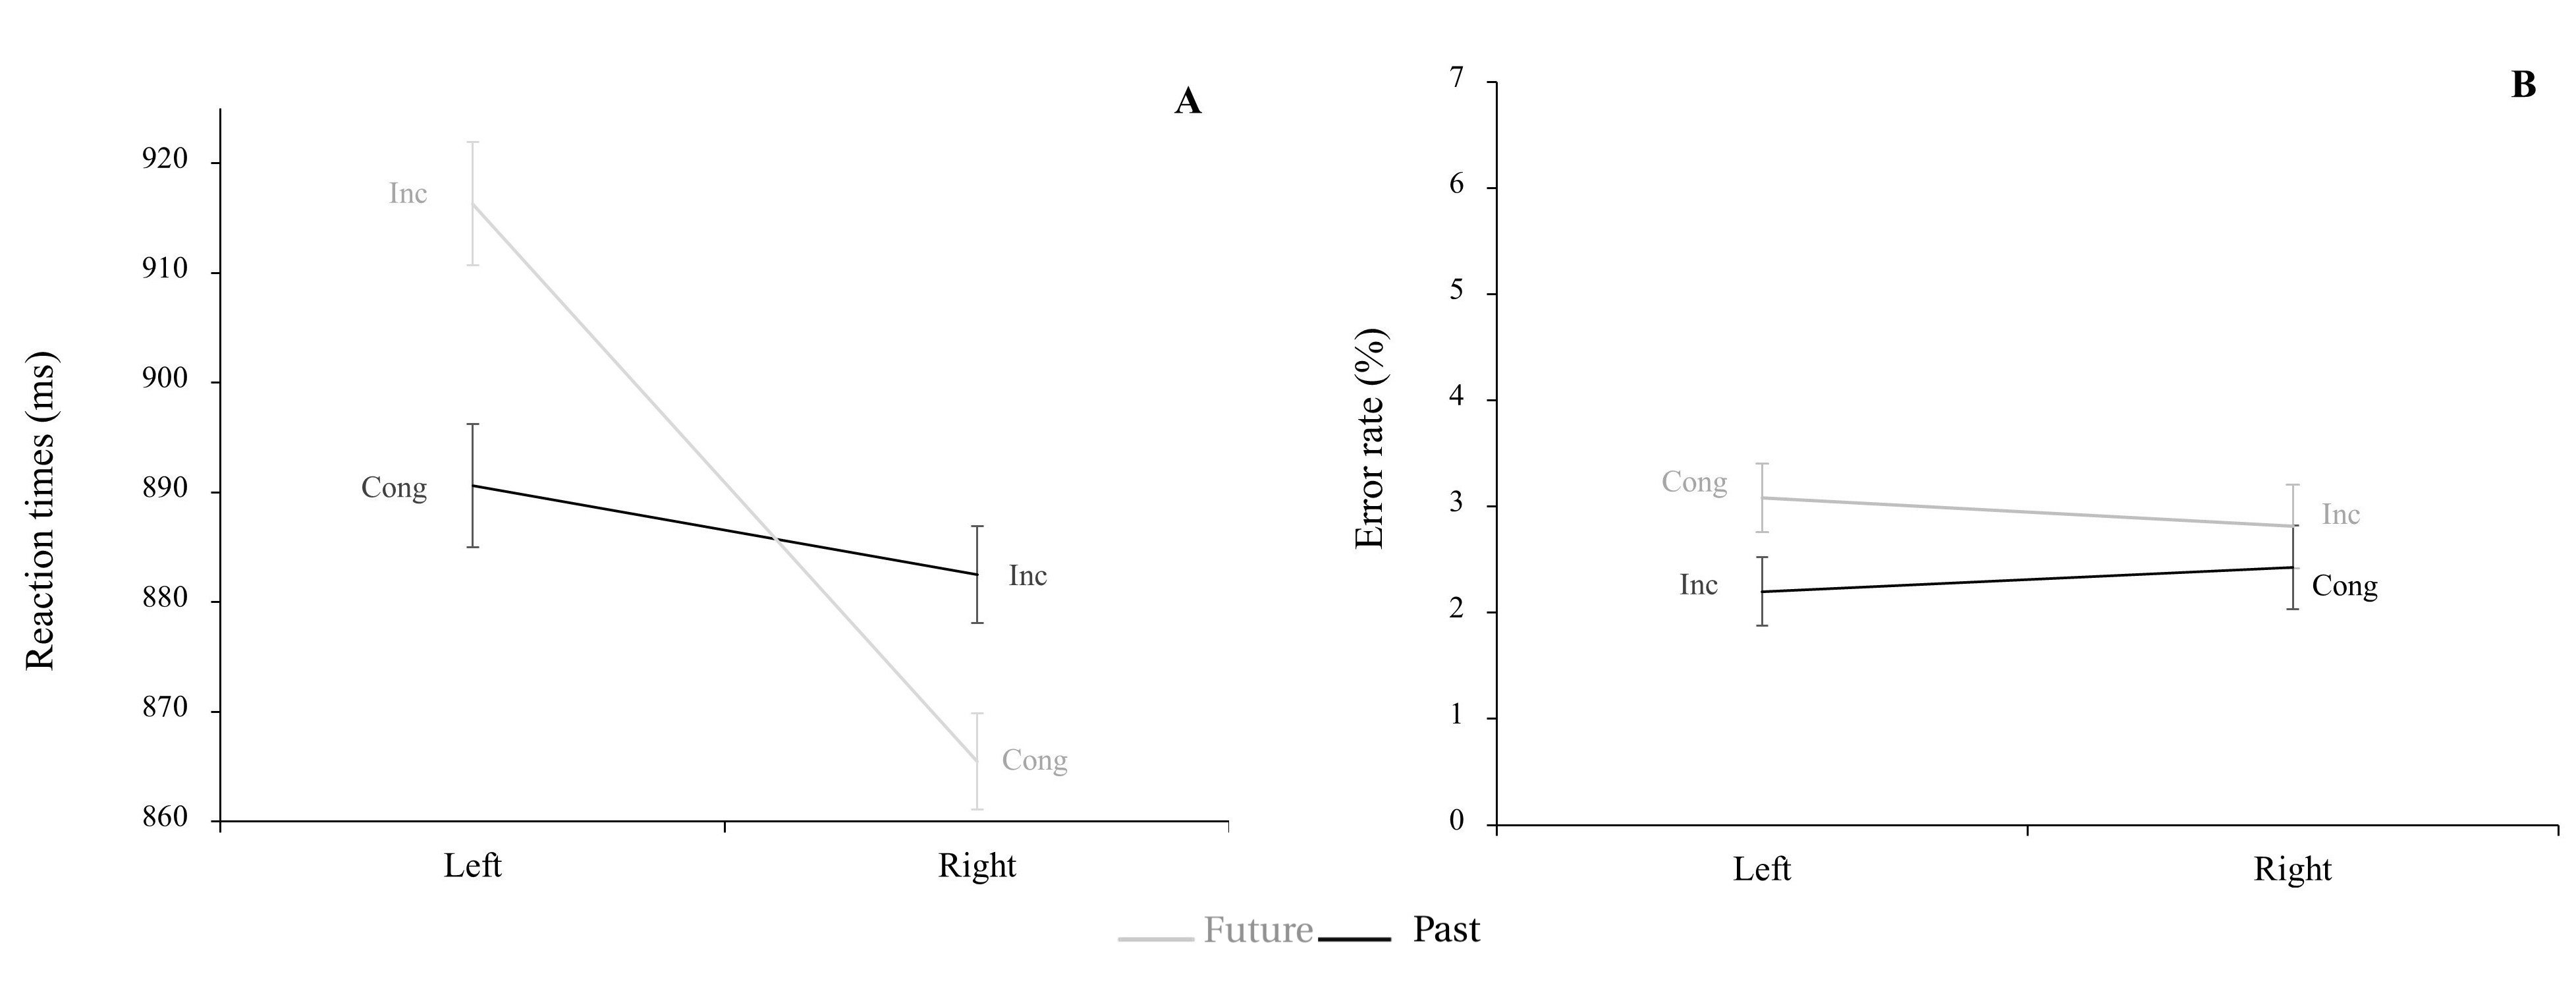
\includegraphics[width=1\linewidth]{figures/chap-3-fig5} 

}

\caption{Experiment 3: Mean Reaction Times (A) and Mean Error Rates (B) as a Function of Response Side (Left Versus Right) and Verb Tense (Past Versus Future). Note : Inc = incongruent, Cong = congruent. Error bars indicate within-participant standard errors.}\label{fig:chap-3-fig5}
\end{figure}

\hypertarget{pseudowords-2}{%
\paragraph{Pseudowords}\label{pseudowords-2}}

The 2 * 2 ANOVA with Side and Time as factors showed no significant main effects of Side or Time and no significant interaction (all \emph{Fs} \textless{} 1). The mixed effects analyses showed no significant effect.

\hypertarget{discussion-2}{%
\subsubsection{Discussion}\label{discussion-2}}

Experiment 3 was designed to rule out the hypothesis that the presentation of a temporal prime prior to the target words might have artificially produced a congruency effect by increasing the temporal salience of the stimuli and/or the task setting. To this end, we replicated the movement condition of Experiment 2, but in the absence of a temporal prime. According to von Sobbe et al.'s classification (\protect\hyperlink{ref-von_sobbe_space-time_2019}{von Sobbe et al., 2019}), this corresponds to an experimental situation in which time is task-irrelevant. As in Experiments 1 and 2, the results of Experiment 3 clearly showed a space-time congruency effect on latencies. These results suggest that the primes used in experiments 1 et 2 were not at the origin of the space-time congruency effect, and provide strong evidence in support of the hypothesis that the left-right mental time-line can be automatically activated in a time-irrelevant task.

\hypertarget{general-discussion}{%
\subsection{General discussion}\label{general-discussion}}

Three experiments were designed to investigate whether the processing of isolated words that carry information about time (i.e., verb tense) would automatically activate spatial and motor networks and consequently affect both word processing and action execution along the left-right axis. To this end, participants performed a lexical decision task on conjugated (past/future) verbs and pseudoverbs by either moving their arm to the left or the right, or by pressing the left or right key of a keyboard. Importantly, the processing of grammatical time was not explicitly required to perform the task and was totally irrelevant for making correct lexical decisions. If words that carry grammatical information about time automatically activate the left/right mental timeline, we expected to observe a detrimental effect for incongruent space-time mappings (i.e., past on the right, future on the left) on both reaction times and error rates. Our results confirm these predictions and further show that directed movement through space was a necessary condition for the occurrence of a congruency effect on response latencies. Our results suggest that previous studies might have failed to find a congruency effect (e.g., \protect\hyperlink{ref-maienborn_we_2015}{Maienborn et al., 2015}; \protect\hyperlink{ref-ulrich_leftright_2010}{Ulrich \& Maienborn, 2010}) because they used static responses, such as key-presses. The three experiments of the present study converge to suggest that movement might be the key component underlying the activation of the mental timeline during semantic processes of grammatical time (past/future).

An interesting question is why words that carry information about time are associated with movement along a left-to-right mental timeline? One possibility might be related to our reading and writing system. Indeed, several behavioral studies have shown that the spatial organization of the mental timeline follows the direction of the reading and writing systems. For example, \protect\hyperlink{ref-fuhrman_mental_2007}{Fuhrman \& Boroditsky} (\protect\hyperlink{ref-fuhrman_mental_2007}{2007}) showed that English speakers (who read and write from left to right) organized temporal events from left to right whereas Hebrew speakers (who read and write from right to left) showed the opposite pattern. This was also observed for Mandarin speakers who read and organize time vertically, with past events above and future events below (\protect\hyperlink{ref-boroditsky_english_2011}{Boroditsky et al., 2011}). Interestingly, a few minutes of mirror reading are sufficient to reverse the direction of the mental timeline (\protect\hyperlink{ref-hutchison_can_2010}{Casasanto \& Bottini, 2010}). According to the authors, this demonstrates the causal role of the directionality of our writing system in the spatial mapping of time along a mental timeline. They concluded that the mental timeline follows writing direction because ``progress through time corresponds to change in position along a linear spatial path'' (\protect\hyperlink{ref-casasanto_spatial_2014}{Casasanto \& Bottini, 2014, p. 6}). It is possible that the direction of the mental timeline emerges from this accumulation of motor experience, with earlier events being ``located'' to the left and later events to the right. This implies that the very representation of a time word (like future- and past-tense verbs) might include the motor execution component of left-to-right movements. Said differently, time words might be spatially embodied as their processing recruits neural networks necessary for motor execution. This would explain why movement seems to constitute a key factor in the automatic activation of the mental timeline.

More generally, the central role of movement in the conceptualization of time is supported by numerous theorical and empirical arguments. For example, in six experiments, \protect\hyperlink{ref-boroditsky_roles_2002}{Boroditsky \& Ramscar} (\protect\hyperlink{ref-boroditsky_roles_2002}{2002}) noted that asking participants to imagine time moving towards them or, alternatively, themselves moving forward in time induced a change in their perspective about past and future events. These results imply that the mental timeline involves not only notions of spatial location but also movement \emph{through} space. Moreover, this relation between motor action and the mental timeline is reflected by spontaneous gestures during speech. Analyses of participants' movements when they are talking about past or future events showed that speakers produced movements directed to the left for past events and to the right for future events (\protect\hyperlink{ref-casasanto_hands_2012}{Casasanto \& Jasmin, 2012}). Indeed, ATOM theory emphasizes that time and space share common mechanisms and brain networks with the motor system because spatial and temporal features are processed simultaneously for every action. \protect\hyperlink{ref-sell_processing_2011}{Sell \& Kaschak} (\protect\hyperlink{ref-sell_processing_2011}{2011}) suggested that the observed space-time congruency effect was the result of activation of intraparietal and parietal regions implicated in the understanding of space, time, quantity and other magnitudes. Interestingly, the same regions are also involved in motor planning. According to the authors, ``the mechanisms that are responsible for preparing and executing bodily action play a role in grounding the comprehension of language about abstract situation'' (\protect\hyperlink{ref-sell_processing_2011}{Sell \& Kaschak, 2011, p. 4}). To our view, movement might be the bodily and physical experience that brings together space and time.

One last issue that should be discussed concerns the automatic activation of the mental timeline and the necessary experimental conditions for a space-time congruency effect to be observed. As discussed in the Introduction, this issue has recently been addressed by \protect\hyperlink{ref-von_sobbe_space-time_2019}{von Sobbe et al.} (\protect\hyperlink{ref-von_sobbe_space-time_2019}{2019}) in a meta-analysis of the results of 30 published studies, in which they observed that the size of the time-space congruency effect was larger in experiments for which time was relevant (\emph{d} = 0.46) or that included temporal priming, (\emph{d} = 0.47) than for experiments in which time was task-irrelevant (\emph{d} = 0.09). This led the authors to conclude that the mental timeline is more likely activated when temporal reasoning is required in the task. For the sake of comparison, we calculated Cohen's d for the space-time congruency effects we observed in Experiments 1 to 3. These results are shown in Figure \ref{fig:chap-3-fig6}. We obtained values ranging from 0.38 to 0.74 (mean 0.45) when the participants answered using movement devices (trackpad and mouse) and 0.15 when participants answered using the keyboard. Note that in all of our experiments time was task-irrelevant (classic lexical decision) and the space-time congruency effect was observed in the absence of temporal priming (Exp 3). Thus, our experiments clearly fall into von Sobbe et al.'s ``time is task-irrelevant'' category, yet our effect sizes are closer to those obtained for experiments in their ``time is relevant'' or ``temporal priming'' categories. One explanation for this has already been discussed (i.e., the importance of movement). The other might have to do with the complexity of the tasks and stimuli used in previous studies. Indeed, in many previous studies, the authors used high-level tasks (sensibility judgments) and more complex stimuli (whole sentences or even stories). If the time-space congruency effect is rather low-level (early and automatic activation of a mental time-line that interferes with basic word recognition processes), one might expect that such effects are more difficult to bring out in more complex or higher-level tasks. Finally, \protect\hyperlink{ref-von_sobbe_space-time_2019}{von Sobbe et al.} (\protect\hyperlink{ref-von_sobbe_space-time_2019}{2019}) made the distinction between \emph{low} and \emph{high} temporal complexity of the task and argued that the activation of the mental timeline (characterized by a significant congruency effect) occurs only when the level of temporal complexity was high. However, this cannot explain why we find comparable effect sizes in our own ``time is task-irrelevant'' experiments to those of von Sobbe et al.'s ``time-is-relevant'' experiments because the temporal complexity of our stimuli was rather low.

\begin{landscape}

\begin{figure}[htbp!]

{\centering 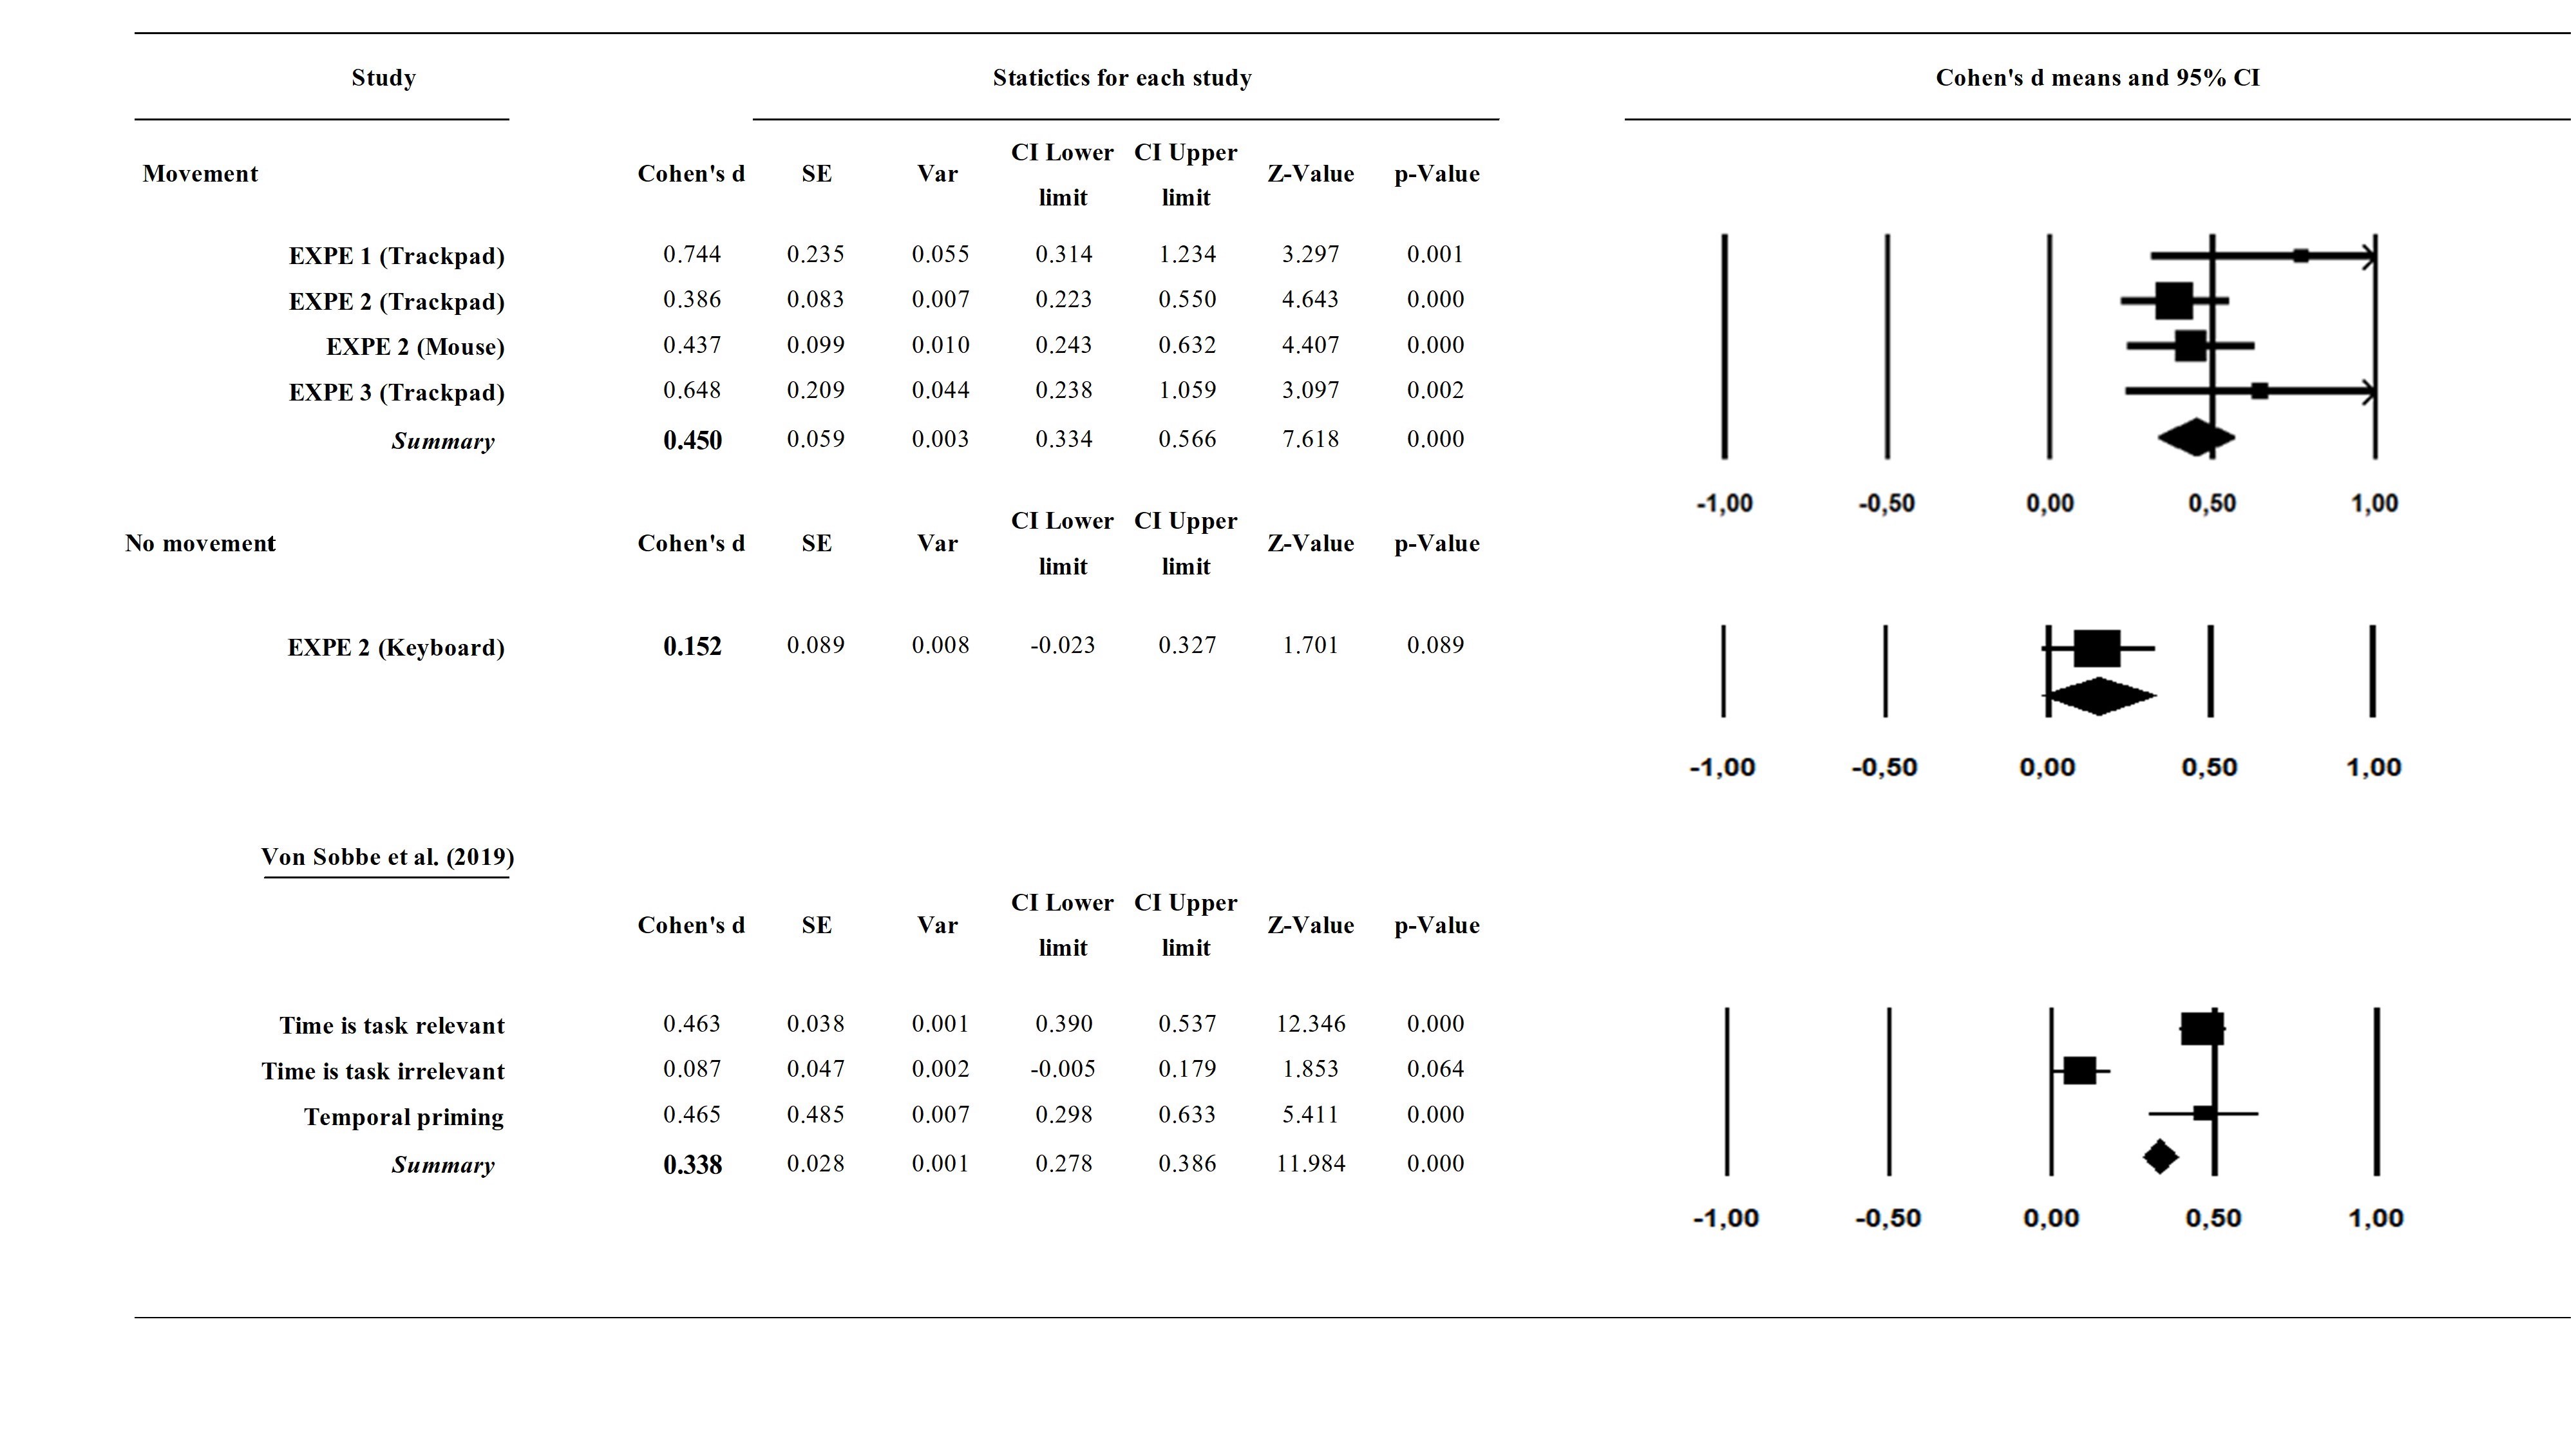
\includegraphics[width=1\linewidth]{figures/chap-3-fig6} 

}

\caption{Summary of the Adjusted Mean Effect Sizes (Cohen’s d) and Corresponding Forest Plot for Our Own Experiments (Upper Panel) and the Results of the Meta-Analysis by von Sobbe et al. (2019) (Lower Panel). Note: SE = standard error; Var = variance; CI = confidence interval.}\label{fig:chap-3-fig6}
\end{figure}

\end{landscape}

To conclude, our results are relevant to a more general debate about how abstract concepts can be embodied. Indeed, according to the embodied view of language, meaning is supported by sensorimotor, introspective and emotional networks (\protect\hyperlink{ref-barsalou_perceptual_1999}{Barsalou, 1999}; \protect\hyperlink{ref-glenberg_revolution_2013}{Glenberg et al., 2013}) with abstract concepts being ``grounded'' like concrete concepts, through experiential interactions during the acquisition of a concept or a meaning. For example, the emotional content of words selectively activates the corresponding primary emotion networks rapidly and automatically (\protect\hyperlink{ref-ponz_emotion_2014}{Ponz et al., 2014}; \protect\hyperlink{ref-ziegler_words_2018}{Ziegler et al., 2018}). Similarly, processing motor and visual abstract words elicits activation in the respective motor and visual brain regions (\protect\hyperlink{ref-kiefer_varieties_2020}{Kiefer \& Harpaintner, 2020}). As suggested by \protect\hyperlink{ref-barsalou_language_2008}{Barsalou et al.} (\protect\hyperlink{ref-barsalou_language_2008}{2008}), ``because concepts emerge from processing situations, they are best studied in the context of situations''(\protect\hyperlink{ref-barsalou_moving_2018}{Barsalou et al., 2018, p. 9}), in which case the dissociation between concrete and abstract concepts appear no longer relevant. In our study, as suggested previously, we most likely found a space-time congruency effect during a non-temporal language task because we studied the abstract concept of time in its situational context, that of movement.

\hypertarget{suppCh3}{%
\section{Supplementary materials}\label{suppCh3}}

Open data, supplementary materials, as well as reproducible code are available at \url{https://osf.io/7gt9k}.

\hypertarget{acknowledgements}{%
\section{Acknowledgements}\label{acknowledgements}}

Camille Grasso was supported by a doctoral fellowship of the French Ministry of Higher Education, Research, and Innovation. This study benefited from support of the Institute of Convergence ILCB (ANR-16-CONV-0002) and the Excellence Initiative of Aix-Marseille University A*MIDEX (ANR-11-IDEX-0001-02).

\newpage

\begin{vplace}[1]

\begin{summary}{Résumé du Chapitre\getcurrentref{chapter}}{\chaptercolor}

Quel est le rôle des structures corticales sensorimotrices pour la représentation de mots désignant des concepts abstraits temporels ? Sur ce point, il a été proposé que les concepts d’ordre temporels seraient conceptualisés spatialement le long d’une ligne mentale temporelle où les évènements passés sont localisés à gauche et les évènements futurs à droite. Si les mots désignant des concepts de passés et de futurs activent automatiquement des structures corticales motrices et spatiales, alors le traitement de ces derniers devrait interférer avec les mouvements de la main qui vont dans la direction opposée. Pour tester l’hypothèse d’une implication automatique, trois tâches de décision lexicale (tâche temporelle implicite et peu complexe) ont été menées. Pour tester le rôle du mouvement, les participant·e·s devaient décider si des verbes et pseudo-verbes conjugués (passé/futur) existaient, soit en répondant en exécutant des mouvements dynamiques (i.e., spatialement dirigés à gauche ou à droite) soit en réalisant des mouvements statiques (i.e., pression d'une touche au clavier). Les résultats de ces trois expériences ont montré des effets de congruence spatio-temporelle uniquement pour les mots existants et uniquement dans les conditions de mouvements dynamiques. Dans l'ensemble, les résultats corroborent l'hypothèse d'une implication automatique d'informations motrices, en plus des informations spatiales gauche-droite, pendant la reconnaissance des mots. Cette observation étaye l’hypothèse d’un ancrage des concepts abstraits temporels lors du mouvement dynamique (i.e., spatialement dirigé). Nous avons suggéré que l’utilisation de réponses motrices statiques lors de tâches temporelles implicites (par exemple, Maienborn et al., 2015; Ulrich \& Maienborn, 2011) pourrait expliquer l’absence d’effet de congruence spatio-temporelle mesurables. La question reste de savoir pourquoi les mots qui désignent des concepts abstraits temporels sont liés à des informations spatiales gauche-droite. Sur ce point, nous avons discuté du rôle de l’expérience sensorimotrice vécue lors de la lecture et de l’écriture. Si les concepts abstraits temporels prennent racine dans un ensemble de mouvements répétés de la gauche vers la droite, comme pendant l’écriture, alors des effets de congruence spatio-temporelle devraient également s’observer lors de mouvements dynamiques effectués avec un autre effecteur, ici les yeux (également impliqués lors de la lecture). La prochaine étude avait deux objectifs principaux : i) étudier si l’effet de congruence spatio-temporelle est centré sur l’effecteur de la main où s’il généralise à un autre effecteur : les yeux, et ii) étudier si le cadre de référence spatiale rattaché aux concepts abstraits temporels est relatif aux effecteurs de la main, ou serait plutôt relatif au corps entier. 

\end{summary}

\end{vplace}

\changechaptercolor{hokusai4}

\hypertarget{chap4}{%
\chapter{Eye movements through space interfere with visual processing of time-related words}\label{chap4}}

\initial{W}hen people make lexical decisions to words referring to the past or the future, they are faster when their manual responses are compatible with the mental timeline (MTL). That is, future words are responded to faster on the right than the left, while past words are responded to faster on the left than the right. This space-time congruency effect is interpreted to suggest that time words are represented along a spatial continuum that goes from left to right (past to future), at least in Western cultures that use reading-writing systems operating from left to right. All previous experiments used lateralized hand movements to register responses, which would evoke the directionality of writing. To evoke the directionality of reading, we investigated whether the space-time congruency effect would be replicated in a language task when responses were given using the eyes rather than the hand. Thus, participants were asked to make lateralized eye movements to indicate whether letter stimuli were real words or not (lexical decision). Eye movements were perturbed for responses incompatible with the direction of the MTL, both in terms of decision time and motor amplitude. These results confirm that time-related words are embodied through spatial movement in effector-independent motor networks and suggests that the spatial representation of time operates in a body-centered reference frame.\footnote{Ce chapitre expérimental est une version adaptée du manuscrit au format de la thèse. Pour trouver le préprint de la version soumise au journal Acta Psychologica: Les stimuli, les scripts, les données et les figures sont disponibles en ligne: \url{https://osf.io/5ehnc/}.}

\hypertarget{introduction-1}{%
\section{Introduction}\label{introduction-1}}

One of the big challenges for theories of embodied language has been to show how they can handle the representation of abstracts words that do not directly refer to any physical object (e.g., \emph{future}, \emph{freedom}, \emph{quantum physics}), and thus cannot be associated with direct sensorimotor information. Empirical evidence suggests that abstract words can indeed be associated with sensory interoceptive or emotional information (e.g., \protect\hyperlink{ref-connell_interoception_2018}{Connell et al., 2018}; \protect\hyperlink{ref-vigliocco_neural_2014}{Vigliocco et al., 2014}; \protect\hyperlink{ref-villani_sensorimotor_2021}{Villani et al., 2021}). The distinction between abstract and concrete words might not be as important as previously thought (e.g., \protect\hyperlink{ref-barsalou_moving_2018}{Barsalou et al., 2018}; \protect\hyperlink{ref-barsalou_challenges_2020}{Barsalou, 2020}; \protect\hyperlink{ref-kiefer_varieties_2020}{Kiefer \& Harpaintner, 2020}). For example, recent meta-analyses of neuroimaging data have found strong overlapping activations for the processing of concrete and abstracts concepts (e.g., \protect\hyperlink{ref-desai_multifaceted_2018}{Desai et al., 2018}; \protect\hyperlink{ref-harpaintner_grounding_2020}{Harpaintner et al., 2020}).

In the present article, we investigated the type of embodied information that contributes to the representation of words referring to the abstract concept of time. Time is not associated with any tangible temporal stimulus, there are no sensory receptors for time, and no ``time area'' in the brain. So, how do we represent and understand the abstract meaning of time? One of the major theoretical frameworks for the conceptualization of time is the mental timeline (MTL, for reviews, see \protect\hyperlink{ref-bender_mapping_2014}{Bender \& Beller, 2014}; \protect\hyperlink{ref-bonato_when_2012}{Bonato et al., 2012}; \protect\hyperlink{ref-cooperrider_across_2009}{Cooperrider \& Núñez, 2009}). This account claims that time is spatially organized along linear axes, particularly for concepts of temporal order (e.g., past, future). This spatialization of time is culturally dependent (e.g., \protect\hyperlink{ref-bonato_when_2012}{Bonato et al., 2012}; \protect\hyperlink{ref-boroditsky_remembrances_2010}{Boroditsky \& Gaby, 2010}; \protect\hyperlink{ref-nunez_contours_2012}{Núñez et al., 2012}; \protect\hyperlink{ref-oliveri_representation_2009}{Oliveri et al., 2009}). Converging cross-cultural data with distinct writing and reading systems have shown that Western cultures, with a left-to-right writing system, develop a left-past vs.~right-future mental timeline. In cultures with a right-to-left writing system, the MTL is right-to-left (\protect\hyperlink{ref-ouellet_is_2010}{Ouellet, Santiago, Israeli, et al., 2010}). Therefore, it has been suggested that the left-to-right MTL results from extensive left-to-right reading and writing experience in orthographic systems that use that direction (e.g., \protect\hyperlink{ref-fuhrman_mental_2007}{Fuhrman \& Boroditsky, 2007}).

Several studies have shown that words related to the past or the future activate the MTL, which suggests that the semantic representation of time includes spatial information. A way to experimentally show this is to set up a laboratory task, in which participants respond leftwards or rightwards to words that refer to either the past or the future. If linguistic representations of time use space to convey the flow of time from the past to the future (i.e., activate a MTL), then asking participants to respond by moving their hand to the left for future words and to the right for past words creates interference, a space-time incongruency. Indeed, such a space-time congruency effect has been observed in various language tasks (e.g., \protect\hyperlink{ref-eikmeier_response_2015}{Eikmeier, Hoppe, et al., 2015}; \protect\hyperlink{ref-kong_space-time_2012}{Kong \& You, 2012}; \protect\hyperlink{ref-maienborn_we_2015}{Maienborn et al., 2015}; \protect\hyperlink{ref-santiago_time_2007}{Santiago et al., 2007}; \protect\hyperlink{ref-torralbo_flexible_2006}{Torralbo et al., 2006}; \protect\hyperlink{ref-ulrich_leftright_2010}{Ulrich \& Maienborn, 2010}).

In these studies, the space-time congruency effect was strong when participants were asked to make explicit past/future judgments about words or sentences (e.g., \protect\hyperlink{ref-aguirre_potential_2017}{Aguirre \& Santiago, 2017}; \protect\hyperlink{ref-hutchison_can_2010}{Casasanto \& Bottini, 2010}; \protect\hyperlink{ref-de_la_vega_mental_2016}{de la Vega et al., 2016}; \protect\hyperlink{ref-kong_space-time_2012}{Kong \& You, 2012}), but considerably reduced or absent when participants were instead asked to make judgments about a non-temporal dimension, such as word lexicality or semantic congruency (\protect\hyperlink{ref-maienborn_we_2015}{Maienborn et al., 2015}; \protect\hyperlink{ref-von_sobbe_space-time_2019}{von Sobbe et al., 2019}, for a meta-analysis). The reduction of the space-time congruency effect in tasks that do not involve direct and explicit processing of time was taken to suggest that the MTL is not activated automatically (\protect\hyperlink{ref-maienborn_we_2015}{Maienborn et al., 2015}; \protect\hyperlink{ref-von_sobbe_space-time_2019}{von Sobbe et al., 2019}). However, \protect\hyperlink{ref-grasso_as_2021}{Grasso, Ziegler, Mirault, et al.} (\protect\hyperlink{ref-grasso_as_2021}{2021}) have recently demonstrated that one can find such space-time congruency effects in a language task that does not involve the explicit processing of time (i.e., lexical decision) as long as participants gave their response making hand movements (leftward or rightward) though not if they simply pressed a left or a right key (see also \protect\hyperlink{ref-sell_processing_2011}{Sell \& Kaschak, 2011}; replicated by \protect\hyperlink{ref-scheifele_replication_2018}{Scheifele et al., 2018}). This finding suggested that left- or rightward movement through space is a critical aspect for the representation of past or future words.

It is usually admitted that space-time congruency effects are due to the involvement of a single egocentric map where objects, actions and even notions are represented. The centre of this full-body egocentric spatial reference frame corresponds to the median axis of the body (e.g., \protect\hyperlink{ref-fuhrman_cross-cultural_2010}{Fuhrman \& Boroditsky, 2010}; \protect\hyperlink{ref-miles_mapping_2010}{Miles et al., 2010}; for a discussion see for example \protect\hyperlink{ref-nunez_contours_2012}{Núñez et al., 2012}). As an alternative to that unitary framework, space-time congruency effects might be built on multiple reference frames, each being dedicated to a given spatial location and/or a given class of action and/or motor effector (for more information about these different spatial frames, see \protect\hyperlink{ref-ghafouri_contribution_2006}{Ghafouri \& Lestienne, 2006}). In all previous experiments on space-time congruency effects, interference was generated using the hand as the response effector (e.g., \protect\hyperlink{ref-eikmeier_how_2015}{Eikmeier, Alex-Ruf, et al., 2015}; \protect\hyperlink{ref-kong_space-time_2012}{Kong \& You, 2012}; \protect\hyperlink{ref-maienborn_we_2015}{Maienborn et al., 2015}; \protect\hyperlink{ref-santiago_time_2007}{Santiago et al., 2007}; \protect\hyperlink{ref-torralbo_flexible_2006}{Torralbo et al., 2006}; \protect\hyperlink{ref-ulrich_leftright_2010}{Ulrich \& Maienborn, 2010}). Therefore, it might be that the observed space-time congruency effect for words relies on a spatial reference frame specific to the hand and hand-movements. If words referring to time are represented in a full-body-centered reference frame, space-time congruency effects with words should not rely on a particular effector (the hand) but should generalize to different effectors.

In the present study, we investigate the space-time congruency effect in a language task using the eyes as response effectors. Thus, the present study has two goals. First, if the spatial representation of the temporal content of words derives from repeated directional movements produced during writing and reading, then the space-time congruency effect should not be limited to hand movements (used during writing) but should be observed for eye movements (used during reading) as well. Second, given that goal-directed movements require translation of spatial information into motor commands, a replication of the congruency effect with eye movements would mean that the representations of words referring to time are bound to general motor planning circuits that operate in a full-body-centered spatial frame (\protect\hyperlink{ref-rosenbaum_human_1991}{Rosenbaum, 1991}; \protect\hyperlink{ref-schmidt_motor_2019}{Schmidt et al., 2019}).

To this end, we performed a lexical decision experiment where participants responded using eye movements. French verbs and pseudo verbs were presented in conjugated form (i.e., past or future) on a screen, and participants had to decide as quickly as possible whether the stimulus was a word or a pseudoword by producing a saccade towards the left or the right side of the screen. Experimental design and stimuli were taken from \protect\hyperlink{ref-grasso_as_2021}{Grasso, Ziegler, Mirault, et al.} (\protect\hyperlink{ref-grasso_as_2021}{2021}). The grammatical verbal system in French makes it possible to use the same word stem combined with a suffix that indicates either past tense (je marchais {[}I walked{]}; je rêvais {[}I dreamt{]}) or future tense (je marcherai {[}I will walk{]}; je rêverai; {[}I will dream{]}). Having the same word stem for different temporal conditions nicely controls for possible orthographic, lexical, and semantic confounds. Participants performed both congruent and incongruent conditions. In the congruent condition, eye movements were congruent with the MTL (i.e., past tense verbs required a leftward eye movement; future tense verbs a rightward eye movement). In the incongruent condition, eye movements were incongruent with the MTL.

\hypertarget{materials-and-methods}{%
\section{Materials and Methods}\label{materials-and-methods}}

\hypertarget{participants-3}{%
\subsection{Participants}\label{participants-3}}

The study involved 64 participants from Aix-Marseille University (Marseille, France). Nine participants were excluded from the analyses due to high errors rates or technical data acquisition issues. The remaining 58 participants (48 women, 54 right-handed) were all French native speakers, reported normal or corrected-to-normal vision and no neurological or psychiatric disorder. They ranged in age from 18 to 42 years old (\emph{M} = 22.2; \emph{SD} = 4.6) and signed informed-consent forms prior to participation. The study was conducted in accordance with the recommendations of the World Medical Association Declaration of Helsinki and it was approved by the Institutional Review Board of Aix-Marseille University.

\hypertarget{design-and-stimuli-1}{%
\subsection{Design and Stimuli}\label{design-and-stimuli-1}}

Because the main objective of this study was to determine whether we could replicate the space-time congruency effect observed when participants performed directed movement using the eyes as response effector, we used the design of the experiment 1 of \protect\hyperlink{ref-grasso_as_2021}{Grasso, Ziegler, Mirault, et al.} (\protect\hyperlink{ref-grasso_as_2021}{2021}). We voluntarily chose the first experiment because it was the one with the strongest effect size (Cohen's \emph{d} = .74). In experiments 2 and 3 of their study, \protect\hyperlink{ref-grasso_as_2021}{Grasso, Ziegler, Mirault, et al.} (\protect\hyperlink{ref-grasso_as_2021}{2021}) directly tested the role of temporal priming (i.e., whether ``yesterday/tomorrow'' preceded the conjugated verb) and found no influence of the prime on the space-time congruency effect. Stimuli were also taken from \protect\hyperlink{ref-grasso_as_2021}{Grasso, Ziegler, Mirault, et al.} (\protect\hyperlink{ref-grasso_as_2021}{2021}) and consisted of 80 word stimuli (verbs) and 80 pseudoword stimuli (\emph{pseudoverbs}, see Appendix in \protect\hyperlink{ref-grasso_as_2021}{Grasso, Ziegler, Mirault, et al.} (\protect\hyperlink{ref-grasso_as_2021}{2021}). Each word or pseudoword was presented in past- or future-tense (e.g., je laissais/je laisserai and je gontrais/je gontrerai for words and pseudowords respectively), at the centre of the screen (see Figure \ref{fig:chap-4-fig1}). To ensure that participants saw each word and each pseudoword only once, we created four counterbalanced lists of 160 stimuli each (80 words, 80 pseudowords) using a Latin-Square design. Half of the stimuli in each list were in the past tense, half were in the future tense. All stimuli were preceded by the pronoun ``I'' (je).

\hypertarget{apparatus-1}{%
\subsection{Apparatus}\label{apparatus-1}}

Eye movements were recorded with an EyeLink 1000 system (SR Research, Mississauga, ON, Canada) with a high spatial resolution (0.01°) and a sampling rate of 1000 Hz. Viewing was binocular, but only the right eye was monitored. Stimuli were displayed on a 20-inch ViewSonic CRT monitor with a refresh rate of 85Hz and a screen resolution of 1024 x 768 pixels (30 x 40 cm). Stimuli were presented in black 37-point monospaced fonts (droid sans mono) on a grey background. The experiment was created using OpenSesame (Version 3.2.6; Mathôt et al., 2012). Participants were instructed to give a Yes (``it's a word'') or No (``it's not a word'') response in a lexical decision task by moving their eyes towards the right or left of the screen. The left and right correct response areas of the screen were spatially delimited by two virtual boundaries at +/-600 pixels from the centre of the screen. Participants were seated 86 cm from the monitor, such that every 3 characters equalled approximately 1° of visual angle. We used a chin-rest to minimize head movements.

\hypertarget{procedure-1}{%
\subsection{Procedure}\label{procedure-1}}

The experiment was run in a quiet testing room. Participants received instructions both from the experimenter and from short sentences displayed on the screen. They were instructed to decide as rapidly and as accurately as possible whether the stimulus was a real French word or not (i.e., a lexical decision) by moving their eyes towards the left / right side of the screen. Half of the participants started with ``yes'' responses towards the left, half of the participants started with ``yes'' responses towards the right, and all participants switched response sides halfway through the experiment. Participants completed a short training session of 20 trials before the experimental trials began, and another short training session before switching response side. Each participant saw a total of 80 words and 80 pseudowords randomized across two counterbalanced blocks (``yes'' to the right or ``yes'' to the left). When the ``yes'' response was to the right, future-tense words (20 stimuli) were congruent and past-tense words (20 stimuli) were incongruent (see Figure \ref{fig:chap-4-fig1}). When the ``yes'' response was to the left, past-tense words were congruent (20 stimuli) and future-tense words were incongruent (20 stimuli). In each block, we therefore had 20 words per condition giving a total of 40 words, in addition to 40 future-tense and past-tense pseudowords. This design allowed us to present each stimulus in the past or future tense, during the first or the second part of the experiment, and in the congruent or incongruent condition. At the beginning of the experiment, the position of the eyes was calibrated using a 9-point calibration grid. The experiment started once the training session was completed. Each trial started with a drift correction dot presented at the centre of the screen. Participants were instructed to fixate this dot. Their fixation triggered the onset of a prime stimulus: (``hier'' or ``demain''; ``yesterday'' or ``tomorrow'' in English) that was displayed for 500ms, followed by a 400ms blank screen and then finally by the stimulus (i.e., a word or pseudoword). The stimulus remained on the screen until the participants responded by making a saccade. Saccades that crossed the virtual left or right boundaries were considered as responses, whereas saccades that did not cross the boundaries were considered as refixations or microsaccades (depending on their amplitude). Saccade response side was automatically registered when the eyes crossed the left or right boundary. Responses times corresponded to saccade latency, that is the time between the onset of the stimulus and the onset of the saccade. To assess the kinematic features of the saccade, we measured saccade amplitude expressed in degrees of visual angle (DVA). After each response, participants were instructed to fixate the central black dot to start the next trial. Therefore, a new trial did not start unless the gaze was at the centre of the screen. In each trial, the time interval between the onset of the stimulus and the new fixation dot was set to 2500ms. A break was offered to the participants every 20 trials. Half-way through the experiment (80 trials) participants were instructed to switch sides for yes/no responses. They were trained with the new response sides for 20 trials before completing the second half of the experiment. In all, each session with one participant lasted approximately 1 hour.

\begin{figure}[htbp!]

{\centering 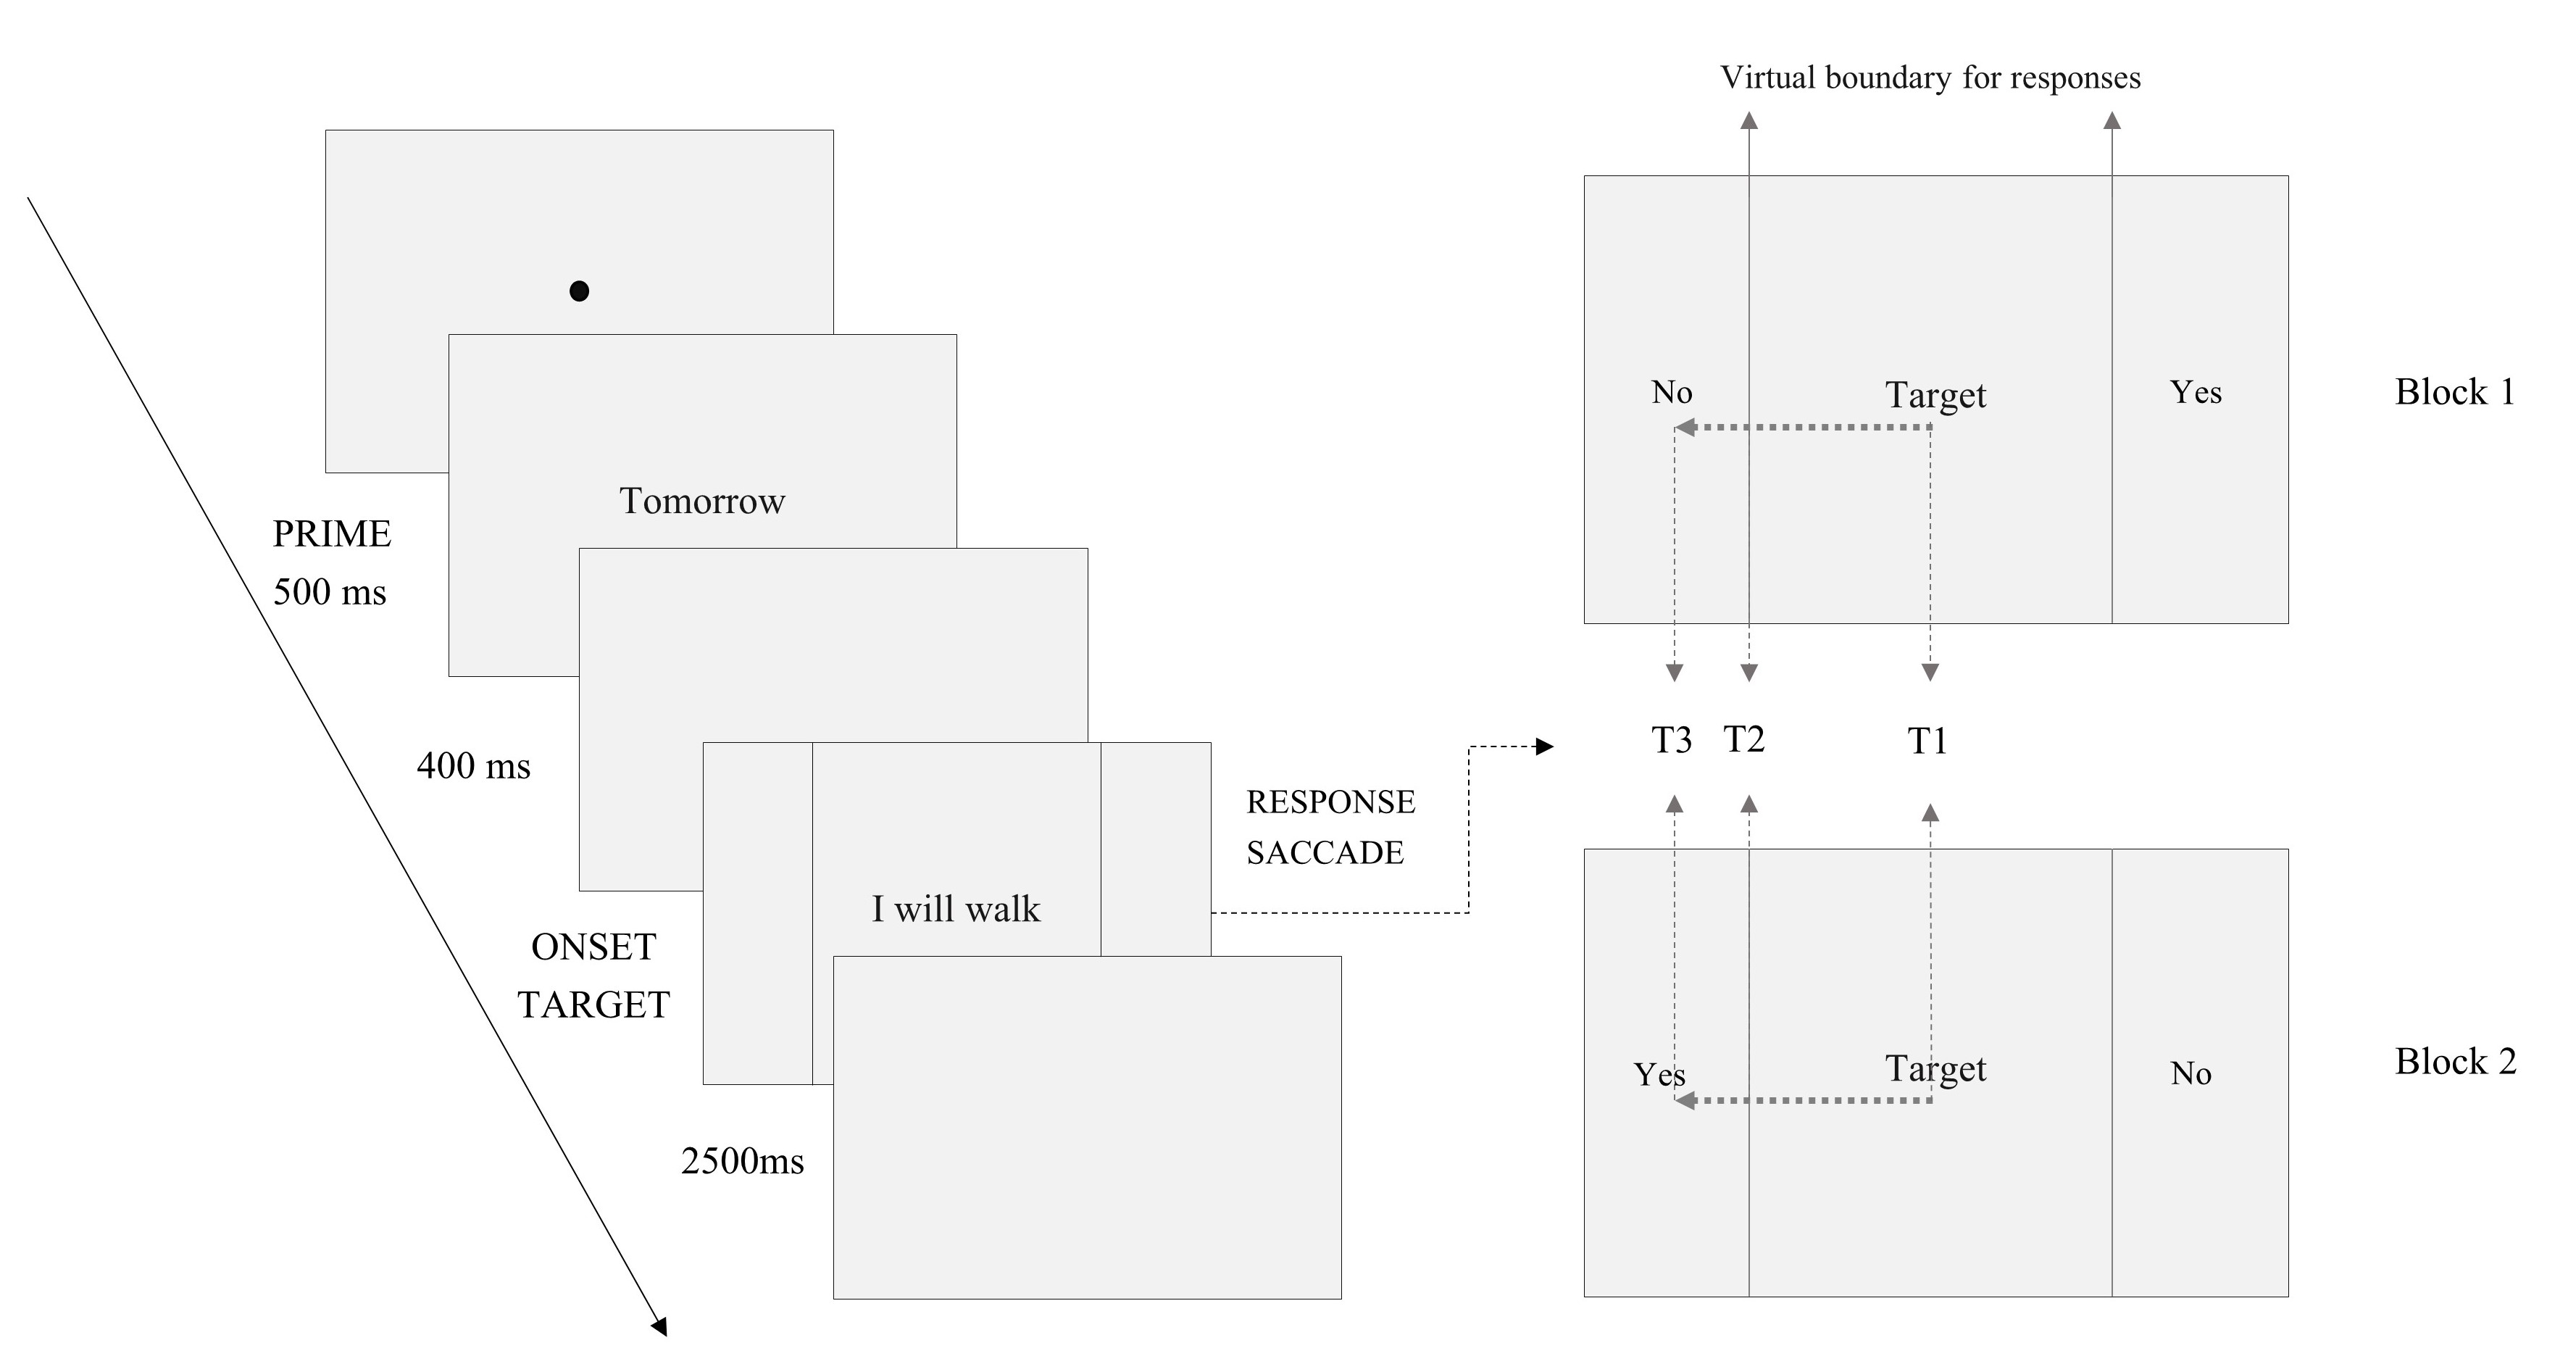
\includegraphics[width=1\linewidth]{figures/chap-4-fig1} 

}

\caption{Task design. After the fixation dot, a prime (“yesterday” or “tomorrow”) was displayed, followed by the word or pseudoword. Participants made their lexical decision by moving their eyes towards the left or right side of the screen. The stimulus disappeared as soon as the eyes moved away from the stimulus. To start a new trial, participants had to fixate the central dot. In this example, the yes-response for the word conjugated in the future tense is congruent in Block 1 (rightward eye movement) but incongruent in Block 2 (leftward eye movement). A saccade was considered to be correct when it reached the left or right virtual boundaries. T1 corresponds to the onset-time of the saccade, T2 corresponds to the boundary-crossing time, and T3 corresponds to the landing time. Therefore, response latencies correspond to the response initiation time, which is the delay between the onset of the stimulus and onset of the saccade.}\label{fig:chap-4-fig1}
\end{figure}

\hypertarget{data-analyses-1}{%
\subsection{Data analyses}\label{data-analyses-1}}

We recorded and analyzed response latency (in milliseconds), and saccade amplitude (in degrees of visual angle). Saccadic eye movements are stereotyped ballistic movements, that is, they cannot be modified once initiated (\protect\hyperlink{ref-gilchrist_saccades_2011}{Gilchrist, 2011}), and they can be described by their latency and their angular rotation (\protect\hyperlink{ref-findlay_visual_2001}{Findlay \& Gilchrist, 2001}; i.e., spatial amplitude of the saccade, \protect\hyperlink{ref-findlay_active_2003}{Findlay \& Gilchrist, 2003}). Saccade latency corresponds to the time needed to process the visual stimulus, to make a decision, and to program the motor response (\protect\hyperlink{ref-gilchrist_saccades_2011}{Gilchrist, 2011}). Saccade amplitude corresponds to the spatial distance between starting and landing positions of the eyes. Although this feature of the saccade may appear to be stereotyped (\protect\hyperlink{ref-edelman_influence_2007}{Edelman et al., 2007}; \protect\hyperlink{ref-findlay_model_1999}{Findlay \& Walker, 1999}), it has been shown that linguistic factors (e.g., unusual orthographic patterns) influence saccade amplitude (\protect\hyperlink{ref-beauvillain_center_1996}{Beauvillain et al., 1996}). Given that the accuracy of goal-directed movements, including saccades, ``depends on the quality of the encoding of spatial information by the central nervous system and the frame of reference'' (\protect\hyperlink{ref-ghafouri_contribution_2006}{Ghafouri \& Lestienne, 2006}), we predicted that saccade programming as measured by saccade amplitude should be sensitive to the space-time frequency effect. Obtaining such an effect would imply that motor planning networks are involved in the spatial representation of words referring to time.

Both saccade latency and amplitude were analyzed using linear Mixed Effect Models (LMEs) with participants and items as crossed random effects (\protect\hyperlink{ref-baayen_analyzing_2008}{Baayen, 2008}; \protect\hyperlink{ref-barr_random_2013}{Barr, 2013}). Note that the space-time congruency effect is indexed by the interaction between the interaction between response side and verb tense. That is, when the side of response for a past-tense word (e.g., I walked) switches from left to right from one block to the other, the word stops being congruent and, instead, becomes incongruent. Similarly, when the side of the response for a future-tense word (e.g., I will walk) switches from left to right, the word stops being incongruent and becomes congruent (see Figure \ref{fig:chap-4-fig1}). Data were fitted with lmer functions from the \texttt{lme4} package (\protect\hyperlink{ref-R-lme4}{Bates et al., 2018}) in the \texttt{R} statistical computing environment (Version 3.5.2, \protect\hyperlink{ref-r_core_team_r_2020}{R Core Team, 2020}). We report unstandardized regression coefficients, standard errors (SEs), and t values. Fixed effects were deemed reliable if \textbar t\textbar{} was greater than 1.96 (\protect\hyperlink{ref-baayen_mixed-effects_2008}{Baayen et al., 2008}). As concerns model building, we used the maximal random structure model that reached convergence (\protect\hyperlink{ref-barr_random_2013}{Barr, 2013}), and this included by-participant and by-item random intercepts in all analyses that we report. In a forward stepwise model selection procedure, fixed and random effects of the models were selected according to the Akaike Information Criterion (AIC, \protect\hyperlink{ref-akaike_maximum_1973}{Akaike, 1973}), the Bayesian Information Criterion (BIC, \protect\hyperlink{ref-schwarz_estimating_1978}{Schwarz, 1978}) using the \texttt{anova()} function of the package \texttt{lmerTest} package (\protect\hyperlink{ref-R-lmerTest}{Kuznetsova et al., 2018}) for model comparison. Therefore, fixed effects, random effects, and random slopes were only included if they significantly improved the model's fit. Assumptions application were checked for each model: residual distribution were checked visually by plotting the residuals' \texttt{Quantile-Quantile} (QQ) and the normality of the distribution of the random effects by plotting the QQ-plots with the \texttt{qqmath()} function (\protect\hyperlink{ref-sarkar_lattice_2008}{Sarkar, 2008}) and the \texttt{ranef()} function. Following the procedure described by \protect\hyperlink{ref-brysbaert_power_2018}{Brysbaert \& Stevens} (\protect\hyperlink{ref-brysbaert_power_2018}{2018}), we conducted power analysis based on 200 simulations with \texttt{powerSim} functions from the \texttt{simR} package (\protect\hyperlink{ref-green_simr_2016}{Green \& MacLeod, 2016}). To create the figures, we used the \texttt{emmeans} package (\protect\hyperlink{ref-lenth_emmeans_2021}{Lenth, 2021}) that allows us to compute the estimated marginals means (EMMs) for the interaction between response side and verb tense for each model (see Figure \ref{fig:chap-4-fig2} and Figure \ref{fig:chap-4-fig3}).

\hypertarget{results-3}{%
\section{Results}\label{results-3}}

Saccade latency and saccade amplitude were analysed for the 58 participants. First, we removed trials containing blinks (2.91\%), no-response trials (2.21\%), trials with negative fixation duration (i.e., below 0ms, 2.41\%), trials in which the initial position of the response saccade on the x-axis was outside the left or right boundaries (0.72\%) and trials with a total fixation duration below 100ms (anticipatory responses, 1.63\%). We further discarded aberrant values corresponding to trials with latencies greater than the possible trial duration (i.e., above 2500ms) or less than 300ms (0.06\% of trials in total), and trials with saccade amplitude greater than 30 degrees and less than 2 degrees (0.20\%). Finally, after removing trials in which the participant gave an incorrect response (3.91\%) latency outliers were removed following the classic ± 2.5 standard deviations from the participants' mean response time (2.66\% of the trials). Statistical analyses were conducted separately for words and pseudowords.

\hypertarget{words-3}{%
\subsection{Words}\label{words-3}}

For the analysis of saccade latencies, the final model included the following fixed effects: Time (past vs future), Side (left vs right) and their interaction, as well as word length (in pixels) and the number of word refixations (i.e., the number of fixations that were made on the word before answering) as covariates. The model also included by-participant and by-item random intercepts, and a random slope for Time, Side and number of refixations by-participants and a random slope for time by-items.

Overall, participants were significantly faster to initiate a response saccade to the right side of the screen than to the left side (\emph{b} = 20.63, \emph{SE} = 10.14, \emph{t} = 2.03, \emph{p}\textless{} .05) but there was no significant difference for past versus future tense words (\emph{b} = 11.86, \emph{SE} = 8.62, \emph{t} = 1.37, \emph{p}= .17). Unsurprisingly, saccade latencies increased significantly with word length (\emph{b} = 1.10, \emph{SE} = 0.27, \emph{t} = 4.30, \emph{p}\textless{} .0001) and number of refixations (\emph{b} = 84.97, \emph{SE} = 5.83, \emph{t} = 14.57, \emph{p}\textless{} .0001). Importantly, the congruency effect, which is the interaction between Time and Side, was highly significant (\emph{b} = -26.49, \emph{SE} = 9.90, \emph{t} = 2.68, \emph{p}=.007). That is, saccade latencies to past-tense stimuli were slower when the correct (``yes'') response was on the right rather than the left. And saccade latencies for future-tense verbs were slower when the correct response was on the left versus the right (see Figure \ref{fig:chap-4-fig2}). The power of this model (i.e., congruency and time) in 200 simulated studies was .81, 95\%CI = {[}74, 86{]}. No other effect or interaction was significant.

The final model for the analysis of saccade amplitude included Time (past vs future), Side (left vs right) and their interaction as fixed effects, as well as number of refixations as a covariate. The model also included by-participant and by-item random intercepts, and a random slope for Side by-participant. Results showed a marginal effect of the number of word refixations (\emph{b} = -0.05, \emph{SE} = 0.02, \emph{t} = 1.89, \emph{p}=.06). More importantly, the interaction between Time and Side was significant (\emph{b} = -0.20, \emph{SE} = 0.08, \emph{t} = 2.28, \emph{p} =.02) reflecting the space-time congruency effect (see Figure \ref{fig:chap-4-fig3}). The power of this model (i.e., congruency and time) in 1000 simulated studies was .66, 95\% CI = {[}59, 73{]}. No other effect or interaction was significant.

\hypertarget{pseudowords-3}{%
\subsection{Pseudowords}\label{pseudowords-3}}

For the analysis of saccade latencies, the final model included Time (past vs future), Side (left vs right) and their interaction as fixed effects, as well as word length (in pixels) and number of refixations as covariates. The model also included by-participant and by-item random intercepts, and a random slope for Time, Side, and number of refixations by-participants and a random slope for Time by-items. Saccade latencies increased significantly as a function of pseudoword length (\emph{b} = 0.81, \emph{SE} = 0.26, \emph{t} = 3.19, \emph{p} \textless{} .001) and the number of refixations (\emph{b} = 83.60, \emph{SE} = 5.41, \emph{t} = 15.45, \emph{p} \textless{} .0001). The interaction between Time and Side was not significant (\emph{b} = 3.17, \emph{SE} = 9.74, \emph{t} = 0.33, \emph{p} = .74). No other effect or interaction was significant.

The final model for the analysis of saccade amplitude included Time (past vs future), Side (left vs right), number of pseudoword refixations and their interaction as fixed effects, and by-participant and by-item random intercepts. Results showed a significant effect of Side (\emph{b} = 0.00, \emph{SE} = 0.00, \emph{t} = 3.05, \emph{p} \textless{} .01), number of pseudoword refixations (\emph{b} = 0.00, \emph{SE} = 0.00, \emph{t} = 4.35, \emph{p} \textless{} .001) and a signification interaction between them (\emph{b} = 0.00, \emph{SE} = 0.00, \emph{t} = 5.92, \emph{p} \textless.001), that is, participants made more refixations before responding to the left than to the right. No other effect or interaction was significant.

\begin{figure}[htbp!]

{\centering 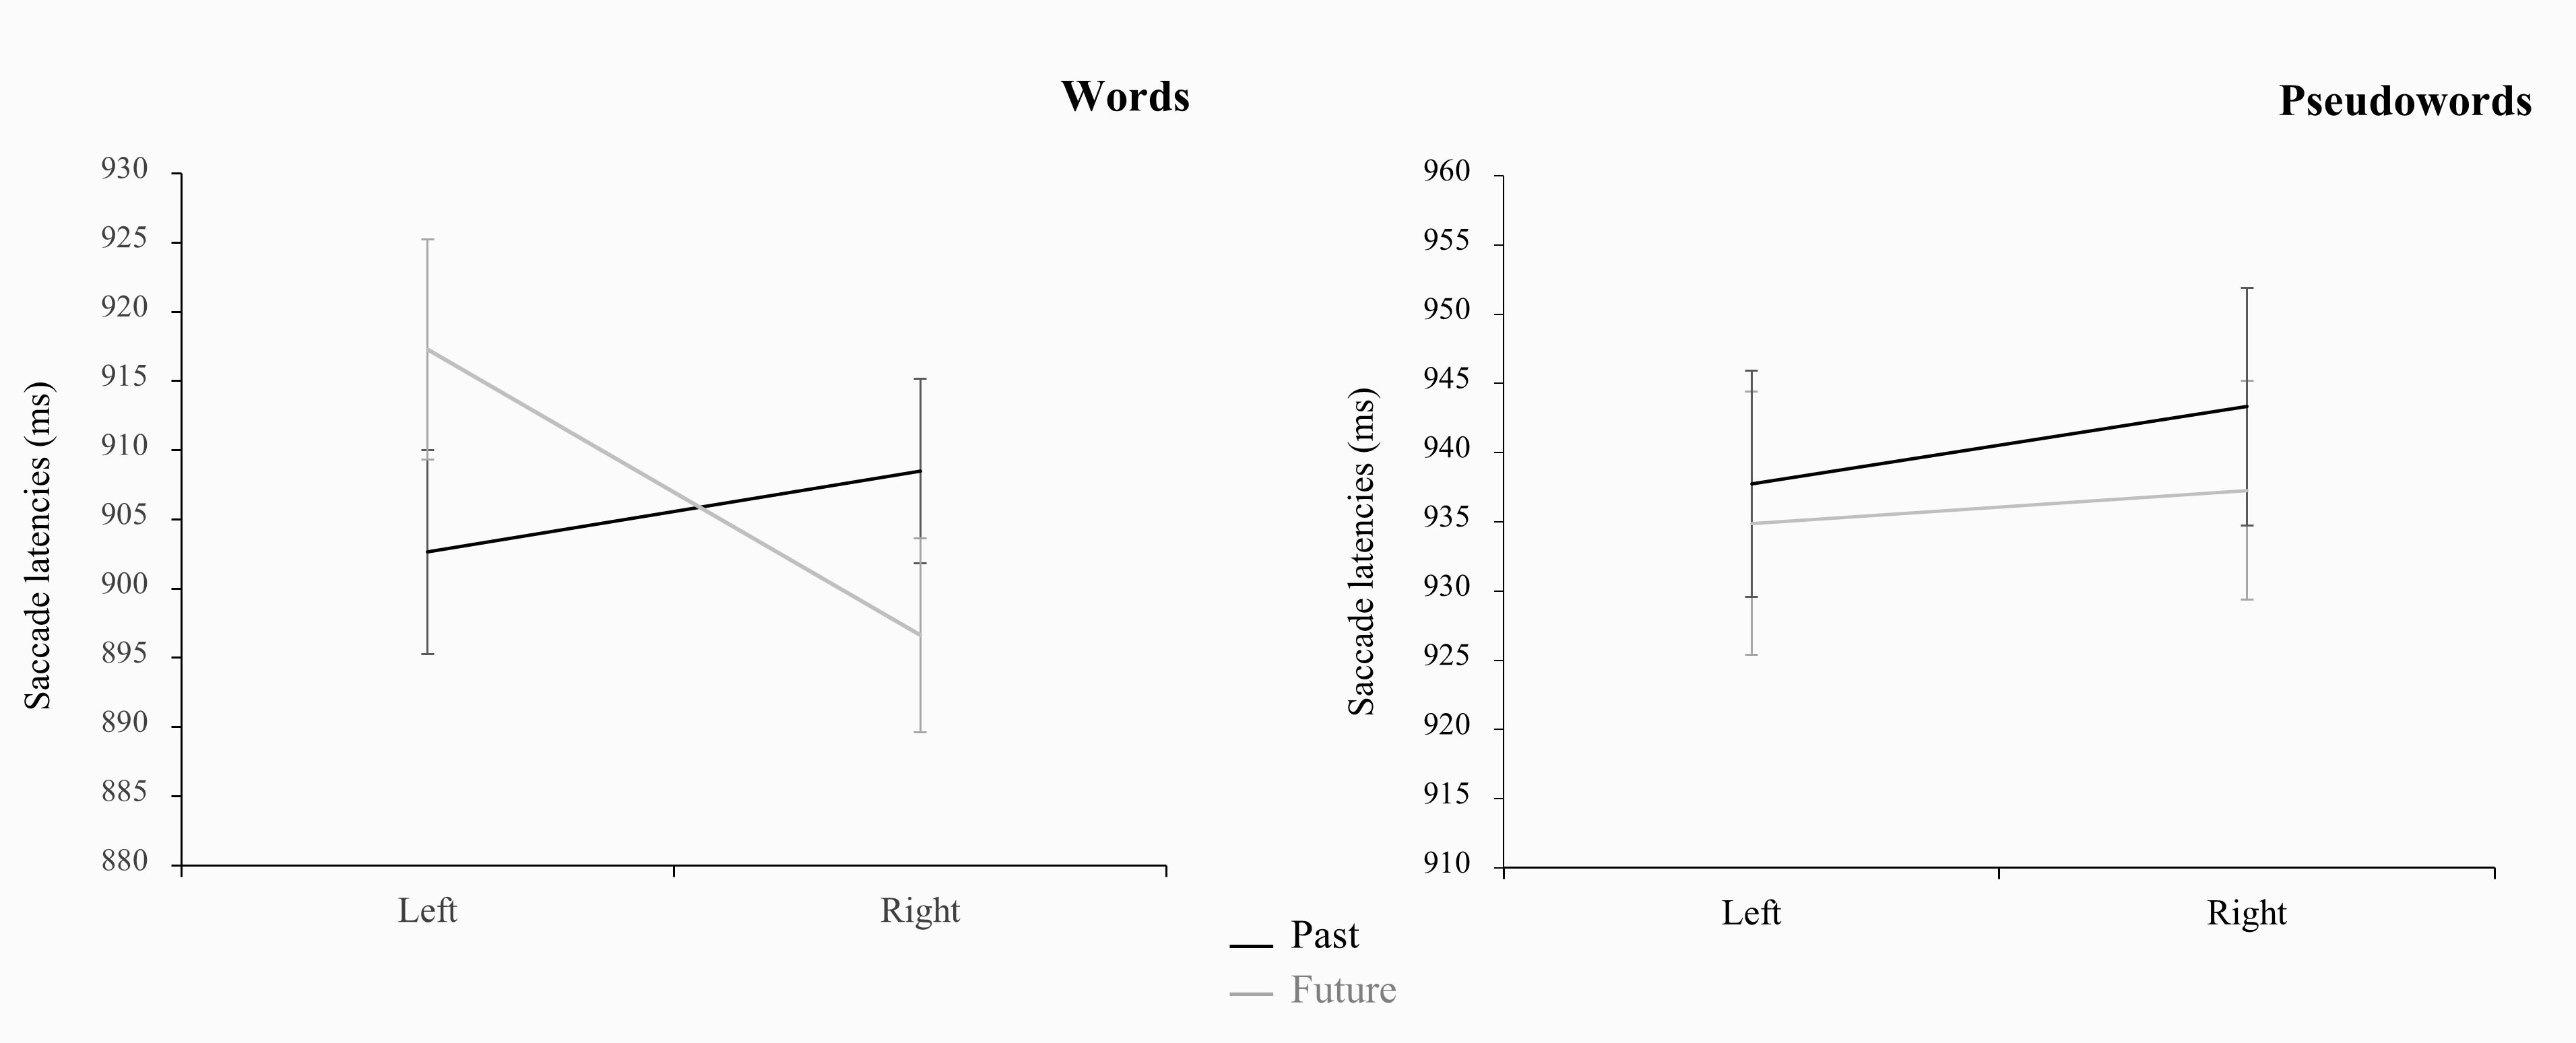
\includegraphics[width=1\linewidth]{figures/chap-4-fig2} 

}

\caption{Estimated marginal means from the mixed models (EMMs) for saccade latencies showing the interaction between Time (past vs future) and Side (left vs right) for words but not pseudowords. Error bars represent within subjects’ standard errors.}\label{fig:chap-4-fig2}
\end{figure}

\begin{figure}[htbp!]

{\centering 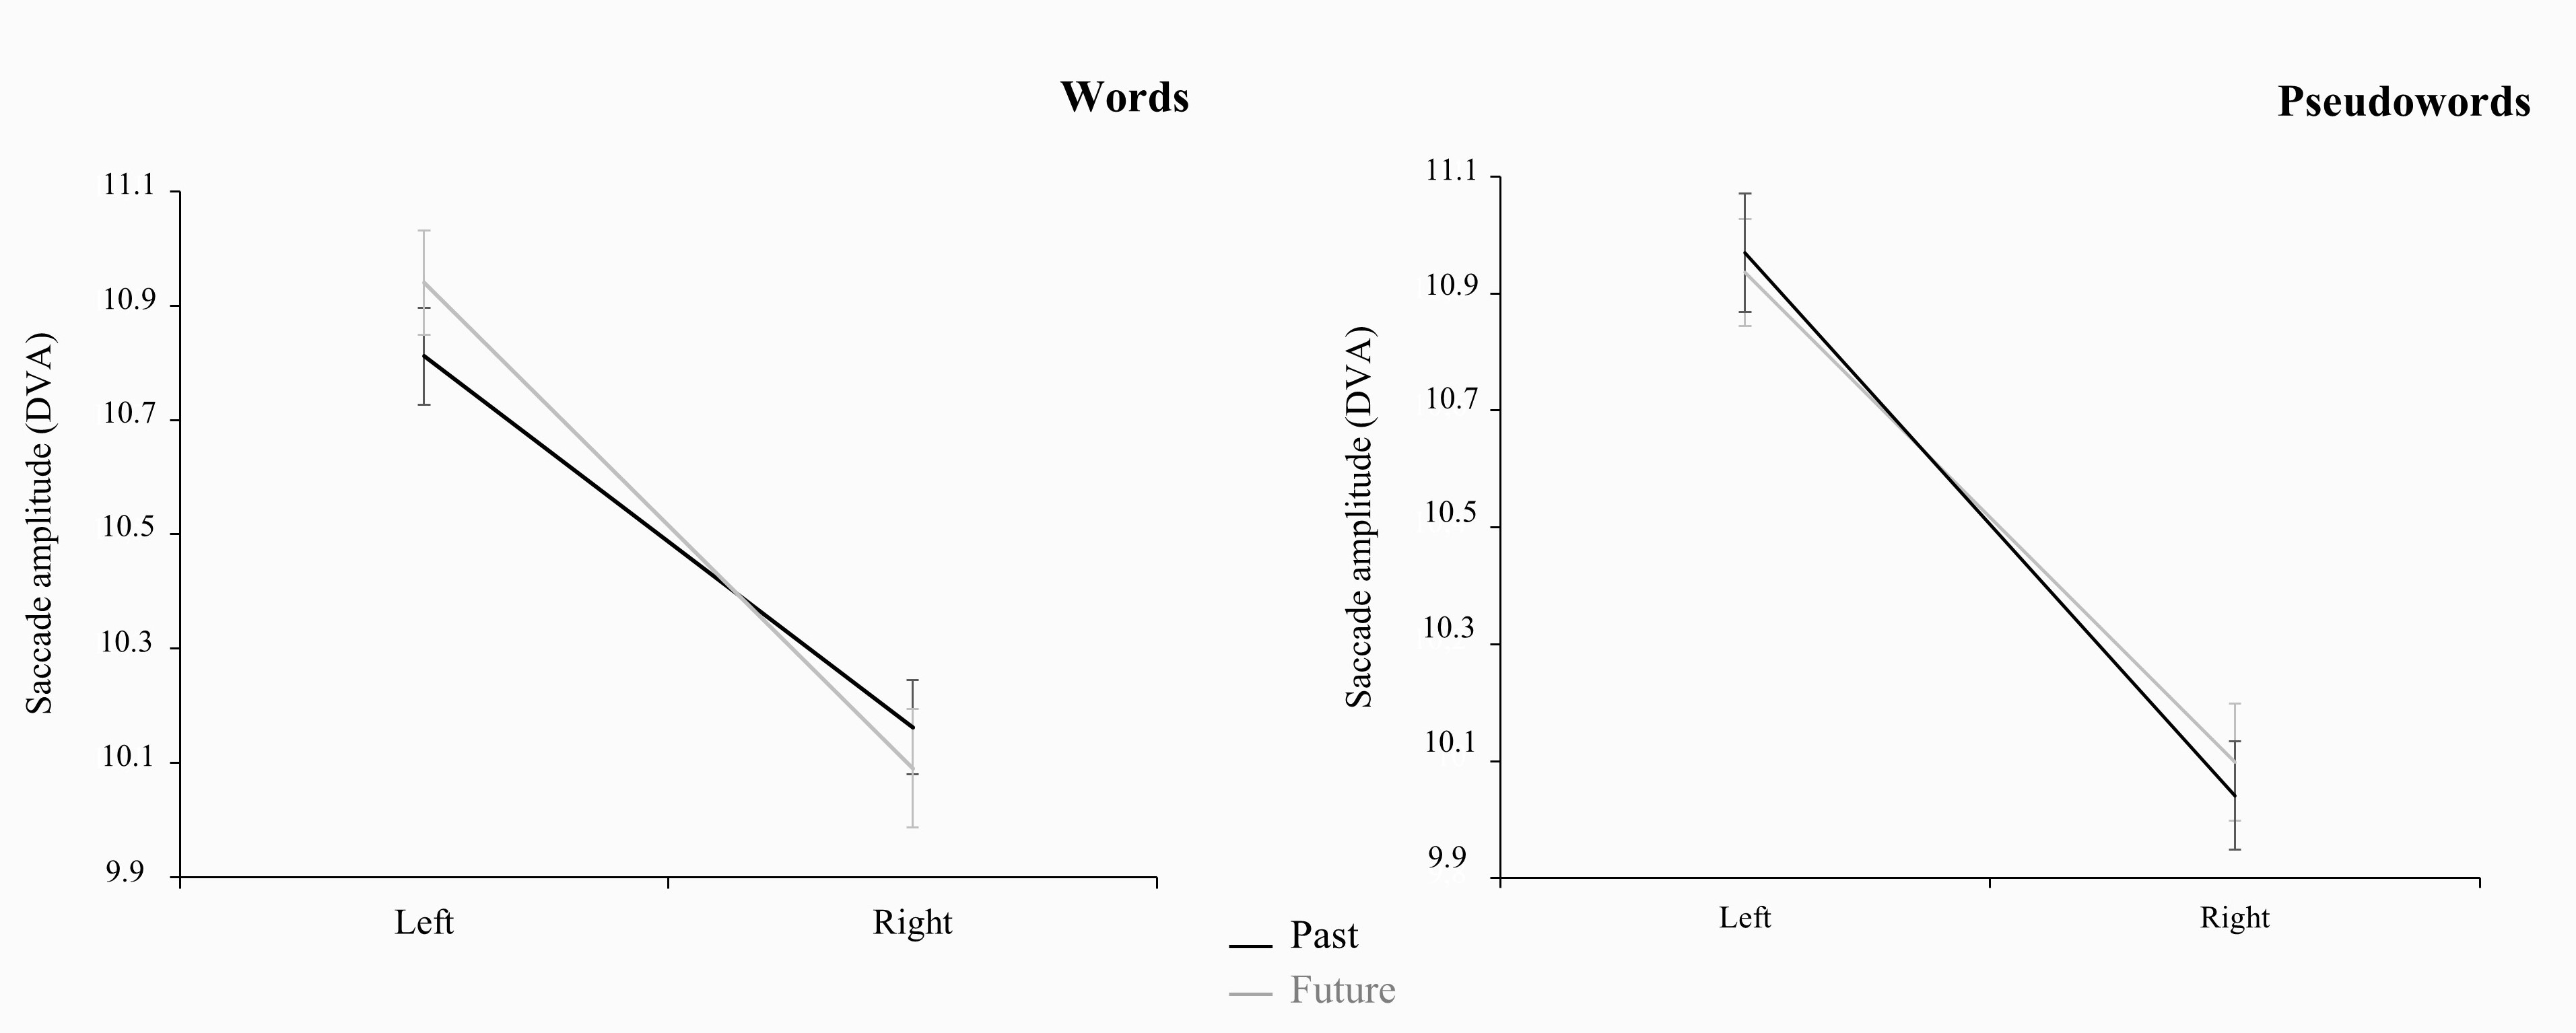
\includegraphics[width=1\linewidth]{figures/chap-4-fig3} 

}

\caption{Estimated marginal means from the mixed models (EMMs) for saccade amplitude showing the interaction between Time (past vs future) and Side (left vs right) for words but not pseudowords. Error bars represent within subjects’ standard errors. .}\label{fig:chap-4-fig3}
\end{figure}

\hypertarget{discussion-3}{%
\section{Discussion}\label{discussion-3}}

The primary purpose of the present study was to investigate whether the space-time congruency effect was effector-dependent (bound to the arm/hand) or would generalize to another effector. To this end, we used the same lexical decision task design as \protect\hyperlink{ref-grasso_as_2021}{Grasso, Ziegler, Mirault, et al.} (\protect\hyperlink{ref-grasso_as_2021}{2021}) but instead of using hand movements to register whether a stimulus was a real word or a pseudoword, participants made a saccade towards the left or right side of the screen. Congruent trials corresponded to leftwards eye-movements for past-tense words (or rightward for future-tense verbs) and incongruent trials to leftwards eye-movements for future-tense words (or rightward for past-tense verbs).

Our results replicate the space-time congruency effect for words in the lexical decision task when the eyes are used as response effectors. As in a previous study (\protect\hyperlink{ref-grasso_as_2021}{Grasso, Ziegler, Mirault, et al., 2021}), no such effect was found for pseudowords, which suggests that it taps into the nature of lexical word representations. The space-time congruency effect was observed for saccade latencies: leftward saccades were initiated more quickly for past-tense words, and the reverse pattern was found for future-tense words. In addition, a smaller but statistically significant space-time congruency effect was also found for saccade amplitude: participants made larger saccades on trials incongruent with the MTL. Saccade latency corresponds to the time needed to visually process the stimulus, to make the lexical decision, plus the time needed to program and launch the motor response (\protect\hyperlink{ref-gilchrist_saccades_2011}{Gilchrist, 2011}). Saccade amplitude is driven by the metrics and spatial parameters of the motor response. Therefore, the space-time congruency effect observed for saccade latencies can be considered an analog to the space-time congruency effect on lexical decision times previously obtained with hand responses. However, the space-time congruency effect for saccade amplitude is more likely driven by lexical interferences operating on the metrical adjustment and motor programming of the saccadic response. The parameters of the saccade cannot be modified once it is initiated (e.g., \protect\hyperlink{ref-edelman_influence_2007}{Edelman et al., 2007}; \protect\hyperlink{ref-gilchrist_saccades_2011}{Gilchrist, 2011}), which suggests that the calculation of the ballistic movement itself is affected by space-time incongruency. Note here that we did not make any prediction regarding the direction of the congruency effect on the amplitude of the saccade (i.e., shorter or longer saccade). The difference in amplitude between congruent and incongruent trials in itself shows that the processing of the temporal content of words interferes with saccade programming.

These results have three main theorical implications. First, they replicate our previous finding (\protect\hyperlink{ref-grasso_as_2021}{Grasso, Ziegler, Mirault, et al., 2021}) that a space-time congruency effect can be obtained when the processing of temporal information is not required to perform the task, which suggests that this effect taps into the lexical representations of words referring to time. As argued previously in the introduction, the key factor for obtaining this effect might be the involvement of spatially directed movement, and more precisely motor planning.

Second, whereas most studies observed space-time congruency effects when participants respond with their hands, here we obtain the same effect with the eyes, which strongly suggests that the spatial reference frame underlying the effect is centered on the body and refers to extra-personal space. Put another way, the generalization of the space-time congruency effect to eye movements suggests that the processing of words referring to time relies on extra-personal and egocentric spatial coordinates. This spatial reference frame, in which left-to-right movement through space is coded independently from the effector, might therefore be re-used for the purpose of representing words that convey temporal information. This spatial reference frame, probably underpinned by parietal cortex, is known as ``action-dependant'' and ``effector-independent'' (see for example, \protect\hyperlink{ref-heed_functional_2011}{Heed et al., 2011}).

Third and most important, the significant interaction between the temporal content of words and the direction of eye movements suggests that the very lexical representation of words that refer to time contains spatially oriented information (see also \protect\hyperlink{ref-hartmann_pupillometry_2014}{Hartmann \& Fischer, 2014}; \protect\hyperlink{ref-stocker_eye_2016}{Stocker et al., 2016}). Interference arises because, in the incongruent conditions, left or right response-movements activate spatially oriented motor networks that are incompatible with the oriented spatial-temporal information belonging to the lexical representation of the word. These results are congruent with the idea that the spatial representation of the temporal content of words derives from culture-dependent directional movements that are habitually produced during writing and reading (e.g., \protect\hyperlink{ref-bonato_when_2012}{Bonato et al., 2012}; \protect\hyperlink{ref-boroditsky_remembrances_2010}{Boroditsky \& Gaby, 2010}; \protect\hyperlink{ref-fuhrman_mental_2007}{Fuhrman \& Boroditsky, 2007}; \protect\hyperlink{ref-oliveri_representation_2009}{Oliveri et al., 2009}). More generally, our results suggest that words conveying temporal information are not abstract since they are grounded in spatially oriented movements of the motor effectors that are used to write or read. The spatial-temporal information that contributes to the representation of these words therefore appears to be action-driven, centered on the body (midline) and related to basic motor programs engaged during writing and reading.

\hypertarget{suppCh4}{%
\section{Supplementary materials}\label{suppCh4}}

Open data, supplementary materials, as well as reproducible code are available at \url{https://osf.io/5ehnc}.

Aside from previously cited packages, several other packages have been used for the writing of this paper, among which the \texttt{ggrepel} and \texttt{ggplot2} packages for plotting (\protect\hyperlink{ref-R-ggrepel}{Slowikowski, 2018}; \protect\hyperlink{ref-R-ggplot2}{Wickham et al., 2018}) as well as the \texttt{tidyverse}, \texttt{sjstats}, \texttt{here}, \texttt{skimr}, and \texttt{glue} packages for code writing and formatting (\protect\hyperlink{ref-R-glue}{Hester, 2017}; \protect\hyperlink{ref-R-sjstats}{Lüdecke, 2018}; \protect\hyperlink{ref-R-skimr}{McNamara et al., 2018}; \protect\hyperlink{ref-R-here}{K. Müller, 2017}; \protect\hyperlink{ref-R-tidyverse}{Wickham, 2017}).

\hypertarget{acknowledgements-1}{%
\section{Acknowledgements}\label{acknowledgements-1}}

We would like to thank Jonathan Mirault, Françoise Vitu and Boris Quetard for tremendously helpful comments and suggestions.

Camille Grasso was supported by a doctoral fellowship of the French Ministry of Higher Education, Research, and Innovation. This study benefited from support of the Institute of Convergence ILCB (ANR-16-CONV-0002) and the Excellence Initiative of Aix-Marseille University A*MIDEX (ANR-11-IDEX-0001-02).

\newpage

\begin{vplace}[1]

\begin{summary}{Résumé du Chapitre\getcurrentref{chapter}}{\chaptercolor}

Lorsque les individus prennent des décisions lexicales concernant des mots se référant au passé ou au futur, ils sont plus rapides lorsque leurs réponses manuelles sont compatibles avec la ligne mentale temporelle (effets de congruence spatio-temporelle). Les multiples observations de ces effets de congruence spatio-temporelle se sont traduites dans l’hypothèse selon laquelle les concepts abstraits temporels seraient conceptualisés spatialement le long d’un continuum allant de la gauche vers la droite (du passé vers le futur), du moins dans les cultures occidentales qui utilisent des systèmes de lecture-écriture organisés de gauche à droite. Les expériences précédentes utilisaient des réponses manuelles pour enregistrer les réponses, ce qui évoquait l’orientation spatiale de l'écriture. Pour évoquer celle de la lecture, nous avons étudié si l'effet de congruence spatio-temporelle serait reproduit dans une tâche de décision lexicale lorsque les réponses étaient données avec des mouvements oculaires dirigés vers la gauche ou vers la droite, plutôt qu’avec la main. Nous avons donc adapté les tâches de décision lexicales présentées dans le chapitre 3 à une tâche d’analyse de mouvements oculaires. Ces analyses ont montré une perturbation du temps d’initiation de la saccade et de son amplitude dans les conditions d’incongruence spatio-temporelle (e.g., mouvement gauche pour mot au futur). Nous avons interprété ces résultats en faveur de processus incarnés pour la représentation des concepts abstraits temporels. Précisément, nos résultats suggèrent que les mots désignant des concepts abstraits temporels pourraient prendre racine lors de mouvements spatialement dirigés d’une part, et que le cadre de référence spatial utilisé pour représenter ces derniers serait relatif au corps entier, plutôt que centré sur les effecteurs de la main. Enfin, ces résultats sont cohérents avec l'hypothèse d'un rôle du mouvement dynamique pour l'émergence d'effets de congruence spatio-temporelle lors d'une tâche temporelle implicite, ainsi qu'avec la proposition d’un rôle déterminant des expériences d’écriture et de lecture qui lieraient ensemble coordonnées spatiales et temporelles. La prochaine étude examinera deux questions. La première interroge le rôle des processus moteurs lors de tâches temporelles explicites (où les effets de congruence spatio-temporelle émergent même dans des conditions de réponses statiques). En effet, si le mouvement dynamique (i.e., spatialement dirigé) est déterminant pour émergence d’effets de congruence spatio-temporelle mesurables, pourquoi des conditions avec réponses statiques (i.e., pression de touches au clavier) lors de tâches temporelles explicites semblent suffisantes pour l’émergence d’effets mesurables ? La seconde interroge plus directement la relation entre organisation spatiale du temps - la ligne mentale temporelle - et expérience de lecture.  

\end{summary}

\end{vplace}

\changechaptercolor{hokusai5}

\hypertarget{chap5}{%
\chapter{Embodied time: Effect of reading expertise on the spatial representation of past and future}\label{chap5}}

\initial{H}ow do people grasp the abstract concept of time? It has been argued that abstract concepts, such as future and past, are grounded in sensory-motor experience. When responses to words that refer to the past or the future are either spatially compatible or incompatible with a left-to-right timeline, a space-time congruency effect is observed. In the present study, we investigated whether reading expertise would determine the strength of the space-time congruency effect, which would suggest that learning to read and write drives the effect. We compared two types of space-time congruency effects, one where spatial incongruency was generated by the location of the stimuli on the screen and one where it was generated by the location of the responses on the keyboard. While the first type of incongruency was visuo-spatial only, the second involved the motor system. Results showed stronger space-time congruency effects for the second type of incongruency (i.e., when the motor system was involved) than for the first type (visuo-spatial). Crucially, reading expertise, as measured by a standardized reading test, predicted the size of the space-time congruency effects. Altogether, these results reinforce the claim that the spatial representation of time is grounded in spatially-directed movement, such as reading or writing.\footnote{Ce chapitre expérimental est une version adaptée du manuscrit au format de la thèse. Pour trouver le préprint de la version soumise au journal Acta Psychologica: Les stimuli, les scripts, les données et les figures sont disponibles en ligne: \url{https://osf.io/g2k6z/}.}

\hypertarget{introduction-2}{%
\section{Introduction}\label{introduction-2}}

If abstract concepts are intangible, how could they be embodied through body-environment interactions? Embodied theories of language claim that concepts are represented through sensorimotor, interoceptive, and emotional networks that are activated when learning these concepts (e.g., \protect\hyperlink{ref-connell_interoception_2018}{Connell et al., 2018}; \protect\hyperlink{ref-vigliocco_neural_2014}{Vigliocco et al., 2014}; \protect\hyperlink{ref-villani_sensorimotor_2021}{Villani et al., 2021}). From this theoretical point of view, it is rather easy to conceive how the meaning of concrete words, such as \emph{book}, could be embodied through sensorimotor experience (e.g., since books are usually handled manually, hearing or reading this word supposedly activates hand-related motor networks; for some empirical evidence see for example \protect\hyperlink{ref-hauk_somatotopic_2004}{Hauk et al., 2004}; \protect\hyperlink{ref-pulvermuller_functional_2005}{Pulvermüller, Hauk, et al., 2005}). However, this is more complex for abstract concepts because we cannot physically ''grasp'' them through our senses, nor easily identify the cognitive experience during development that led to the representation of abstract words.

Consider for instance the abstract concept of time. Although we can feel and conceptualize it, time is an elusive construct devoid of any concrete phenomenology (e.g., \protect\hyperlink{ref-evans_structure_2003}{Evans, 2003}; \protect\hyperlink{ref-lakoff_philosophy_1999}{Lakoff \& Johnson, 1999}). There is no physical stimulus and no perceptual organ dedicated to time. In the absence of direct sensory experience of past and future, how could the brain construct a mental representation of time? One solution that has been proposed in the literature (e.g., \protect\hyperlink{ref-bergen_writing_2012}{Bergen \& Chan Lau, 2012}; \protect\hyperlink{ref-eikmeier_dimensional_2013}{Eikmeier et al., 2013}; \protect\hyperlink{ref-santiago_time_2007}{Santiago et al., 2007}) is that time is represented spatially, flowing linearly from one position in space to another. Thus, temporal cognition is thought to reuse neural structures devoted to spatial cognition.

This close link between space and time was theorized under the name of the mental timeline (for reviews see \protect\hyperlink{ref-bender_mapping_2014}{Bender \& Beller, 2014}; \protect\hyperlink{ref-bonato_when_2012}{Bonato et al., 2012}; \protect\hyperlink{ref-nunez_tangle_2013}{Núñez \& Cooperrider, 2013}). The mental timeline (MTL) refers to the phenomenon whereby individuals represent the temporal content of verbal stimuli (e.g., past and future) in two spatial axes that are centered on the body: for example, back-to-front (i.e., past in the back and future in the front; (e.g., \protect\hyperlink{ref-miles_mapping_2010}{Miles et al., 2010}; \protect\hyperlink{ref-sell_processing_2011}{Sell \& Kaschak, 2011}; \protect\hyperlink{ref-torralbo_flexible_2006}{Torralbo et al., 2006}; \protect\hyperlink{ref-ulrich_past_2012}{Ulrich et al., 2012}) and left-to-right (i.e., past on the left and future on the right (e.g., \protect\hyperlink{ref-bergen_writing_2012}{Bergen \& Chan Lau, 2012}; \protect\hyperlink{ref-grasso_as_2021}{Grasso, Ziegler, Mirault, et al., 2021}; \protect\hyperlink{ref-santiago_time_2007}{Santiago et al., 2007}; \protect\hyperlink{ref-weger_time_2008}{Weger \& Pratt, 2008}). Empirical evidence for the MTL comes from experiments that manipulated congruency between the temporal content of verbal stimuli and the spatial position of the required response, resulting in a space-time congruency effect (e.g., \protect\hyperlink{ref-bender_mapping_2014}{Bender \& Beller, 2014}; \protect\hyperlink{ref-bonato_when_2012}{Bonato et al., 2012}; \protect\hyperlink{ref-lewandowska-tomaszczyk_mental_2016}{Eikmeier et al., 2016}; \protect\hyperlink{ref-li_back_2019}{Li et al., 2019}). In various word or sentence processing tasks investigating the left-to-right MTL, left-hand responses are typically faster than right-hand ones for past-tense stimuli and right-hand responses are faster than left-hand ones for future-tense stimuli (e.g., \protect\hyperlink{ref-eikmeier_response_2015}{Eikmeier, Hoppe, et al., 2015}; \protect\hyperlink{ref-kong_space-time_2012}{Kong \& You, 2012}; \protect\hyperlink{ref-santiago_time_2007}{Santiago et al., 2007}; \protect\hyperlink{ref-torralbo_flexible_2006}{Torralbo et al., 2006}; for word stimuli, \protect\hyperlink{ref-maienborn_we_2015}{Maienborn et al., 2015}; \protect\hyperlink{ref-walker_disentangling_2014}{Walker et al., 2014}, for sentence stimuli).Interestingly, Li et al.~(2018), showed that when people operate in their second language, bilinguals unconsciously retrieve irrelevant native language spatial representations that shape time conceptualization in real time. Further evidence for the implication of spatial neural networks in the representation of time comes from neuropsychological data in which hemispatial neglect patients who ignore the left side of space, also have difficulties representing past events (e.g., \protect\hyperlink{ref-anelli_effects_2018}{Anelli et al., 2018}; \protect\hyperlink{ref-saj_patients_2014}{Saj et al., 2014}).

More recently, the hypothesis according to which words referring to time automatically activate neural motor circuits involved in spatial processing has been questioned (see \protect\hyperlink{ref-von_sobbe_space-time_2019}{von Sobbe et al., 2019}, for a meta-analysis). The argument was based on the finding that a strong and robust space-time congruency effect was found only when participants were asked to make an explicit judgment about the temporal content of verbal stimuli (e.g., \protect\hyperlink{ref-maienborn_we_2015}{Maienborn et al., 2015}; \protect\hyperlink{ref-ouellet_is_2010}{Ouellet, Santiago, Israeli, et al., 2010}; \protect\hyperlink{ref-santiago_time_2007}{Santiago et al., 2007}; \protect\hyperlink{ref-weger_time_2008}{Weger \& Pratt, 2008}). However, \protect\hyperlink{ref-grasso_as_2021}{Grasso, Ziegler, Mirault, et al.} (\protect\hyperlink{ref-grasso_as_2021}{2021}) have recently shown that robust space-time congruency effects can be observed even in an implicit temporal task (i.e., lexical decision about whether a word is real or not) as long as participants answer with a lateral movement of the hand. In four experiments, participants made lexical decisions to conjugated verbs or pseudoverbs and responded by either making spatially directed movements to the left or the right or by pressing a right or left response key. Space-time congruency effects occurred only for spatially directed movements, but not for button presses, regardless of whether the movement was performed with the hand (\protect\hyperlink{ref-grasso_as_2021}{Grasso, Ziegler, Mirault, et al., 2021}) or with the eyes (\protect\hyperlink{ref-grasso_eye_2021}{Grasso, Ziegler, Coull, et al., 2021}). These results suggested that left- or rightward movements through space are critical for observing the space-time congruency effect in implicit temporal tasks and therefore provide strong empirical support for automatic activation of motor planning networks in the (spatial) representation of time-related words.

The present study was designed to investigate two unresolved issues. First, if the activation of motor networks is critical for the occurrence of a space-time congruency effect during visual word processing, we hypothesized that the effect should be amplified when the space-time incongruency relies on the motor system (the left/right localisation of response keys) as opposed to when it relies only on the visual system (the left/right localisation of word stimuli on the screen). To test this hypothesis, we created incongruent associations (future to the left and past to the right) either on the screen (visual), or on the keyboard (motor) or both on the screen and the keyboard. Second, if the directionality of the MTL (future to the right and past to the left) is related to the directionality of reading and writing, we hypothesized that reading expertise should correlate positively with the size of the space-time congruency effect.

As concerns the second hypothesis, it has been suggested that the left-to-right MTL in western languages results from motor experience related to reading and writing. During writing, our hands, eyes, and attention move spatially from left to right, gradually shifting from what has been read/written - the past - to what will be read/written -the future- (e.g., \protect\hyperlink{ref-hutchison_can_2010}{Casasanto \& Bottini, 2010}; \protect\hyperlink{ref-fuhrman_mental_2007}{Fuhrman \& Boroditsky, 2007}; \protect\hyperlink{ref-pitt_reading_2016}{Pitt \& Casasanto, 2016}). Empirically, this hypothesis is based on a large amount of cross-cultural data showing that the direction of the space-time congruency effect follows the direction of the participants' writing system (e.g., \protect\hyperlink{ref-fuhrman_mental_2007}{Fuhrman \& Boroditsky, 2007}; \protect\hyperlink{ref-ouellet_is_2010}{Ouellet, Santiago, Israeli, et al., 2010}). Whereas in cultures that read and write from left to right, participants are faster to respond to past tense items with their left hand and future tense items with their right hand (e.g., \protect\hyperlink{ref-kong_space-time_2012}{Kong \& You, 2012}; \protect\hyperlink{ref-santiago_time_2007}{Santiago et al., 2007}; \protect\hyperlink{ref-torralbo_flexible_2006}{Torralbo et al., 2006}; \protect\hyperlink{ref-ulrich_leftright_2010}{Ulrich \& Maienborn, 2010}; \protect\hyperlink{ref-walker_spatial_2017}{Walker et al., 2017}; \protect\hyperlink{ref-weger_time_2008}{Weger \& Pratt, 2008}), the reverse pattern is found for participants whose writing system operates from right-to-left (e.g., Hebrew scripts, \protect\hyperlink{ref-fuhrman_mental_2007}{Fuhrman \& Boroditsky, 2007}). \protect\hyperlink{ref-casasanto_spatial_2014}{Casasanto \& Bottini} (\protect\hyperlink{ref-casasanto_spatial_2014}{2014}) were the first to directly assess the causal influence of reading expertise on the space-time congruency effect. In their study, Dutch participants had to judge the temporal content of sentences written either in a standard direction or in a mirror-reversed direction. Results revealed that the direction of space-time associations followed the direction of eye and hand movements: that is, left-past and right-future associations when participants had to read sentences in the standard left-to-right direction, and right-past and left-future associations when participants had to read sentences in the right-to-left direction (for another exemple, see \protect\hyperlink{ref-pitt_reading_2016}{Pitt \& Casasanto, 2016}). These space-time congruency effects suggest that reading experience plays a role in the direction in which time is spatially represented.

If the abstract concept of time is grounded in the directional movements performed during reading and writing, then the space-time congruency effect should correlate positively with the degree of reading and writing expertise of the participants: more experienced readers should be more sensitive to space-time incongruities. Recently, the link between reading expertise and the processing of temporal order (i.e., before vs.~after) was investigated in a developmental study using non-verbal stimuli (\protect\hyperlink{ref-autry_development_2020}{Autry et al., 2020}). Participants, ranging from preschoolers to adults, had to represent the temporal order of coloured circles presented sequentially on a computer by placing coloured cards in front of them (\protect\hyperlink{ref-autry_development_2020}{Autry et al., 2020}). Results revealed a left-to-right bias in organizing the order of events, even in preschoolers. Crucially, results showed that the more children were familiar with reading, the more they organized the temporal order of events from left-to-right. Nevertheless, the claim that the depth of reading and writing experience correlates with the strength of the spatial representation of past and future words still lacks direct empirical evidence.

Based on these theoretical and empirical considerations, the present study was designed to investigate the role of motor function and reading expertise in the space-time congruency effect that is observed during lexical processing of the abstract concept of time (i.e., past and future related words). One way to investigate the role of motor function in the space-time congruency effect is to manipulate whether congruency occurs at the perceptual (visual) or motor level. For instance, in \protect\hyperlink{ref-santiago_time_2007}{Santiago et al.} (\protect\hyperlink{ref-santiago_time_2007}{2007}) participants had to categorize past and future words presented either on the left or right side of the screen, and to make lateralized static keyboard responses using their left or right hand. Two types of space-time congruency were manipulated. First, the congruency between the temporal content of the stimuli (past/future) and the left/right spatial location of the stimuli on the screen (i.e., perceptual congruency on screen), which is independent of motor execution. Second, the congruency between the temporal content of the stimuli and the left/right spatial location of responses on the keyboard, which depends on motor execution (i.e., motor congruency on the keyboard). Participants performed the same temporal categorisation twice: once with congruent key responses, and once with incongruent key responses in a counterbalanced order. Space-time congruency effects occurred in both the perceptual and motor conditions, suggesting that incongruency on either the screen or the keyboard can interfere with performance. However, in Santiago's et al.~study, no comparative analysis between these two space-time congruency conditions was conducted. In the present study, we will directly compare the effect size of the two conditions.

To investigate the role of reading expertise in the space-time congruency effect - and thus the spatial representation of time -, we included two reading proficiency measures. First, we used a French version of a computerized reading test which measures both reading comprehension and reading speed of sentences (i.e., SLS-Berlin, \protect\hyperlink{ref-ludtke_sls-berlin_2019}{Lüdtke et al., 2019}). It has been shown that the SLS-Berlin is an excellent tool for screening interindividual variability in reading expertise (\protect\hyperlink{ref-ludtke_sls-berlin_2019}{Lüdtke et al., 2019}). Second, to assess language proficiency, we used the Lextale\_FR (\protect\hyperlink{ref-brysbaert_lextale_fr_2013}{Brysbaert, 2013}) commonly used in the literature to screen participants' vocabulary size.

In sum, the present study was designed to investigate in a single explicit temporal task the role of motor function and reading expertise in the space-time congruency effect. Since we replicate the experiment by \protect\hyperlink{ref-santiago_time_2007}{Santiago et al.} (\protect\hyperlink{ref-santiago_time_2007}{2007}), we should observe the same pattern of results; that is, space-time congruency effects in both the screen and the keyboard conditions. Furthermore, since recent work suggests that motor planning plays a crucial role in lexical processing of the temporal content of words (e.g., \protect\hyperlink{ref-grasso_as_2021}{Grasso, Ziegler, Mirault, et al., 2021}; \protect\hyperlink{ref-grasso_eye_2021}{Grasso, Ziegler, Coull, et al., 2021}), we predicted a stronger space-time congruency effect size in the keyboard-congruent condition as compared to the screen-congruent condition. Finally, we predicted a positive correlation between the size of the space-time congruency effect and reading expertise.

\hypertarget{materials-and-methods-1}{%
\section{Materials and Methods}\label{materials-and-methods-1}}

\hypertarget{participants-4}{%
\subsection{Participants}\label{participants-4}}

Since one of the main objectives of the present study was to assess the link between reading expertise and the space-time congruency effect, we conducted the study in a wide range of ages in the general population rather than in undergraduate psychology students. This was done to increase inter-individual differences in reading expertise. Thus, ninety adults ranging in age from 18 to 72 years old participated in the experiment. Four adults were not included in the final analyses due to high error rate (i.e., \textgreater15\%). Three others participants had abnormal or aberrant RT distributions (many very fast or slow responses, or huge variability) and the data from these participants were excluded from the final analysis. The remaining 83 participants (36 women, 70 right-handed) were all French native speakers, reported normal or corrected-to-normal vision and ranged in age from 18 to 72 years old (\emph{M} = 30.69; \emph{SD} = 10.97). All participants were recruited online, through the Prolific.ac website and received 10€/hours for their participation. The study was conducted in accordance with the recommendations of the World Medical Association Declaration of Helsinki, and it approved by the Institutional Review Board of Aix-Marseille University.

\hypertarget{design-and-stimuli-2}{%
\subsection{Design and Stimuli}\label{design-and-stimuli-2}}

We selected 84 past tense conjugated verbs and 84 future tense conjugated verbs from the Lexique 3 database (\protect\hyperlink{ref-new_lexique_2004}{New et al., 2004}). Past and future words were matched with respect to length (7.92 versus 7.99 letters, \emph{p} = .65, for past versus future words, respectively) and frequency (19.27 versus 8.42 occurrences per million, \emph{p} = .11, for past versus future words, respectively). We used a Latin-Square design for creating 4 lists of 168 stimuli each (84 past words and 84 future words). Half of the past- or future- words could appear on the left of the screen and the other half on the right. For each session, participants saw one of the four lists, with each word presented once only and in random order.

\hypertarget{apparatus-2}{%
\subsection{Apparatus}\label{apparatus-2}}

The experiment was programmed in PHP, JAVASCRIPT, and HTML, and was made available online. All participants performed the online experiment on their own personal computer and were asked to respond with their keyboard by pressing the ``S'' key for left-responses with their left-hand or the ``L'' key for right-responses with their right hand (AZERTY keyboard). All words were presented in 30-point arial font in black on a white background. When opening the web link of the online experiment, each participant was assigned to one of the four lists. We collected latencies (i.e., time between the onset of the stimulus and participants' responses) measured with millisecond precision (see Figure \ref{fig:chap-5-fig1}).

\begin{figure}[htbp!]

{\centering 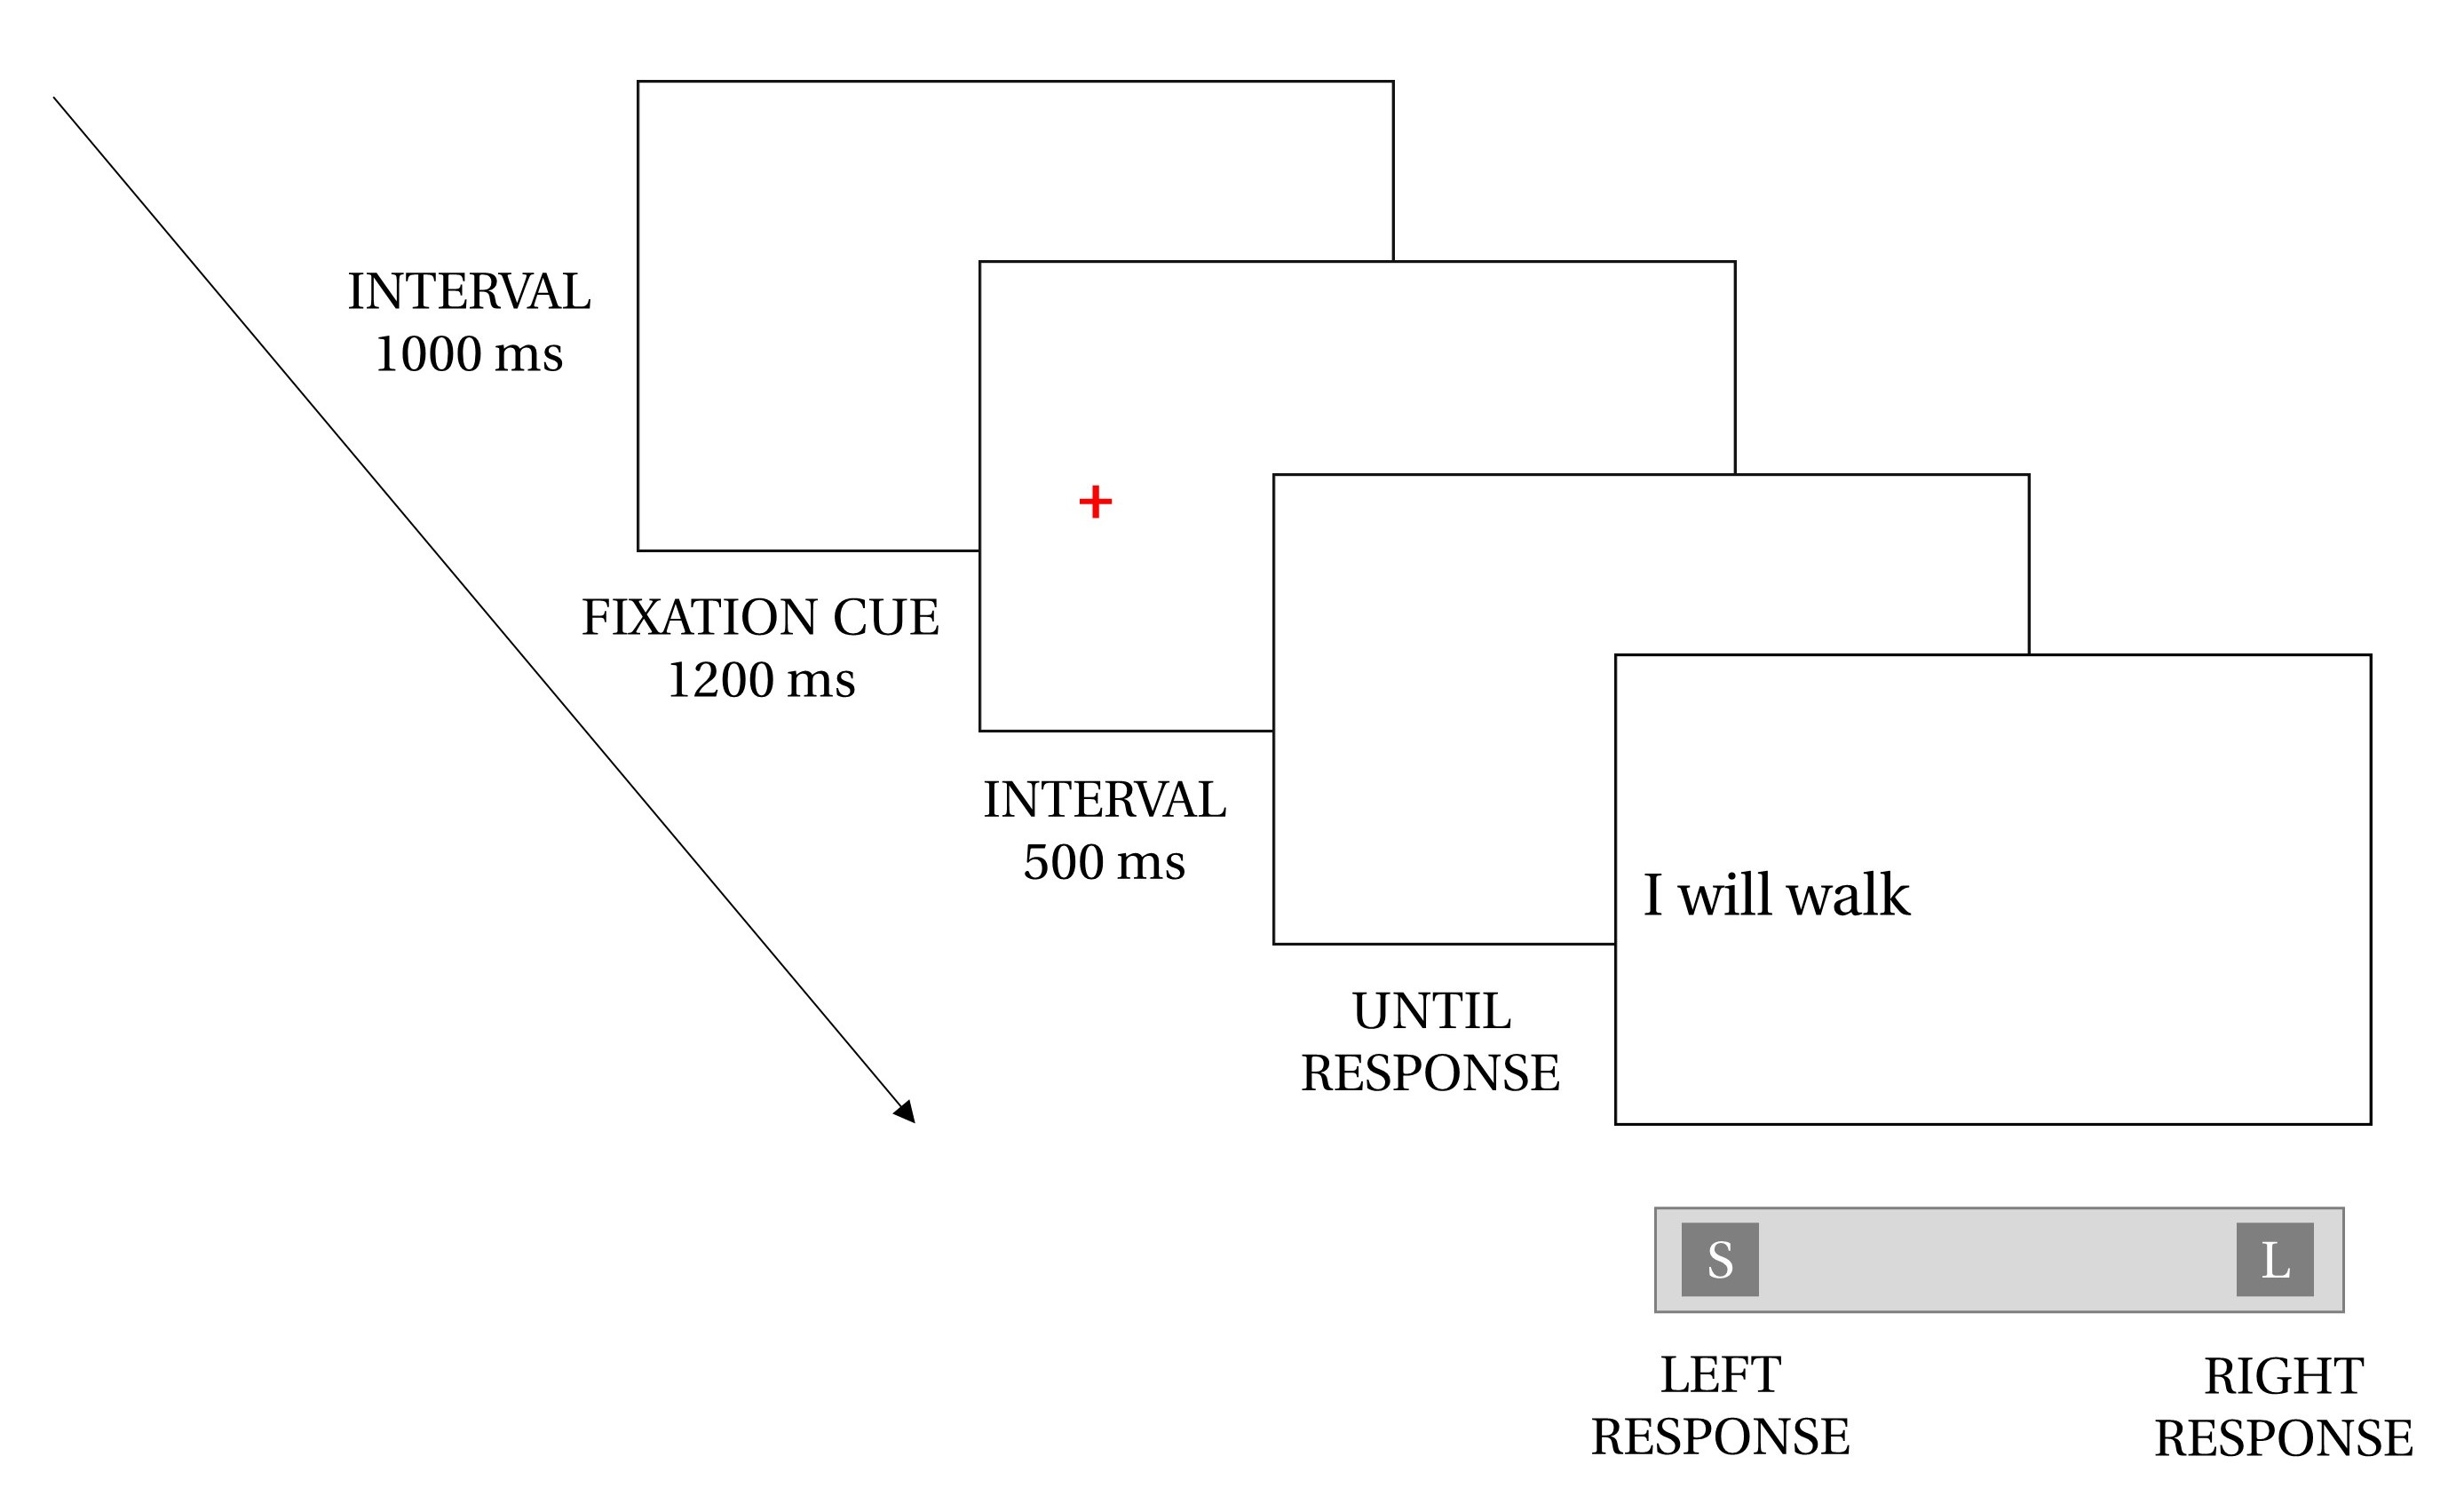
\includegraphics[width=1\linewidth]{figures/chap-5-fig1} 

}

\caption{Experimental design. Words were displayed after a spatial fixation cue. Participants made their temporal categorization by pressing the left or the right response key (i.e., “S” and “L” key) on an AZERTY keyboard.}\label{fig:chap-5-fig1}
\end{figure}

\hypertarget{procedure-2}{%
\subsection{Procedure}\label{procedure-2}}

The experiment consisted of a temporal categorization task (does the stimulus refer to the past or the future?). Detailed instructions were displayed when opening the web link of the experiment. Participants were asked to perform the experiment in a quiet environment with no acoustic or visual distractions, and to start the task after completing a demographic questionnaire (i.e., age, gender, education level and dominant hand for writing). The experiment consisted of two independent sessions of 168 trials each, separated by 5 days and lasted for approximately 15 minutes. A participation link for the second session was sent to the participants 5 days after the first session. The tasks (temporal categorization) in both sessions were strictly identical except for the key response mapping, that is, in one session, the left-past and right-future response represented a space-time congruent key mapping, whereas in the other session the left-future and right-past response represented a space-time incongruent key mapping. The order of presentation of key response mapping was counterbalanced across participants. Instructions explained that words would appear either on the left or right side of the screen, which would always be preceded by a red cross to indicate where the word would appear. All participants were instructed to decide as rapidly and as accurately as possible whether the stimulus was a past- or future-word by pressing the left- or right-key of an AZERTY keyboard with their left and right hands, respectively. For each session, participants saw a total of 84 past-tense words and 84 future-tense words, presented in random order with half of each on the left of the screen and half on the right. As can be seen in Figure \ref{fig:chap-5-fig1}, at the beginning of each trial, a red fixation cross was displayed for 1200ms on the side where the word would appear, followed by a blank display for 500ms and then the stimulus (e.g., I drew) remained on the screen until the participants' response. Participants were asked to stop answering when they felt the need to take a break, and to resume when ready.

Note that independently of the type of stimuli presented, the combination of left-right stimulus locations on the screen together with left-right key responses could trigger the well-known Simon compatibility effect (e.g., \protect\hyperlink{ref-simon_effect_1990}{Simon \& Berbaum, 1990}; \protect\hyperlink{ref-zorzi_computational_1995}{Zorzi \& Umiltà, 1995}). When asked to produce a response at a location that is congruent with the spatial location of the stimulus on the screen (e.g., left key response for a left-sided stimulus), participants give faster responses than in incongruent trials (e.g., right key response for a left-sided stimulus). Although \protect\hyperlink{ref-santiago_time_2007}{Santiago et al.} (\protect\hyperlink{ref-santiago_time_2007}{2007}) found no interaction between stimulus location on the screen and response location on the keyboard, which suggests the absence of a Simon effect, we added Simon congruency as a predictor in our statistical analyses to isolate space-time congruency from the (non-temporal) Simon effect. Altogether, the experiment therefore comprised four congruency conditions summarized as the A, B, C and D conditions, as depicted in Figure \ref{fig:chap-5-fig2}. All stimuli can be found in the Supplementary Materials.

\begin{figure}[htbp!]

{\centering 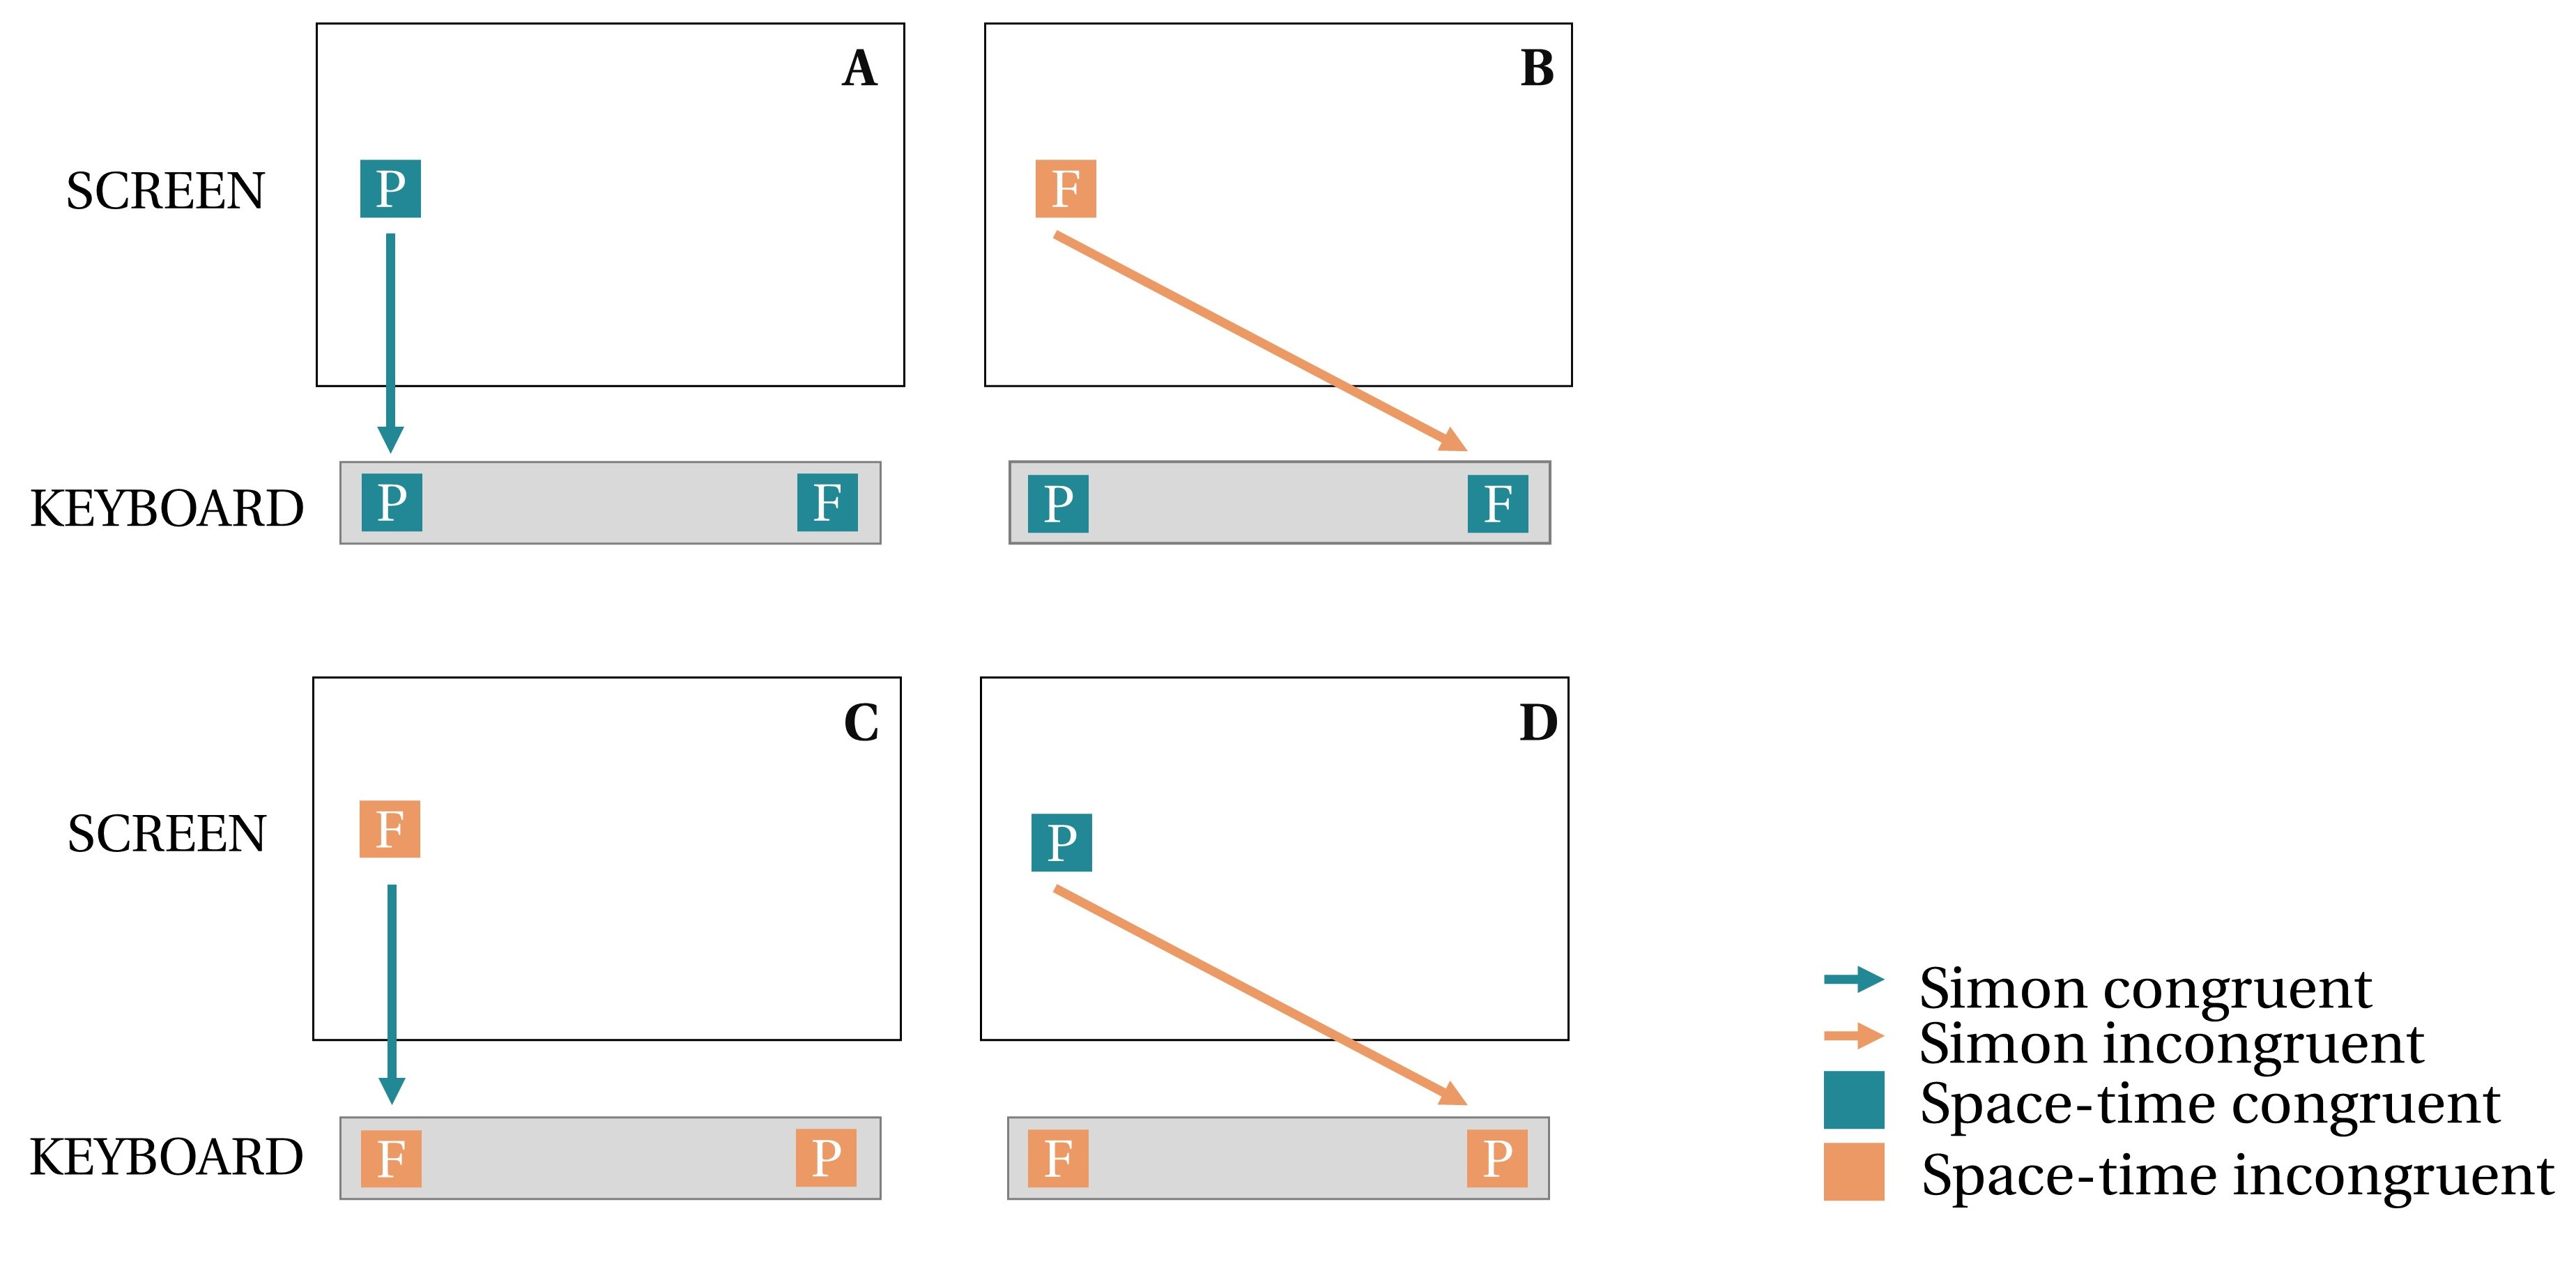
\includegraphics[width=1\linewidth]{figures/chap-5-fig2} 

}

\caption{Congruency conditions. A and B correspond to keyboard congruent conditions, C and D correspond to keyboard incongruent conditions.  In an orthogonal manner, A and D correspond to screen congruent conditions, B and C correspond to screen incongruent conditions. Finally, A and C correspond to Simon congruent conditions and B and D correspond to Simon incongruent conditions. Note. P: past-tense stimulus. F: future-tense stimulus.  The figure illustrates the four congruency conditions for left-sided stimuli.  Four equivalent conditions were also presented for right-sided stimuli.}\label{fig:chap-5-fig2}
\end{figure}

To assess language proficiency, participants completed the Lextale\_FR (\protect\hyperlink{ref-brysbaert_lextale_fr_2013}{Brysbaert, 2013}). After the categorisation task in the first session, a link automatically redirected participants to the Lextale\_FR (\protect\hyperlink{ref-brysbaert_lextale_fr_2013}{Brysbaert, 2013}). This task consists of fixed presentation of 120 words and pseudowords in the centre of the screen, separated by a 1200ms blank screen. Participants had to decide whether the words exist by pressing the left or right key on their personal keyboard. Reading proficiency was measured by the French version of the SLS-Berlin in the second session (\protect\hyperlink{ref-ludtke_sls-berlin_2019}{Lüdtke et al., 2019}). After the categorisation task in the second session, a link automatically redirected participants to the SLS-Berlin (\protect\hyperlink{ref-ludtke_sls-berlin_2019}{Lüdtke et al., 2019}). The French version of the SLS-Berlin consisted of the successive presentation of 77 correct or incorrect sentences (e.g., ``Drunk drivers have a slower reaction time.'' or ``A rhinoceros is a wind instrument.'' respectively) at the centre of the screen, separated by a 1200ms blank screen and in a fixed order. Participants were asked to judge the plausibility or implausibility of the sentences by pressing a left or right key on their keyboard. The task stopped automatically after 3 minutes of sentence presentation (this duration did not include inter-stimulus intervals).

\hypertarget{data-analysis}{%
\subsection{Data analysis}\label{data-analysis}}

We recorded and analyzed response accuracy (error rates, in percentage) and response latency (in milliseconds), that is the time interval between the onset of the stimulus and participants' keyboard response. Aberrant values corresponding to trials with latencies greater than 4000ms and less than 250ms (0.58\% of trials) were discarded from the analyses. Response latencies were all inverse transformed (-1000 / RT) and predictors of participants' reading expertise (measured by the Lextale\_FR and the SLS\_Berlin) were standardized prior to analyses.

Analyses of accuracy and latencies (for correct responses) were conducted with linear mixed-effects models (\protect\hyperlink{ref-baayen_mixed-effects_2008}{Baayen et al., 2008}) using the \texttt{lmer()} and \texttt{glmer()} functions from the \texttt{lme4} package (\protect\hyperlink{ref-bates_fitting_2015}{Bates et al., 2015}) in the \texttt{R} statistical computing environment (\protect\hyperlink{ref-r_core_team_r_2020}{R Core Team, 2020}). We report unstandardized regression coefficients (b), standard errors (SEs), \textbar t\textbar{} or \textbar F\textbar{} values (for lmer), \textbar z\textbar{} values (for glmer), standardized mean difference (SMD, effect size), and corresponding p-values. For multilevel predictors (e.g., condition), we report the F-values of the main effect, standard errors (SEs) and corresponding p-values computed with the anova() function from the lmerTest package (\protect\hyperlink{ref-kuznetsova_lmertest_2017}{Kuznetsova et al., 2017}). We also report unstandardized regression coefficients (b), \textbar Z\textbar{} values and corresponding p-values for contrasts analyses computed with the \texttt{pairwise()} function from the \texttt{emmeans} package (\protect\hyperlink{ref-lenth_emmeans_2021}{Lenth, 2021}). Regarding model building, we used the maximal random structure model that reached convergence (\protect\hyperlink{ref-barr_random_2013}{Barr, 2013}). The final model included by-participant and by-item random intercepts in all analyses that we report. In a forward stepwise model selection procedure, fixed and random effects of the models were selected according to the Akaike Information Criterion (AIC, \protect\hyperlink{ref-akaike_maximum_1973}{Akaike, 1973}), the Bayesian Information Criterion (BIC, \protect\hyperlink{ref-schwarz_estimating_1978}{Schwarz, 1978}), and the chi-squared log-likelihood ratio tests with regular maximum likelihood parameter estimation using the \texttt{anova()} function of the \texttt{lmerTest} package (\protect\hyperlink{ref-kuznetsova_lmertest_2017}{Kuznetsova et al., 2017}) for model comparison. Therefore, fixed effects, random effects, and random slopes were only included if they significantly improved the model's fit. Assumptions of the model were checked for each model: the normality of the residual distribution and dispersion were inspected using the \texttt{simulateresiduals()} function from the \texttt{DHARMa} (\protect\hyperlink{ref-hartig_dharma_2021}{Hartig, 2021}) package for \texttt{glmer} models, and residual distribution were checked visually by plotting the residuals' \texttt{Quantile-Quantile} (QQ) and the normality of the distribution of the random effects by plotting the QQ-plots with the \texttt{qqmath()} function (from \texttt{Lattice} package, \protect\hyperlink{ref-sarkar_lattice_2008}{Sarkar, 2008}) and the \texttt{ranef()} function for \texttt{lmer} models. Effect sizes for each predictor of the model were computed using the \texttt{eff\_size()} function of the \texttt{emmeans} package (\protect\hyperlink{ref-lenth_emmeans_2021}{Lenth, 2021}). The \texttt{eff\_size()} function computes a standardised mean difference, using pairwise differences of estimates divided by the (estimated) standard deviation of the population.To create figures, we used the \texttt{emmeans} package (\protect\hyperlink{ref-lenth_emmeans_2021}{Lenth, 2021}) that allowed us to compute the estimated marginals means (EMMs) for each model (see for instance Figure \ref{fig:chap-5-fig4}).

\hypertarget{results-4}{%
\section{Results}\label{results-4}}

\hypertarget{reaction-times}{%
\subsection{Reaction times}\label{reaction-times}}

The final model included Simon congruency (congruent vs.~incongruent), screen congruency (congruent vs.~incongruent), keyboard congruency (congruent vs.~incongruent), and participant age as fixed effects, as well as standardized reading expertise (expressed by the sum of correct responses in the SLS-Berlin) and its interaction with each type of congruency, and by-participant and by-time intercepts. Results revealed a marginal effect of age (\emph{b} = -0.01, \emph{SE} = 0.01, \emph{t} = 1.79, \emph{p} =.076), a significant effect of reading expertise (\emph{b} = -0.01, \emph{SE} = 0.01, \emph{t} = 3.79, \emph{p} \textless{} .001), a significant Simon congruency effect (\emph{b} = -0.01, \emph{SE} = 0.01, \emph{t} = 3.05, \emph{p} \textless{} .001, \emph{SMD} = 0.046), and a significant space-time congruency effect of key response mapping (\emph{b} = -0.01, \emph{SE} = 0.01, \emph{t} = 8.18, \emph{p} \textless{} .001, \emph{SMD} = 0.131) (Figure \ref{fig:chap-5-fig3}). However, there was no significant space-time congruency effect of screen location (\emph{b} = -0.01, \emph{SE} = 0.01, \emph{t} = 1.28, \emph{p} = .259, \emph{SMD} = 0.024). Interestingly, analyses revealed a significant interaction between reading expertise and space-time congruency of both key response mapping (\emph{b} = -0.01, \emph{SE} = 0.01, \emph{t} = 6.24, \emph{p} \textless{} .001) and screen location (\emph{b} = -0.00, \emph{SE} = 0.00, \emph{t} = 2.25, \emph{p} = .024), but no interaction with Simon congruency (\emph{b} = -0.01, \emph{SE} = 0.01, \emph{t} = 2.25, \emph{p} =.024). In other words, the better the reading expertise of the participants, the stronger the space-time congruency effect of the key response mapping and of the spatial location of the stimulus on screen (Figure \ref{fig:chap-5-fig3}).

\begin{figure}[htbp!]

{\centering 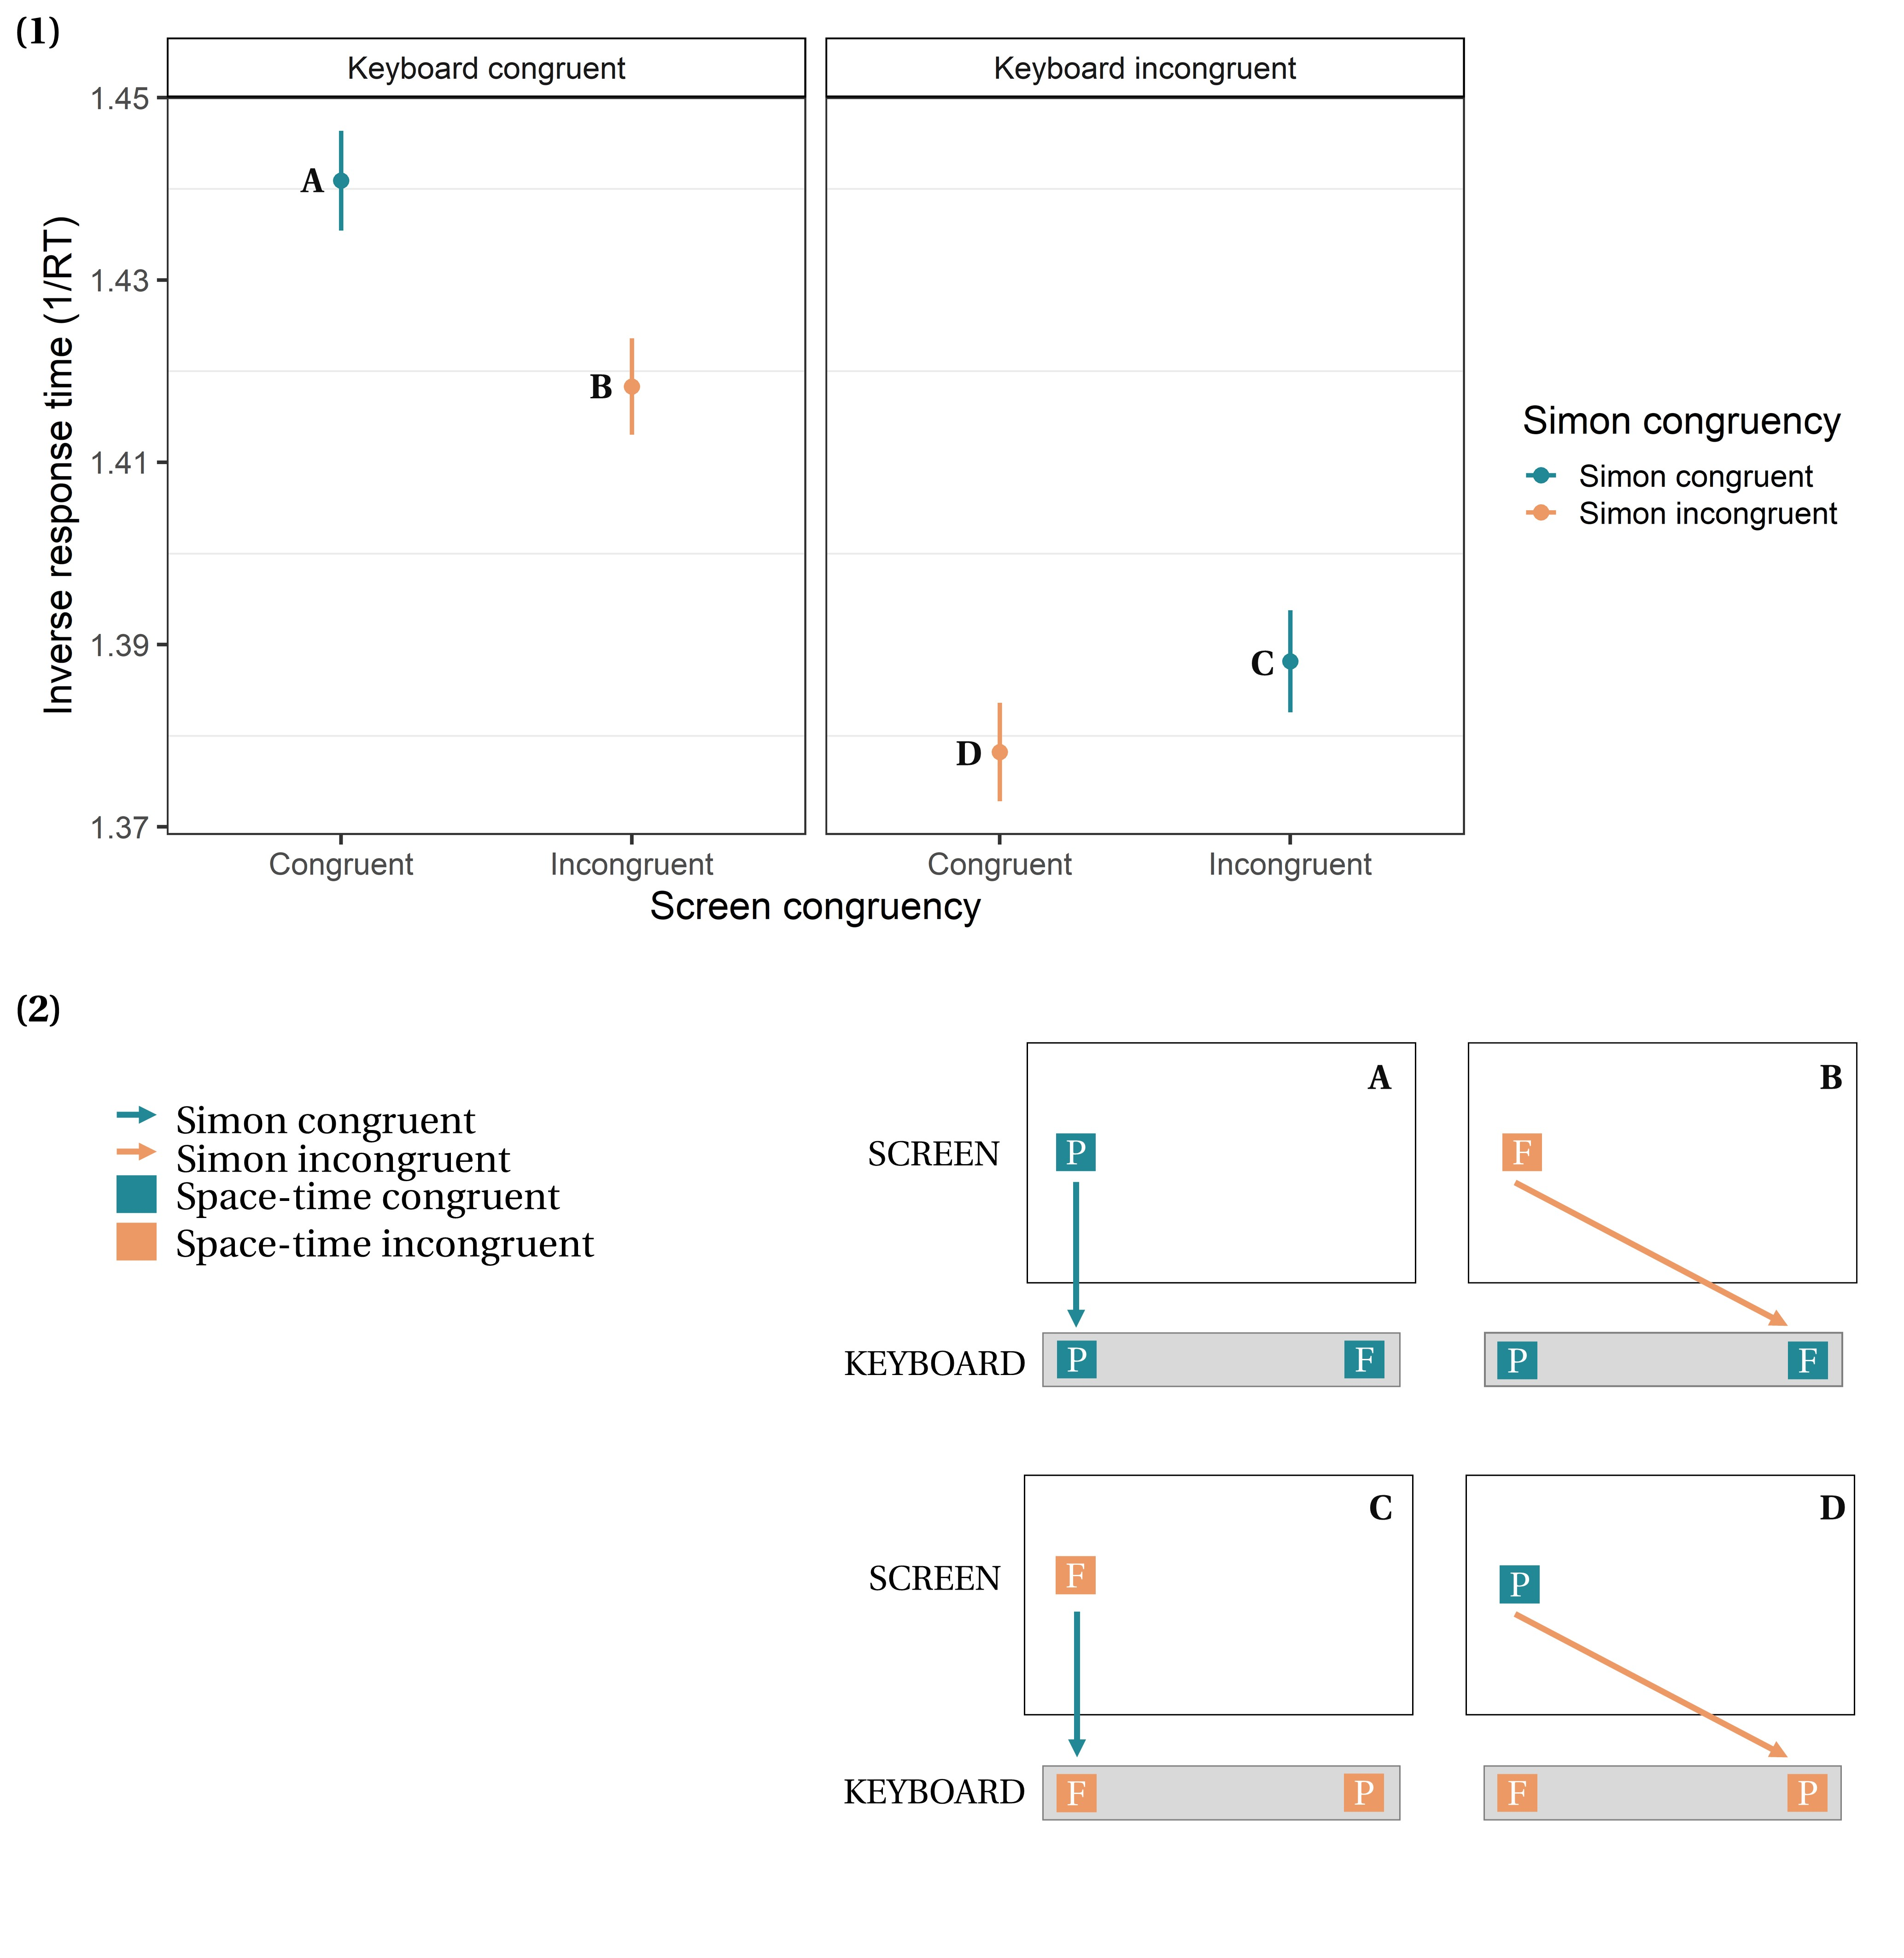
\includegraphics[width=1\linewidth]{figures/chap-5-fig3} 

}

\caption{(\textbf{1}) Inverse response latencies (i.e., higher values correspond to faster responses) for all types of congruencies, as resumed in (\textbf{2}). Error bars represent standard errors of the mean.}\label{fig:chap-5-fig3}
\end{figure}

\begin{figure}[htbp!]

{\centering 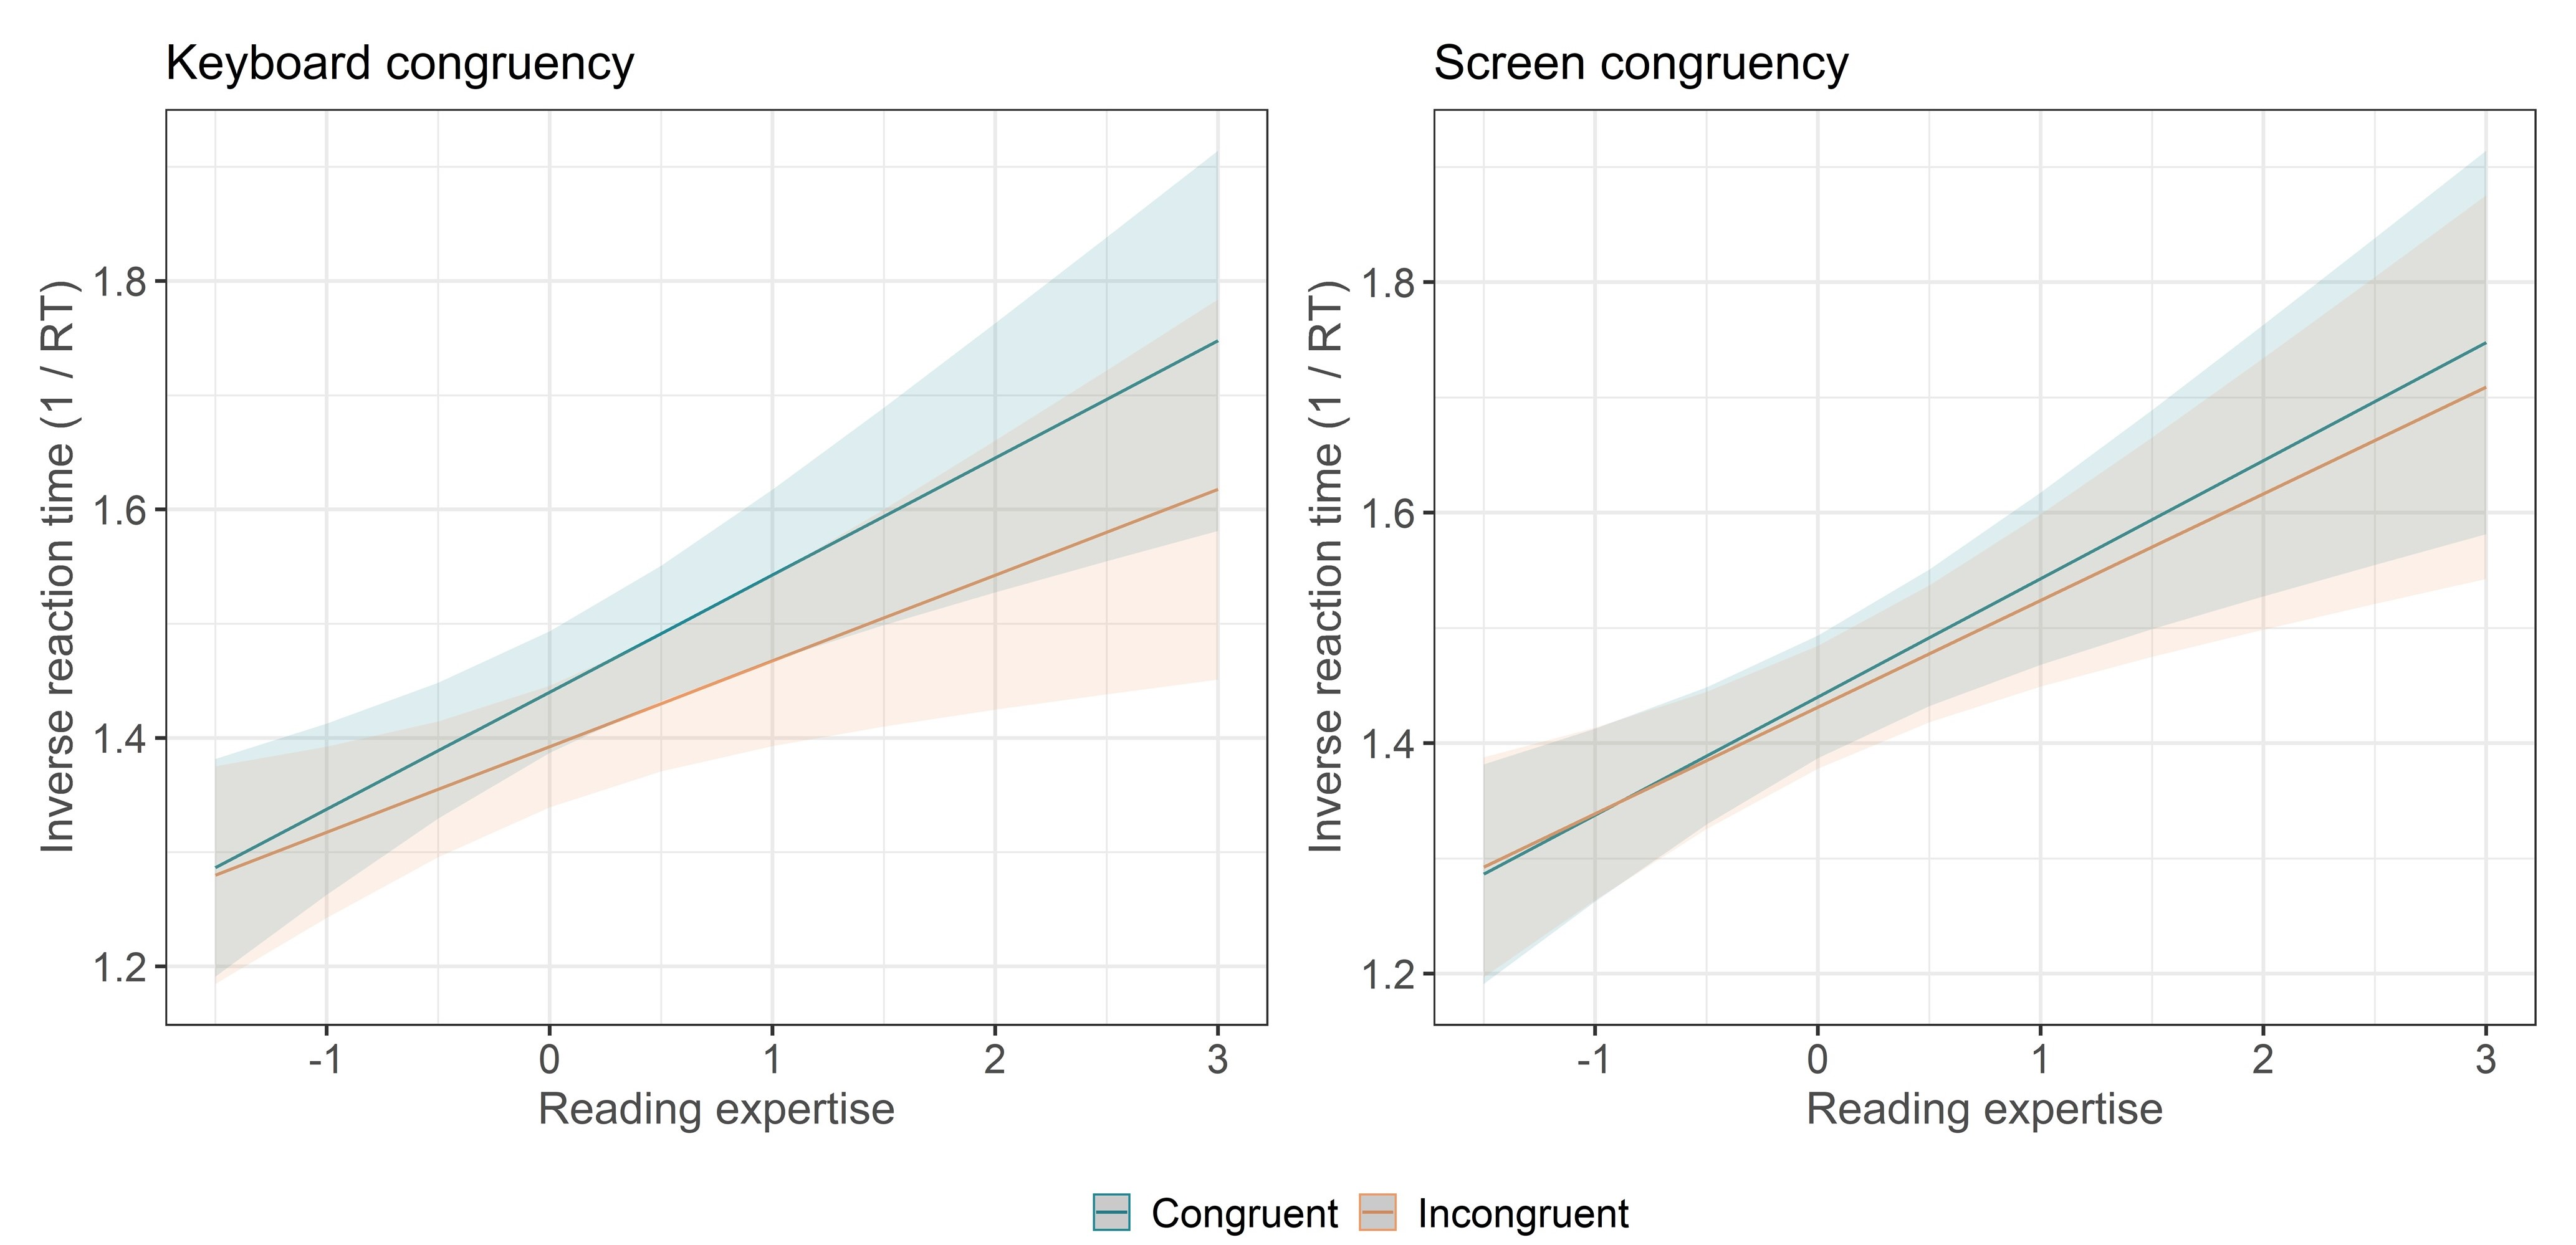
\includegraphics[width=1\linewidth]{figures/chap-5-fig4} 

}

\caption{Estimated values from the mixed models for inverse reaction times showing the interaction between reading expertise (i.e., standardised SLS score) and space-time congruencies (keyboard and screen congruency). The greater the reading experience, the greater the congruency effect, in particular in the keyboard conditions (left panel).}\label{fig:chap-5-fig4}
\end{figure}

\hypertarget{error-rate}{%
\subsection{Error rate}\label{error-rate}}

No significant effect was observed for error rate. Note that error rate was low (2.46\%).

\hypertarget{discussion-4}{%
\section{Discussion}\label{discussion-4}}

The present study was designed to investigate whether the space-time congruency effect in an explicit temporal task would be stronger if the congruency manifested itself in motor responses (keyboard congruency) rather than perceptual input (screen congruency). Second, on the basis of the assumption that the spatial representation of the temporal content of words and its directionality derives from the accumulation of writing and reading experience (e.g., \protect\hyperlink{ref-casasanto_spatial_2014}{Casasanto \& Bottini, 2014}; \protect\hyperlink{ref-fuhrman_mental_2007}{Fuhrman \& Boroditsky, 2007}; \protect\hyperlink{ref-pitt_reading_2016}{Pitt \& Casasanto, 2016}; \protect\hyperlink{ref-tillman_mental_2018}{Tillman et al., 2018}) we assessed whether reading expertise positively correlated with the size of the space-time congruency effect.

To this end, we combined reading expertise measures with an adapted version of the paradigm used by \protect\hyperlink{ref-santiago_time_2007}{Santiago et al.} (\protect\hyperlink{ref-santiago_time_2007}{2007}). This paradigm allowed us to manipulate two types of space-time congruency: 1) screen congruency; the congruency between the temporal content of stimuli (past vs.~future) and their spatial location on screen (left vs.~right), which is independent of motor execution, and 2) keyboard congruency; the congruency between the temporal content of stimuli (past vs.~future) and the associated key responses on the keyboard (left vs.~right), which involves motor execution. Combining lateralization of stimuli on the screen and lateralization of responses on the keyboard incidentally produced a Simon congruency condition, which was independent of the experimental manipulation of space-time congruency and was controlled for in the analyses. Several predictions were made: 1) as we replicated the same explicit temporal task used by \protect\hyperlink{ref-santiago_time_2007}{Santiago et al.} (\protect\hyperlink{ref-santiago_time_2007}{2007}), we should observe the same pattern of results, that is space-time congruency effects both for screen congruency and keyboard congruency conditions, 2) if lexical processing of the temporal content of words relies on both motor planning and spatial networks, then we should observe a stronger space-time congruency effect under the keyboard congruency condition, in which motor execution is needed, compared to the screen congruency condition (i.e., cumulative effect), 3) if this spatial representation of time derives from the directional movement executed while reading, then space-time congruency effects, but not the Simon congruency effect, should correlate positively with participants' reading expertise.

Statistical analyses revealed a classic Simon congruency effect, which was independent of the two space-time congruency effects. All other things being equal, participants were slower for trials in which target location on the screen and response location on the keyboard were opposed. Crucially, our results revealed a strong space-time congruency effect under the keyboard congruency condition. Average response times to complete the task were significantly longer when key responses contradicted the spatial organisation of time according to the MTL (i.e., left-future and right-past key responses), independently of other congruency conditions and of the order in which the congruent or incongruent response-mappings were given. As predicted, the effect of space-time keyboard congruency interacted with the level of reading expertise, with a higher level of reading expertise being associated with a stronger space-time congruency effect. Although the effect of space-time screen congruency was not significant in itself, it was nevertheless influenced by reading expertise, that is the higher the participants' level of reading expertise, the larger the size of the space-time screen congruency effect.

Importantly, the congruency effect was stronger for the keyboard congruency condition (\emph{SMD} = 0.131) as compared to screen congruency condition (\emph{SMD} = 0.025). In other words, the space-time congruency effect was stronger when it was implemented via a motor response, suggesting that motor networks are engaged when processing the temporal tense of a word. Altogether, these results indicate that the abstract temporal concepts of past and future are represented in both spatial and motor networks.

Crucially, participants' reading expertise correlated significantly with the size of the space-time congruency effect but not with the Simon effect. As Simon congruency is fully independent of the lexical content of stimuli, this dissociation considerably strengthens the hypothesis that the direction of the spatial representation of time (i.e., the MTL) may derive from the direction of movement during reading and writing experience (e.g., \protect\hyperlink{ref-casasanto_spatial_2014}{Casasanto \& Bottini, 2014}; \protect\hyperlink{ref-fuhrman_mental_2007}{Fuhrman \& Boroditsky, 2007}; \protect\hyperlink{ref-pitt_reading_2016}{Pitt \& Casasanto, 2016}; \protect\hyperlink{ref-tillman_mental_2018}{Tillman et al., 2018}). Furthermore, conducting an online experiment allowed us to test a large sample of the population across a considerable age range. The final mixed model included participant age as a predictor, allowing us to estimate the effect of expertise while controlling for age. Interestingly, controlling for the effect of age did not modulate the effect of reading expertise and its interaction with space-time congruency effects. This suggests that the driving force behind this correlation is specific to reading experience rather than general life experience (chronological age).

Overall, these results replicate previous findings (\protect\hyperlink{ref-grasso_as_2021}{Grasso, Ziegler, Mirault, et al., 2021}; \protect\hyperlink{ref-grasso_eye_2021}{Grasso, Ziegler, Coull, et al., 2021}; \protect\hyperlink{ref-sell_processing_2011}{Sell \& Kaschak, 2011}) and reinforce the hypothesis that the lexical processing of temporal stimuli is underpinned by motor networks, in addition to spatial brain structures. The significant interaction between reading expertise and space-time congruency effects accounts for the correlation between people's cultural habits (i.e., direction of eye movements while reading) and their tendency to organize time spatially on a left-to-right mental timeline. This result is in line with the claim that the use of spatial and motor networks for the representation of time results from reading and writing experience that creates an association between the movement of the eyes and hands rightwards or leftwards through space and the chronological order in which the left and right sides of space are experienced (e.g., Casasanto \& Bottini, 2014b).

As for the neural mechanisms that associate sensorimotor and spatial networks to the semantic representation of time, the neural reuse model (e.g., \protect\hyperlink{ref-garagnani_neuroanatomically_2008}{Garagnani et al., 2008}; \protect\hyperlink{ref-pulvermuller_neural_2018}{Pulvermüller, 2018a}) provides an interesting explanation. This model uses basic neurobiological insights about the formation of neural networks such as Hebbian learning -- and, in particular, correlational learning -- to explain how a set of sensory and motor neurons could be functionally involved in semantic processing. In short, the correlated patterns of neural activity that are present whenever a word or concept is experienced leads to the formation of strongly interconnected sets of cells distributed over the brain called action-perception circuits (APC). Regarding the abstract concept of time, it could be hypothesized that repeated experience of movements that start at one point in space and end later in time at another point associate spatial and temporal information together via correlated neural mechanisms. Repeated correlational patterns would ultimately constitute an APC consisting of, among other things, sensorimotor and spatial networks that would be automatically activated during the processing of the concept of time.

To conclude, we would like to cite \protect\hyperlink{ref-buonomano_your_2017}{Buonomano} (\protect\hyperlink{ref-buonomano_your_2017}{2017}): ``The nervous system of animals evolved sophisticated ways to represent spatial coordinates, such as up and down, left and right, before it developed the ability to explicitly represent the temporal continuum of past, present and future. This line of reasoning is consistent with the theory that our ability to grasp the concept of time was coopted from the neural circuits that evolved to navigate, represent and understand space'' (Buonomano, 2017, p.~182).

\newpage

\begin{vplace}[1]

\begin{summary}{Résumé du Chapitre\getcurrentref{chapter}}{\chaptercolor}

Comment l’individu acquière une représentation porteuse de sens pour des mots qui désignent un concept aussi abstrait que celui de temps ? Tout au long de ce manuscrit, nous avons étudié les conditions d'émergence d’effets de congruence spatio-temporelle, qui se traduisent par des temps de réponses plus rapides lorsque le contenu temporel de mots à traiter sont congruents avec l'organisation spatiale de la ligne mentale temporelle (i.e., passé à gauche et futur à droite). L’étude décrite dans ce dernier chapitre expérimental examinait deux questions : i) celle de la contribution respective des caractéristiques visuelles et motrices à l'effet de congruence spatio-temporelle, ii) et celle du rôle de l'expertise de la lecture dans l'effet de congruence spatio-temporelle. À cette fin, nous avons comparé deux conditions de congruence spatio-temporelle. Dans la première, la situation d’incongruence spatiale était générée par l'emplacement des réponses sur le clavier, tandis que dans la seconde l'incongruence spatiale était générée par l'emplacement des stimuli sur l'écran. Les résultats ont montré des effets de congruence spatio-temporelle plus forts lorsque l’incongruence spatio-temporelle était générée par le mouvement au clavier. Le deuxième résultat intéressant ici est que l'expertise en lecture, telle que mesurée par un test de lecture standardisé, prédisait la taille des effets de congruence spatio-temporelle. Dans l'ensemble, ces résultats corroborent l’hypothèse selon laquelle la représentation spatiale du temps prendait racine dans des mouvements dirigés dans l'espace, comme la lecture ou l'écriture. L’ensemble des données présentées dans ces trois chapitres expérimentaux sera discuté dans le prochain chapitre.  

\end{summary}

\end{vplace}

\hypertarget{part-discussion-et-conclusions}{%
\part{Discussion et conclusions}\label{part-discussion-et-conclusions}}

\changechaptercolor{hokusai6}

\hypertarget{chap6}{%
\chapter{Discussion et perspectives}\label{chap6}}

\epigraph{"For even if it should appear that the universe of ideas cannot be deduced from experience by logical means, but is, in a sense, a creation of the human mind, without which no science is possible, nevertheless this universe of ideas is just a little independent of the nature of our experiences as clothes are of the form of the human body. This is particularly true of our concepts of time and space"} {Einstein, A. (1922)}

\initial{Q}uels sont les mécanismes qui sous-tendent l'acquisition et la représentation des concepts abstraits temporels ? Comme discuté dans le chapitre \ref{chap1}, la question des mécanismes d'ancrage d'un concept dépourvu de caractéristiques physiques -perceptives et tangibles- est au cœur de vifs débats théoriques. Si l'implication des régions corticales sensorimotrices dès les étapes précoces du traitement linguistique de concepts concrets (e.g., \emph{cuillère}) est aujourd'hui établie dans la littérature, leurs rôles fonctionnels pour la représentation, et par conséquent le traitement, des concepts abstraits sont encore débattus. Ces dernières décennies, de nombreuses recherches ont convergé vers la proposition que les concepts abstraits temporels contiendraient une composante spatiale essentielle. À partir d'une analyse des données disponibles dans la littérature, et de propositions théoriques comme celles de réutilisation neuronale et d'apprentissage par corrélation associative, nous avons proposé une voie plus directe pour appréhender l'ancrage des concepts abstraits temporels. En effet, nous avons proposé que les concepts abstraits temporels pourraient être ancrés directement dans l'expérience sensorimotrice (e.g., dans les propriétés temporelles de l'exécution du mouvement, se décomposant en séquences de changements d'états ordonnés en avant/passé et après/futur). Dans les prochaines sections, nous présenterons un résumé des résultats obtenus, que nous discuterons à la lumière de leurs apports théoriques, mais aussi de leurs limites, et des nouvelles questions qu'ils suscitent.

\hypertarget{synthuxe8se-des-ruxe9sultats}{%
\section{Synthèse des résultats}\label{synthuxe8se-des-ruxe9sultats}}

Dans la partie théorique, nous avons développé l'hypothèse selon laquelle les concepts abstraits temporels pourraient s'ancrer directement dans l'expérience sensorimotrice en réutilisant les réseaux moteurs en charge des mouvements d'écriture et de lecture (cf.~section \ref{ancrage}). Comme l'écriture et la lecture se caractérisent par des mouvements répétés et dirigés spatialement (e.g., de la gauche vers la droite), la représentation du concept de temps contiendrait des informations spatiales organisées horizontalement (e.g., de gauche à droite), pouvant alors rendre compte des multiples observations d'une représentation spatiale du temps en une MTL. Si le concept de temps prend racine dans le mouvement, alors nous devrions observer la participation fonctionnelle, rapide et automatique, des structures corticales responsables de la planification motrice lors du traitement des concepts abstraits temporels, et devrait se manifester au niveau comportemental (sous la forme d'effets de congruence spatio-temporelle). Pour tester ces prédictions, nous avons étudié les conditions d'émergence d'effets de congruence spatio-temporelle en manipulant l'amplitude et la localisation des réponses motrices (i.e., dynamiques vs.~statiques), le type d'effecteur utilisé pour répondre (i.e., mouvements de la main vs.~mouvements oculaires), ainsi que le caractère temporel \emph{implicite} ou \emph{explicite} des paradigmes expérimentaux.

Le premier chapitre expérimental (chapitre \ref{chap3}) portait spécifiquement sur la question du rôle fonctionnel et automatique des régions motrices pour le traitement lexical de mots désignant des concepts temporels (i.e., verbes conjugués au passé ou au futur). Nous avons mis en place trois expériences utilisant une tâche de décision lexicale dans laquelle le jugement des participant·e·s ne porte pas sur la dimension temporelle des stimuli. Cette manipulation a été induite afin de tester l'hypothèse selon laquelle le traitement de mots isolés comprenant des informations grammaticales temporelles (i.e., verbes conjugués au passé ou au futur) activerait automatiquement des structures corticales motrices et spatiales, et par conséquent, se traduirait par des effets de congruence mesurables lors du traitement lexical et de l'exécution de mouvements dirigés sur l'axe horizontal gauche-droit. Pour tester le rôle du mouvement, les réponses des participant·e·s impliquaient soit des réponses dynamiques (i.e., mouvements dirigés horizontalement vers l'espace gauche ou vers l'espace droit) soit des réponses statiques (i.e., appui des touches gauche et droite d'un clavier). Les résultats de ces trois études ont montré des effets de congruence spatio-temporelle uniquement dans les conditions de réponses dynamiques (i.e., spatialement dirigées) mais pas dans les conditions de réponses statiques (i.e., pression touche), et uniquement pour les verbes (et non les pseudo-verbes).

Nous avons interprété ces résultats en faveur d'un rôle clé du mouvement dirigé dans l'espace pour l'émergence de l'effet de congruence spatio-temporelle. Comme l'attention des participant·e·s ne portait pas explicitement sur le contenu temporel des stimuli (tâche temporelle implicite) et que le niveau de complexité de la tâche était faible, l'émergence d'effets de congruence spatio-temporelle semble corroborer la prédiction d'une activation automatique des régions corticales en charge de la planification du mouvement lors du traitement lexical de mots liés aux concepts temporels. Ces résultats contrastent avec ceux précédemment observés utilisant des tâches temporelles implicites, mais également avec les conclusions de la méta-analyse de \protect\hyperlink{ref-von_sobbe_space-time_2019}{von Sobbe et al.} (\protect\hyperlink{ref-von_sobbe_space-time_2019}{2019}). Rappelons que, comme discuté dans la section \ref{axes}, l'absence d'effet de congruence spatio-temporelle mesurable lors de tâches temporelles implicites (avec réponses motrices statiques) avait rendu peu plausible l'hypothèse d'une implication automatique de régions corticales \emph{spatiales} pour le traitement des concepts abstraits temporels. Notons qu'il existe une différence cruciale entre ces études et les nôtres : l'utilisation de réponses dynamiques (i.e., spatialement dirigées). Pour cette raison, nous proposons que l'effet de congruence spatio-temporelle est sous-tendu par l'activation automatique de structures corticales dédiées à la planification motrice, plutôt que des structures corticales codant la position spatiale des mains de réponses (statiques), ou des stimuli sur l'écran. Enfin, comme discuté dans le chapitre \ref{chap2}, \protect\hyperlink{ref-barsalou_language_2008}{Barsalou et al.} (\protect\hyperlink{ref-barsalou_language_2008}{2008}) ont proposé que les concepts abstraits seraient mieux appréhendés dans leur contexte d'apparition. À l'appui de cette proposition, nous avons proposé que l'émergence d'effets de congruence observables uniquement dans les conditions de réponses dynamiques (i.e., spatialement dirigées), puisse s'expliquer par les similarités entre le contexte expérimental (nécessitant des réponses dynamiques) et le contexte d'ancrage du concept de temps, nécessitant des mouvements dirigés depuis et vers des coordonnées de l'espace (e.g., pendant l'écriture et la lecture).

En effet, nous avons interprété ces résultats à la lumière des données interculturelles en suggérant qu'ils corroboraient l'hypothèse d'un ancrage dans les mouvements répétés de lecture et d'écriture (allant de gauche à droite, e.g., \protect\hyperlink{ref-fuhrman_mental_2007}{Fuhrman \& Boroditsky, 2007}). Notons cependant que nos protocoles ne permettaient pas un test direct de cette hypothèse. En effet, si nos résultats étayent le rôle de structures corticales motrices pour la représentation du concept de temps, ils ne fournissent aucune preuve directe, ni sur le rôle de l'écriture et de la lecture, ni sur le rôle spécifique de structures corticales en charge de la planification motrice (parmi les structures motrices), pour la représentation des concepts temporels.

Dans l'expérience 4 (chapitre \ref{chap4}), nous avons utilisé un paradigme d'analyse des mouvements oculaires (i.e., occulométrie) pour tester la généralité de nos effets à d'autres modalités de réponses. Précisons également que jusqu'ici, l'ensemble des études faisant état d'effets de congruence spatio-temporelle pour le traitement de mots liés au temps avaient utilisé uniquement des réponses manuelles. Si la représentation du concept de temps contient des informations spatiales qui dérivent de l'activité d'écriture et de lecture, alors les informations spatiales réutilisées pour la représentation temporelle (i.e., organisées en une MTL) ne devraient pas seulement concerner la main (impliquée pendant l'écriture), mais devraient se généraliser aux mouvements oculaires (impliqués pendant la lecture). De la même façon, comme la planification de mouvements implique la traduction d'informations spatiales en commandes motrices, répliquer des effets de congruence spatio-temporelle avec les mouvements oculaires fournirait des pistes concernant une possible implication des réseaux généraux de planification motrice, et dont le cadre de référence spatiale serait centré sur le corps entier (e.g., \protect\hyperlink{ref-rosenbaum_human_1991}{Rosenbaum, 1991}; \protect\hyperlink{ref-schmidt_motor_2019}{Schmidt et al., 2019}), plutôt que centré sur l'effecteur de la main. Pour examiner ces prédictions, nous avons mis en place une expérience où les réponses de la tâche de décision lexicale se faisaient par des mouvements oculaires (saccade balistique) vers l'espace gauche ou vers l'espace droit de l'écran où étaient présentés les stimuli. L'analyse des résultats réplique les effets de congruence spatio-temporelle obtenus dans le chapitre \ref{chap3} avec les réponses manuelles sur deux composantes motrices de la saccade réponse, à savoir le temps d'initiation, qui est analogue au temps d'initiation de la réponse motrice manuelle, et l'amplitude, qui informe plus directement sur les processus de planification motrice de la saccade. De nouveau, ces résultats obtenus lors d'une tâche de décision lexicale (tâche temporelle implicite) sont consistants avec l'hypothèse d'une participation fonctionnelle, rapide et automatique, de régions corticales en charge de la planification motrice. Le fait de répliquer ces effets avec les mouvements oculaires suggère que les informations spatiales associées au concept de temps sont centrées sur le corps entier (et non sur la localisation de l'effecteur dans l'espace), et font référence à l'espace extra-personnel. Pour le dire autrement, ce cadre de référence spatiale, dans lequel le mouvement se produit (spatialement de gauche à droite) serait codé indépendamment de l'effecteur et serait réutilisé pour représenter le concept de temps. Enfin, ces résultats suggèrent que les informations spatiales utilisées pour représenter le temps dérivent de la répétition de mouvements directionnels culturellement dépendants, habituellement produits pendant l'écriture et la lecture (e.g., \protect\hyperlink{ref-fuhrman_mental_2007}{Fuhrman \& Boroditsky, 2007}; \protect\hyperlink{ref-oliveri_representation_2009}{Oliveri et al., 2009}).

Cependant, comme ce paradigme expérimental réplique ceux utilisés dans le chapitre \ref{chap3}, il ne permet pas non plus de tester empiriquement l'hypothèse d'un ancrage dans les mouvements d'écriture et de lecture. Dans le dernier chapitre expérimental (chapitre \ref{chap5}), nous avons examiné le rôle du mouvement et de l'expertise de la lecture dans l'effet de congruence spatio-temporelle traditionnellement observé lors de tâches de catégorisation temporelle (tâche temporelle explicite). L'étude présentée dans ce chapitre aborde deux questions théoriques non résolues. Premièrement, elle aborde la question de la contribution respective des facteurs spatiaux visuels et moteurs à l'effet de congruence spatio-temporelle lors d'une tâche temporelle explicite. Deuxièmement, elle étudie le rôle de l'expertise en lecture dans l'émergence de l'effet de congruence spatio-temporelle. Nos résultats répliquent les effets de congruence spatio-temporelle précédemment obtenus lors de tâches temporelles explicites avec réponses motrices statiques (i.e., pression des touches d'un clavier). De manière intéressante, l'effet était plus marqué lorsque l'incongruence spatio-temporelle était induite par la localisation des réponses motrices (vs.~localisation des stimuli sur l'écran), et d'autant plus fort avec une plus grande expertise de lecture des participant·e·s. Cette dernière étude apporte un soutien empirique plus direct en faveur de l'influence des mouvements répétés d'écriture et de lecture pour la représentation spatiale du concept de temps, et a été interprété à la lumière des mécanismes proposés par le modèle des APC (discutés dans la section \ref{apc}). Notamment, ces résultats corroborent le postulat selon lequel le concept de temps serait directement ancré dans l'expérience répétée des mouvements qui débutent en un point de l'espace-temps et se terminent plus tard en un autre point. Ces résultats sont compatibles avec l'idée que les informations spatiales et temporelles se chevauchent par le biais de mécanismes d'apprentissage par corrélation associative.

Pour résumer, les résultats décrits dans ces trois chapitres apportent des arguments empiriques supplémentaires en faveur d'un rôle clé des régions corticales motrices pour l'émergence d'effets de congruence spatio-temporelle lors de tâches temporelles implicites et explicites. De tels effets semblent intervenir automatiquement et uniquement lorsque les stimuli sont des mots existants (vs.~des non-mots), ce qui suggère que l'implication de ces régions corticales participe à la construction lexicale du contenu temporel des mots. De manière générale, ces résultats sont cohérents avec la proposition d'un ancrage direct du concept de temps dans l'expérience sensorimotrice. À la lumière des mécanismes proposés par les APC, nous proposons que le concept de temps pourrait être ancré dans un réseau distribué composé, entre autres, de structures corticales sensorimotrices (en charge de la planification du mouvement) et spatiales qui seraient rapidement et automatiquement activées lors de la présentation de mots faisant référence au concept de temps. Ces résultats ont de nombreuses implications théoriques que nous proposons de discuter en plusieurs sections. La première partie de ces discussions reprendra celles faites dans les chapitres expérimentaux plus en détail, et proposera une (ré)analyse des données disponibles. Ensuite, deux sections seront dédiées aux interprétations des résultats à la lumière des théories incarnées du langage et des connaissances disponibles sur la cognition temporelle.

\hypertarget{implications-thuxe9oriques-des-ruxe9sultats}{%
\section{Implications théoriques des résultats}\label{implications-thuxe9oriques-des-ruxe9sultats}}

\hypertarget{discussion-des-ruxe9sultats-nouvelle-lecture-des-donnuxe9es-issues-de-la-littuxe9rature}{%
\subsection{Discussion des résultats : nouvelle lecture des données issues de la littérature}\label{discussion-des-ruxe9sultats-nouvelle-lecture-des-donnuxe9es-issues-de-la-littuxe9rature}}

Quel est le rôle des régions corticales \emph{spatiales} pour la représentation des concepts abstraits temporels ? Les résultats présentés dans les chapitres expérimentaux sont consistants avec les précédentes observations faisant état de chevauchements corticaux entre le domaine spatial et le domaine temporel (pour revues voir \protect\hyperlink{ref-bender_mapping_2014}{Bender \& Beller, 2014}; \protect\hyperlink{ref-bonato_when_2012}{Bonato et al., 2012}; \protect\hyperlink{ref-lewandowska-tomaszczyk_mental_2016}{Eikmeier et al., 2016}). Cependant, nos résultats fournissent de nouvelles pistes explicatives concernant ces chevauchements et des éléments de réponse pertinents aux questions précédemment non résolues.

La première implication théorique que nous aborderons est celle du rôle des régions corticales motrices - et notamment de planification motrice - en plus des régions corticales spatiales, pour la représentation des concepts temporels. Comme discuté dans le chapitre \ref{chap2}, de nombreuses études ont déjà rapporté des effets d'interactions entre production de mouvements et traitement des concepts abstraits temporels. Par exemple, l'analyse des gestes spontanés produits pendant le discours oral montre une organisation fréquente des mouvements sur l'axe gauche-droit, ce qui correspond à l'organisation spatiale du temps (\protect\hyperlink{ref-casasanto_hands_2012}{Casasanto \& Jasmin, 2012}). Autrement dit, si vous devez expliquer la différence entre les mots « hier » et « demain », il est fort probable que vous réalisiez des gestes vers votre espace gauche pour le passé et des gestes vers votre espace droit pour le futur. Selon \protect\hyperlink{ref-cooperrider_how_2016}{Cooperrider \& Núñez} (\protect\hyperlink{ref-cooperrider_how_2016}{2016}), ces mouvements spontanés révèlent votre façon de conceptualiser spatialement le temps. Par ailleurs, demander à des participant·e·s d'imaginer que le temps avance vers eux, ou que ce sont eux qui avancent dans le temps, induit des changements mesurables dans leur façon de conceptualiser le passé et le futur (\protect\hyperlink{ref-boroditsky_roles_2002}{Boroditsky \& Ramscar, 2002}). Enfin, \protect\hyperlink{ref-jamalian_gestures_2012}{Jamalian \& Tversky} (\protect\hyperlink{ref-jamalian_gestures_2012}{2012}) ont montré que réaliser des gestes qui variaient dans leur orientation spatiale pendant la présentation de contenu linguistique invariant suffisait à influencer l'organisation spatiale du temps chez les participant·e·s. Enfin, l'analyse des mouvements oculaires sur un écran vide lors de l'encodage et la récupération de mots désignant des concepts temporels passé et futur ont montré une tendance chez les participant·e·s à placer leur regard dans l'espace gauche de l'écran pour les mots désignant le passé et inversement pour les mots désignant le futur (\protect\hyperlink{ref-hartmann_eye_2014-1}{Hartmann et al., 2014}; \protect\hyperlink{ref-martarelli_time_2017}{Martarelli et al., 2017}). Ces résultats impliquent non seulement des notions de localisation spatiale mais aussi de mouvements pour la représentation des concepts temporels. Bien que les théories de la métaphore conceptuelle aient identifié l'importance des mouvements spatialement dirigés pour la conceptualisation du temps, notons cependant que le rôle du mouvement est ici considéré comme de second ordre, décrit comme le reflet de l'organisation \emph{spatiale} du temps. En effet, rappelons que les théories conceptuelles soutiennent que la cognition temporelle, et par conséquent le concept de temps, serait intrinsèquement de nature spatiale (e.g., \protect\hyperlink{ref-boroditsky_metaphoric_2000}{Boroditsky, 2000}; \protect\hyperlink{ref-lakoff_philosophy_1999}{Lakoff \& Johnson, 1999}). Ce postulat implique une dépendance de l'espace pour la représentation du temps. Si nous rejoignons les théories de la métaphore conceptuelle sur le principe d'une relation étroite entre l'espace et le temps, nous suggérons cependant une distinction entre domaine spatial et domaine temporel et proposons un rôle de premier ordre du mouvement pour l'ancrage des concepts abstraits temporels. En effet, à la lumière des discussions engagées dans la section \ref{lim-con}, nous avons proposé que le temps ne serait pas intrinsèquement de nature spatiale (voir aussi \protect\hyperlink{ref-kranjec_are_2010}{Kranjec \& Chatterjee, 2010}), même si de nombreux chevauchements inter-domaines ont été établis. Sur ce point, les résultats que nous avons obtenus rejoignent davantage les propositions faites par la théorie ATOM (\protect\hyperlink{ref-bueti_parietal_2009}{Bueti \& Walsh, 2009}; \protect\hyperlink{ref-walsh_theory_2003}{Walsh, 2003}). Pour rappel, la théorie ATOM propose un système commun pour le traitement des ordres de grandeur, comme l'espace et le temps,\footnote{Dans le cadre de la théorie ATOM, le temps fait principalement référence à la durée temporelle.} pour la coordination de l'action dans l'environnement. Dans ce cadre, le temps et l'espace seraient souvent confondus parce qu'ils interviennent tous les deux pour la planification de l'action. Des conclusions similaires ont été proposées par \protect\hyperlink{ref-sell_processing_2011}{Sell \& Kaschak} (\protect\hyperlink{ref-sell_processing_2011}{2011}; répliquée par \protect\hyperlink{ref-scheifele_replication_2018}{Scheifele et al., 2018}). En effet, \protect\hyperlink{ref-sell_processing_2011}{Sell \& Kaschak} (\protect\hyperlink{ref-sell_processing_2011}{2011}) ont proposé que l'effet de congruence spatio-temporelle rapporté sur l'axe avant-arrière dans une condition avec mouvements dynamiques (i.e., spatialement dirigés) dans une tâche temporelle implicite traduirait l'implication de régions pariétales impliquées dans la planification motrice, et par conséquent du traitement du concept abstrait de temps. Selon nous, ces propositions sont consistantes avec les mécanismes d'apprentissage par corrélation associative et pourraient expliquer comment le concept de temps pourrait être directement ancré dans l'expérience temporelle inhérente au mouvement, et comment le mouvement pourrait être l'expérience sensorimotrice qui associe l'espace et le temps. Des discussions plus approfondies sur ces points seront proposées dans les prochaines sections.

Un autre point de discussion important soulevé par nos résultats est la part fonctionnelle des régions corticales motrices pour le traitement des concepts abstraits temporels. Rappelons brièvement que si les effets de congruence spatio-temporelle paraissent robustes pour des tâches temporelles explicites (e.g., tâche de catégorisation passé et futur, \protect\hyperlink{ref-aguirre_potential_2017}{Aguirre \& Santiago, 2017}; \protect\hyperlink{ref-casasanto_spatial_2014}{Casasanto \& Bottini, 2014}; \protect\hyperlink{ref-de_la_vega_mental_2016}{de la Vega et al., 2016}), ces effets sont considérablement réduits, voir absents, pour des tâches temporelles implicites (e.g., tâche de jugement de grammaticalité ou de décision lexicale, voir méta-analyse de \protect\hyperlink{ref-von_sobbe_space-time_2019}{von Sobbe et al., 2019}). Pour ces auteur·e·s, ces inconsistances de résultats semblaient incompatibles avec la proposition d'une activation automatique des informations \emph{spatiales} dans le traitement des concepts abstraits temporels.\footnote{Si l'activation des structures spatiales était automatique lors du traitement de stimuli temporels, alors l'effet de congruence spatio-temporelle devrait émerger peu importe le type de tâche réalisée par les participant·e·s.} \protect\hyperlink{ref-von_sobbe_space-time_2019}{von Sobbe et al.} (\protect\hyperlink{ref-von_sobbe_space-time_2019}{2019}) avaient suggéré que les effets de congruence spatio-temporelle pourraient être mieux expliqués par un effet de facilitation d'accès en mémoire lorsque l'attention des participant·e·s porte explicitement sur le contenu temporel des stimuli (i.e., tâche temporelle explicite). Comme expliqué précédemment, nous avons adopté un autre point de vue pour rendre compte de ces inconsistances, en mettant en avant le rôle du mouvement dynamique (i.e., spatialement dirigé). Les expériences décrites dans les chapitres \ref{chap3} et \ref{chap4} ont mis en évidence des effets de congruence spatio-temporelle dans des tâches de décision lexicales. Comme l'attention des participant·e·s ne portait pas sur le contenu temporel des stimuli (expériences 1 à 4), ces résultats rejoignent ceux obtenus par \protect\hyperlink{ref-sell_processing_2011}{Sell \& Kaschak} (\protect\hyperlink{ref-sell_processing_2011}{2011}) sur l'axe avant-arrière et suggèrent une participation automatique des structures corticales motrices pour le traitement lexical de mots désignant des concepts temporels. De même, comme ces effets de congruences n'interférent qu'avec le traitement de mots existants (i.e., pour les mots et non pour les non-mots), cela étaye davantage la participation fonctionnelle de ces structures motrices.

Reprenons le raisonnement développé dans le chapitre \ref{chap1}. Si une fonction \texttt{A} est sous-tendue par un réseau de neurones déjà en cours d'utilisation pour une fonction \texttt{B}, alors on devrait observer des effets d'interférences mesurables entre \texttt{A} et \texttt{B} (mesurables ici par des ralentissements de temps de réponse). Pour ces raisons, nous avons proposé que l'effet de congruence spatio-temporelle émerge car, dans les conditions d'incongruence, les mouvements de réponse gauche ou droit activent des réseaux de planification de mouvements allant dans une direction de l'espace incompatible avec l'information spatiale qui sous-tend la représentation des concepts temporels (en comparaison aux conditions avec réponses motrices statiques). Par conséquent, il est possible que l'utilisation de réponses motrices statiques (i.e., pression des touches du clavier, e.g., \protect\hyperlink{ref-maienborn_we_2015}{Maienborn et al., 2015}; \protect\hyperlink{ref-ulrich_leftright_2010}{Ulrich \& Maienborn, 2010}) n'ait pas fourni les conditions nécessaires à l'émergence d'effet de congruence spatio-temporelle mesurable dans une tâche où l'attention des participant·e·s n'était pas focalisée sur le contenu temporel des stimuli.

Par ailleurs, si les mouvements dynamiques (i.e., spatialement dirigés) semblent déterminants pour l'émergence d'effets de congruence spatio-temporelle dans des tâches temporelles implicites, qu'en est-il des tâches temporelles explicites où les réponses motrices statiques semblent suffisantes pour l'émergence d'effets mesurables ? Comme la différence principale entre ces deux types de tâches est l'attention fournie par les participant·e·s sur le contenu temporel des stimuli, nous pensons que les fonctions attentionnelles peuvent fournir une piste de réflexion pertinente.

Pour rappel, nous avons évoqué dans la section \ref{axes} les observations cliniques où des patients souffrant de négligence spatiale unilatérale (consécutive à une lésion pariétale) présentent des difficultés à la fois pour le traitement de l'hémi-espace gauche et pour le traitement des évènements passés (e.g., \protect\hyperlink{ref-saj_patients_2014}{Saj et al., 2014}). De manière cruciale, ce tableau clinique se caractérise (entre autres choses) par une altération importante des fonctions attentionnelles visuospatiales (e.g., \protect\hyperlink{ref-mesulam_cortical_1981}{Mesulam, 1981}; \protect\hyperlink{ref-posner_effects_1984}{Posner et al., 1984}). De concert avec les propositions de \protect\hyperlink{ref-sell_processing_2011}{Sell \& Kaschak} (\protect\hyperlink{ref-sell_processing_2011}{2011}) décrites précédemment concernant le rôle des régions corticales pariétales pour la représentation des concepts abstraits temporels, nous pouvons nous demander si les effets de congruence spatio-temporelle mesurés dans des tâches temporelles explicites émergent justement parce qu'elles sollicitent un traitement attentionnel sur le contenu temporel de stimuli associés à différentes coordonnées spatiales. Pour le dire autrement, il se pourrait que cet engagement attentionnel sur le contenu temporel des stimuli suffise à provoquer des effets de congruence spatio-temporelle mesurables parce que ces réseaux attentionnels sont impliqués dans le traitement des concepts temporels. Dans les tâches implicites, l'attention volontaire sur le contenu temporel des stimuli est absente. Si le traitement conceptuel du concept de temps engage des structures corticales motrices, il est plausible que des réponses statiques ne suffisent pas à générer des effets de congruence mesurables (s'ils existent). Rappelons que nous avons proposé dans l'expérience rapportée au chapitre \ref{chap5}, que si le rôle des régions motrices se trouvait aussi important pour une tâche temporelle explicite, alors nous devrions observer des effets cumulatifs, à savoir des effets de congruence spatio-temporelle plus marqués dans les conditions où l'incongruence est déterminée par la localisation des réponses motrices (statiques au clavier), en comparaison à une condition où l'incongruence est déterminée par la localisation spatiale du stimulus sur l'écran (i.e., visuelle). Bien que nos résultats semblent consistants avec cette prédiction, ces interprétations sont néanmoins à prendre avec précaution. En effet, rappelons que les effets de congruence sont mesurés par des différences de temps de réponses. Si nous avons contrebalancé la localisation de la réponse (i.e., gauche droite) associée au temps du stimuli (i.e, passé ou futur), et que nous avons comparé des différences de temps de réponse pour des stimuli localisés à gauche ou à droite de l'écran indépendamment de la localisation gauche droite des réponses au clavier, l'exécution motrice n'est jamais purement contrôlée pour la condition d'incongruence à l'écran (puisque mesurée par l'exécution motrice). Une manière plus directe de tester ces effets cumulatifs dans une tâche temporelle \emph{explicite} serait de comparer des tailles d'effets de congruence spatio-temporelle entre des conditions avec réponses motrices dynamiques (i.e., spatialement dirigées) et des conditions sans réponses motrices dynamiques. Si de tels effets cumulatifs existent (entre l'attention spatiale et la planification de mouvements dynamiques et spatialement dirigés), alors nous devrions observer des tailles d'effets plus importantes dans les conditions avec mouvements dynamiques, par rapport aux conditions sans mouvements dynamiques (i.e., avec réponses motrices statiques). Notons que la comparaison entre deux conditions d'incongruence spatio-temporelle n'était pas l'unique objectif de cette expérience (chapitre \ref{chap5}).

Dans la section \ref{ancrage}, nous avons discuté des données interculturelles qui suggèrent que les associations spatiales et temporelles en une MTL correspondent au sens d'écriture et de lecture des participant·e·s. Précisément, lorsque l'on teste les biais directionnels spatio-temporels chez des participant·e·s dont le système d'écriture va de la gauche vers la droite (comme la plupart des systèmes d'écritures latines), le passé se trouve associé avec l'espace gauche et le futur avec l'espace droit. Si l'on reproduit cette expérience avec des participant·e·s dont le système d'écriture va de la droite vers la gauche, comme l'hébreu ou l'arabe, ces effets sont inversés, décrivant alors une association gauche-futur et droit-passé (e.g., \protect\hyperlink{ref-bergen_writing_2012}{Bergen \& Chan Lau, 2012}; \protect\hyperlink{ref-hutchison_can_2010}{Casasanto \& Bottini, 2010}; \protect\hyperlink{ref-fuhrman_mental_2007}{Fuhrman \& Boroditsky, 2007}). Quant aux participant·e·s qui lisent et écrivent verticalement de haut en bas, comme le mandarin, les concepts abstraits temporels seraient organisés du haut vers le bas (e.g., \protect\hyperlink{ref-boroditsky_english_2011}{Boroditsky et al., 2011}; \protect\hyperlink{ref-de_sousa_generational_2012}{de Sousa, 2012}). Enfin, quelques minutes de lecture en miroir suffisent pour inverser la direction des effets de congruence spatio-temporelle (\protect\hyperlink{ref-hutchison_can_2010}{Casasanto \& Bottini, 2010}; \protect\hyperlink{ref-pitt_reading_2016}{Pitt \& Casasanto, 2016}), ce qui a été interprété en faveur d'une implication causale de l'écriture et de la lecture pour l'organisation spatiale des concepts abstraits temporels. Ces observations se sont traduites dans l'hypothèse selon laquelle la représentation spatiale du concept de temps dérive de l'accumulation d'expériences motrices répétées au cours de l'écriture et de la lecture (e.g., \protect\hyperlink{ref-casasanto_spatial_2014}{Casasanto \& Bottini, 2014}; \protect\hyperlink{ref-pitt_reading_2016}{Pitt \& Casasanto, 2016}; \protect\hyperlink{ref-tillman_mental_2018}{Tillman et al., 2018}). À l'appui de cette hypothèse, les données rapportées dans l'expérience 5 révèlent une interaction entre le niveau de lecture des participant·e·s et la taille des effets de congruence spatio-temporelle (clavier et écran) : plus le niveau d'expertise en lecture était haut, plus l'effet de congruence spatio-temporelle était marqué. Il importe cependant de noter qu'observer une interaction entre niveau de lecture et taille d'effet de congruence spatio-temporelle n'implique pas nécessairement une influence causale de l'écriture et la lecture pour la représentation du concept de temps. Une autre explication, tout aussi plausible, pourrait être que l'effet de congruence soit partiellement expliqué par la vitesse de traitement de l'information des participant·e·s. En effet, comme graphiquement représenté dans la Figure \ref{fig:chap-5-fig4}, les participant·e·s avec le plus haut niveau d'expertise en lecture sont aussi les plus rapides pour répondre. Nous avons supposé que l'effet de congruence spatio-temporelle intervenait dès les étapes précoces de la reconnaissance des mots, nous pouvons alors nous demander si l'interaction observée entre ces deux construits (i.e., le niveau d'expertise en lecture et l'effet de congruence spatio-temporelle) ne pourrait pas être expliquée plus simplement par la vitesse de traitement de l'information des participant·e·s.

Concernant le lien causal de l'expérience de l'écriture et de la lecture, nous avons discuté des données rapportées par \protect\hyperlink{ref-casasanto_spatial_2014}{Casasanto \& Bottini} (\protect\hyperlink{ref-casasanto_spatial_2014}{2014}) où ces auteur·e·s ont montré que la lecture en miroir se traduisait par l'inversion du biais directionnel de l'effet de congruence spatio-temporelle (voir aussi \protect\hyperlink{ref-pitt_reading_2016}{Pitt \& Casasanto, 2016}). Ces observations restent insuffisantes pour affirmer que l'ancrage des concepts temporels soit le produit des mouvements répétés d'écriture et de lecture. En outre, il est envisageable que d'autres expériences de la vie quotidienne, caractérisées par des mouvements répétés allant de gauche à droite, puissent sous-tendre l'apprentissage d'associations spatiales (gauche, droite) et temporelles (passé, futur). À titre d'exemple, au vu des mécanismes proposés par les APC, il se pourrait que des renforcements par apprentissage par corrélation puissent intervenir pendant l'expérience perceptive visuelle de la lecture d'histoires (où l'adulte réalise des gestes allant de gauche à droite) avant la scolarisation de l'enfant, et donc avant l'apprentissage de la lecture. Un moyen plus direct pour examiner la question du rôle de l'apprentissage de l'écriture et de la lecture serait de réaliser une étude développementale auprès d'enfants afin de déterminer le décours développemental de ces effets de congruence spatio-temporelle pour le traitement lexical de mots désignant des concepts temporels (voir par exemple \protect\hyperlink{ref-tillman_mental_2018}{Tillman et al., 2018}, \protect\hyperlink{ref-tillman_building_2016}{2016}, pour des données sur le traitement de l'ordre des évènements, hors langage).

Pour résumer, plusieurs propositions concernant les mécanismes qui sous-tendent la représentation des concepts abstraits temporels peuvent être formulées. La première est que les concepts abstraits temporels pourraient s'ancrer directement dans l'expérience temporelle qui intervient lors de l'exécution de mouvements. En ce sens, nous proposons que les chevauchements qui existent entre domaine spatial et domaine temporel n'impliquent pas nécessairement que le temps soit (intrinsèquement) de nature spatiale, et nous avons insisté sur le rôle clé du mouvement pour son ancrage. La deuxième, qui découle de la première, est que les mécanismes neuronaux qui sous-tendent la représentation et le traitement des concepts temporels pourraient réutiliser ceux de la planification motrice, en plus des régions corticales spatiales et attentionnelles. La troisième, qui mériterait davantage d'étayage empirique, est que les mouvements répétés lors de l'écriture et de la lecture pourraient constituer l'expérience sensorimotrice qui donne son cadre d'ancrage au concept de temps, et qui lie ensemble espace et temps via un apprentissage par corrélation. Dans les sections suivantes, nous discuterons des implications de ces résultats pour le traitement des concepts abstraits. Nous discuterons également de l'interprétation que nous pouvons donner à ces résultats à la lumière des connaissances disponibles sur la cognition temporelle.

\hypertarget{implications-des-ruxe9sultats-pour-le-traitement-des-concepts-abstraits}{%
\subsection{Implications des résultats pour le traitement des concepts abstraits}\label{implications-des-ruxe9sultats-pour-le-traitement-des-concepts-abstraits}}

\hypertarget{modalituxe9-de-repruxe9sentation-des-concepts-abstraits}{%
\subsubsection{Modalité de représentation des concepts abstraits}\label{modalituxe9-de-repruxe9sentation-des-concepts-abstraits}}

Quel est le rôle fonctionnel des structures corticales sensorimotrices pour le traitement conceptuel ? Autrement dit, dans quelle mesure les connaissances conceptuelles sont-elles façonnées par les expériences sensorimotrices des situations qui les accompagnent ? Enfin, comment des concepts abstraits pourraient-ils prendre racine dans un ensemble d'interactions sensorimotrices si, par définition, ils n'ont pas de référents physiques manipulables par les systèmes sensorimoteurs ? Les résultats décrits dans les chapitres expérimentaux ne permettent pas de fournir de réponses définitives à ces questions. Cependant, nous espérons que ces résultats permettent d'éclairer (modestement) les discussions engagées dans le chapitre \ref{chap1}.

Pour rappel, nous avons adopté les différentes prédictions formulées par \protect\hyperlink{ref-pulvermuller_brain_2005}{Pulvermüller} (\protect\hyperlink{ref-pulvermuller_brain_2005}{2005}) concernant le traitement de mots désignant des concepts concrets pour le traitement de mots désignant des concepts abstraits temporels (section \ref{pred}). Les résultats décrits dans ce manuscrit corroborent ces prédictions (cf.~section \ref{predictionth}), et sont consistants avec les données disponibles concernant le traitement des concepts concrets. Premièrement, les effets de congruence spatio-temporelle rapportés lors de conditions de mouvements dynamiques (i.e., spatialement dirigés) pour le traitement lexical de mots liés au temps suggèrent une activation spécifique à la modalité d'encodage du concept de temps, à savoir les structures corticales en charge de la planification de mouvements dirigés (cf.~section \ref{incarnation}). Deuxièmement, nos résultats sont cohérents avec l'hypothèse d'une activation rapide et automatique de structures corticales motrices, dans le sens où les effets de congruence spatio-temporelle ne dépendent pas de l'attention explicite des participant·e·s sur le contenu temporel des stimuli. Rappelons que si ces résultats corroborent la participation de structures corticales motrices, il ne s'agit que de mesures indirectes de cette participation pour le traitement lexical. Comme discuté précédemment, \protect\hyperlink{ref-sternberg_discovery_1969}{Sternberg} (\protect\hyperlink{ref-sternberg_discovery_1969}{1969}) a établi que les effets d'interaction entre deux facteurs manipulés impliquent une composante partagée entre les deux processus. Dans notre cas, nous proposons que les effets de congruence spatio-temporelle qui émergent dans les conditions de mouvements dynamiques (i.e., spatialement dirigés) pour le traitement de mots désignant des concepts abstraits temporels (i.e., verbes conjugués au passé ou au futur) suggèrent que le concept de temps réutilise, entre autres, des réseaux moteurs en charge de la planification motrice. Ces résultats sont également cohérents avec les données décrites concernant les concepts concrets qui montrent des activations rapides et automatiques des structures spécifiques à leurs modalités d'ancrage (e.g., \protect\hyperlink{ref-boulenger_subliminal_2008}{Boulenger et al., 2008}; \protect\hyperlink{ref-pulvermuller_brain_2005}{Pulvermüller, 2005}).

Ensemble, ces résultats fournissent des arguments en faveur d'une participation de structures corticales sensorimotrices pour le traitement lexical de mots liés aux concepts abstrait temporels, et contre le principe d'une implication seulement épiphénomènale de ces structures. Le fait d'observer des effets de congruence uniquement dans les conditions « mots existants » (répliqués dans quatre expériences avec un effectif total de 1265 participant·e·s) rend peu plausible l'hypothèse d'une représentation désincarnée (amodale) des concepts abstraits temporels, et d'une implication non fonctionnelle des structures sensorimotrices pour le traitement des concepts abstraits temporels. Dans la prochaine section, une première partie sera consacrée à l'interprétation de nos résultats à la lumière des mécanismes de réutilisation neuronale et d'apprentissage par corrélation. Dans un second temps, nous examinerons comment d'autres propositions théoriques peuvent également (ou ne peuvent pas) rendre compte de nos résultats.

\hypertarget{une-ruxe9utilisation-de-structures-corticales-motrices-et-visuospatiales-pour-la-repruxe9sentation-de-concepts-abstraits-temporels-proposition-dun-ancrage-sensorimoteur-des-concepts-abstraits-temporels.}{%
\subsubsection{Une réutilisation de structures corticales motrices et visuospatiales pour la représentation de concepts abstraits temporels ? Proposition d'un ancrage sensorimoteur des concepts abstraits temporels.}\label{une-ruxe9utilisation-de-structures-corticales-motrices-et-visuospatiales-pour-la-repruxe9sentation-de-concepts-abstraits-temporels-proposition-dun-ancrage-sensorimoteur-des-concepts-abstraits-temporels.}}

Si les concepts abstraits peuvent prendre racine dans une grande variété de situations et d'états sensorimoteurs, émotionnels, et introspectifs, quels mécanismes neuronaux rendent possible cet ancrage ? Dans le chapitre \ref{chap2}, nous avons contrasté différents mécanismes proposés par les théories incarnées pour rendre compte de l'ancrage des concepts abstraits et de leur représentation dans des structures corticales spécifiques à leur modalité d'encodage (e.g., \protect\hyperlink{ref-anderson_after_2014}{Anderson, 2014}; \protect\hyperlink{ref-barsalou_grounded_2008}{Barsalou, 2008a}; \protect\hyperlink{ref-lakoff_philosophy_1999}{Lakoff \& Johnson, 1999}; \protect\hyperlink{ref-pulvermuller_neural_2018}{Pulvermüller, 2018a}). Pour rappel, les données rapportées à l'appui des prédictions faites par les théories conceptuelles sont cohérentes avec le principe de réutilisation neuronale. Cependant, les mécanismes supposés pour rendre compte de l'existence de chevauchements inter-domaines (e.g., ici entre le domaine spatial et le domaine temporel) sont incompatibles dans le sens où ces mécanismes ne permettent pas de faire les mêmes prédictions.

Selon les théories conceptuelles, les concepts abstraits temporels (domaine cible) recycleraient l'espace concret (domaine source) pour leur ancrage (e.g., \protect\hyperlink{ref-boroditsky_metaphoric_2000}{Boroditsky, 2000}; \protect\hyperlink{ref-lakoff_philosophy_1999}{Lakoff \& Johnson, 1999}). En ce sens, les concepts abstraits temporels seraient de nature spatiale parce que l'espace leur fournit un cadre d'ancrage, et l'existence de métaphores inter-domaines (e.g., l'utilisation de métaphores spatiales pour parler du temps) traduirait la façon dont l'individu conceptualise le temps (i.e., spatialement). Si le temps est de nature spatiale, alors manipuler les informations spatiales dans une tâche où des stimuli temporels sont présentés devrait suffire à l'émergence d'effets de congruence spatio-temporelle mesurables. Cependant, nous avons également établi que cette affirmation ne semblait pas s'appliquer lorsque la tâche des participant·e·s n'engage pas un traitement attentionnel explicite sur le contenu temporel des stimuli (i.e., tâches temporelles implicites, avec réponses « statiques », \protect\hyperlink{ref-von_sobbe_space-time_2019}{von Sobbe et al., 2019}). Selon le principe de réutilisation neuronale (e.g., \protect\hyperlink{ref-anderson_neural_2010}{Anderson, 2010}, \protect\hyperlink{ref-anderson_after_2014}{2014}, sections \ref{principe-reuse} et \ref{lim-con}), l'existence de liens métaphoriques entre les domaines de temps et d'espace ne serait pas la cause d'un ancrage indirect du temps dans l'espace mais la conséquence d'un partage d'exigences fonctionnelles communes en situation. Pour rappel, le principe de réutilisation neuronale explique l'existence de chevauchements inter-domaines par un degré suffisant de liens fonctionnels entre les deux domaines, parce que ces deux objectifs impliquent des structures neuronales communes. Comme temps et espace sont fréquemment couplés pour la planification du mouvement (i.e., ici l'ordre en séquences et la direction du mouvement), nous avons alors formulé l'hypothèse d'une réutilisation des structures corticales en charge de la planification du mouvement (pariétales) et de l'attention visuospatiale pour le traitement des concepts abstraits temporels. Les résultats que nous avons obtenus\footnote{À savoir l'émergence d'effets de congruence suite à la manipulation de mouvements dynamiques spatialement dirigés lors de tâches temporelles implicites, mais aussi les effets cumulatifs lors de tâches temporelles explicites.} semblent corroborer cette hypothèse.

Un parallèle peut être fait avec l'effet SNARC\footnote{Pour rappel, l'effet SNARC a été attribué à l'existence d'une ligne mentale numérique horizontale similaire à la ligne mentale temporelle (MTL) pour la représentation des concepts abstraits numériques.} présenté dans la section \ref{lim-con}. Pour rappel, \protect\hyperlink{ref-hubbard_interactions_2005}{Hubbard et al.} (\protect\hyperlink{ref-hubbard_interactions_2005}{2005}) ont proposé que l'effet SNARC rendrait compte de la réutilisation d'un circuit pariétal dont le rôle est essentiel pour le déplacement attentionnel visuospatial. Il est intéressant de noter que ces propositions résonnent avec celles formulées par \protect\hyperlink{ref-sell_processing_2011}{Sell \& Kaschak} (\protect\hyperlink{ref-sell_processing_2011}{2011}) et par la théorie ATOM (e.g., \protect\hyperlink{ref-bueti_parietal_2009}{Bueti \& Walsh, 2009}; \protect\hyperlink{ref-walsh_theory_2003}{Walsh, 2003}) qui postulent que l'utilisation conjointe des informations spatiales, temporelles (durées), et numériques pour l'action se traduirait par des chevauchements corticaux pariétaux en un système commun. Il est possible qu'un mécanisme similaire sous-tende l'ancrage des concepts abstraits temporels, en supposant que le temps soit un domaine à part entière (i.e., qui se distingue du domaine spatial, comme suggéré par \protect\hyperlink{ref-kranjec_are_2010}{Kranjec \& Chatterjee, 2010}), pour s'ancrer directement dans l'expérience sensorimotrice (voir aussi section \ref{apc}, pour des propositions sur l'ancrage direct de \protect\hyperlink{ref-pulvermuller_neural_2018}{Pulvermüller, 2018a}). Pour le dire simplement, si l'on confond temps et espace, c'est parce qu'ils sont expérimentés ensemble dans le mouvement.

La question reste de savoir comment cette réutilisation de structures motrices et visuospatiales se produit. Dans la partie théorique, nous avions esquissé quelques pistes explicatives à la lumière des mécanismes proposés par les APC (e.g., \protect\hyperlink{ref-pulvermuller_neural_2018}{Pulvermüller, 2018a}). Pour rappel, les mécanismes d'apprentissage par corrélation qui sous-tendent la formation de circuits interconnectés largement distribués pour la représentation conceptuelle (dans des APC), nous avaient amené à proposer une voie d'ancrage direct des concepts abstraits temporels dans leurs situations d'occurrence. Sur ce point, nous avons insisté sur l'exécution de mouvements dynamiques réalisés pendant les mouvements répétés d'écriture et de lecture. Dans ce cadre, l'apprentissage par corrélation de la répétition de mouvements caractérisés par des coordonnées spatiales constantes (e.g., le mouvement de lecture allant de gauche à droite) associés à des coordonnées temporelles constantes (e.g., le mouvement de lecture pouvant se définir par sa séquence ordonnée entre ce qui vient d'être lu et ce qui va être lu) formerait in fine des réseaux largement distribués pour la représentation des concepts abstraits temporels. Comme ces mouvements sont exécutés par l'individu, les biais directionnels liés à l'espace gauche ou droit de l'individu, rendraient compte d'un cadre de référence spatial relatif au corps entier (i.e., égocentré, voir \protect\hyperlink{ref-bender_mapping_2014}{Bender \& Beller, 2014} pour une revue de questions sur les cadres référentiels spatiaux utilisés pour les concepts temporels).

Cependant, si ces résultats semblent cohérents avec les mécanismes proposés par le modèle des APC, il importe de noter que d'autres propositions théoriques, pas toutes compatibles avec le modèle des APC, pourraient également rendre compte de ces résultats. Sur ce point, nous pouvons citer par exemple les propositions récemment formulées par \protect\hyperlink{ref-cayol_why_2020}{Cayol \& Nazir} (\protect\hyperlink{ref-cayol_why_2020}{2020}) qui s'appuient en partie sur le modèle prédictif de Grush (\protect\hyperlink{ref-grush_emulation_2004}{Grush, 2004}; voir aussi \protect\hyperlink{ref-moulton_imagining_2009}{Moulton \& Kosslyn, 2009}). Si les considérations théoriques formulées par \protect\hyperlink{ref-cayol_why_2020}{Cayol \& Nazir} (\protect\hyperlink{ref-cayol_why_2020}{2020}) ne remettent pas en question le fait déjà bien établi d'une activation de structures corticales spécifiques à la modalité d'encodage lors du traitement conceptuel, la part fonctionnelle et automatique de ces activations pour la construction du sens est toutefois remise en question. En effet, \protect\hyperlink{ref-cayol_why_2020}{Cayol \& Nazir} (\protect\hyperlink{ref-cayol_why_2020}{2020}) proposent que ces activations spécifiques à la modalité n'auraient pas d'implication fonctionnelle pour la construction du sens, mais leur fonction serait de permettre à des émulateurs\footnote{Le modèle prédictif proposé par Grush (2004, voir pp.~378-379) est un modèle qui rend compte des mécanismes impliqués pendant l'imagerie motrice et repose sur des principes de simulation et de modèles internes (\protect\hyperlink{ref-jeannerod_representing_1994}{Jeannerod, 1994}, \protect\hyperlink{ref-jeannerod_neural_2001}{2001}, \protect\hyperlink{ref-jeannerod_motor_2006}{2006}). Dans ce modèle, le terme émulateur est un dispositif cognitif qui implémente les mêmes fonctions des systèmes d'entrées et de sorties du corps (i.e., un système musculo-squelettique et systèmes sensoriels). Lorsqu'une commande motrice est envoyée au corps, l'émulateur reçoit une copie de cette commande motrice qui lui permet de prédire les retours sensorimoteurs que cette commande motrice va produire, produisant alors des percepts sensorimoteurs factices (e.g., visuels, auditifs, kinesthésiques), et sont engagés pendant l'imagerie motrice.} (dont le fonctionnement reprend celui du système de simulation proposé par la théorie LASS, \protect\hyperlink{ref-barsalou_language_2008}{Barsalou et al., 2008}, section \ref{lass}) de prédire les conséquences des actions et préparer l'action située. En ce sens, la présentation d'un concept pourrait, mais pas nécessairement, se traduire par des activations spécifiques à la modalité. Les activations corticales des systèmes sensorimoteurs par les émulateurs seraient conditionnelles à la présence d'actions (nécessitant la prédiction des conséquences de cette action) dans une situation décrite à l'oral. Pour le dire autrement, si la situation d'occurrence d'un concept n'implique pas d'action, alors il n'y aurait pas besoin de prédire la conséquence de cette action et aucune simulation ne serait engagée par l'émulateur.

Dans le cadre des résultats décrits dans nos chapitres expérimentaux, cette proposition résonne avec l'hypothèse de \protect\hyperlink{ref-von_sobbe_space-time_2019}{von Sobbe et al.} (\protect\hyperlink{ref-von_sobbe_space-time_2019}{2019}). Pour rappel, \protect\hyperlink{ref-von_sobbe_space-time_2019}{von Sobbe et al.} (\protect\hyperlink{ref-von_sobbe_space-time_2019}{2019}) avaient proposé que l'activation des structures corticales spatiales dans une tâche temporelle implicite n'était pas automatique et n'interviendrait que si la complexité de la tâche implique la formation d'un schéma mental qui décrit la situation temporelle, ce qui rejoint le principe d'émulation proposé par \protect\hyperlink{ref-cayol_why_2020}{Cayol \& Nazir} (\protect\hyperlink{ref-cayol_why_2020}{2020}). Nous avons proposé que les effets de congruence spatio-temporelle rendent compte d'une utilisation de structures corticales communes pour la planification du mouvement et pour le traitement de concepts abstraits temporels. Dans le cadre des discussions de \protect\hyperlink{ref-cayol_why_2020}{Cayol \& Nazir} (\protect\hyperlink{ref-cayol_why_2020}{2020}), il est envisageable que cette activation commune (pour la planification de mouvements dirigés et pour le traitement lexical de mots désignant des concepts abstraits temporels) ne soit pas révélatrice d'une interférence des processus en charge de la construction du sens mais d'une simulation engagée pour préparer l'action. Par exemple, il est possible qu'un verbe faisant référence au concept de passé implique une prédiction d'un retour en arrière exécuté pendant la lecture (nécessitant la planification d'un mouvement vers la gauche), alors qu'un verbe faisant référence au concept de futur implique une prédiction de ce qui viendra ensuite (nécessitant la planification d'un mouvement vers la droite).

Dans cette section, nous avons considéré comment les théories du traitement des concepts abstraits évoqués en introduction permettaient de rendre comptes de nos résultats. Dans la section suivante, nous examinerons nos résultats à la lumière des théories traitant de la cognition temporelle.

\hypertarget{interpruxe9tation-des-ruxe9sultats-uxe0-la-lumiuxe8re-des-connaissances-sur-la-cognition-temporelle}{%
\subsection{Interprétation des résultats à la lumière des connaissances sur la cognition temporelle}\label{interpruxe9tation-des-ruxe9sultats-uxe0-la-lumiuxe8re-des-connaissances-sur-la-cognition-temporelle}}

\epigraph{"Le temps est invention ou il n’est rien du tout"} {Bergson, H. (1907, p.199)}

Dans ce manuscrit, nous avons vu que l'expérience du temps est souvent confondue avec celle de l'espace, à tel point que les formulations théoriques sont arrivées à la conclusion que le temps et espace pourraient être la même chose, ou du moins que le temps serait de nature spatiale (e.g., \protect\hyperlink{ref-boroditsky_metaphoric_2000}{Boroditsky, 2000}; \protect\hyperlink{ref-lakoff_metaphors_1980}{Lakoff \& Johnson, 1980}). Cependant, bien que de nombreux chevauchements existent entre ces deux domaines (e.g., \protect\hyperlink{ref-kranjec_are_2010}{Kranjec \& Chatterjee, 2010}), temps et espace ne seraient pas exactement de même nature. Enfin, si les concepts abstraits temporels peuvent s'ancrer directement dans l'expérience du temps lui-même, la question reste de savoir comment définir l'expérience temporelle. Sur ce point, nous avons longuement insisté sur l'expérience temporelle inhérente au mouvement (e.g., section \ref{lim-con}). En nous appuyant sur le principe de réutilisation neuronale (e.g., \protect\hyperlink{ref-anderson_neural_2010}{Anderson, 2010}, \protect\hyperlink{ref-anderson_after_2014}{2014}), nous avons proposé que si temps et espace partagent des structures corticales communes, c'est parce qu'ils sont souvent expérimentés ensemble lors de la planification et l'exécution du mouvement (voir aussi encart \ref{meta}). Dans cette section, nous discuterons de l'hypothèse dominante actuelle, à savoir celle du rôle de l'exposition aux mouvements d'écriture et de lecture pour l'émergence d'une représentation spatiale horizontale des concepts abstraits temporels (i.e., la MTL). Dans un second temps, nous discuterons des autres situations d'association spatio-temporelle pour la représentation des concepts abstraits liés au passé ou au futur (i.e., horizontale et verticale). Pour terminer, nous discuterons des concepts abstraits temporels de durées. Nous verrons que beaucoup d'effets décrits dans ce manuscrit ont des équivalents lorsqu'il s'agit des concepts de durées temporelles et nous discuterons de l'implication théorique que ces similitudes peuvent apporter quant à l'étude du concept de temps.

Comme expliqué dans la section \ref{ancrage}, rappelons que l'émergence d'une MTL horizontale où le temps serait représenté de gauche à droite semblent provenir de notre apprentissage de l'écriture et de la lecture (e.g., \protect\hyperlink{ref-fuhrman_mental_2007}{Fuhrman \& Boroditsky, 2007}; \protect\hyperlink{ref-ouellet_is_2010}{Ouellet, Santiago, Israeli, et al., 2010}). Les résultats décrits dans l'expérience 5 (chapitre \ref{chap5}) corroborent cette proposition, mais de nombreux autres arguments empiriques l'étayent également. Une large partie de ces arguments provient de données interculturelles qui suggèrent que les biais directionnels observés dans les effets de congruence spatio-temporelle dépendent de la direction de l'écriture et de lecture des participant·e·s. Cependant, corrélation n'implique pas nécessairement causalité, et les effets d'interactions entre expertise en lecture et taille des effets de congruence spatio-temporelle sont insuffisants pour affirmer un rôle causal de l'expérience de la lecture et de l'écriture pour l'ancrage des concepts abstraits temporels. Si des données développementales seraient pertinentes pour répondre à ces questions, nous avons également proposé que d'autres expériences quotidiennes caractérisées par des mouvements répétés et séquentiels de gauche à droite pourraient rendre compte de ces associations gauche droite pour les concepts abstraits temporels. Dans ce sens, l'expérience perceptive visuelle pouvait être une piste intéressante. En effet, l'association gauche-passé et droite-futur est non seulement représentée dans notre système d'écriture et de lecture mais existe aussi dans d'autres expériences perceptives visuelles. Nous la retrouvons dans les livres d'image et les bandes dessinées (sans texte) que nous « lisons » aux jeunes enfants (en suivant du bout du doigt l'histoire qui défile), dans les frises temporelles que nous utilisons pour représenter les chronologies historiques, sur nos t-shirts qui reprennent l'image de l'évolution des espèces qui progressent de la gauche vers la droite, et enfin les calendriers que nous utilisons organisent les mois et les jours de gauche à droite. Cette question du rôle de l'expérience perceptive visuelle de l'environnement qui nous entoure, plutôt que le rôle causal de l'activité motrice exécutée pendant l'écriture et la lecture, a récemment été discutée par Casasanto \& Pitt (\protect\hyperlink{ref-casasanto_faulty_2019}{Casasanto \& Pitt, 2019}; voir aussi \protect\hyperlink{ref-he_variability_2021}{He et al., 2021}; \protect\hyperlink{ref-pitt_spatial_2021-1}{Pitt et al., 2021}, pour l'axe vertical). Précisément, \protect\hyperlink{ref-casasanto_faulty_2019}{Casasanto \& Pitt} (\protect\hyperlink{ref-casasanto_faulty_2019}{2019}) ont soutenu que les effets qui suggèrent une organisation spatiale des concepts de temps (ici durées et ordre temporels), ne reflètent pas l'utilisation d'un système commun qui traite les ordre de grandeur (\emph{magnitude} en anglais) mais viendraient de l'expérience perceptive de corrélations inter-domaines observés dans l'environnement naturel, comme entre le temps et l'espace (plus les objets se déplacent, plus le temps passe). Dans ce cadre, \protect\hyperlink{ref-casasanto_faulty_2019}{Casasanto \& Pitt} (\protect\hyperlink{ref-casasanto_faulty_2019}{2019}) proposent que les effets de congruence entre domaines spatiale et numérique (e.g., l'effet SNARC) ou temporels seraient sous-tendus par des « cartographies mentales de l'ordre » des évènements plutôt qu'un artefact culturel induit par l'écriture et la lecture.

Selon nous, la représentation des concepts abstraits temporels de gauche à droite pourrait être inhérente aux mouvements qui accompagnent la lecture et l'écriture, plutôt qu'à l'écriture et la lecture per se (i.e., les étapes de traitement psycholinguistique). Rappelons que, comme discuté précédemment, les concepts abstraits d'ordre temporels ne sont pas uniquement associés à des coordonnées spatiales horizontales gauche-droite. En effet, des effets de congruence spatio-temporelle existent aussi pour l'axe sagittal avec le futur devant et le passé derrière (pour revue voir \protect\hyperlink{ref-lewandowska-tomaszczyk_mental_2016}{Eikmeier et al., 2016}). À cet égard, il a été proposé que cette organisation arrière-avant du passé et du futur dérive de l'expérience universelle du déplacement du corps vers l'avant dans l'espace et dans le temps pendant la locomotion, remettant au centre le rôle du mouvement pour lier espace et temps (e.g., \protect\hyperlink{ref-clark_space_1973}{Clark, 1973}). À titre d'illustration, nous pouvons citer les études de \protect\hyperlink{ref-miles_mapping_2010}{Miles et al.} (\protect\hyperlink{ref-miles_mapping_2010}{2010}) qui ont montré que demander à des participant·e·s d'imaginer des évènements au passé induisait des balancements du corps entier vers l'arrière tandis que l'imagination d'évènements futurs induisait des balancements du corps entier vers l'avant. D'autres exemples intéressants ont été rapportés par \protect\hyperlink{ref-hartmann_moving_2012-1}{Hartmann \& Mast} (\protect\hyperlink{ref-hartmann_moving_2012-1}{2012}), où ils ont montré que déplacer passivement le corps de l'individu vers l'avant ou vers l'arrière induisait des perturbations dans le traitement de stimuli désignant des concepts d'ordre temporels.

Enfin, le rôle du mouvement prend toute son importance lorsque l'on considère les cultures qui n'ont pas de système d'écriture. Par exemple, les Yupno, un groupe aborigène de Papouasie-Nouvelle-Guinée, organisent les concepts temporels selon des coordonnées spatiales allocentriques, à savoir l'embouchure et la source d'une rivière à la limite du village (\protect\hyperlink{ref-nunez_contours_2012}{Núñez et al., 2012}). Les analyses de la parole et des gestes qui l'accompagnent ont révélé que les Yupno représentent le passé en descendant - vers l'embouchure de la rivière - et le futur en montant - vers la source de la rivière, le présent étant co-localisé avec le locuteur. De même, les Pormpuraawan, une communauté aborigène australienne, utilisent également une représentation allocentrique du temps de gauche à droite en fonction des points cardinaux (\protect\hyperlink{ref-boroditsky_remembrances_2010}{Boroditsky \& Gaby, 2010}). En d'autres termes, lorsque les Pormpuraawan font face au sud, le temps s'écoule de l'ouest (la gauche) vers l'est (la droite) et vice versa lorsqu'ils font face au nord (voir Figure \ref{fig:chap6-fig1} pour une représentation graphique de ces différences interculturelles). Ces variabilités interculturelles ont toutes en commun le mouvement d'éléments qui débutent en un point donné de l'espace et du temps et se terminent en un autre.\\
L'ensemble de ces observations suggère que d'autres formes d'interactions sensorimotrices répétées avec l'environnement peuvent conduire à des formes radicalement différentes de représentation des concepts abstraits temporels. Ces constatations résonnent avec les propos de \protect\hyperlink{ref-buonomano_your_2017}{Buonomano} (\protect\hyperlink{ref-buonomano_your_2017}{2017}):

\begin{quote}
``The nervous system of animals evolved sophisticated ways to represent spatial coordinates, such as up and down, left and right, before it developed the ability to explicitly represent the temporal continuum of past, present and future. This line of reasoning is consistent with the theory that our ability to grasp the concept of time was coopted from the neural circuits that evolved to navigate, represent and understand space'' Buonomano (2017, p.182)
\end{quote}

En somme, il est possible que la capacité de l'individu à traiter l'ordre temporel des évènements (percept et concept) soit apparu au cours de l'évolution en réutilisant des structures corticales préexistantes, précédemment utilisées pour la planification motrice et pour la navigation spatiale. Ce postulat est notamment au cœur de la théorie ATOM. Rappelons que la théorie ATOM propose que le temps ne serait pas de nature spatiale, mais que temps et espace utiliseraient des structures corticales communes (principalement pariétales), car ce sont deux métriques couramment utilisées pour l'action (\protect\hyperlink{ref-bueti_parietal_2009}{Bueti \& Walsh, 2009}; \protect\hyperlink{ref-walsh_theory_2003}{Walsh, 2003}). En effet, selon \protect\hyperlink{ref-bueti_parietal_2009}{Bueti \& Walsh} (\protect\hyperlink{ref-bueti_parietal_2009}{2009}), l'individu apprend des associations entre les domaines de temps et de l'espace lors de la planification et de l'exécution motrice. L'une des prédictions faites par la théorie ATOM est que le traitement d'un ordre de grandeur (une magnitude) devrait influencer la réalisation de l'action, parce que ces deux domaines utilisent des structures corticales communes (\protect\hyperlink{ref-bueti_parietal_2009}{Bueti \& Walsh, 2009}). Les résultats que nous avons obtenus sont cohérents avec ces prédictions et nous avons notamment proposé que les concepts d'ordre temporels pouvaient être sous-tendus par des structures corticales motrices en charge de la planification du mouvement (principalement pariétales). Rappelons cependant que la théorie ATOM a été proposée pour rendre compte des multiples observations d'influences entre nombre (effet SNARC), durées temporelles, et espace.

\begin{figure}[htbp!]

{\centering \includegraphics[width=1\linewidth]{figures/chap6-fig1} 

}

\caption{Différences inter-culturelles en termes de représentations spatiales des concepts de passé et de futur. Figure adaptée de Cooperrider \& Nunez (2016). }\label{fig:chap6-fig1}
\end{figure}

En effet, si jusqu'ici nous n'avons discuté que des multiples interactions qui existent entre concepts d'ordre temporels et coordonnées spatiales en lien avec le mouvement, il importe de noter que les concepts de durées sont un autre domaine conceptuel abstrait dans lequel il a été rapporté des effets similaires et qui semblent suivre le sens d'écriture et de lecture. De nombreuses études ont suggéré que l'ordre passé-futur et les durées courtes et longues sont représentées en une MTL organisée de gauche à droite (e.g., \protect\hyperlink{ref-casasanto_time_2008}{Casasanto \& Boroditsky, 2008}; \protect\hyperlink{ref-coull_mental_2018}{Coull et al., 2018}; \protect\hyperlink{ref-santiago_time_2007}{Santiago et al., 2007}; \protect\hyperlink{ref-torralbo_flexible_2006}{Torralbo et al., 2006}; \protect\hyperlink{ref-vallesi_how_2011}{Vallesi et al., 2011}, \protect\hyperlink{ref-vallesi_effect_2008}{2008}). Dans l'étude de \protect\hyperlink{ref-vallesi_effect_2008}{Vallesi et al.} (\protect\hyperlink{ref-vallesi_effect_2008}{2008}) les durées courtes (e.g., 1 seconde) étaient catégorisées plus rapidement avec la main gauche comparativement aux durées longues (e.g., 3 secondes), catégorisées plus rapidement avec la main droite. De même, les participant·e·s sont plus rapides pour répondre \emph{court} avec leur main gauche et \emph{long} avec leur main droite, un phénomène baptisé l'effet d'association spatio-temporelle des codes de réponses (désormais STEARC pour spatio-temporal association of response code, e.g., \protect\hyperlink{ref-ishihara_horizontal_2008}{Ishihara et al., 2008}; \protect\hyperlink{ref-vallesi_effect_2008}{Vallesi et al., 2008}) et souvent décrit comme un analogue à l'effet SNARC (e.g., \protect\hyperlink{ref-dehaene_mental_1993}{Dehaene et al., 1993}; pour revue voir \protect\hyperlink{ref-hubbard_interactions_2005}{Hubbard et al., 2005}). Enfin, la durée de stimuli présentés dans l'espace gauche d'un·e participant·e vont avoir tendance à être sous-estimée par rapport à des stimuli présentés dans l'espace droit qui seront eux surestimés (e.g., \protect\hyperlink{ref-droit-volet_developmental_2015}{Droit-Volet \& Coull, 2015}; \protect\hyperlink{ref-vicario_relativistic_2008}{Vicario et al., 2008}). De manière analogue aux cas cliniques de NSU rapportés précédemment, des patients souffrant de NSU présentent également une sous-estimation temporelle lors de tâche de bissection temporelle (e.g., \protect\hyperlink{ref-oliveri_representation_2009}{Oliveri et al., 2009}; pour des effets analogues sur le traitement des nombres voir \protect\hyperlink{ref-zorzi_neglect_2002}{Zorzi et al., 2002}).

Ces multiples équivalences d'effet de congruence spatio-temporelle entre durées temporelles et ordre temporel ont été réunies et baptisé MTL (\protect\hyperlink{ref-bonato_when_2012}{Bonato et al., 2012}). Dans ce cadre, concernant les concepts abstraits temporels, si la durée renvoie à longueur du temps d'un évènement (son ordre de grandeur), l'ordre renvoie à la séquence de cet évènement (\protect\hyperlink{ref-coull_mental_2018}{Coull et al., 2018}). Il est intéressant de noter que \protect\hyperlink{ref-conson_common_2008}{Conson et al.} (\protect\hyperlink{ref-conson_common_2008}{2008}) ont observé que le traitement de l'ordre des évènements (qui renvoient aux concepts de passé et de futur hors langage) interagit avec la durée des évènements. Considérées ensemble, ces données suggèrent qu'ordre et durée temporels pourraient partager des structures corticales communes et être réutilisés pour la représentation de concepts abstraits temporels, de durée et d'ordre.

\hypertarget{conclusions}{%
\section{Conclusions}\label{conclusions}}

Les études que nous avons menées s'inscrivent dans une conception incarnée du langage. Dans ce cadre, tout au long de ce manuscrit, nous avons proposé et défendu le postulat de processus sémantiques distribués, où le sens des mots et des concepts qu'ils désignent seraient sous-tendus par la réutilisation de réseaux sensorimoteurs. L'objectif principal de ces travaux était d'appréhender les mécanismes qui sous-tendent l'ancrage et la représentation des concepts abstraits temporels. Dans cette optique, il s'agissait de déterminer si les concepts abstraits temporels pouvaient prendre racine directement dans l'expérience sensorimotrice. Pour ce faire, nous avons examiné les différentes conditions d'émergence d'effets de congruence spatio-temporelle en manipulant le type de mouvements (i.e., statiques vs dynamiques), le type d'effecteur (i.e., réponse avec main dominante ou réponse oculaire), ainsi que le « degré d'attention » porté sur le contenu temporel des stimuli (i.e., implicite ou explicite). Au cours de ce manuscrit, nous espérons avoir apporté des éléments de réponses quant à la nature des mécanismes qui nous permettent d'acquérir et de nous représenter des concepts aussi complexes et abstraits que les concepts temporels.

Premièrement, les résultats que nous avons obtenus nous ont permis de mettre en évidence que l'implication des systèmes sensorimoteurs ne se limite pas aux concepts concrets, comme \emph{cuillère}, mais s'étend au moins à certains concepts abstraits, comme celui de \emph{temps}, que les théories amodales considèrent entièrement désincarnés. Deuxièmement, ces résultats apportent des arguments en faveur de processus incarnés pour la représentation des concepts abstraits temporels, et suggèrent que cet ancrage puisse prendre directement place dans l'expérience sensorimotrice. En effet, nos résultats donnent un aperçu de l'importance du mouvement pour l'ancrage des concepts abstraits temporels. Troisièmement, les multiples observations d'interactions entre fonctions dites de bas niveau (i.e., le traitement des durées ou de l'ordre des évènements) et fonctions dites de haut niveau (i.e., le traitement de mots désignant des concepts abstraits temporels), plaident en faveur d'un décloisonnement des disciplines qui s'intéressent au contrôle moteur, à la perception temporelle, et au langage. En ce sens, si le langage, en tant que fonction cognitive élaborée, se fonde effectivement sur la réutilisation d'un ensemble de réseaux préexistants, nous pensons qu'il est important d'aller au-delà d'une perspective modulaire et unimodale pour l'étude des fonctions cognitives, pour tendre vers une approche plurimodale qui intègre des considérations ontogénétiques et phylogénétiques.\footnote{Pour une discussion approfondie de cette perspective, voir le commentaire en annexe A.}

\hypertarget{appendix-appendix}{%
\appendix \addcontentsline{toc}{chapter}{\appendixname}}


\hypertarget{appendix1}{%
\chapter{Body-blindness in language studies}\label{appendix1}}

\initial{I}n this commentary, we argue that the \emph{literate glasses} bias highlighted by Kolinsky and Morais reflects a more general bias in language and cognitive sciences, which has to do with the way language is typically studied. Indeed, researchers tend to study language in a modular way, independent of other cognitive functions and its interactions with body and environment. Here, we focus on the limitations of this approach with respect to the literacy bias and we show how theories of embodied cognition and neural re-use shed new light on these debates.\footnote{ Cette annexe est une version adaptée du manuscrit au format de la thèse. Pour trouver la version publiée : Grasso, C., \& Montant, M. (2018). Body-blindness in language studies. \emph{L'Annee psychologique, 118}(4), 383-388.}

In their target article, \protect\hyperlink{ref-kolinsky_worries_2018}{Kolinsky \& Morais} (\protect\hyperlink{ref-kolinsky_worries_2018}{2018}) focus on a bias in the way language is studied, the literate glasses bias, which reflects the tendency of researchers to underestimate or ignore the impact of literacy on language and cognition. \protect\hyperlink{ref-kolinsky_worries_2018}{Kolinsky \& Morais} (\protect\hyperlink{ref-kolinsky_worries_2018}{2018}) highlight several consequences of wearing literate glasses on our understanding of language. In this commentary, we suggest that the literate glasses bias reflects an even bigger problem, which is the hyper-specialization of psychology and linguistics and its blindness to the (acting and perceiving) body.

In fact, language has often been studied from a unimodal and quasi-modular perspective (see also \protect\hyperlink{ref-ziegler_eyes_2018}{Ziegler, 2018}, same issue) that ignores the articulation of language processes with other cognitive processes and underestimates the role of the physical and affective body, brain, and environment in the way language is implemented. We believe that this bias is the consequence of the dominant view in cognitive psychology, according to which cognitive functions operate in independent modules rooted in specialized amodal and non-overlapping brain networks (e.g., \protect\hyperlink{ref-amalric_cortical_2018}{Amalric \& Dehaene, 2018}; \protect\hyperlink{ref-fodor_precis_1985}{Fodor, 1985}; \protect\hyperlink{ref-mundale_concepts_2002}{Mundale, 2002}; \protect\hyperlink{ref-uttal_new_2001}{Uttal, 2001}). From this point of view, it makes sense to study language in isolation. However, an increasing amount of data suggests that matters are much more complex.

Indeed, contrary to amodal symbolic systems of semantic and conceptual knowledge (e.g., \protect\hyperlink{ref-fodor_precis_1985}{Fodor, 1985}; \protect\hyperlink{ref-jackendoff_english_2002}{Jackendoff, 2002}), embodied theories suggest that cognition is grounded in the body and strongly influenced by our sensorimotor and emotional experiences (e.g., \protect\hyperlink{ref-barsalou_perceptual_1999}{Barsalou, 1999}, \protect\hyperlink{ref-barsalou_grounded_2010}{2010}). Because of this, the architecture of the human brain reflects a high level of crossmodal integration, as can be seen in language development, which strongly relies on the integration of different motor and sensory modalities (\protect\hyperlink{ref-heinrich_crossmodal_2016}{Heinrich et al., 2016}). A concrete example of this is the way we process emotional content in written words. \protect\hyperlink{ref-ponz_emotion_2014}{Ponz et al.} (\protect\hyperlink{ref-ponz_emotion_2014}{2014}) recorded surface and intracranial electroencephalography (EEG) while people were reading disgusting and neutral words. They showed that the emotion effect occurred early in the EEG signals (after only 200ms post-stimulus onset) and was localized in brain areas, which are known to process disgust in a nonlinguistic context (i.e., insula). These results were replicated in a fMRI study, which further showed that repetitive transmagnetic stimulation (rTMS) over the insula specifically interfered with the disgust effect (\protect\hyperlink{ref-ziegler_words_2018}{Ziegler et al., 2018}). Taken together, these results suggest that some aspects of word processing, such as those related to emotions, involve neural networks that are rather phylogenetically ancient, multimodal and not specifically dedicated to language processes. Such findings resonate with theories of grounded cognition (\protect\hyperlink{ref-barsalou_grounded_2008}{Barsalou, 2008a}), which highlight the role of distributed (non-modular) neural simulation of sensory-motor-affective experience in the representation of knowledge (\protect\hyperlink{ref-barsalou_cognitive_2008}{Barsalou, 2008b}). We suggest that embodied theories of cognition provide a relevant and promising framework for the study of language and offer an interesting alternative to classical theories, particularly because embodied cognition theories propose to explain the development of cognitive functions in the brain from a phylogenetic and ontogenetic view.

Indeed, we believe that the literacy effects described by Kolinsky and Morais could well be explained in the context of the neural reuse model and massive redeployment hypothesis proposed by \protect\hyperlink{ref-anderson_evolution_2007}{Anderson} (\protect\hyperlink{ref-anderson_evolution_2007}{2007}), \protect\hyperlink{ref-anderson_grounds_2008}{Anderson} (\protect\hyperlink{ref-anderson_grounds_2008}{2008b}), and \protect\hyperlink{ref-anderson_neural_2010}{Anderson} (\protect\hyperlink{ref-anderson_neural_2010}{2010}). The model suggests that recent cognitive functions, phylogenetically speaking, make use of networks that support older functions such as vision and motor control (\protect\hyperlink{ref-anderson_grounds_2008}{Anderson, 2008b}). More precisely, cognition would be achieved by using and reconfiguring existing networks to support new functions (without losing the previous ones), but also by the joint and temporary use of several neural networks to perform a task. Anderson conducted a serie of meta-analyses whose results support the \emph{massive redeployment hypothesis}. In one of them, he showed that there is a negative correlation between the position of a brain region on the Y axis (postero-anterior) and the number of tasks this region is involved in (\protect\hyperlink{ref-anderson_circuit_2008}{Anderson, 2008a}, \protect\hyperlink{ref-anderson_grounds_2008}{2008b}), suggesting that older (posterior) parts of the brain are involved in more functions than more recently developed (mostly frontal) brain regions. In another study, Anderson showed that the more recent a cognitive function is, the more widely it is distributed over the brain: the most distributed cognitive functions are, in descending order, language, reasoning, memory, emotion, mental imagery, visual perception, action and attention (Anderson, 2008). Finally, in a meta-analysis of more than 1500 fMRI studies, Anderson and colleagues showed that the same brain areas are engaged in different tasks involving different cognitive processes (e.g., language, perception, action, memory, emotion, attention, \protect\hyperlink{ref-anderson_neural_2010}{Anderson, 2010}; \protect\hyperlink{ref-anderson_quantifying_2011}{Anderson \& Pessoa, 2011}).

In terms of re-use, what applies to evolution supposedly applies to child development as well. Although oral language has appeared more than 350,000 years ago (\protect\hyperlink{ref-perreault_dating_2012}{Perreault \& Mathew, 2012}), written language is a cultural invention that developed only recently (about 5000 years ago, \protect\hyperlink{ref-powell_writing_2009}{Powell, 2009}). When children come to the task of learning to read, their brains have already acquired oral language. Thus, learning to read and write should make use of the same networks as those primarily used in oral language, object recognition (for the visual aspects of reading), and motor coordination (for the sensory-motor aspects of writing). For example, data showed a common neural activation for doing actions and for reading or hearing the corresponding action words (e.g., \protect\hyperlink{ref-hauk_neurophysiological_2004}{Hauk \& Pulvermüller, 2004}; \protect\hyperlink{ref-pulvermuller_functional_2005}{Pulvermüller, Hauk, et al., 2005}). Similarly, \protect\hyperlink{ref-martin_neural_1996}{Martin et al.} (\protect\hyperlink{ref-martin_neural_1996}{1996}) showed that naming animals involved primary visual cortex, whereas naming tools involved premotor areas. Following Hebb's proposal (1949) that frequently and simultaneously activated sets of cells form a functional unit (i.e., a network) and according to the principles of embodied cognition and neural reuse, oral and written language should use common networks that, in the process of learning to read and write, would become deeply intertwined with each other. This framework does not only explain why learning to read deeply influences brain networks but also why oral word processing is influenced by the spelling of the word (\protect\hyperlink{ref-ziegler_orthography_1998}{Ziegler \& Ferrand, 1998}) and why hearing words recruits brain areas that are specialized in reading, such as the visual word form area (VWFA, \protect\hyperlink{ref-cohen_visual_2000}{Cohen et al., 2000}). Thus, embodied and grounded theories of cognition not only explain how literate language might re-use a subset of existing neural networks, but also why the acquisition of a semantic system for spoken words is done through our sensorimotor and affective experiences with the outside world, which, as a consequence implies extensive re-use of cognitive processes and brain regions outside the classic language and perisylvian system.

Interestingly, the same principles of interpenetrability between cognitive domains predict that written language should affect cognitive abilities that are not related to language, such as the perception of time. Time is a mental construction that we cannot experience directly through our senses. According to \protect\hyperlink{ref-boroditsky_how_2011-1}{Boroditsky} (\protect\hyperlink{ref-boroditsky_how_2011-1}{2011}) and \protect\hyperlink{ref-boroditsky_does_2001}{Boroditsky} (\protect\hyperlink{ref-boroditsky_does_2001}{2001}), language influences the way we think about time. As a matter of fact, several studies have shown that the passing of time depends on our reading direction: Mandarin speakers seem to have a representation of time that goes from right to left whereas English speakers seem to have a representation of time from left to right (e.g., \protect\hyperlink{ref-boroditsky_does_2001}{Boroditsky, 2001}, \protect\hyperlink{ref-boroditsky_how_2011-1}{2011}).

In summary, we believe it is important to move beyond a modular and unimodal perspective towards a multimodal approach that integrates developmental and evolutionary considerations. Many highly relevant models are already available in the literature, such as Anderson's neural re-use model or the crossmodal learning (CML) model, which proposes to adopt a multi-modal perspective of cognition (\protect\hyperlink{ref-heinrich_crossmodal_2016}{Heinrich et al., 2016}). Indeed, a truly crossmodal and multi-domain perspective on language and cognition that takes into account the perceiving and acting body is bound to yield rich rewards.

\changechaptercolor{gray}

\hypertarget{ruxe9fuxe9rences}{%
\chapter*{Références}\label{ruxe9fuxe9rences}}
\addcontentsline{toc}{chapter}{Références}

\markboth{Références}{Références}

\hypertarget{refs}{}
\begin{CSLReferences}{1}{0}
\leavevmode\vadjust pre{\hypertarget{ref-aguirre_potential_2017}{}}%
Aguirre, R., \& Santiago, J. (2017). Do potential past and future events activate the {Left}-{Right} {Mental} {Timeline}? \emph{Psicológica}, \emph{38}(2), 231--255.

\leavevmode\vadjust pre{\hypertarget{ref-akaike_maximum_1973}{}}%
Akaike, H. (1973). Maximum likelihood identification of {Gaussian} autoregressive moving average models. \emph{Biometrika}, \emph{60}(2), 255--265. \url{https://doi.org/10.1093/biomet/60.2.255}

\leavevmode\vadjust pre{\hypertarget{ref-amalric_cortical_2018}{}}%
Amalric, M., \& Dehaene, S. (2018). Cortical circuits for mathematical knowledge: Evidence for a major subdivision within the brain's semantic networks. \emph{Philosophical Transactions of the Royal Society B: Biological Sciences}, \emph{373}(1740), 20160515. \url{https://doi.org/10.1098/rstb.2016.0515}

\leavevmode\vadjust pre{\hypertarget{ref-anderson_neural_2016}{}}%
Anderson, M. L. (2016). Neural reuse in the organization and development of the brain. \emph{Developmental Medicine \& Child Neurology}, \emph{58}, 3--6. \url{https://doi.org/10.1111/dmcn.13039}

\leavevmode\vadjust pre{\hypertarget{ref-anderson_neural_2010}{}}%
Anderson, M. L. (2010). Neural reuse: {A} fundamental organizational principle of the brain. \emph{Behavioral and Brain Sciences}, \emph{33}(4), 245--266. \url{https://doi.org/10.1017/S0140525X10000853}

\leavevmode\vadjust pre{\hypertarget{ref-anderson_circuit_2008}{}}%
Anderson, M. L. (2008a). Circuit sharing and the implementation of intelligent systems. \emph{Connection Science}, \emph{20}(4), 239--251. \url{https://doi.org/10.1080/09540090802413202}

\leavevmode\vadjust pre{\hypertarget{ref-anderson_evolution_2007}{}}%
Anderson, M. L. (2007). Evolution of cognitive function via redeployment of brain areas. \emph{The Neuroscientist}, \emph{13}(1), 13--21. \url{https://doi.org/10.1177/1073858406294706}

\leavevmode\vadjust pre{\hypertarget{ref-anderson_grounds_2008}{}}%
Anderson, M. L. (2008b). On the {Grounds} of ({X})-{Grounded} {Cognition}. In \emph{Handbook of {Cognitive} {Science}} (pp. 423--435). Elsevier. \url{https://doi.org/10.1016/B978-0-08-046616-3.00021-9}

\leavevmode\vadjust pre{\hypertarget{ref-anderson_after_2014}{}}%
Anderson, M. L. (2014). \emph{After phrenology: Neural reuse and the interactive brain}. The MIT Press.

\leavevmode\vadjust pre{\hypertarget{ref-anderson_neural_2013}{}}%
Anderson, M. L., \& Penner-Wilger, M. (2013). Neural reuse in the evolution and development of the brain: {Evidence} for developmental homology? \emph{Developmental Psychobiology}, \emph{55}(1), 42--51. \url{https://doi.org/10.1002/dev.21055}

\leavevmode\vadjust pre{\hypertarget{ref-anderson_quantifying_2011}{}}%
Anderson, M. L., \& Pessoa, L. (2011). \emph{Quantifying the diversity of neural activations in individual brain regions}. \emph{33}, 2421\_2426.

\leavevmode\vadjust pre{\hypertarget{ref-anelli_effects_2018}{}}%
Anelli, F., Avanzi, S., Arzy, S., Mancuso, M., \& Frassinetti, F. (2018). Effects of spatial attention on mental time travel in patients with neglect. \emph{Cortex}, \emph{101}, 192--205. \url{https://doi.org/10.1016/j.cortex.2018.01.012}

\leavevmode\vadjust pre{\hypertarget{ref-artola_long-term_1993}{}}%
Artola, A., \& Singer, W. (1993). Long-term depression of excitatory synaptic transmission and its relationship to long-term potentiation. \emph{Trends in Neurosciences}, \emph{16}(11), 480--487. \url{https://doi.org/10.1016/0166-2236(93)90081-V}

\leavevmode\vadjust pre{\hypertarget{ref-autry_development_2020}{}}%
Autry, K. S., Jordan, T. M., Girgis, H., \& Falcon, R. G. (2020). The {Development} of {Young} {Children}'s {Mental} {Timeline} in {Relation} to {Emergent} {Literacy} {Skills}. \emph{Journal of Cognition and Development}, \emph{21}(1), 1--22. \url{https://doi.org/10.1080/15248372.2019.1664550}

\leavevmode\vadjust pre{\hypertarget{ref-baayen_analyzing_2008}{}}%
Baayen, R. H. (2008). \emph{Analyzing linguistic data: A practical introduction to statistics using {R}}. Cambridge University Press.

\leavevmode\vadjust pre{\hypertarget{ref-baayen_mixed-effects_2008}{}}%
Baayen, R. H., Davidson, D. J., \& Bates, D. M. (2008). Mixed-effects modeling with crossed random effects for subjects and items. \emph{Journal of Memory and Language}, \emph{59}(4), 390--412. \url{https://doi.org/10.1016/j.jml.2007.12.005}

\leavevmode\vadjust pre{\hypertarget{ref-barr_random_2013}{}}%
Barr, D. J. (2013). Random effects structure for testing interactions in linear mixed-effects models. \emph{Frontiers in Psychology}, \emph{4}. \url{https://doi.org/10.3389/fpsyg.2013.00328}

\leavevmode\vadjust pre{\hypertarget{ref-barrett_modularity_2006}{}}%
Barrett, H. C., \& Kurzban, R. (2006). Modularity in cognition: {Framing} the debate. \emph{Psychological Review}, \emph{113}(3), 628--647. \url{https://doi.org/10.1037/0033-295X.113.3.628}

\leavevmode\vadjust pre{\hypertarget{ref-barros-loscertales_reading_2012}{}}%
Barrós-Loscertales, A., González, J., Pulvermüller, F., Ventura-Campos, N., Bustamante, J. C., Costumero, V., Parcet, M. A., \& Ávila, C. (2012). Reading {Salt} {Activates} {Gustatory} {Brain} {Regions}: {fMRI} {Evidence} for {Semantic} {Grounding} in a {Novel} {Sensory} {Modality}. \emph{Cerebral Cortex}, \emph{22}(11), 2554--2563. \url{https://doi.org/10.1093/cercor/bhr324}

\leavevmode\vadjust pre{\hypertarget{ref-barsalou_grounded_2008}{}}%
Barsalou, L. W. (2008a). Grounded {Cognition}. \emph{Annual Review of Psychology}, \emph{59}(1), 617--645. \url{https://doi.org/10.1146/annurev.psych.59.103006.093639}

\leavevmode\vadjust pre{\hypertarget{ref-barsalou_cognitive_2008}{}}%
Barsalou, L. W. (2008b). Cognitive and {Neural} {Contributions} to {Understanding} the {Conceptual} {System}. \emph{Current Directions in Psychological Science}, \emph{17}(2), 91--95. \url{https://doi.org/10.1111/j.1467-8721.2008.00555.x}

\leavevmode\vadjust pre{\hypertarget{ref-barsalou_abstraction_2003}{}}%
Barsalou, L. W. (2003). Abstraction in perceptual symbol systems. \emph{Philosophical Transactions of the Royal Society of London. Series B: Biological Sciences}, \emph{358}(1435), 1177--1187. \url{https://doi.org/10.1098/rstb.2003.1319}

\leavevmode\vadjust pre{\hypertarget{ref-barsalou_perceptual_1999}{}}%
Barsalou, L. W. (1999). Perceptual symbol systems. \emph{Behavioral and Brain Sciences}, \emph{22}(4), 577--660. \url{https://doi.org/10.1017/S0140525X99002149}

\leavevmode\vadjust pre{\hypertarget{ref-barsalou_challenges_2020}{}}%
Barsalou, L. W. (2020). Challenges and {Opportunities} for {Grounding} {Cognition}. \emph{Journal of Cognition}, \emph{3}(1), 31. \url{https://doi.org/10.5334/joc.116}

\leavevmode\vadjust pre{\hypertarget{ref-barsalou_grounded_2010}{}}%
Barsalou, L. W. (2010). Grounded {Cognition}: {Past}, {Present}, and {Future}: {Topics} in {Cognitive} {Science}. \emph{Topics in Cognitive Science}, \emph{2}(4), 716--724. \url{https://doi.org/10.1111/j.1756-8765.2010.01115.x}

\leavevmode\vadjust pre{\hypertarget{ref-barsalou_moving_2018}{}}%
Barsalou, L. W., Dutriaux, L., \& Scheepers, C. (2018). Moving beyond the distinction between concrete and abstract concepts. \emph{Philosophical Transactions of the Royal Society B: Biological Sciences}, \emph{373}(1752), 20170144. \url{https://doi.org/10.1098/rstb.2017.0144}

\leavevmode\vadjust pre{\hypertarget{ref-barsalou_language_2008}{}}%
Barsalou, L. W., Santos, A., Simmons, W. K., \& Wilson, C. D. (2008). Language and simulation in conceptual processing. \emph{Symbols, Embodiment, and Meaning}, 245--283.

\leavevmode\vadjust pre{\hypertarget{ref-pecher_situating_2005}{}}%
Barsalou, L. W., \& Wiemer-Hastings, K. (2005). Situating {Abstract} {Concepts}. In D. Pecher \& R. A. Zwaan (Eds.), \emph{Grounding {Cognition}} (1st ed., pp. 129--163). Cambridge University Press. \url{https://doi.org/10.1017/CBO9780511499968.007}

\leavevmode\vadjust pre{\hypertarget{ref-bates_fitting_2015}{}}%
Bates, D., Mächler, M., Bolker, B., \& Walker, S. (2015). Fitting {Linear} {Mixed}-{Effects} {Models} using lme4. \emph{arXiv:1406.5823 {[}Stat{]}}. \url{http://arxiv.org/abs/1406.5823}

\leavevmode\vadjust pre{\hypertarget{ref-R-lme4}{}}%
Bates, D., Maechler, M., Bolker, B., \& Walker, S. (2018). \emph{lme4: Linear mixed-effects models using 'eigen' and S4}. \url{https://CRAN.R-project.org/package=lme4}

\leavevmode\vadjust pre{\hypertarget{ref-beauvillain_center_1996}{}}%
Beauvillain, C., Doré, K., \& Baudouin, V. (1996). The {`center of gravity'} of words: {Evidence} for an effect of the word-initial letters. \emph{Vision Research}, \emph{36}(4), 589--603. \url{https://doi.org/10.1016/0042-6989(95)00141-7}

\leavevmode\vadjust pre{\hypertarget{ref-bender_mapping_2014}{}}%
Bender, A., \& Beller, S. (2014). Mapping spatial frames of reference onto time: {A} review of theoretical accounts and empirical findings. \emph{Cognition}, \emph{132}(3), 342--382. \url{https://doi.org/10.1016/j.cognition.2014.03.016}

\leavevmode\vadjust pre{\hypertarget{ref-bergen_writing_2012}{}}%
Bergen, B. K., \& Chan Lau, T. T. (2012). Writing {Direction} {Affects} {How} {People} {Map} {Space} {Onto} {Time}. \emph{Frontiers in Psychology}, \emph{3}. \url{https://doi.org/10.3389/fpsyg.2012.00109}

\leavevmode\vadjust pre{\hypertarget{ref-bickerton_language_2002}{}}%
Bickerton, D. (2002). Language in the modular mind? {It}'s a no-brainer! \emph{Behavioral and Brain Sciences}, \emph{25}(6), 677--678. \url{https://doi.org/10.1017/S0140525X02250128}

\leavevmode\vadjust pre{\hypertarget{ref-bonato_when_2012}{}}%
Bonato, M., Zorzi, M., \& Umiltà, C. (2012). When time is space: {Evidence} for a mental time line. \emph{Neuroscience \& Biobehavioral Reviews}, \emph{36}(10), 2257--2273. \url{https://doi.org/10.1016/j.neubiorev.2012.08.007}

\leavevmode\vadjust pre{\hypertarget{ref-boot_similarity_2010}{}}%
Boot, I., \& Pecher, D. (2010). Similarity is closeness: {Metaphorical} mapping in a conceptual task. \emph{Quarterly Journal of Experimental Psychology}, \emph{63}(5), 942--954. \url{https://doi.org/10.1080/17470210903134351}

\leavevmode\vadjust pre{\hypertarget{ref-boot_representation_2011}{}}%
Boot, I., \& Pecher, D. (2011). Representation of {Categories}: {Metaphorical} {Use} of the {Container} {Schema}. \emph{Experimental Psychology}, \emph{58}(2), 162--170. \url{https://doi.org/10.1027/1618-3169/a000082}

\leavevmode\vadjust pre{\hypertarget{ref-borghi_future_2020}{}}%
Borghi, A. M. (2020). A {Future} of {Words}: {Language} and the {Challenge} of {Abstract} {Concepts}. \emph{Journal of Cognition}, \emph{3}(1), 42. \url{https://doi.org/10.5334/joc.134}

\leavevmode\vadjust pre{\hypertarget{ref-borghi_language_2012}{}}%
Borghi, A. M. (2012). Language comprehension: Action, affordances and goals. In \emph{Language and action in cognitive neuroscience} (pp. 143--162). Psychology Press.

\leavevmode\vadjust pre{\hypertarget{ref-borghi_words_2014}{}}%
Borghi, A. M., \& Binkofski, F. (2014). \emph{Words as {Social} {Tools}: {An} {Embodied} {View} on {Abstract} {Concepts}}. Springer New York. \url{https://doi.org/10.1007/978-1-4614-9539-0}

\leavevmode\vadjust pre{\hypertarget{ref-borghi_challenge_2017}{}}%
Borghi, A. M., Binkofski, F., Castelfranchi, C., Cimatti, F., Scorolli, C., \& Tummolini, L. (2017). The challenge of abstract concepts. \emph{Psychological Bulletin}, \emph{143}(3), 263--292. \url{https://doi.org/10.1037/bul0000089}

\leavevmode\vadjust pre{\hypertarget{ref-boroditsky_metaphoric_2000}{}}%
Boroditsky, L. (2000). Metaphoric structuring: Understanding time through spatial metaphors. \emph{Cognition}, \emph{75}(1), 1--28. \url{https://doi.org/10.1016/S0010-0277(99)00073-6}

\leavevmode\vadjust pre{\hypertarget{ref-boroditsky_does_2001}{}}%
Boroditsky, L. (2001). Does {Language} {Shape} {Thought}?: {Mandarin} and {English} {Speakers}' {Conceptions} of {Time}. \emph{Cognitive Psychology}, \emph{43}(1), 1--22. \url{https://doi.org/10.1006/cogp.2001.0748}

\leavevmode\vadjust pre{\hypertarget{ref-boroditsky_how_2011-1}{}}%
Boroditsky, L. (2011). How language shapes thought. \emph{Scientific American}, \emph{304}(2), 62--65. \url{https://doi.org/10.1038/scientificamerican0211-62}

\leavevmode\vadjust pre{\hypertarget{ref-boroditsky_english_2011}{}}%
Boroditsky, L., Fuhrman, O., \& McCormick, K. (2011). Do {English} and {Mandarin} speakers think about time differently? \emph{Cognition}, \emph{118}(1), 123--129. \url{https://doi.org/10.1016/j.cognition.2010.09.010}

\leavevmode\vadjust pre{\hypertarget{ref-boroditsky_remembrances_2010}{}}%
Boroditsky, L., \& Gaby, A. (2010). Remembrances of {Times} {East}: {Absolute} {Spatial} {Representations} of {Time} in an {Australian} {Aboriginal} {Community}. \emph{Psychological Science}, \emph{21}(11), 1635--1639. \url{https://doi.org/10.1177/0956797610386621}

\leavevmode\vadjust pre{\hypertarget{ref-boroditsky_roles_2002}{}}%
Boroditsky, L., \& Ramscar, M. (2002). The {Roles} of {Body} and {Mind} in {Abstract} {Thought}. \emph{Psychological Science}, \emph{13}(2), 185--189. \url{https://doi.org/10.1111/1467-9280.00434}

\leavevmode\vadjust pre{\hypertarget{ref-boulenger_grasping_2009}{}}%
Boulenger, V., Hauk, O., \& Pulvermuller, F. (2009). Grasping {Ideas} with the {Motor} {System}: {Semantic} {Somatotopy} in {Idiom} {Comprehension}. \emph{Cerebral Cortex}, \emph{19}(8), 1905--1914. \url{https://doi.org/10.1093/cercor/bhn217}

\leavevmode\vadjust pre{\hypertarget{ref-boulenger_cross-talk_2006}{}}%
Boulenger, V., Roy, A. C., Paulignan, Y., Deprez, V., Jeannerod, M., \& Nazir, T. A. (2006). Cross-talk between {Language} {Processes} and {Overt} {Motor} {Behavior} in the {First} 200 msec of {Processing}. \emph{Journal of Cognitive Neuroscience}, \emph{18}(10), 1607--1615. \url{https://doi.org/10.1162/jocn.2006.18.10.1607}

\leavevmode\vadjust pre{\hypertarget{ref-boulenger_when_2012}{}}%
Boulenger, V., Shtyrov, Y., \& Pulvermüller, F. (2012). When do you grasp the idea? {MEG} evidence for instantaneous idiom understanding. \emph{NeuroImage}, \emph{59}(4), 3502--3513. \url{https://doi.org/10.1016/j.neuroimage.2011.11.011}

\leavevmode\vadjust pre{\hypertarget{ref-boulenger_subliminal_2008}{}}%
Boulenger, V., Silber, B. Y., Roy, A. C., Paulignan, Y., Jeannerod, M., \& Nazir, T. A. (2008). Subliminal display of action words interferes with motor planning: {A} combined {EEG} and kinematic study. \emph{Journal of Physiology-Paris}, \emph{102}(1-3), 130--136. \url{https://doi.org/10.1016/j.jphysparis.2008.03.015}

\leavevmode\vadjust pre{\hypertarget{ref-broca_loss_1861}{}}%
Broca, P. (1861). Loss of speech, chronic softening and partial destruction of the anterior left lobe of the brain. \emph{Bulletin de La Société Anthopologique}, 235--238.

\leavevmode\vadjust pre{\hypertarget{ref-brodmann_vergleichende_1909}{}}%
Brodmann, K. (1909). \emph{Vergleichende {Lokalisationslehre} der {Grosshirnrinde}: In ihren {Prinzipien} dargestellt auf {Grund} d. {Zellenbaues}} (Repr. d. 1. Aufl. von 1909). Barth.

\leavevmode\vadjust pre{\hypertarget{ref-brysbaert_lextale_fr_2013}{}}%
Brysbaert, M. (2013). Lextale\_FR {A} {Fast}, {Free}, and {Efficient} {Test} to {Measure} {Language} {Proficiency} in {French}. \emph{Psychologica Belgica}, \emph{53}(1), 23. \url{https://doi.org/10.5334/pb-53-1-23}

\leavevmode\vadjust pre{\hypertarget{ref-brysbaert_moving_2009}{}}%
Brysbaert, M., \& New, B. (2009). Moving beyond {Kučera} and {Francis}: {A} critical evaluation of current word frequency norms and the introduction of a new and improved word frequency measure for {American} {English}. \emph{Behavior Research Methods}, \emph{41}(4), 977--990. \url{https://doi.org/10.3758/BRM.41.4.977}

\leavevmode\vadjust pre{\hypertarget{ref-brysbaert_power_2018}{}}%
Brysbaert, M., \& Stevens, M. (2018). Power {Analysis} and {Effect} {Size} in {Mixed} {Effects} {Models}: {A} {Tutorial}. \emph{Journal of Cognition}, \emph{1}(1), 9. \url{https://doi.org/10.5334/joc.10}

\leavevmode\vadjust pre{\hypertarget{ref-bueti_parietal_2009}{}}%
Bueti, D., \& Walsh, V. (2009). The parietal cortex and the representation of time, space, number and other magnitudes. \emph{Philosophical Transactions of the Royal Society B: Biological Sciences}, \emph{364}(1525), 1831--1840. \url{https://doi.org/10.1098/rstb.2009.0028}

\leavevmode\vadjust pre{\hypertarget{ref-buonomano_your_2017}{}}%
Buonomano, D. (2017). \emph{Your brain is a time machine: The neuroscience and physics of time} (First edition). W. W. Norton \& Company.

\leavevmode\vadjust pre{\hypertarget{ref-caramazza_cognitive_2006}{}}%
Caramazza, A., \& Coltheart, M. (2006). Cognitive {Neuropsychology} twenty years on. \emph{Cognitive Neuropsychology}, \emph{23}(1), 3--12. \url{https://doi.org/10.1080/02643290500443250}

\leavevmode\vadjust pre{\hypertarget{ref-carota_body-part-specific_2012}{}}%
Carota, F., Moseley, R., \& Pulvermüller, F. (2012). Body-part-specific representations of semantic noun categories. \emph{Journal of Cognitive Neuroscience}, \emph{24}(6), 1492--1509.

\leavevmode\vadjust pre{\hypertarget{ref-carruthers_cognitive_2002}{}}%
Carruthers, P. (2002). The cognitive functions of language. \emph{Behavioral and Brain Sciences}, \emph{25}(6), 657--674. \url{https://doi.org/10.1017/S0140525X02000122}

\leavevmode\vadjust pre{\hypertarget{ref-carruthers_architecture_2006}{}}%
Carruthers, P. (2006). \emph{The architecture of the mind: Massive modularity and the flexibility of thought}. Clarendon Press ; Oxford University Press.

\leavevmode\vadjust pre{\hypertarget{ref-casasanto_time_2008}{}}%
Casasanto, D., \& Boroditsky, L. (2008). Time in the mind: {Using} space to think about time. \emph{Cognition}, \emph{106}(2), 579--593. \url{https://doi.org/10.1016/j.cognition.2007.03.004}

\leavevmode\vadjust pre{\hypertarget{ref-casasanto_spatial_2014}{}}%
Casasanto, D., \& Bottini, R. (2014). Spatial language and abstract concepts. \emph{WIREs Cognitive Science}, \emph{5}(2), 139--149. \url{https://doi.org/10.1002/wcs.1271}

\leavevmode\vadjust pre{\hypertarget{ref-hutchison_can_2010}{}}%
Casasanto, D., \& Bottini, R. (2010). Can {Mirror}-{Reading} {Reverse} the {Flow} of {Time}? In D. Hutchison, T. Kanade, J. Kittler, J. M. Kleinberg, F. Mattern, J. C. Mitchell, M. Naor, O. Nierstrasz, C. Pandu Rangan, B. Steffen, M. Sudan, D. Terzopoulos, D. Tygar, M. Y. Vardi, G. Weikum, C. Hölscher, T. F. Shipley, M. Olivetti Belardinelli, J. A. Bateman, \& N. S. Newcombe (Eds.), \emph{Spatial {Cognition} {VII}} (Vol. 6222, pp. 335--345). Springer Berlin Heidelberg. \url{https://doi.org/10.1007/978-3-642-14749-4_28}

\leavevmode\vadjust pre{\hypertarget{ref-casasanto_hands_2012}{}}%
Casasanto, D., \& Jasmin, K. (2012). The {Hands} of {Time}: {Temporal} gestures in {English} speakers. \emph{Cognitive Linguistics}, \emph{23}(4), 643--674. \url{https://doi.org/10.1515/cog-2012-0020}

\leavevmode\vadjust pre{\hypertarget{ref-casasanto_faulty_2019}{}}%
Casasanto, D., \& Pitt, B. (2019). The {Faulty} {Magnitude} {Detector}: {Why} {SNARC}‐{Like} {Tasks} {Cannot} {Support} a {Generalized} {Magnitude} {System}. \emph{Cognitive Science}, \emph{43}(10). \url{https://doi.org/10.1111/cogs.12794}

\leavevmode\vadjust pre{\hypertarget{ref-cayol_why_2020}{}}%
Cayol, Z., \& Nazir, T. A. (2020). Why {Language} {Processing} {Recruits} {Modality} {Specific} {Brain} {Regions}: {It} {Is} {Not} {About} {Understanding} {Words}, but {About} {Modelling} {Situations}. \emph{Journal of Cognition}, \emph{3}(1), 35. \url{https://doi.org/10.5334/joc.124}

\leavevmode\vadjust pre{\hypertarget{ref-chao_representation_2000}{}}%
Chao, L. L., \& Martin, A. (2000). Representation of {Manipulable} {Man}-{Made} {Objects} in the {Dorsal} {Stream}. \emph{NeuroImage}, \emph{12}(4), 478--484. \url{https://doi.org/10.1006/nimg.2000.0635}

\leavevmode\vadjust pre{\hypertarget{ref-chomsky_cartesian_1966}{}}%
Chomsky, N. (1966). \emph{Cartesian {Linguistics}: {A} {Chapter} in the {History} of {Rationalist} {Thought}} (3rd ed.). Cambridge University Press. \url{https://doi.org/10.1017/CBO9780511803116}

\leavevmode\vadjust pre{\hypertarget{ref-chomsky_syntactic_1968}{}}%
Chomsky, N. (1968). \emph{Syntactic structures}. Mouton Publ.

\leavevmode\vadjust pre{\hypertarget{ref-clark_space_1973}{}}%
Clark, H. H. (1973). Space, {Time}, {Semantics}, and the {Childs}. In \emph{Cognitive {Development} and {Acquisition} of {Language}} (pp. 27--63). Elsevier. \url{https://doi.org/10.1016/B978-0-12-505850-6.50008-6}

\leavevmode\vadjust pre{\hypertarget{ref-cohen_visual_2000}{}}%
Cohen, L., Dehaene, S., Naccache, L., Lehéricy, S., Dehaene-Lambertz, G., Hénaff, M.-A., \& Michel, F. (2000). The visual word form area. \emph{Brain}, \emph{123}(2), 291--307. \url{https://doi.org/10.1093/brain/123.2.291}

\leavevmode\vadjust pre{\hypertarget{ref-collins_retrieval_1969}{}}%
Collins, A. M., \& Quillian, M. R. (1969). Retrieval time from semantic memory. \emph{Journal of Verbal Learning and Verbal Behavior}, \emph{8}(2), 240--247. \url{https://doi.org/10.1016/S0022-5371(69)80069-1}

\leavevmode\vadjust pre{\hypertarget{ref-coltheart_assumptions_2001}{}}%
Coltheart, M. (2001). Assumptions and methods in cognitive neuropsychology. In B. Rapp (Ed.), \emph{The {Handbook} of {Cognitive} {Neuropsychology}} (pp. 3--22). Psychology Press.

\leavevmode\vadjust pre{\hypertarget{ref-coltheart_drc_2001}{}}%
Coltheart, M., Rastle, K., Perry, C., Langdon, R., \& Ziegler, J. C. (2001). {DRC}: {A} dual route cascaded model of visual word recognition and reading aloud. \emph{Psychological Review}, \emph{108}(1), 204--256. \url{https://doi.org/10.1037/0033-295X.108.1.204}

\leavevmode\vadjust pre{\hypertarget{ref-conca_multidimensionality_2021}{}}%
Conca, F., Borsa, V. M., Cappa, S. F., \& Catricalà, E. (2021). The multidimensionality of abstract concepts: {A} systematic review. \emph{Neuroscience \& Biobehavioral Reviews}, \emph{127}, 474--491. \url{https://doi.org/10.1016/j.neubiorev.2021.05.004}

\leavevmode\vadjust pre{\hypertarget{ref-connell_interoception_2018}{}}%
Connell, L., Lynott, D., \& Banks, B. (2018). Interoception: The forgotten modality in perceptual grounding of abstract and concrete concepts. \emph{Philosophical Transactions of the Royal Society B: Biological Sciences}, \emph{373}(1752), 20170143. \url{https://doi.org/10.1098/rstb.2017.0143}

\leavevmode\vadjust pre{\hypertarget{ref-conson_common_2008}{}}%
Conson, M., Cinque, F., Barbarulo, A. M., \& Trojano, L. (2008). A common processing system for duration, order and spatial information: Evidence from a time estimation task. \emph{Experimental Brain Research}, \emph{187}(2), 267--274. \url{https://doi.org/10.1007/s00221-008-1300-5}

\leavevmode\vadjust pre{\hypertarget{ref-cooperrider_across_2009}{}}%
Cooperrider, K., \& Núñez, R. E. (2009). Across time, across the body: {Transversal} temporal gestures. \emph{Gesture}, \emph{9}(2), 181--206. \url{https://doi.org/10.1075/gest.9.2.02coo}

\leavevmode\vadjust pre{\hypertarget{ref-cooperrider_how_2016}{}}%
Cooperrider, K., \& Núñez, R. E. (2016). How {We} {Make} {Sense} of {Time}. \emph{Scientific American Mind}, \emph{27}(6), 38--43. \url{https://doi.org/10.1038/scientificamericanmind1116-38}

\leavevmode\vadjust pre{\hypertarget{ref-coull_mental_2018}{}}%
Coull, J. T., Johnson, K. A., \& Droit-Volet, S. (2018). A {Mental} {Timeline} for {Duration} {From} the {Age} of 5 {Years} {Old}. \emph{Frontiers in Psychology}, \emph{9}, 1155. \url{https://doi.org/10.3389/fpsyg.2018.01155}

\leavevmode\vadjust pre{\hypertarget{ref-cuccio_peircean_2018}{}}%
Cuccio, V., \& Gallese, V. (2018). A {Peircean} account of concepts: Grounding abstraction in phylogeny through a comparative neuroscientific perspective. \emph{Philosophical Transactions of the Royal Society B: Biological Sciences}, \emph{373}(1752), 20170128. \url{https://doi.org/10.1098/rstb.2017.0128}

\leavevmode\vadjust pre{\hypertarget{ref-dale_linguistic_2002}{}}%
Dale, R., \& Spivey, M. (2002). A linguistic module for integrating the senses, or a house of cards? \emph{Behavioral and Brain Sciences}, \emph{25}(6), 681--682. \url{https://doi.org/10.1017/S0140525X02300128}

\leavevmode\vadjust pre{\hypertarget{ref-damasio_brain_1989}{}}%
Damasio, A. R. (1989a). The {Brain} {Binds} {Entities} and {Events} by {Multiregional} {Activation} from {Convergence} {Zones}. \emph{Neural Computation}, \emph{1}(1), 123--132. \url{https://doi.org/10.1162/neco.1989.1.1.123}

\leavevmode\vadjust pre{\hypertarget{ref-damasio_time-locked_1989}{}}%
Damasio, A. R. (1989b). Time-locked multiregional retroactivation: {A} systems-level proposal for the neural substrates of recall and recognition. \emph{Cognition}, \emph{33}(1-2), 25--62. \url{https://doi.org/10.1016/0010-0277(89)90005-X}

\leavevmode\vadjust pre{\hypertarget{ref-damasio_neural_1996}{}}%
Damasio, H., Grabowski, T. J., Tranel, D., Hichwa, R. D., \& Damasio, A. R. (1996). A neural basis for lexical retrieval. \emph{Nature}, \emph{380}(6574), 499--505. \url{https://doi.org/10.1038/380499a0}

\leavevmode\vadjust pre{\hypertarget{ref-de_la_vega_mental_2016}{}}%
de la Vega, I., Eikmeier, V., Ulrich, R., \& Kaup, B. (2016). The {Mental} {Timeline} in a {Crossed}-{Hands} {Paradigm}: {A} {Matter} of {Instruction}. \emph{Experimental Psychology}, \emph{63}(6), 326--332. \url{https://doi.org/10.1027/1618-3169/a000342}

\leavevmode\vadjust pre{\hypertarget{ref-de_sousa_generational_2012}{}}%
de Sousa, H. (2012). Generational {Differences} in the {Orientation} of {Time} in {Cantonese} {Speakers} as a {Function} of {Changes} in the {Direction} of {Chinese} {Writing}. \emph{Frontiers in Psychology}, \emph{3}. \url{https://doi.org/10.3389/fpsyg.2012.00255}

\leavevmode\vadjust pre{\hypertarget{ref-dehaene_reading_2009}{}}%
Dehaene, S. (2009). \emph{Reading in the brain: The new science of how we read}. Penguin Books.

\leavevmode\vadjust pre{\hypertarget{ref-dehaene_mental_1993}{}}%
Dehaene, S., Bossini, S., \& Giraux, P. (1993). The mental representation of parity and number magnitude. \emph{Journal of Experimental Psychology: General}, \emph{122}(3), 371--396. \url{https://doi.org/10.1037/0096-3445.122.3.371}

\leavevmode\vadjust pre{\hypertarget{ref-della_rosa_beyond_2010}{}}%
Della Rosa, P. A., Catricalà, E., Vigliocco, G., \& Cappa, S. F. (2010). Beyond the abstract---concrete dichotomy: {Mode} of acquisition, concreteness, imageability, familiarity, age of acquisition, context availability, and abstractness norms for a set of 417 {Italian} words. \emph{Behavior Research Methods}, \emph{42}(4), 1042--1048. \url{https://doi.org/10.3758/BRM.42.4.1042}

\leavevmode\vadjust pre{\hypertarget{ref-desai_multifaceted_2018}{}}%
Desai, R. H., Reilly, M., \& Dam, W. van. (2018). The multifaceted abstract brain. \emph{Philosophical Transactions of the Royal Society B: Biological Sciences}, \emph{373}(1752), 20170122. \url{https://doi.org/10.1098/rstb.2017.0122}

\leavevmode\vadjust pre{\hypertarget{ref-dijkstra_embodied_2014}{}}%
Dijkstra, K., Eerland, A., Zijlmans, J., \& Post, L. S. (2014). Embodied cognition, abstract concepts, and the benefits of new technology for implicit body manipulation. \emph{Frontiers in Psychology}, \emph{5}. \url{https://doi.org/10.3389/fpsyg.2014.00757}

\leavevmode\vadjust pre{\hypertarget{ref-geeraerts_image_2005}{}}%
Dodge, E., \& Lakoff, G. (2005). Image schemas: {From} linguistic analysis to neural grounding. In D. Geeraerts, R. Dirven, J. R. Taylor, R. W. Langacker, \& B. Hampe (Eds.), \emph{From {Perception} to {Meaning}} (Vol. 29, pp. 57--92). Mouton de Gruyter. \url{https://doi.org/10.1515/9783110197532.1.57}

\leavevmode\vadjust pre{\hypertarget{ref-dove_beyond_2009}{}}%
Dove, G. (2009). Beyond perceptual symbols: {A} call for representational pluralism. \emph{Cognition}, \emph{110}(3), 412--431. \url{https://doi.org/10.1016/j.cognition.2008.11.016}

\leavevmode\vadjust pre{\hypertarget{ref-dove_need_2011}{}}%
Dove, G. (2011). On the need for {Embodied} and {Dis}-{Embodied} {Cognition}. \emph{Frontiers in Psychology}, \emph{1}. \url{https://doi.org/10.3389/fpsyg.2010.00242}

\leavevmode\vadjust pre{\hypertarget{ref-dreyer_abstract_2018}{}}%
Dreyer, F. R., \& Pulvermüller, F. (2018). Abstract semantics in the motor system? -- {An} event-related {fMRI} study on passive reading of semantic word categories carrying abstract emotional and mental meaning. \emph{Cortex}, \emph{100}, 52--70. \url{https://doi.org/10.1016/j.cortex.2017.10.021}

\leavevmode\vadjust pre{\hypertarget{ref-droit-volet_developmental_2015}{}}%
Droit-Volet, S., \& Coull, J. (2015). The {Developmental} {Emergence} of the {Mental} {Time}-{Line}: {Spatial} and {Numerical} {Distortion} of {Time} {Judgement}. \emph{PLOS ONE}, \emph{10}(7), e0130465. \url{https://doi.org/10.1371/journal.pone.0130465}

\leavevmode\vadjust pre{\hypertarget{ref-dufau_how_2012}{}}%
Dufau, S., Grainger, J., \& Ziegler, J. C. (2012). How to say {``no''} to a nonword: {A} leaky competing accumulator model of lexical decision. \emph{Journal of Experimental Psychology: Learning, Memory, and Cognition}, \emph{38}(4), 1117--1128. \url{https://doi.org/10.1037/a0026948}

\leavevmode\vadjust pre{\hypertarget{ref-duffau_re-examination_2014}{}}%
Duffau, H., Moritz-Gasser, S., \& Mandonnet, E. (2014). A re-examination of neural basis of language processing: {Proposal} of a dynamic hodotopical model from data provided by brain stimulation mapping during picture naming. \emph{Brain and Language}, \emph{131}, 1--10. \url{https://doi.org/10.1016/j.bandl.2013.05.011}

\leavevmode\vadjust pre{\hypertarget{ref-edelman_influence_2007}{}}%
Edelman, J. A., Kristjánsson, Á., \& Nakayama, K. (2007). The influence of object-relative visuomotor set on express saccades. \emph{Journal of Vision}, \emph{7}(6), 12. \url{https://doi.org/10.1167/7.6.12}

\leavevmode\vadjust pre{\hypertarget{ref-lewandowska-tomaszczyk_mental_2016}{}}%
Eikmeier, V., Alex-Ruf, S., Maienborn, C., Schröter, H., \& Ulrich, R. (2016). The {Mental} {Timeline} {During} the {Processing} of {Linguistic} {Information}. In B. Lewandowska-Tomaszczyk (Ed.), \emph{Human {Cognitive} {Processing}} (Vol. 52, pp. 103--122). John Benjamins Publishing Company. \url{https://doi.org/10.1075/hcp.52.06eik}

\leavevmode\vadjust pre{\hypertarget{ref-eikmeier_how_2015}{}}%
Eikmeier, V., Alex-Ruf, S., Maienborn, C., \& Ulrich, R. (2015). How strongly linked are mental time and space along the left--right axis? \emph{Journal of Experimental Psychology: Learning, Memory, and Cognition}, \emph{41}(6), 1878--1883. \url{https://doi.org/10.1037/xlm0000129}

\leavevmode\vadjust pre{\hypertarget{ref-eikmeier_response_2015}{}}%
Eikmeier, V., Hoppe, D., \& Ulrich, R. (2015). Response mode does not modulate the space--time congruency effect: {Evidence} for a space--time mapping at a conceptual level. \emph{Acta Psychologica}, \emph{156}, 162--167. \url{https://doi.org/10.1016/j.actpsy.2014.10.008}

\leavevmode\vadjust pre{\hypertarget{ref-eikmeier_dimensional_2013}{}}%
Eikmeier, V., Schröter, H., Maienborn, C., Alex-Ruf, S., \& Ulrich, R. (2013). Dimensional overlap between time and space. \emph{Psychonomic Bulletin \& Review}, \emph{20}(6), 1120--1125. \url{https://doi.org/10.3758/s13423-013-0431-2}

\leavevmode\vadjust pre{\hypertarget{ref-evans_structure_2003}{}}%
Evans, V. (2003). \emph{The structure of time: Language, meaning, and temporal cognition}. John Benjamins Publishing.

\leavevmode\vadjust pre{\hypertarget{ref-fauconnier_way_2002}{}}%
Fauconnier, G., \& Turner, M. (2002). \emph{The way we think: Conceptual blending and the mind's hidden complexities} (1. paperback ed). Basic Books.

\leavevmode\vadjust pre{\hypertarget{ref-findlay_visual_2001}{}}%
Findlay, J. M., \& Gilchrist, I. D. (2001). Visual attention: {The} active vision perspective. In \emph{Vision and attention} (pp. 83--103). Springer.

\leavevmode\vadjust pre{\hypertarget{ref-findlay_active_2003}{}}%
Findlay, J. M., \& Gilchrist, I. D. (2003). \emph{Active vision: The psychology of looking and seeing}. Oxford University Press.

\leavevmode\vadjust pre{\hypertarget{ref-findlay_model_1999}{}}%
Findlay, J. M., \& Walker, R. (1999). A model of saccade generation based on parallel processing and competitive inhibition. \emph{Behavioral and Brain Sciences}, \emph{22}(4), 661--674. \url{https://doi.org/10.1017/S0140525X99002150}

\leavevmode\vadjust pre{\hypertarget{ref-fini_articulatory_2021}{}}%
Fini, C., Zannino, G. D., Orsoni, M., Carlesimo, G. A., Benassi, M., \& Borghi, A. M. (2021). Articulatory suppression delays processing of abstract words: {The} role of inner speech. \emph{Quarterly Journal of Experimental Psychology}, 174702182110536. \url{https://doi.org/10.1177/17470218211053623}

\leavevmode\vadjust pre{\hypertarget{ref-fischer_embodied_2008}{}}%
Fischer, M. H., \& Zwaan, R. A. (2008). Embodied {Language}: {A} {Review} of the {Role} of the {Motor} {System} in {Language} {Comprehension}. \emph{Quarterly Journal of Experimental Psychology}, \emph{61}(6), 825--850. \url{https://doi.org/10.1080/17470210701623605}

\leavevmode\vadjust pre{\hypertarget{ref-flusberg_connectionist_2010}{}}%
Flusberg, S. J., Thibodeau, P. H., Sternberg, D. A., \& Glick, J. J. (2010). A {Connectionist} {Approach} to {Embodied} {Conceptual} {Metaphor}. \emph{Frontiers in Psychology}, \emph{1}. \url{https://doi.org/10.3389/fpsyg.2010.00197}

\leavevmode\vadjust pre{\hypertarget{ref-fodor_modularity_1983}{}}%
Fodor, J. A. (1983). \emph{The modularity of mind: An essay on faculty psychology}. MIT press.

\leavevmode\vadjust pre{\hypertarget{ref-fodor_precis_1985}{}}%
Fodor, J. A. (1985). Precis of the modularity of mind. \emph{Behavioral and Brain Sciences}, \emph{8}(1), 1--5. \url{https://doi.org/10.1017/S0140525X0001921X}

\leavevmode\vadjust pre{\hypertarget{ref-fraser_time_1988}{}}%
Fraser, J. T. (1988). \emph{Time, the familiar stranger}. Tempus.

\leavevmode\vadjust pre{\hypertarget{ref-friederici_towards_2002}{}}%
Friederici, A. D. (2002). Towards a neural basis of auditory sentence processing. \emph{Trends in Cognitive Sciences}, \emph{6}(2), 78--84. \url{https://doi.org/10.1016/S1364-6613(00)01839-8}

\leavevmode\vadjust pre{\hypertarget{ref-fuhrman_mental_2007}{}}%
Fuhrman, O., \& Boroditsky, L. (2007). Mental time-lines follow writing direction: {Comparing} {English} and {Hebrew} speakers. \emph{Proceedings of the Annual Meeting of the Cognitive Science Society}, \emph{29}.

\leavevmode\vadjust pre{\hypertarget{ref-fuhrman_cross-cultural_2010}{}}%
Fuhrman, O., \& Boroditsky, L. (2010). Cross-{Cultural} {Differences} in {Mental} {Representations} of {Time}: {Evidence} {From} an {Implicit} {Nonlinguistic} {Task}. \emph{Cognitive Science}, \emph{34}(8), 1430--1451. \url{https://doi.org/10.1111/j.1551-6709.2010.01105.x}

\leavevmode\vadjust pre{\hypertarget{ref-gallese_mirror_2008}{}}%
Gallese, V. (2008). Mirror neurons and the social nature of language: {The} neural exploitation hypothesis. \emph{Social Neuroscience}, \emph{3}(3-4), 317--333. \url{https://doi.org/10.1080/17470910701563608}

\leavevmode\vadjust pre{\hypertarget{ref-gallese_embodied_2005}{}}%
Gallese, V. (2005). Embodied simulation: {From} neurons to phenomenal experience. \emph{Phenomenology and the Cognitive Sciences}, \emph{4}(1), 23--48. \url{https://doi.org/10.1007/s11097-005-4737-z}

\leavevmode\vadjust pre{\hypertarget{ref-gallese_neural_2018}{}}%
Gallese, V., \& Cuccio, V. (2018). The neural exploitation hypothesis and its implications for an embodied approach to language and cognition: {Insights} from the study of action verbs processing and motor disorders in {Parkinson}'s disease. \emph{Cortex}, \emph{100}, 215--225. \url{https://doi.org/10.1016/j.cortex.2018.01.010}

\leavevmode\vadjust pre{\hypertarget{ref-gallese_brains_2005}{}}%
Gallese, V., \& Lakoff, G. (2005). The {Brain}'s concepts: The role of the {Sensory}-motor system in conceptual knowledge. \emph{Cognitive Neuropsychology}, \emph{22}(3-4), 455--479. \url{https://doi.org/10.1080/02643290442000310}

\leavevmode\vadjust pre{\hypertarget{ref-garagnani_conceptual_2016}{}}%
Garagnani, M., \& Pulvermüller, F. (2016). Conceptual grounding of language in action and perception: A neurocomputational model of the emergence of category specificity and semantic hubs. \emph{European Journal of Neuroscience}, \emph{43}(6), 721--737. \url{https://doi.org/10.1111/ejn.13145}

\leavevmode\vadjust pre{\hypertarget{ref-garagnani_neuroanatomically_2008}{}}%
Garagnani, M., Wennekers, T., \& Pulvermüller, F. (2008). A neuroanatomically grounded {Hebbian}-learning model of attention-language interactions in the human brain: {A} model of language-attention interaction in the cortex. \emph{European Journal of Neuroscience}, \emph{27}(2), 492--513. \url{https://doi.org/10.1111/j.1460-9568.2008.06015.x}

\leavevmode\vadjust pre{\hypertarget{ref-gardner_minds_1985}{}}%
Gardner, H. (1985). \emph{The mind's new science: A history of the cognitive revolution} (Paperback ed., Nachdr.). Basic Books.

\leavevmode\vadjust pre{\hypertarget{ref-gentner_metaphor_2001}{}}%
Gentner, D., Holyoak, K. J., \& Kokinov, B. N. (2001). Metaphor {Is} {Like} {Analogy}. In \emph{The {Analogical} {Mind}}. The MIT Press. \url{https://doi.org/10.7551/mitpress/1251.003.0010}

\leavevmode\vadjust pre{\hypertarget{ref-geschwind_organization_1970}{}}%
Geschwind, N. (1970). \emph{The {Organization} of {Language} and the {Brain}}. 7.

\leavevmode\vadjust pre{\hypertarget{ref-ghafouri_contribution_2006}{}}%
Ghafouri, M., \& Lestienne, F. G. (2006). Contribution of reference frames for movement planning in peripersonal space representation. \emph{Experimental Brain Research}, \emph{169}(1), 24--36. \url{https://doi.org/10.1007/s00221-005-0121-z}

\leavevmode\vadjust pre{\hypertarget{ref-ghio_decoding_2016}{}}%
Ghio, M., Vaghi, M. M. S., Perani, D., \& Tettamanti, M. (2016). Decoding the neural representation of fine-grained conceptual categories. \emph{NeuroImage}, \emph{132}, 93--103. \url{https://doi.org/10.1016/j.neuroimage.2016.02.009}

\leavevmode\vadjust pre{\hypertarget{ref-gibson_ecological_1979}{}}%
Gibson, J. J. (1979). \emph{The ecological approach to visual perception}. Houghton Mifflin.

\leavevmode\vadjust pre{\hypertarget{ref-gigerenzer_bounded_2002-1}{}}%
Gigerenzer, G., \& Selten, R. (2002). \emph{Bounded rationality: {The} adaptive toolbox}. MIT press.

\leavevmode\vadjust pre{\hypertarget{ref-gilchrist_saccades_2011}{}}%
Gilchrist, I. (2011). \emph{Saccades}. Oxford University Press. \url{https://doi.org/10.1093/oxfordhb/9780199539789.013.0005}

\leavevmode\vadjust pre{\hypertarget{ref-glenberg_what_1997}{}}%
Glenberg, A. M. (1997). What memory is for. \emph{Behavioral and Brain Sciences}, \emph{20}(1), 1--19. \url{https://doi.org/10.1017/S0140525X97000010}

\leavevmode\vadjust pre{\hypertarget{ref-glenberg_what_2007}{}}%
Glenberg, A. M., Jaworsky, B., Rischal, M., \& Levin, J. R. (2007). What brains are for: Action, meaning, and reading comprehension. In \emph{Reading {Comprehension} {Strategies}: {Theories}, {Interventions}, and {Technologies}} (D. S. McNamara, Vol. 2, pp. 221--240).

\leavevmode\vadjust pre{\hypertarget{ref-glenberg_grounding_2002}{}}%
Glenberg, A. M., \& Kaschak, M. P. (2002). Grounding language in action. \emph{Psychonomic Bulletin \& Review}, \emph{9}(3), 558--565. \url{https://doi.org/10.3758/BF03196313}

\leavevmode\vadjust pre{\hypertarget{ref-glenberg_symbol_2000}{}}%
Glenberg, A. M., \& Robertson, D. A. (2000). Symbol {Grounding} and {Meaning}: {A} {Comparison} of {High}-{Dimensional} and {Embodied} {Theories} of {Meaning}. \emph{Journal of Memory and Language}, \emph{43}(3), 379--401. \url{https://doi.org/10.1006/jmla.2000.2714}

\leavevmode\vadjust pre{\hypertarget{ref-glenberg_revolution_2013}{}}%
Glenberg, A. M., Witt, J. K., \& Metcalfe, J. (2013). From the {Revolution} to {Embodiment}: 25 {Years} of {Cognitive} {Psychology}. \emph{Perspectives on Psychological Science}, \emph{8}(5), 573--585. \url{https://doi.org/10.1177/1745691613498098}

\leavevmode\vadjust pre{\hypertarget{ref-goldinger_poverty_2016}{}}%
Goldinger, S. D., Papesh, M. H., Barnhart, A. S., Hansen, W. A., \& Hout, M. C. (2016). The poverty of embodied cognition. \emph{Psychonomic Bulletin \& Review}, \emph{23}(4), 959--978. \url{https://doi.org/10.3758/s13423-015-0860-1}

\leavevmode\vadjust pre{\hypertarget{ref-gonzalez_reading_2006}{}}%
González, J., Barros-Loscertales, A., Pulvermüller, F., Meseguer, V., Sanjuán, A., Belloch, V., \& Ávila, C. (2006). Reading cinnamon activates olfactory brain regions. \emph{NeuroImage}, \emph{32}(2), 906--912. \url{https://doi.org/10.1016/j.neuroimage.2006.03.037}

\leavevmode\vadjust pre{\hypertarget{ref-grainger_orthographic_1996}{}}%
Grainger, J., \& Jacobs, A. M. (1996). Orthographic processing in visual word recognition: {A} multiple read-out model. \emph{Psychological Review}, \emph{103}(3), 518--565. \url{https://doi.org/10.1037/0033-295X.103.3.518}

\leavevmode\vadjust pre{\hypertarget{ref-grasso_eye_2021}{}}%
Grasso, C. L., Ziegler, J. C., Coull, J., \& Montant, M. (2021). \emph{Eye movements through space interfere with visual processing of time-related words} {[}Preprint{]}. PsyArXiv. \url{https://doi.org/10.31234/osf.io/mhaxd}

\leavevmode\vadjust pre{\hypertarget{ref-grasso_as_2021}{}}%
Grasso, C. L., Ziegler, J. C., Mirault, J., Coull, J. T., \& Montant, M. (2021). As time goes by: {Space}-time compatibility effects in word recognition. \emph{Journal of Experimental Psychology: Learning, Memory, and Cognition}. \url{https://doi.org/10.1037/xlm0001007}

\leavevmode\vadjust pre{\hypertarget{ref-green_simr_2016}{}}%
Green, P., \& MacLeod, C. J. (2016). {SIMR}: An {R} package for power analysis of generalized linear mixed models by simulation. \emph{Methods in Ecology and Evolution}, \emph{7}(4), 493--498. \url{https://doi.org/10.1111/2041-210X.12504}

\leavevmode\vadjust pre{\hypertarget{ref-grisoni_somatotopic_2016}{}}%
Grisoni, L., Dreyer, F. R., \& Pulvermüller, F. (2016). Somatotopic {Semantic} {Priming} and {Prediction} in the {Motor} {System}. \emph{Cerebral Cortex}, \emph{26}(5), 2353--2366. \url{https://doi.org/10.1093/cercor/bhw026}

\leavevmode\vadjust pre{\hypertarget{ref-grondin_physical_2001}{}}%
Grondin, S. (2001). From physical time to the first and second moments of psychological time. \emph{Psychological Bulletin}, \emph{127}(1), 22--44. \url{https://doi.org/10.1037/0033-2909.127.1.22}

\leavevmode\vadjust pre{\hypertarget{ref-grush_emulation_2004}{}}%
Grush, R. (2004). The emulation theory of representation: {Motor} control, imagery, and perception. \emph{Behavioral and Brain Sciences}, \emph{27}(3), 377--396. \url{https://doi.org/10.1017/S0140525X04000093}

\leavevmode\vadjust pre{\hypertarget{ref-hanakawa_role_2002}{}}%
Hanakawa, T. (2002). The {Role} of {Rostral} {Brodmann} {Area} 6 in {Mental}-operation {Tasks}: An {Integrative} {Neuroimaging} {Approach}. \emph{Cerebral Cortex}, \emph{12}(11), 1157--1170. \url{https://doi.org/10.1093/cercor/12.11.1157}

\leavevmode\vadjust pre{\hypertarget{ref-harnad_symbol_1990}{}}%
Harnad, S. (1990). The symbol grounding problem. \emph{Physica D: Nonlinear Phenomena}, \emph{42}(1-3), 335--346. \url{https://doi.org/10.1016/0167-2789(90)90087-6}

\leavevmode\vadjust pre{\hypertarget{ref-harpaintner_grounding_2020}{}}%
Harpaintner, M., Sim, E.-J., Trumpp, N. M., Ulrich, M., \& Kiefer, M. (2020). The grounding of abstract concepts in the motor and visual system: {An} {fMRI} study. \emph{Cortex}, \emph{124}, 1--22. \url{https://doi.org/10.1016/j.cortex.2019.10.014}

\leavevmode\vadjust pre{\hypertarget{ref-hartig_dharma_2021}{}}%
Hartig, F. (2021). \emph{{DHARMa}: {Residual} {Diagnostics} for {Hierarchical} ({Multi}-{Level} / {Mixed}) {Regression} {Models}}. \url{https://CRAN.R-project.org/package=DHARMa}

\leavevmode\vadjust pre{\hypertarget{ref-hartmann_pupillometry_2014}{}}%
Hartmann, M., \& Fischer, M. H. (2014). Pupillometry: {The} {Eyes} {Shed} {Fresh} {Light} on the {Mind}. \emph{Current Biology}, \emph{24}(7), R281--R282. \url{https://doi.org/10.1016/j.cub.2014.02.028}

\leavevmode\vadjust pre{\hypertarget{ref-hartmann_eye_2014-1}{}}%
Hartmann, M., Martarelli, C. S., Mast, F. W., \& Stocker, K. (2014). Eye movements during mental time travel follow a diagonal line. \emph{Consciousness and Cognition}, \emph{30}, 201--209. \url{https://doi.org/10.1016/j.concog.2014.09.007}

\leavevmode\vadjust pre{\hypertarget{ref-hartmann_moving_2012-1}{}}%
Hartmann, M., \& Mast, F. W. (2012). Moving along the mental time line influences the processing of future related words. \emph{Consciousness and Cognition}, \emph{21}(3), 1558--1562. \url{https://doi.org/10.1016/j.concog.2012.06.015}

\leavevmode\vadjust pre{\hypertarget{ref-hauk_somatotopic_2004}{}}%
Hauk, O., Johnsrude, I., \& Pulvermüller, F. (2004). Somatotopic {Representation} of {Action} {Words} in {Human} {Motor} and {Premotor} {Cortex}. \emph{Neuron}, \emph{41}(2), 301--307. \url{https://doi.org/10.1016/S0896-6273(03)00838-9}

\leavevmode\vadjust pre{\hypertarget{ref-hauk_neurophysiological_2004}{}}%
Hauk, O., \& Pulvermüller, F. (2004). Neurophysiological distinction of action words in the fronto-central cortex: {Neurophysiological} {Distinction} of {Action} {Words}. \emph{Human Brain Mapping}, \emph{21}(3), 191--201. \url{https://doi.org/10.1002/hbm.10157}

\leavevmode\vadjust pre{\hypertarget{ref-he_variability_2021}{}}%
He, J., Bi, C., Jiang, H., \& Meng, J. (2021). The {Variability} of {Mental} {Timeline} in {Vertical} {Dimension}. \emph{Frontiers in Psychology}, \emph{12}, 782975. \url{https://doi.org/10.3389/fpsyg.2021.782975}

\leavevmode\vadjust pre{\hypertarget{ref-hebb_organization_1949}{}}%
Hebb, D. O. (1949). \emph{The organization of behavior: A neuropsychological theory} (11. {[}print.{]}). John Wiley.

\leavevmode\vadjust pre{\hypertarget{ref-heed_functional_2011}{}}%
Heed, T., Beurze, S. M., Toni, I., Roder, B., \& Medendorp, W. P. (2011). Functional {Rather} than {Effector}-{Specific} {Organization} of {Human} {Posterior} {Parietal} {Cortex}. \emph{Journal of Neuroscience}, \emph{31}(8), 3066--3076. \url{https://doi.org/10.1523/JNEUROSCI.4370-10.2011}

\leavevmode\vadjust pre{\hypertarget{ref-heinrich_crossmodal_2016}{}}%
Heinrich, S., Weber, C., Wermter, S., Xie, R., Lin, Y., \& Liu, Z. (2016). Crossmodal language grounding, learning, and teaching. \emph{{CoCo}@ {NIPS}}.

\leavevmode\vadjust pre{\hypertarget{ref-henningsen-schomers_modelling_2021}{}}%
Henningsen-Schomers, M. R., \& Pulvermüller, F. (2021). Modelling concrete and abstract concepts using brain-constrained deep neural networks. \emph{Psychological Research}. \url{https://doi.org/10.1007/s00426-021-01591-6}

\leavevmode\vadjust pre{\hypertarget{ref-R-glue}{}}%
Hester, J. (2017). \emph{Glue: Interpreted string literals}. \url{https://CRAN.R-project.org/package=glue}

\leavevmode\vadjust pre{\hypertarget{ref-hoaglin_performance_1986}{}}%
Hoaglin, D. C., Iglewicz, B., \& Tukey, J. W. (1986). Performance of {Some} {Resistant} {Rules} for {Outlier} {Labeling}. \emph{Journal of the American Statistical Association}, \emph{81}(396), 991--999. \url{https://doi.org/10.1080/01621459.1986.10478363}

\leavevmode\vadjust pre{\hypertarget{ref-hubbard_interactions_2005}{}}%
Hubbard, E. M., Piazza, M., Pinel, P., \& Dehaene, S. (2005). Interactions between number and space in parietal cortex. \emph{Nature Reviews Neuroscience}, \emph{6}(6), 435--448. \url{https://doi.org/10.1038/nrn1684}

\leavevmode\vadjust pre{\hypertarget{ref-ishihara_horizontal_2008}{}}%
Ishihara, M., Keller, P., Rossetti, Y., \& Prinz, W. (2008). Horizontal spatial representations of time: {Evidence} for the {STEARC} effect. \emph{Cortex}, \emph{44}(4), 454--461. \url{https://doi.org/10.1016/j.cortex.2007.08.010}

\leavevmode\vadjust pre{\hypertarget{ref-jackendoff_english_2002}{}}%
Jackendoff, R. (2002). English particle constructions, the lexicon, and the autonomy of syntax. \emph{Verb-Particle Explorations}, \emph{1}, 67--94. \url{https://doi.org/doi:10.1515/9783110902341.67}

\leavevmode\vadjust pre{\hypertarget{ref-jamalian_gestures_2012}{}}%
Jamalian, A., \& Tversky, B. (2012). \emph{Gestures {Alter} {Thinking} {About} {Time}}. 7.

\leavevmode\vadjust pre{\hypertarget{ref-jeannerod_representing_1994}{}}%
Jeannerod, M. (1994). The representing brain: {Neural} correlates of motor intention and imagery. \emph{Behavioral and Brain Sciences}, \emph{17}(2), 187--202. \url{https://doi.org/10.1017/S0140525X00034026}

\leavevmode\vadjust pre{\hypertarget{ref-jeannerod_neural_2001}{}}%
Jeannerod, M. (2001). Neural {Simulation} of {Action}: {A} {Unifying} {Mechanism} for {Motor} {Cognition}. \emph{NeuroImage}, \emph{14}(1), S103--S109. \url{https://doi.org/10.1006/nimg.2001.0832}

\leavevmode\vadjust pre{\hypertarget{ref-jeannerod_motor_2006}{}}%
Jeannerod, M. (2006). \emph{Motor cognition: {What} actions tell the self} (Vol. 42). OUP Oxford.

\leavevmode\vadjust pre{\hypertarget{ref-johnson_embodied_2017}{}}%
Johnson, M. (2017). \emph{Embodied {Mind}, {Meaning}, and {Reason}: {How} {Our} {Bodies} {Give} {Rise} to {Understanding}}. University of Chicago Press. \url{https://doi.org/10.7208/chicago/9780226500393.001.0001}

\leavevmode\vadjust pre{\hypertarget{ref-kaschak_embodiment_2009}{}}%
Kaschak, M. P., \& Maner, J. K. (2009). Embodiment, evolution, and social cognition: {An} integrative framework. \emph{European Journal of Social Psychology}, \emph{39}(7), 1236--1244. \url{https://doi.org/10.1002/ejsp.664}

\leavevmode\vadjust pre{\hypertarget{ref-kiefer_varieties_2020}{}}%
Kiefer, M., \& Harpaintner, M. (2020). Varieties of abstract concepts and their grounding in perception or action. \emph{Open Psychology}, \emph{2}(1), 119--137. \url{https://doi.org/10.1515/psych-2020-0104}

\leavevmode\vadjust pre{\hypertarget{ref-kiefer_sound_2008}{}}%
Kiefer, M., Sim, E.-J., Herrnberger, B., Grothe, J., \& Hoenig, K. (2008). The {Sound} of {Concepts}: {Four} {Markers} for a {Link} between {Auditory} and {Conceptual} {Brain} {Systems}. \emph{Journal of Neuroscience}, \emph{28}(47), 12224--12230. \url{https://doi.org/10.1523/JNEUROSCI.3579-08.2008}

\leavevmode\vadjust pre{\hypertarget{ref-kolb_brain_1998}{}}%
Kolb, B., \& Whishaw, I. Q. (1998). Brain plasticity and behavior. \emph{Annual Review of Psychology}, \emph{49}(1), 43--64. \url{https://doi.org/10.1146/annurev.psych.49.1.43}

\leavevmode\vadjust pre{\hypertarget{ref-kolinsky_worries_2018}{}}%
Kolinsky, R., \& Morais, J. (2018). The worries of wearing literate glasses. \emph{L'Année Psychologique}, \emph{118}(4), 321. \url{https://doi.org/10.3917/anpsy1.184.0321}

\leavevmode\vadjust pre{\hypertarget{ref-kong_space-time_2012}{}}%
Kong, F., \& You, X. (2012). Space-{Time} {Compatibility} {Effects} in the {Auditory} {Modality}. \emph{Experimental Psychology}, \emph{59}(2), 82--87. \url{https://doi.org/10.1027/1618-3169/a000129}

\leavevmode\vadjust pre{\hypertarget{ref-kousta_representation_2011}{}}%
Kousta, S.-T., Vigliocco, G., Vinson, D. P., Andrews, M., \& Del Campo, E. (2011). The representation of abstract words: {Why} emotion matters. \emph{Journal of Experimental Psychology: General}, \emph{140}(1), 14--34. \url{https://doi.org/10.1037/a0021446}

\leavevmode\vadjust pre{\hypertarget{ref-kranjec_are_2010}{}}%
Kranjec, A., \& Chatterjee, A. (2010). Are {Temporal} {Concepts} {Embodied}? {A} {Challenge} for {Cognitive} {Neuroscience}. \emph{Frontiers in Psychology}, \emph{1}. \url{https://doi.org/10.3389/fpsyg.2010.00240}

\leavevmode\vadjust pre{\hypertarget{ref-kuznetsova_lmertest_2017}{}}%
Kuznetsova, A., Brockhoff, P. B., \& Christensen, R. H. B. (2017). {lmerTest} {Package}: {Tests} in {Linear} {Mixed} {Effects} {Models}. \emph{Journal of Statistical Software}, \emph{82}(13), 1--26. \url{https://doi.org/10.18637/jss.v082.i13}

\leavevmode\vadjust pre{\hypertarget{ref-R-lmerTest}{}}%
Kuznetsova, A., Bruun Brockhoff, P., \& Haubo Bojesen Christensen, R. (2018). \emph{lmerTest: Tests in linear mixed effects models}. \url{https://CRAN.R-project.org/package=lmerTest}

\leavevmode\vadjust pre{\hypertarget{ref-de_lafuente_language_2004}{}}%
Lafuente, V. de, \& Romo, R. (2004). Language {Abilities} of {Motor} {Cortex}. \emph{Neuron}, \emph{41}(2), 178--180. \url{https://doi.org/10.1016/S0896-6273(04)00004-2}

\leavevmode\vadjust pre{\hypertarget{ref-lakhzoum_semantic_2021}{}}%
Lakhzoum, D., Izaute, M., \& Ferrand, L. (2021). Semantic similarity and associated abstractness norms for 630 {French} word pairs. \emph{Behavior Research Methods}, \emph{53}(3), 1166--1178. \url{https://doi.org/10.3758/s13428-020-01488-z}

\leavevmode\vadjust pre{\hypertarget{ref-lakoff_philosophy_1999}{}}%
Lakoff, G., \& Johnson, M. (1999). \emph{Philosophy {In} {The} {Flesh}: {The} embodied mind and its challenge to western thought} (Vol. 640). New Tork: Basic books.

\leavevmode\vadjust pre{\hypertarget{ref-lakoff_metaphors_1980}{}}%
Lakoff, G., \& Johnson, M. L. (1980). \emph{Metaphors we live by}. University of Chicago press.

\leavevmode\vadjust pre{\hypertarget{ref-landauer_solution_1997}{}}%
Landauer, T. K., \& Dumais, S. T. (1997). A solution to {Plato}'s problem: {The} latent semantic analysis theory of acquisition, induction, and representation of knowledge. \emph{Psychological Review}, \emph{104}(2), 211--240. \url{https://doi.org/10.1037/0033-295X.104.2.211}

\leavevmode\vadjust pre{\hypertarget{ref-lenth_emmeans_2021}{}}%
Lenth, R. V. (2021). \emph{Emmeans: {Estimated} {Marginal} {Means}, aka {Least}-{Squares} {Means}}. \url{https://CRAN.R-project.org/package=emmeans}

\leavevmode\vadjust pre{\hypertarget{ref-li_back_2019}{}}%
Li, Y., Casaponsa, A., Wu, Y. J., \& Thierry, G. (2019). Back to the future? {How} {Chinese}-{English} bilinguals switch between front and back orientation for time. \emph{NeuroImage}, \emph{203}, 116180. \url{https://doi.org/10.1016/j.neuroimage.2019.116180}

\leavevmode\vadjust pre{\hypertarget{ref-lohr_embodied_2019}{}}%
Löhr, G. (2019). Embodied cognition and abstract concepts: {Do} concept empiricists leave anything out? \emph{Philosophical Psychology}, \emph{32}(2), 161--185. \url{https://doi.org/10.1080/09515089.2018.1517207}

\leavevmode\vadjust pre{\hypertarget{ref-lowel_selection_1992}{}}%
Löwel, S., \& Singer, W. (1992). Selection of {Intrinsic} {Horizontal} {Connections} in the {Visual} {Cortex} by {Correlated} {Neuronal} {Activity}. \emph{Science}, \emph{255}(5041), 209--212. \url{https://doi.org/10.1126/science.1372754}

\leavevmode\vadjust pre{\hypertarget{ref-R-sjstats}{}}%
Lüdecke, D. (2018). \emph{Sjstats: Collection of convenient functions for common statistical computations}. \url{https://CRAN.R-project.org/package=sjstats}

\leavevmode\vadjust pre{\hypertarget{ref-ludtke_sls-berlin_2019}{}}%
Lüdtke, J., Froehlich, E., Jacobs, A. M., \& Hutzler, F. (2019). The {SLS}-{Berlin}: {Validation} of a {German} {Computer}-{Based} {Screening} {Test} to {Measure} {Reading} {Proficiency} in {Early} and {Late} {Adulthood}. \emph{Frontiers in Psychology}, \emph{10}, 1682. \url{https://doi.org/10.3389/fpsyg.2019.01682}

\leavevmode\vadjust pre{\hypertarget{ref-lueck_colour_1989}{}}%
Lueck, C. J., Zeki, S., Friston, K. J., Deiber, M.-P., Cope, P., Cunningham, V. J., Lammertsma, A. A., Kennard, C., \& Frackowiak, R. S. J. (1989). The colour centre in the cerebral cortex of man. \emph{Nature}, \emph{340}(6232), 386--389. \url{https://doi.org/10.1038/340386a0}

\leavevmode\vadjust pre{\hypertarget{ref-lund_producing_1996}{}}%
Lund, K., \& Burgess, C. (1996). Producing high-dimensional semantic spaces from lexical co-occurrence. \emph{Behavior Research Methods, Instruments, \& Computers}, \emph{28}(2), 203--208. \url{https://doi.org/10.3758/BF03204766}

\leavevmode\vadjust pre{\hypertarget{ref-lupyan_language_2018}{}}%
Lupyan, G., \& Winter, B. (2018). Language is more abstract than you think, or, why aren't languages more iconic? \emph{Philosophical Transactions of the Royal Society B: Biological Sciences}, \emph{373}(1752), 20170137. \url{https://doi.org/10.1098/rstb.2017.0137}

\leavevmode\vadjust pre{\hypertarget{ref-machery_amodal_2016}{}}%
Machery, E. (2016). The amodal brain and the offloading hypothesis. \emph{Psychonomic Bulletin \& Review}, \emph{23}(4), 1090--1095. \url{https://doi.org/10.3758/s13423-015-0878-4}

\leavevmode\vadjust pre{\hypertarget{ref-mahon_what_2015}{}}%
Mahon, B. Z. (2015). What is embodied about cognition? \emph{Language, Cognition and Neuroscience}, \emph{30}(4), 420--429. \url{https://doi.org/10.1080/23273798.2014.987791}

\leavevmode\vadjust pre{\hypertarget{ref-mahon_critical_2008}{}}%
Mahon, B. Z., \& Caramazza, A. (2008). A critical look at the embodied cognition hypothesis and a new proposal for grounding conceptual content. \emph{Journal of Physiology-Paris}, \emph{102}(1-3), 59--70. \url{https://doi.org/10.1016/j.jphysparis.2008.03.004}

\leavevmode\vadjust pre{\hypertarget{ref-maienborn_we_2015}{}}%
Maienborn, C., Alex-Ruf, S., Eikmeier, V., \& Ulrich, R. (2015). Do we map remembrances to the left/back and expectations to the right/front of a mental timeline? {Space}--time congruency effects with retrospective and prospective verbs. \emph{Acta Psychologica}, \emph{156}, 168--178. \url{https://doi.org/10.1016/j.actpsy.2014.11.006}

\leavevmode\vadjust pre{\hypertarget{ref-manzotti_embodied_2019}{}}%
Manzotti, R. (2019). Embodied {AI} beyond {Embodied} {Cognition} and {Enactivism}. \emph{Philosophies}, \emph{4}(3), 39. \url{https://doi.org/10.3390/philosophies4030039}

\leavevmode\vadjust pre{\hypertarget{ref-martarelli_time_2017}{}}%
Martarelli, C. S., Mast, F. W., \& Hartmann, M. (2017). Time in the eye of the beholder: {Gaze} position reveals spatial-temporal associations during encoding and memory retrieval of future and past. \emph{Memory \& Cognition}, \emph{45}(1), 40--48. \url{https://doi.org/10.3758/s13421-016-0639-2}

\leavevmode\vadjust pre{\hypertarget{ref-martin_neural_1996}{}}%
Martin, A., Wiggs, C. L., Ungerleider, L. G., \& Haxby, J. V. (1996). Neural correlates of category-specific knowledge. \emph{Nature}, \emph{379}(6566), 649--652. \url{https://doi.org/doi:10.1038/379649a0}

\leavevmode\vadjust pre{\hypertarget{ref-mathot_pupillary_2017}{}}%
Mathôt, S., Grainger, J., \& Strijkers, K. (2017). Pupillary {Responses} to {Words} {That} {Convey} a {Sense} of {Brightness} or {Darkness}. \emph{Psychological Science}, \emph{28}(8), 1116--1124. \url{https://doi.org/10.1177/0956797617702699}

\leavevmode\vadjust pre{\hypertarget{ref-mathot_opensesame_2012}{}}%
Mathôt, S., Schreij, D., \& Theeuwes, J. (2012). {OpenSesame}: {An} open-source, graphical experiment builder for the social sciences. \emph{Behavior Research Methods}, \emph{44}(2), 314--324. \url{https://doi.org/10.3758/s13428-011-0168-7}

\leavevmode\vadjust pre{\hypertarget{ref-R-skimr}{}}%
McNamara, A., Arino de la Rubia, E., Zhu, H., Ellis, S., \& Quinn, M. (2018). \emph{Skimr: Compact and flexible summaries of data}. \url{https://CRAN.R-project.org/package=skimr}

\leavevmode\vadjust pre{\hypertarget{ref-mesulam_cortical_1981}{}}%
Mesulam, M.-M. (1981). A cortical network for directed attention and unilateral neglect. \emph{Annals of Neurology}, \emph{10}(4), 309--325. \url{https://doi.org/10.1002/ana.410100402}

\leavevmode\vadjust pre{\hypertarget{ref-meteyard_coming_2012}{}}%
Meteyard, L., Cuadrado, S. R., Bahrami, B., \& Vigliocco, G. (2012). Coming of age: {A} review of embodiment and the neuroscience of semantics. \emph{Cortex}, \emph{48}(7), 788--804. \url{https://doi.org/10.1016/j.cortex.2010.11.002}

\leavevmode\vadjust pre{\hypertarget{ref-miles_mapping_2010}{}}%
Miles, L. K., Betka, E., Pendry, L. F., \& Macrae, C. N. (2010). Mapping {Temporal} {Constructs}: {Actions} {Reveal} that {Time} is a {Place}. \emph{Quarterly Journal of Experimental Psychology}, \emph{63}(11), 2113--2119. \url{https://doi.org/10.1080/17470218.2010.524932}

\leavevmode\vadjust pre{\hypertarget{ref-miller_embodied_2018}{}}%
Miller, J., Brookie, K., Wales, S., Wallace, S., \& Kaup, B. (2018). Embodied cognition: {Is} activation of the motor cortex essential for understanding action verbs? \emph{Journal of Experimental Psychology: Learning, Memory, and Cognition}, \emph{44}(3), 335--370. \url{https://doi.org/10.1037/xlm0000451}

\leavevmode\vadjust pre{\hypertarget{ref-morey_pre-registered_2021}{}}%
Morey, R. D., Kaschak, M. P., Díez-Álamo, A. M., Glenberg, A. M., Zwaan, R. A., Lakens, D., Ibáñez, A., García, A., Gianelli, C., Jones, J. L., Madden, J., Alifano, F., Bergen, B., Bloxsom, N. G., Bub, D. N., Cai, Z. G., Chartier, C. R., Chatterjee, A., Conwell, E., \ldots{} Ziv-Crispel, N. (2021). A pre-registered, multi-lab non-replication of the action-sentence compatibility effect ({ACE}). \emph{Psychonomic Bulletin \& Review}. \url{https://doi.org/10.3758/s13423-021-01927-8}

\leavevmode\vadjust pre{\hypertarget{ref-moulton_imagining_2009}{}}%
Moulton, S. T., \& Kosslyn, S. M. (2009). Imagining predictions: Mental imagery as mental emulation. \emph{Philosophical Transactions of the Royal Society B: Biological Sciences}, \emph{364}(1521), 1273--1280. \url{https://doi.org/10.1098/rstb.2008.0314}

\leavevmode\vadjust pre{\hypertarget{ref-R-here}{}}%
Müller, K. (2017). \emph{Here: A simpler way to find your files}. \url{https://CRAN.R-project.org/package=here}

\leavevmode\vadjust pre{\hypertarget{ref-muller_are_2004}{}}%
Müller, R.-A., \& Basho, S. (2004). Are nonlinguistic functions in {``{Broca}'s area''} prerequisites for language acquisition? {fMRI} findings from an ontogenetic viewpoint. \emph{Brain and Language}, \emph{89}(2), 329--336. \url{https://doi.org/doi:10.1016/s0093-934x(03)00346-8}

\leavevmode\vadjust pre{\hypertarget{ref-mundale_concepts_2002}{}}%
Mundale, J. (2002). Concepts of localization: {Balkanization} in the brain. \emph{Brain and Mind}, \emph{3}(3), 313--330. \url{https://doi.org/10.1023/A:1022912227833}

\leavevmode\vadjust pre{\hypertarget{ref-neely_semantic_1991}{}}%
Neely, J. H. (1991). Semantic priming effects in visual word recognition: {A} selective review of current findings and theories. In D. Besner \& G. W. Humphreys (Eds.), \emph{Basic processes in reading: {Visual} word recognition} (pp. 264--336). Lawrence Erlbaum Associates, Inc.

\leavevmode\vadjust pre{\hypertarget{ref-nelson_language_1996}{}}%
Nelson, K. (1996). \emph{Language in cognitive development: Emergence of the mediated mind}. Cambridge University Press.

\leavevmode\vadjust pre{\hypertarget{ref-new_lexique_2004}{}}%
New, B., Pallier, C., Brysbaert, M., \& Ferrand, L. (2004). Lexique 2 : {A} new {French} lexical database. \emph{Behavior Research Methods, Instruments, \& Computers}, \emph{36}(3), 516--524. \url{https://doi.org/10.3758/BF03195598}

\leavevmode\vadjust pre{\hypertarget{ref-newell_computer_1976}{}}%
Newell, A., \& Simon, H., A. (1976). Computer science as empirical inquiry: {Symbols} and search. \emph{Communications of the ACM}, \emph{19}(3), 113--126. https://doi.org/\url{https://doi.org/10.1145/360018.360022}

\leavevmode\vadjust pre{\hypertarget{ref-nishitani_brocas_2005}{}}%
Nishitani, N., Schürmann, M., Amunts, K., \& Hari, R. (2005). Broca's {Region}: {From} {Action} to {Language}. \emph{Physiology}, \emph{20}(1), 60--69. \url{https://doi.org/10.1152/physiol.00043.2004}

\leavevmode\vadjust pre{\hypertarget{ref-nunez_tangle_2013}{}}%
Núñez, R. E., \& Cooperrider, K. (2013). The tangle of space and time in human cognition. \emph{Trends in Cognitive Sciences}, \emph{17}(5), 220--229. \url{https://doi.org/10.1016/j.tics.2013.03.008}

\leavevmode\vadjust pre{\hypertarget{ref-nunez_contours_2012}{}}%
Núñez, R. E., Cooperrider, K., Doan, D., \& Wassmann, J. (2012). Contours of time: {Topographic} construals of past, present, and future in the {Yupno} valley of {Papua} {New} {Guinea}. \emph{Cognition}, \emph{124}(1), 25--35. \url{https://doi.org/10.1016/j.cognition.2012.03.007}

\leavevmode\vadjust pre{\hypertarget{ref-nunez_future_2006}{}}%
Núñez, R. E., \& Sweetser, E. (2006). With the {Future} {Behind} {Them}: {Convergent} {Evidence} {From} {Aymara} {Language} and {Gesture} in the {Crosslinguistic} {Comparison} of {Spatial} {Construals} of {Time}. \emph{Cognitive Science}, \emph{30}(3), 401--450. \url{https://doi.org/10.1207/s15516709cog0000_62}

\leavevmode\vadjust pre{\hypertarget{ref-oldfield_assessment_1971}{}}%
Oldfield, R. C. (1971). The assessment and analysis of handedness: {The} {Edinburgh} inventory. \emph{Neuropsychologia}, \emph{9}(1), 97--113. \url{https://doi.org/10.1016/0028-3932(71)90067-4}

\leavevmode\vadjust pre{\hypertarget{ref-oliveri_representation_2009}{}}%
Oliveri, M., Koch, G., Salerno, S., Torriero, S., Gerfo, E. L., \& Caltagirone, C. (2009). Representation of time intervals in the right posterior parietal cortex: {Implications} for a mental time line. \emph{NeuroImage}, \emph{46}(4), 1173--1179. \url{https://doi.org/10.1016/j.neuroimage.2009.03.042}

\leavevmode\vadjust pre{\hypertarget{ref-ouellet_thinking_2010}{}}%
Ouellet, M., Santiago, J., Funes, M. J., \& Lupiáñez, J. (2010). Thinking about the future moves attention to the right. \emph{Journal of Experimental Psychology: Human Perception and Performance}, \emph{36}(1), 17--24. \url{https://doi.org/10.1037/a0017176}

\leavevmode\vadjust pre{\hypertarget{ref-ouellet_is_2010}{}}%
Ouellet, M., Santiago, J., Israeli, Z., \& Gabay, S. (2010). Is the {Future} the {Right} {Time}? \emph{Experimental Psychology}, \emph{57}(4), 308--314. \url{https://doi.org/10.1027/1618-3169/a000036}

\leavevmode\vadjust pre{\hypertarget{ref-paivio_abstractness_1965}{}}%
Paivio, A. (1965). Abstractness, imagery, and meaningfulness in paired-associate learning. \emph{Journal of Verbal Learning and Verbal Behavior}, \emph{4}(1), 32--38. \url{https://doi.org/10.1016/S0022-5371(65)80064-0}

\leavevmode\vadjust pre{\hypertarget{ref-paivio_imagery_1971}{}}%
Paivio, A. (1971). Imagery and {Language}. In \emph{Imagery} (pp. 7--32). Elsevier. \url{https://doi.org/10.1016/B978-0-12-635450-8.50008-X}

\leavevmode\vadjust pre{\hypertarget{ref-paivio_dual_1991}{}}%
Paivio, A. (1991). Dual coding theory: {Retrospect} and current status. \emph{Canadian Journal of Psychology/Revue Canadienne de Psychologie}, \emph{45}(3), 255--287. \url{https://doi.org/10.1037/h0084295}

\leavevmode\vadjust pre{\hypertarget{ref-parkinson_old_2013}{}}%
Parkinson, C., \& Wheatley, T. (2013). Old cortex, new contexts: Re-purposing spatial perception for social cognition. \emph{Frontiers in Human Neuroscience}, \emph{7}. \url{https://doi.org/10.3389/fnhum.2013.00645}

\leavevmode\vadjust pre{\hypertarget{ref-pecher_abstract_2011}{}}%
Pecher, D., Boot, I., \& Van Dantzig, S. (2011). Abstract concepts: {Sensory}-motor grounding, metaphors, and beyond. In \emph{Psychology of learning and motivation} (Vol. 54, pp. 217--248). Elsevier.

\leavevmode\vadjust pre{\hypertarget{ref-pecher_verifying_2003}{}}%
Pecher, D., Zeelenberg, R., \& Barsalou, L. W. (2003). Verifying {Different}-{Modality} {Properties} for {Concepts} {Produces} {Switching} {Costs}. \emph{Psychological Science}, \emph{14}(2), 119--124. \url{https://doi.org/10.1111/1467-9280.t01-1-01429}

\leavevmode\vadjust pre{\hypertarget{ref-perreault_dating_2012}{}}%
Perreault, C., \& Mathew, S. (2012). Dating the origin of language using phonemic diversity. \emph{PloS One}, \emph{7}(4), e35289. \url{https://doi.org/doi:10.1371/journal.pone.003528}

\leavevmode\vadjust pre{\hypertarget{ref-pinker_how_1997}{}}%
Pinker, S. (1997). \emph{How the mind works}. Norton.

\leavevmode\vadjust pre{\hypertarget{ref-pitt_reading_2016}{}}%
Pitt, B., \& Casasanto, D. (2016). \emph{Reading experience shapes the mental timeline but not the mental number line} (A. Papfragou, D. Grodner, D. Mirman, \& J. C. Trueswell, Eds.; pp. 2753--2758).

\leavevmode\vadjust pre{\hypertarget{ref-pitt_spatial_2021-1}{}}%
Pitt, B., Ferrigno, S., Cantlon, J. F., Casasanto, D., Gibson, E., \& Piantadosi, S. T. (2021). Spatial concepts of number, size, and time in an indigenous culture. \emph{Science Advances}, \emph{7}(33), eabg4141. \url{https://doi.org/10.1126/sciadv.abg4141}

\leavevmode\vadjust pre{\hypertarget{ref-plaut_structure_1997}{}}%
Plaut, D. C. (1997). Structure and {Function} in the {Lexical} {System}: {Insights} from {Distributed} {Models} of {Word} {Reading} and {Lexical} {Decision}. \emph{Language and Cognitive Processes}, \emph{12}(5-6), 765--806. \url{https://doi.org/10.1080/016909697386682}

\leavevmode\vadjust pre{\hypertarget{ref-poldrack_can_2006}{}}%
Poldrack, R. A. (2006). Can cognitive processes be inferred from neuroimaging data? \emph{Trends in Cognitive Sciences}, \emph{10}(2), 59--63. \url{https://doi.org/10.1016/j.tics.2005.12.004}

\leavevmode\vadjust pre{\hypertarget{ref-poldrack_mapping_2010}{}}%
Poldrack, R. A. (2010). Mapping {Mental} {Function} to {Brain} {Structure}: {How} {Can} {Cognitive} {Neuroimaging} {Succeed}? \emph{Perspectives on Psychological Science}, \emph{5}(6), 753--761. \url{https://doi.org/10.1177/1745691610388777}

\leavevmode\vadjust pre{\hypertarget{ref-ponz_emotion_2014}{}}%
Ponz, A., Montant, M., Liegeois-Chauvel, C., Silva, C., Braun, M., Jacobs, A. M., \& Ziegler, J. C. (2014). Emotion processing in words: A test of the neural re-use hypothesis using surface and intracranial {EEG}. \emph{Social Cognitive and Affective Neuroscience}, \emph{9}(5), 619--627. \url{https://doi.org/10.1093/scan/nst034}

\leavevmode\vadjust pre{\hypertarget{ref-posner_localization_1988}{}}%
Posner, M. I., Petersen, S. E., Fox, P. T., \& Raichle, M. E. (1988). Localization of cognitive operations in the human brain. \emph{Science}, \emph{240}(4859), 1627--1631. \url{https://doi.org/doi:10.1126/science.3289116}

\leavevmode\vadjust pre{\hypertarget{ref-posner_effects_1984}{}}%
Posner, M. I., Walker, J., Friedrich, F., \& Rafal, R. (1984). Effects of parietal injury on covert orienting of attention. \emph{The Journal of Neuroscience}, \emph{4}(7), 1863--1874. \url{https://doi.org/10.1523/JNEUROSCI.04-07-01863.1984}

\leavevmode\vadjust pre{\hypertarget{ref-powell_writing_2009}{}}%
Powell, B. B. (2009). \emph{Writing: {Theory} and history of the technology of civilization}. John Wiley \& Sons.

\leavevmode\vadjust pre{\hypertarget{ref-price_anatomy_2000}{}}%
Price, C. J. (2000). The anatomy of language: Contributions from functional neuroimaging. \emph{Journal of Anatomy}, \emph{197}(3), 335--359. \url{https://doi.org/10.1046/j.1469-7580.2000.19730335.x}

\leavevmode\vadjust pre{\hypertarget{ref-pulvermuller_neural_2018}{}}%
Pulvermüller, F. (2018a). Neural reuse of action perception circuits for language, concepts and communication. \emph{Progress in Neurobiology}, \emph{160}, 1--44. \url{https://doi.org/10.1016/j.pneurobio.2017.07.001}

\leavevmode\vadjust pre{\hypertarget{ref-pulvermuller_words_1999}{}}%
Pulvermüller, F. (1999). Words in the brain's language. \emph{Behavioral and Brain Sciences}, \emph{22}(2), 253--279. \url{https://doi.org/10.1017/S0140525X9900182X}

\leavevmode\vadjust pre{\hypertarget{ref-pulvermuller_brain_2005}{}}%
Pulvermüller, F. (2005). Brain mechanisms linking language and action. \emph{Nature Reviews Neuroscience}, \emph{6}(7), 576--582. \url{https://doi.org/10.1038/nrn1706}

\leavevmode\vadjust pre{\hypertarget{ref-pulvermuller_neurobiological_2018}{}}%
Pulvermüller, F. (2018b). Neurobiological {Mechanisms} for {Semantic} {Feature} {Extraction} and {Conceptual} {Flexibility}. \emph{Topics in Cognitive Science}, \emph{10}(3), 590--620. \url{https://doi.org/10.1111/tops.12367}

\leavevmode\vadjust pre{\hypertarget{ref-pulvermuller_case_2018}{}}%
Pulvermüller, F. (2018c). The case of {CAUSE}: Neurobiological mechanisms for grounding an abstract concept. \emph{Philosophical Transactions of the Royal Society B: Biological Sciences}, \emph{373}(1752), 20170129. \url{https://doi.org/10.1098/rstb.2017.0129}

\leavevmode\vadjust pre{\hypertarget{ref-pulvermuller_how_2013}{}}%
Pulvermüller, F. (2013). How neurons make meaning: Brain mechanisms for embodied and abstract-symbolic semantics. \emph{Trends in Cognitive Sciences}, \emph{17}(9), 458--470. \url{https://doi.org/10.1016/j.tics.2013.06.004}

\leavevmode\vadjust pre{\hypertarget{ref-pulvermuller_active_2010}{}}%
Pulvermüller, F., \& Fadiga, L. (2010). Active perception: Sensorimotor circuits as a cortical basis for language. \emph{Nature Reviews Neuroscience}, \emph{11}(5), 351--360. \url{https://doi.org/10.1038/nrn2811}

\leavevmode\vadjust pre{\hypertarget{ref-pulvermuller_functional_2005}{}}%
Pulvermüller, F., Hauk, O., Nikulin, V. V., \& Ilmoniemi, R. J. (2005). Functional links between motor and language systems: {Functional} links between motor and language systems. \emph{European Journal of Neuroscience}, \emph{21}(3), 793--797. \url{https://doi.org/10.1111/j.1460-9568.2005.03900.x}

\leavevmode\vadjust pre{\hypertarget{ref-pulvermuller_distributed_2009}{}}%
Pulvermüller, F., Kherif, F., Hauk, O., Mohr, B., \& Nimmo-Smith, I. (2009). Distributed cell assemblies for general lexical and category-specific semantic processing as revealed by {fMRI} cluster analysis. \emph{Human Brain Mapping}, \emph{30}(12), 3837--3850. \url{https://doi.org/10.1002/hbm.20811}

\leavevmode\vadjust pre{\hypertarget{ref-pulvermuller_concept_1996}{}}%
Pulvermüller, F., \& Mohr, B. (1996). The concept of transcortical cell assemblies: A key to the understanding of cortical lateralization and interhemispheric interaction. \emph{Neuroscience \& Biobehavioral Reviews}, \emph{20}(4), 557--566. https://doi.org/\url{http://doi.org/10.1016/0149-7634(95)00068-2}

\leavevmode\vadjust pre{\hypertarget{ref-pulvermuller_brain_2005-1}{}}%
Pulvermüller, F., Shtyrov, Y., \& Ilmoniemi, R. (2005). Brain {Signatures} of {Meaning} {Access} in {Action} {Word} {Recognition}. \emph{Journal of Cognitive Neuroscience}, \emph{17}(6), 884--892. \url{https://doi.org/10.1162/0898929054021111}

\leavevmode\vadjust pre{\hypertarget{ref-pylyshyn_computation_1984}{}}%
Pylyshyn, Z. W. (1984). \emph{Computation and cognition: Toward a foundation for cognitive science}. MIT Press.

\leavevmode\vadjust pre{\hypertarget{ref-R-base}{}}%
R Core Team. (2018). \emph{R: A language and environment for statistical computing}. R Foundation for Statistical Computing. \url{https://www.R-project.org/}

\leavevmode\vadjust pre{\hypertarget{ref-r_core_team_r_2020}{}}%
R Core Team. (2020). \emph{R: {A} {Language} and {Environment} for {Statistical} {Computing}}. R Foundation for Statistical Computing. \url{https://www.R-project.org/}

\leavevmode\vadjust pre{\hypertarget{ref-ratcliff_diffusion_2004}{}}%
Ratcliff, R., Gomez, P., \& McKoon, G. (2004). A {Diffusion} {Model} {Account} of the {Lexical} {Decision} {Task}. \emph{Psychological Review}, \emph{111}(1), 159--182. \url{https://doi.org/10.1037/0033-295X.111.1.159}

\leavevmode\vadjust pre{\hypertarget{ref-ritchie_massive_2010}{}}%
Ritchie, J. B., \& Carruthers, P. (2010). Massive modularity is consistent with most forms of neural reuse. \emph{Behavioral and Brain Sciences}, \emph{33}(4), 289--290. \url{https://doi.org/10.1017/S0140525X10001081}

\leavevmode\vadjust pre{\hypertarget{ref-rizzolatti_mirror-neuron_2004}{}}%
Rizzolatti, G., \& Craighero, L. (2004). The mirror-neuron system. \emph{Annual Review of Neuroscience}, \emph{27}(1), 169--192. \url{https://doi.org/10.1146/annurev.neuro.27.070203.144230}

\leavevmode\vadjust pre{\hypertarget{ref-rosenbaum_human_1991}{}}%
Rosenbaum, D. A. (1991). \emph{Human motor control}. Academic Press.

\leavevmode\vadjust pre{\hypertarget{ref-rumelhart_parallel_1988}{}}%
Rumelhart, D. E., \& McClelland, J. L. (1988). \emph{Parallel distributed processing: Explorations in the microstructure of cognition}. MIT Press.

\leavevmode\vadjust pre{\hypertarget{ref-saj_patients_2014}{}}%
Saj, A., Fuhrman, O., Vuilleumier, P., \& Boroditsky, L. (2014). Patients {With} {Left} {Spatial} {Neglect} {Also} {Neglect} the {``{Left} {Side}''} of {Time}. \emph{Psychological Science}, \emph{25}(1), 207--214. \url{https://doi.org/10.1177/0956797612475222}

\leavevmode\vadjust pre{\hypertarget{ref-santiago_time_2007}{}}%
Santiago, J., Lupáñez, J., Pérez, E., \& Funes, M. J. (2007). Time (also) flies from left to right. \emph{Psychonomic Bulletin \& Review}, \emph{14}(3), 512--516. \url{https://doi.org/10.3758/BF03194099}

\leavevmode\vadjust pre{\hypertarget{ref-sarkar_lattice_2008}{}}%
Sarkar, D. (2008). \emph{Lattice: {Multivariate} {Data} {Visualization} with {R}}. Springer. \url{http://lmdvr.r-forge.r-project.org}

\leavevmode\vadjust pre{\hypertarget{ref-scheifele_replication_2018}{}}%
Scheifele, E., Eikmeier, V., Alex-Ruf, S., Maienborn, C., \& Ulrich, R. (2018). A {Replication} of {``{Processing} time shifts affects the execution of motor responses ({Sell} \& {Kaschak}, 2011; {Experiment} 1).''} \emph{The Quantitative Methods for Psychology}, \emph{14}(1), r8--r11. \url{https://doi.org/10.20982/tqmp.14.1.r008}

\leavevmode\vadjust pre{\hypertarget{ref-schmidt_motor_2019}{}}%
Schmidt, R. A., Lee, T. D., Winstein, C. J., Wulf, G., \& Zelaznik, H. N. (2019). \emph{Motor control and learning: A behavioral emphasis} (Sixth edition). Human Kinetics.

\leavevmode\vadjust pre{\hypertarget{ref-schwarz_estimating_1978}{}}%
Schwarz, G. (1978). Estimating the {Dimension} of a {Model}. \emph{The Annals of Statistics}, \emph{6}(2). \url{https://doi.org/10.1214/aos/1176344136}

\leavevmode\vadjust pre{\hypertarget{ref-searle_minds_1980}{}}%
Searle, J. R. (1980). Minds, brains, and programs. \emph{Behavioral and Brain Sciences}, \emph{3}(3), 417--424. \url{https://doi.org/10.1017/S0140525X00005756}

\leavevmode\vadjust pre{\hypertarget{ref-searle_mystere_1999}{}}%
Searle, J. R., Tiercelin, C., Dennett, D. C., \& Chalmers, D. J. (1999). \emph{Le mystère de la conscience}. O. Jacob.

\leavevmode\vadjust pre{\hypertarget{ref-seidenberg_distributed_1989}{}}%
Seidenberg, M. S., \& McClelland, J. L. (1989). A distributed, developmental model of word recognition and naming. \emph{Psychological Review}, \emph{96}(4), 523--568. \url{https://doi.org/10.1037/0033-295X.96.4.523}

\leavevmode\vadjust pre{\hypertarget{ref-sell_processing_2011}{}}%
Sell, A. J., \& Kaschak, M. P. (2011). Processing time shifts affects the execution of motor responses. \emph{Brain and Language}, \emph{117}(1), 39--44. \url{https://doi.org/10.1016/j.bandl.2010.07.003}

\leavevmode\vadjust pre{\hypertarget{ref-seron_du_1991}{}}%
Seron, X. (1991). Du diagnostic neuropsychologique à l'évaluation cognitive et pragmatique des troubles. \emph{Schweizerische Zeitschrift Für Psychologie}, \emph{50}(3), 186--197.

\leavevmode\vadjust pre{\hypertarget{ref-shallice_neuropsychology_1988}{}}%
Shallice, T. (1988). \emph{From neuropsychology to mental structure}. Cambridge University Press.

\leavevmode\vadjust pre{\hypertarget{ref-shtyrov_automatic_2014}{}}%
Shtyrov, Y., Butorina, A., Nikolaeva, A., \& Stroganova, T. (2014). Automatic ultrarapid activation and inhibition of cortical motor systems in spoken word comprehension. \emph{Proceedings of the National Academy of Sciences}, \emph{111}(18), E1918--E1923. \url{https://doi.org/10.1073/pnas.1323158111}

\leavevmode\vadjust pre{\hypertarget{ref-silva_emotions_2012}{}}%
Silva, C., Montant, M., Ponz, A., \& Ziegler, J. C. (2012). Emotions in reading: {Disgust}, empathy and the contextual learning hypothesis. \emph{Cognition}, \emph{125}(2), 333--338. \url{https://doi.org/10.1016/j.cognition.2012.07.013}

\leavevmode\vadjust pre{\hypertarget{ref-simmons_fmri_2008}{}}%
Simmons, W. K., Hamann, S. B., Harenski, C. L., Hu, X. P., \& Barsalou, L. W. (2008). {fMRI} evidence for word association and situated simulation in conceptual processing. \emph{Journal of Physiology-Paris}, \emph{102}(1-3), 106--119. \url{https://doi.org/10.1016/j.jphysparis.2008.03.014}

\leavevmode\vadjust pre{\hypertarget{ref-simon_effect_1990}{}}%
Simon, J. R., \& Berbaum, K. (1990). Effect of conflicting cues on information processing: {The} {`{Stroop} effect'} vs. The {`{Simon} effect.'} \emph{Acta Psychologica}, \emph{73}(2), 159--170. \url{https://doi.org/10.1016/0001-6918(90)90077-S}

\leavevmode\vadjust pre{\hypertarget{ref-R-ggrepel}{}}%
Slowikowski, K. (2018). \emph{Ggrepel: Automatically position non-overlapping text labels with 'ggplot2'}. \url{https://CRAN.R-project.org/package=ggrepel}

\leavevmode\vadjust pre{\hypertarget{ref-sporns_motifs_2004}{}}%
Sporns, O., \& Kötter, R. (2004). Motifs in {Brain} {Networks}. \emph{PLoS Biology}, \emph{2}(11), e369. \url{https://doi.org/10.1371/journal.pbio.0020369}

\leavevmode\vadjust pre{\hypertarget{ref-sternberg_discovery_1969}{}}%
Sternberg, S. (1969). The discovery of processing stages: {Extensions} of {Donders}' method. \emph{Acta Psychologica}, \emph{30}, 276--315. \url{https://doi.org/10.1016/0001-6918(69)90055-9}

\leavevmode\vadjust pre{\hypertarget{ref-stocker_eye_2016}{}}%
Stocker, K., Hartmann, M., Martarelli, C. S., \& Mast, F. W. (2016). Eye {Movements} {Reveal} {Mental} {Looking} {Through} {Time}. \emph{Cognitive Science}, \emph{40}(7), 1648--1670. \url{https://doi.org/10.1111/cogs.12301}

\leavevmode\vadjust pre{\hypertarget{ref-tettamanti_listening_2005-1}{}}%
Tettamanti, M., Buccino, G., Saccuman, M. C., Gallese, V., Danna, M., Scifo, P., Fazio, F., Rizzolatti, G., Cappa, S. F., \& Perani, D. (2005). Listening to action-related sentences activates fronto-parietal motor circuits. \emph{Journal of Cognitive Neuroscience}, \emph{17}(2), 273--281. https://doi.org/\url{https://doi.org/10.1162/0898929053124965}

\leavevmode\vadjust pre{\hypertarget{ref-thoenissen_differential_2002}{}}%
Thoenissen, D., Zilles, K., \& Toni, I. (2002). Differential {Involvement} of {Parietal} and {Precentral} {Regions} in {Movement} {Preparation} and {Motor} {Intention}. \emph{The Journal of Neuroscience}, \emph{22}(20), 9024--9034. \url{https://doi.org/10.1523/JNEUROSCI.22-20-09024.2002}

\leavevmode\vadjust pre{\hypertarget{ref-tillman_building_2016}{}}%
Tillman, K. A., Tulagan, N., \& Barner, D. (2016). \emph{Building the mental timeline: {Spatial} representations of time in preschoolers}. 6.

\leavevmode\vadjust pre{\hypertarget{ref-tillman_mental_2018}{}}%
Tillman, K. A., Tulagan, N., Fukuda, E., \& Barner, D. (2018). The mental timeline is gradually constructed in childhood. \emph{Developmental Science}, \emph{21}(6), e12679. \url{https://doi.org/10.1111/desc.12679}

\leavevmode\vadjust pre{\hypertarget{ref-tomasello_brain_2017}{}}%
Tomasello, R., Garagnani, M., Wennekers, T., \& Pulvermüller, F. (2017). Brain connections of words, perceptions and actions: {A} neurobiological model of spatio-temporal semantic activation in the human cortex. \emph{Neuropsychologia}, \emph{98}, 111--129. \url{https://doi.org/10.1016/j.neuropsychologia.2016.07.004}

\leavevmode\vadjust pre{\hypertarget{ref-tomasino_at_2013}{}}%
Tomasino, B., \& Rumiati, R. I. (2013). At the {Mercy} of {Strategies}: {The} {Role} of {Motor} {Representations} in {Language} {Understanding}. \emph{Frontiers in Psychology}, \emph{4}. \url{https://doi.org/10.3389/fpsyg.2013.00027}

\leavevmode\vadjust pre{\hypertarget{ref-torralbo_flexible_2006}{}}%
Torralbo, A., Santiago, J., \& Lupiáñez, J. (2006). Flexible {Conceptual} {Projection} of {Time} {Onto} {Spatial} {Frames} of {Reference}. \emph{Cognitive Science}, \emph{30}(4), 745--757. \url{https://doi.org/10.1207/s15516709cog0000_67}

\leavevmode\vadjust pre{\hypertarget{ref-tschentscher_you_2012}{}}%
Tschentscher, N., Hauk, O., Fischer, M. H., \& Pulvermüller, F. (2012). You can count on the motor cortex: {Finger} counting habits modulate motor cortex activation evoked by numbers. \emph{NeuroImage}, \emph{59}(4), 3139--3148. \url{https://doi.org/10.1016/j.neuroimage.2011.11.037}

\leavevmode\vadjust pre{\hypertarget{ref-turing_computing_1950}{}}%
Turing, A. M. (1950). Computing {Machinery} and {Intelligence}. \emph{Mind}, \emph{59}(236), 433--460. \url{http://www.jstor.org/stable/2251299}

\leavevmode\vadjust pre{\hypertarget{ref-ulrich_past_2012}{}}%
Ulrich, R., Eikmeier, V., Vega, I. de la, Ruiz Fernández, S., Alex-Ruf, S., \& Maienborn, C. (2012). With the past behind and the future ahead: {Back}-to-front representation of past and future sentences. \emph{Memory \& Cognition}, \emph{40}(3), 483--495. \url{https://doi.org/10.3758/s13421-011-0162-4}

\leavevmode\vadjust pre{\hypertarget{ref-ulrich_leftright_2010}{}}%
Ulrich, R., \& Maienborn, C. (2010). Left--right coding of past and future in language: {The} mental timeline during sentence processing. \emph{Cognition}, \emph{117}(2), 126--138. \url{https://doi.org/10.1016/j.cognition.2010.08.001}

\leavevmode\vadjust pre{\hypertarget{ref-uttal_new_2001}{}}%
Uttal, W. R. (2001). \emph{The new phrenology: {The} limits of localizing cognitive processes in the brain.} The MIT press.

\leavevmode\vadjust pre{\hypertarget{ref-vallesi_effect_2008}{}}%
Vallesi, A., Binns, M. A., \& Shallice, T. (2008). An effect of spatial--temporal association of response codes: {Understanding} the cognitive representations of time. \emph{Cognition}, \emph{107}(2), 501--527. \url{https://doi.org/10.1016/j.cognition.2007.10.011}

\leavevmode\vadjust pre{\hypertarget{ref-vallesi_how_2011}{}}%
Vallesi, A., McIntosh, A. R., \& Stuss, D. T. (2011). How time modulates spatial responses. \emph{Cortex}, \emph{47}(2), 148--156. \url{https://doi.org/10.1016/j.cortex.2009.09.005}

\leavevmode\vadjust pre{\hypertarget{ref-van_orden_module_2003}{}}%
Van Orden, G. C., \& Kloos, H. (2003). The {Module} {Mistake}. \emph{Cortex}, \emph{39}(1), 164--166. \url{https://doi.org/10.1016/S0010-9452(08)70092-3}

\leavevmode\vadjust pre{\hypertarget{ref-varela_inscription_1983}{}}%
Varela, F. J., Thompson, E., Rosch, E., \& Havelange, V. (1983). \emph{L'inscription corporelle de l'esprit: Sciences cognitives et expérience humaine}. Seuil.

\leavevmode\vadjust pre{\hypertarget{ref-vicario_relativistic_2008}{}}%
Vicario, C. M., Pecoraro, P., Turriziani, P., Koch, G., Caltagirone, C., \& Oliveri, M. (2008). Relativistic {Compression} and {Expansion} of {Experiential} {Time} in the {Left} and {Right} {Space}. \emph{PLoS ONE}, \emph{3}(3), e1716. \url{https://doi.org/10.1371/journal.pone.0001716}

\leavevmode\vadjust pre{\hypertarget{ref-vigliocco_neural_2014}{}}%
Vigliocco, G., Kousta, S.-T., Della Rosa, P. A., Vinson, D. P., Tettamanti, M., Devlin, J. T., \& Cappa, S. F. (2014). The {Neural} {Representation} of {Abstract} {Words}: {The} {Role} of {Emotion}. \emph{Cerebral Cortex}, \emph{24}(7), 1767--1777. \url{https://doi.org/10.1093/cercor/bht025}

\leavevmode\vadjust pre{\hypertarget{ref-villani_varieties_2019}{}}%
Villani, C., Lugli, L., Liuzza, M. T., \& Borghi, A. M. (2019). Varieties of abstract concepts and their multiple dimensions. \emph{Language and Cognition}, \emph{11}(3), 403--430. \url{https://doi.org/10.1017/langcog.2019.23}

\leavevmode\vadjust pre{\hypertarget{ref-villani_sensorimotor_2021}{}}%
Villani, C., Lugli, L., Liuzza, M. T., Nicoletti, R., \& Borghi, A. M. (2021). Sensorimotor and interoceptive dimensions in concrete and abstract concepts. \emph{Journal of Memory and Language}, \emph{116}, 104173. \url{https://doi.org/10.1016/j.jml.2020.104173}

\leavevmode\vadjust pre{\hypertarget{ref-von_sobbe_space-time_2019}{}}%
von Sobbe, L., Scheifele, E., Maienborn, C., \& Ulrich, R. (2019). The {Space}-{Time} {Congruency} {Effect}: {A} {Meta}-{Analysis}. \emph{Cognitive Science}, \emph{43}(1), e12709. \url{https://doi.org/10.1111/cogs.12709}

\leavevmode\vadjust pre{\hypertarget{ref-wachowski_matrix_1999}{}}%
Wachowski, L., \& Wachowski, L. (1999). \emph{The {Matrix}} {[}Science-fiction{]}. Warner Bros. Pictures. Village Roadshow Pictures. Roadshow Home Video.

\leavevmode\vadjust pre{\hypertarget{ref-walker_spatial_2017}{}}%
Walker, E. J., Bergen, B. K., \& Núñez, R. E. (2017). The spatial alignment of time: {Differences} in alignment of deictic and sequence time along the sagittal and lateral axes. \emph{Acta Psychologica}, \emph{175}, 13--20. \url{https://doi.org/10.1016/j.actpsy.2017.02.001}

\leavevmode\vadjust pre{\hypertarget{ref-walker_disentangling_2014}{}}%
Walker, E. J., Bergen, B. K., \& Núñez, R. E. (2014). Disentangling {Spatial} {Metaphors} for {Time} {Using} {Non}-spatial {Responses} and {Auditory} {Stimuli}. \emph{Metaphor and Symbol}, \emph{29}(4), 316--327. \url{https://doi.org/10.1080/10926488.2014.948801}

\leavevmode\vadjust pre{\hypertarget{ref-walsh_theory_2003}{}}%
Walsh, V. (2003). A theory of magnitude: Common cortical metrics of time, space and quantity. \emph{Trends in Cognitive Sciences}, \emph{7}(11), 483--488. \url{https://doi.org/10.1016/j.tics.2003.09.002}

\leavevmode\vadjust pre{\hypertarget{ref-washburn_movement_1916}{}}%
Washburn, M. F. (1916). \emph{Movement and mental imagery: {Outlines} of a motor theory of the complexer mental processes}. Houghton Mifflin.

\leavevmode\vadjust pre{\hypertarget{ref-watson_action_2013}{}}%
Watson, C. E., Cardillo, E. R., Ianni, G. R., \& Chatterjee, A. (2013). Action concepts in the brain: An activation likelihood estimation meta-analysis. \emph{Journal of Cognitive Neuroscience}, \emph{25}(8), 1191--1205. https://doi.org/\url{http://doi/org/10.1073/pnas.1210293110}

\leavevmode\vadjust pre{\hypertarget{ref-weger_time_2008}{}}%
Weger, U. W., \& Pratt, J. (2008). Time flies like an arrow: {Space}-time compatibility effects suggest the use of a mental timeline. \emph{Psychonomic Bulletin \& Review}, \emph{15}(2), 426--430. \url{https://doi.org/10.3758/PBR.15.2.426}

\leavevmode\vadjust pre{\hypertarget{ref-R-tidyverse}{}}%
Wickham, H. (2017). \emph{Tidyverse: Easily install and load the 'tidyverse'}. \url{https://CRAN.R-project.org/package=tidyverse}

\leavevmode\vadjust pre{\hypertarget{ref-R-ggplot2}{}}%
Wickham, H., Chang, W., Henry, L., Pedersen, T. L., Takahashi, K., Wilke, C., \& Woo, K. (2018). \emph{ggplot2: Create elegant data visualisations using the grammar of graphics}. \url{https://CRAN.R-project.org/package=ggplot2}

\leavevmode\vadjust pre{\hypertarget{ref-willems_functional_2011}{}}%
Willems, R. M., Labruna, L., D'Esposito, M., Ivry, R., \& Casasanto, D. (2011). A {Functional} {Role} for the {Motor} {System} in {Language} {Understanding}: {Evidence} {From} {Theta}-{Burst} {Transcranial} {Magnetic} {Stimulation}. \emph{Psychological Science}, \emph{22}(7), 849--854. \url{https://doi.org/10.1177/0956797611412387}

\leavevmode\vadjust pre{\hypertarget{ref-wilson-mendenhall_contextual_2013}{}}%
Wilson-Mendenhall, C. D., Simmons, W. K., Martin, A., \& Barsalou, L. W. (2013). Contextual {Processing} of {Abstract} {Concepts} {Reveals} {Neural} {Representations} of {Nonlinguistic} {Semantic} {Content}. \emph{Journal of Cognitive Neuroscience}, \emph{25}(6), 920--935. \url{https://doi.org/10.1162/jocn_a_00361}

\leavevmode\vadjust pre{\hypertarget{ref-winter_magnitudes_2015}{}}%
Winter, B., Marghetis, T., \& Matlock, T. (2015). Of magnitudes and metaphors: {Explaining} cognitive interactions between space, time, and number. \emph{Cortex}, \emph{64}, 209--224. \url{https://doi.org/10.1016/j.cortex.2014.10.015}

\leavevmode\vadjust pre{\hypertarget{ref-zebian_linkages_2005}{}}%
Zebian, S. (2005). Linkages between {Number} {Concepts}, {Spatial} {Thinking}, and {Directionality} of {Writing}: {The} {SNARC} {Effect} and the {REVERSE} {SNARC} {Effect} in {English} and {Arabic} {Monoliterates}, {Biliterates}, and {Illiterate} {Arabic} {Speakers}. \emph{Journal of Cognition and Culture}, \emph{5}(1-2), 165--190. \url{https://doi.org/10.1163/1568537054068660}

\leavevmode\vadjust pre{\hypertarget{ref-ziegler_eyes_2018}{}}%
Ziegler, J. C. (2018). Eyes wide shut: Literacy, phonology and adaptive resonance. \emph{LAnnee Psychologique}, \emph{118}(4), 397--402. https://doi.org/\url{https://doi.org/10.3917/anpsy1.184.0397}

\leavevmode\vadjust pre{\hypertarget{ref-ziegler_orthography_1998}{}}%
Ziegler, J. C., \& Ferrand, L. (1998). Orthography shapes the perception of speech: {The} consistency effect in auditory word recognition. \emph{Psychonomic Bulletin \& Review}, \emph{5}(4), 683--689. \url{https://doi.org/doi:10.3758/bf03208845}

\leavevmode\vadjust pre{\hypertarget{ref-ziegler_words_2018}{}}%
Ziegler, J. C., Montant, M., Briesemeister, B. B., Brink, T. T., Wicker, B., Ponz, A., Bonnard, M., Jacobs, A. M., \& Braun, M. (2018). Do {Words} {Stink}? {Neural} {Reuse} as a {Principle} for {Understanding} {Emotions} in {Reading}. \emph{Journal of Cognitive Neuroscience}, \emph{30}(7), 1023--1032. \url{https://doi.org/10.1162/jocn_a_01268}

\leavevmode\vadjust pre{\hypertarget{ref-zorzi_neglect_2002}{}}%
Zorzi, M., Priftis, K., \& Umiltà, C. (2002). Neglect disrupts the mental number line. \emph{Nature}, \emph{417}(6885), 138--139. \url{https://doi.org/10.1038/417138a}

\leavevmode\vadjust pre{\hypertarget{ref-zorzi_computational_1995}{}}%
Zorzi, M., \& Umiltà, C. (1995). A computational model of the {Simon} effect. \emph{Psychological Research}, \emph{58}(3), 193--205. \url{https://doi.org/10.1007/BF00419634}

\end{CSLReferences}

\end{document}
